\documentclass[12pt,letter]{article}
\usepackage{downey_format}

% These packages are added for / required to compile the entire document
\usepackage{standalone} 
\usepackage{chapterbib}   

%%%%%%%%%%%%%		Notes on compiling Document		%%%%%%%%%%%%%
% Notes on compiling Document
%
% 1. Each chapter can be compiled on there own.
% 2. I set the document up with a common figures folder to allow for the reuse of figures and generally to keep the document clean. 
% 3. When compiling the main document, you must include the \graphicspath{{xx}} for the first chapter, to set it in chapter 1. From here on, it will think its in the chapter one folder but the <../figures> in each folder will work with this. 
% 4. I (Austin Downey) have gotten this to compile on Windows with MikTeX and Linux with TeXLive. Your results may vary. For Linux, I:
% 	i.	added the extra {} in \graphicspath
% 	ii.	removed the .tex extension from the file names except for chapter 1. 
% 5. The common bibliography is an issue that has yet to be sorted out.
%%%%%%%%%%%%%%%%%%%%%%%%%%%%%%%%%%%%%%%%%%%%%%%%%%%%%%%%%%%%%%%%%%




\begin{document}


\begin{center}
	{\fontsize{50}{60}\selectfont Open Vibrations}
	
	\vspace{3cm}
	
	\begin{figure}[H]
		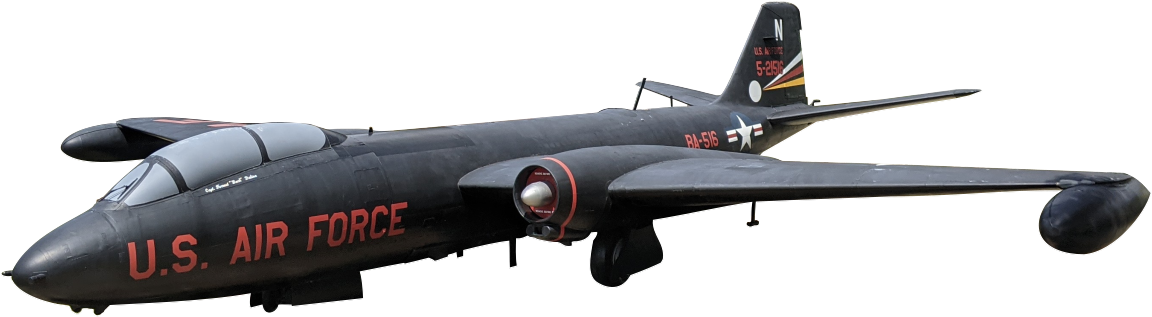
\includegraphics[width=6.5in]{figures/Martin_B-57_Canberra.png}
		\label{fig:title_figure}
	\end{figure} 
	
	\vspace{4cm}
	
	\textbf{Austin R.J. Downey}\\ Department of Mechanical Engineering \\ Department of Civil and Environmental Engineering \\ University of South Carolina, Columbia SC, USA 
	
	\vspace{1cm}
	
	\textbf{Laura Micheli}\\  Department of Civil and Environmental Engineering \\ Catholic University of America, Washington DC, USA
	
	\vspace{2cm}
	
	\today
\end{center}

\pagebreak

\section*{Preface}
This open-source text is designed to offer the reader a complete text on the basics of mechanical vibrations. 

\subsection*{Cover Art}
The B-57 Canberra is an American-built copy of the British English Electric Canberra which first flew in 1949. During initial high-speed flight testing, excessive vibrations were measured on the canopy and a small fairing was added behind the canopy to reduce the aerodynamic load on the canopy and thereby reduce the vibrations. Overall, airframes flight testing is said to have gone very smoothly. 

The B-57 was initially a twin-engined tactical bomber and reconnaissance aircraft but over the years, various versions were produced or modified from the original stock. These include the WB-57F, a specialized strategic reconnaissance version developed for the U.S. Air Force that is still flown by NASA for scientific missions. Of note, in 2011 NASA determined that they needed a third WB-57F to support their mission and an additional WB-57 (s/n 63-13298) was removed from the Air Forces Boneyard in Tucson Arizona after 40 years of storage and returned to operational status. As of 2022, three airframes are still flying for NASA.

The airframe on the cover is the SN 52-1516 and is an EB-57B ``Night Intruder'' which is an electronic countermeasure (ECM) version of the B-57 and is on static display at the Air Force Armament Museum at Eglin Air Force Base, Florida. 

\subsection*{License}
This work is licensed under a Creative Commons Attribution-ShareAlike 4.0 International License[cc-by-sa 4.0]. More information on the Attribution-ShareAlike 4.0 International (CC BY-SA 4.0) can be found at  \url{https://creativecommons.org/licenses/by-sa/4.0/}

\subsection*{Source Code}
The source code for this text is available at \url{https://github.com/austindowney/Open-Vibrations}.




\pagebreak

\tableofcontents

\pagebreak

% Chapter 1 Fundamentals of vibrations
\graphicspath{{Chapter_1_fundamentals_of_vibrations/}} 
\documentclass[12pt,letter]{article}
\usepackage{../downey_format}


\begin{document}
	
	% set the section number, along with figure and equation numbers
	\setcounter{section}{0}	
	\setcounter{figure}{0}   
	\renewcommand\thefigure{\thesection.\arabic{figure}}
	\setcounter{equation}{0}   
	\renewcommand\theequation{\thesection.\arabic{equation}}

	\section{Basic Concepts in Vibrations}

    The study of vibrations, within the broader field of classical mechanics, is the investigation of oscillations that occur about an equilibrium point. Vibrations, both desired and undesired, are present in all mechanical systems and can be helpful (e.g. a soil sieve, rotary sander) or destructive (e.g. an aircraft frame in resonance). The oscillations that form a vibrating system may be periodic (e.g., pendulum) or random (e.g. turbulence in an airplane), or a combination of the two. 

    Vibrations impact our daily lives in a variety of ways, from the sound made by banjo strings that vibrates between 140 and 400 Hz to the 4-6 Hz vibration felt by a passenger in a car seat. The consideration of vibrations, and their associated mathematical modeling, are important factors in the design of mechanical systems. In the material that follows, the fundamental theories of vibration are presented and modeled using fundamental physical principles such as Newton's three laws of motion. These models and analyzed using the mathematical tools of calculus and differential equations. 

	\begin{vibration_case_study}
		Why study vibrations? One day, it could save your life! The British Aircraft Corporation TSR-2 was a strike and reconnaissance aircraft developed during the Cold War by the British Aircraft Corporation (BAC), for the Royal Air Force (RAF). During the second flight test of air-frame XR219, vibration from one of the plane's fuel pump causes a vibration at the resonant frequency of the human eyeball which caused a momentary loss of vision. Test pilot Roland Beamont throttled back one engine to restore his full vision. Roland Beamont was an expert in vibrations, having led the vibration program of the Hawker Typhoon during WW~II. In this role, he fit vibrographs to airplanes to determine the effectiveness of propeller balancing and the testing of seats with vibration isolators. 

		\begin{figure}[H]
			\centering
			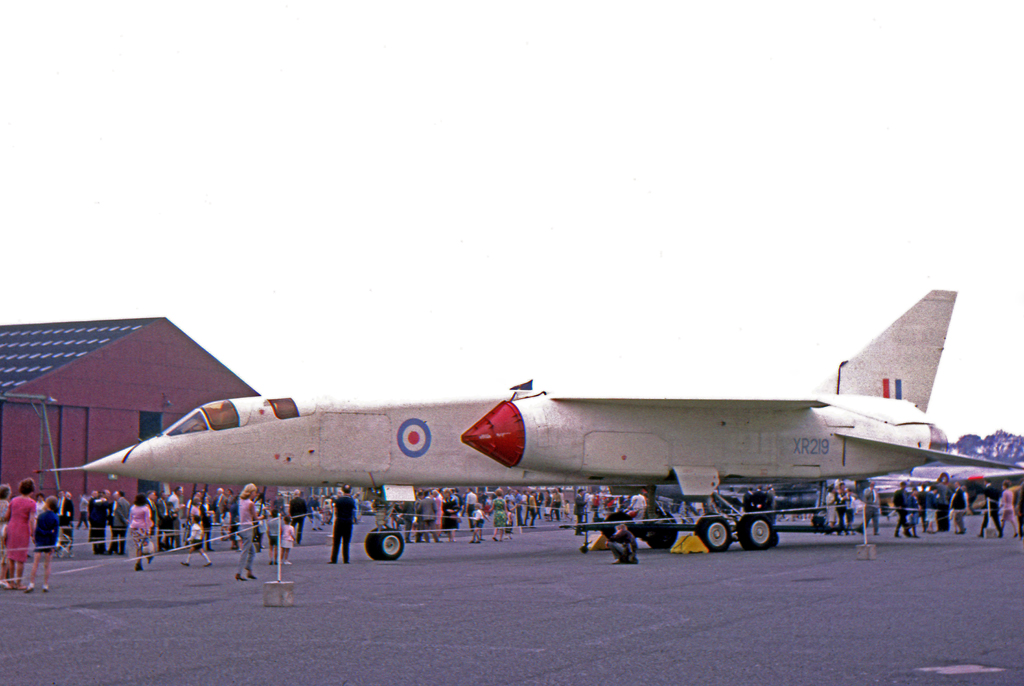
\includegraphics[width=4in]{../figures/TSR_2.jpg}
			\caption{The only BAC TSR-2 prototype to fly, picture taken in 1966 at what is now BAE Warton Lancashire.\protect\footnotemark[1]}
		\end{figure}
		\footnotetext[1]{RuthAS, CC BY 3.0 $<$https://creativecommons.org/licenses/by/3.0$>$, via Wikimedia Commons}	
	\end{vibration_case_study}

	\begin{review}
		Newton's three laws of motion:
		\begin{enumerate}
			\item In an inertial frame of reference, an object either remains at rest or continues to move at a constant velocity unless acted upon by a force.
			\item In an inertial reference frame, the vector sum of the forces $F$ on an object is equal to the mass m of that object multiplied by the acceleration of the object: $F = ma$. (It is assumed here that the mass m is constant)
			\item When one body exerts a force on a second body, the second body simultaneously exerts a force equal in magnitude and opposite in direction on the first body.
		\end{enumerate}
	\end{review}

	\subsection{Single Degree-of-Freedom Systems}
	
        In its simplest form, the phenomenon of vibration is the exchange of energy between potential and kinetic energy. Therefore, a vibrating system must have a component that stores potential energy. This component must also be capable of releasing the energy as kinetic energy. This kinetic energy is stored in the movement of a mass where the measure of this movement is the velocity of the system and the continuous interchange between potential and kinetic energy is the vibration of the system. The simplest vibrating systems can be modeled as a single-degree-of-freedom (1-DOF) system. In a 1-DOF system, one variable can describe the motion of a system. Potential examples of  1-DOF systems include:
		
		\begin{enumerate}
			\item yo-yo
			\item pogo stick
			\item door swinging on axis
			\item throttle (gas pedal)
		\end{enumerate}
				
		\noindent Variables often used for describing 1-DOF systems are $x(t)$,  $y(t)$,  $z(t)$, and  $\theta(t)$.  Examples of 1-DOF systems are presented in figure \ref{fig:Examples_of_1DOF_systems} where the assumption of small displacements is made. Note: we will often drop the ``$(t)$'' for simplicity in this material. 

		\begin{figure}[H]
			\centering
			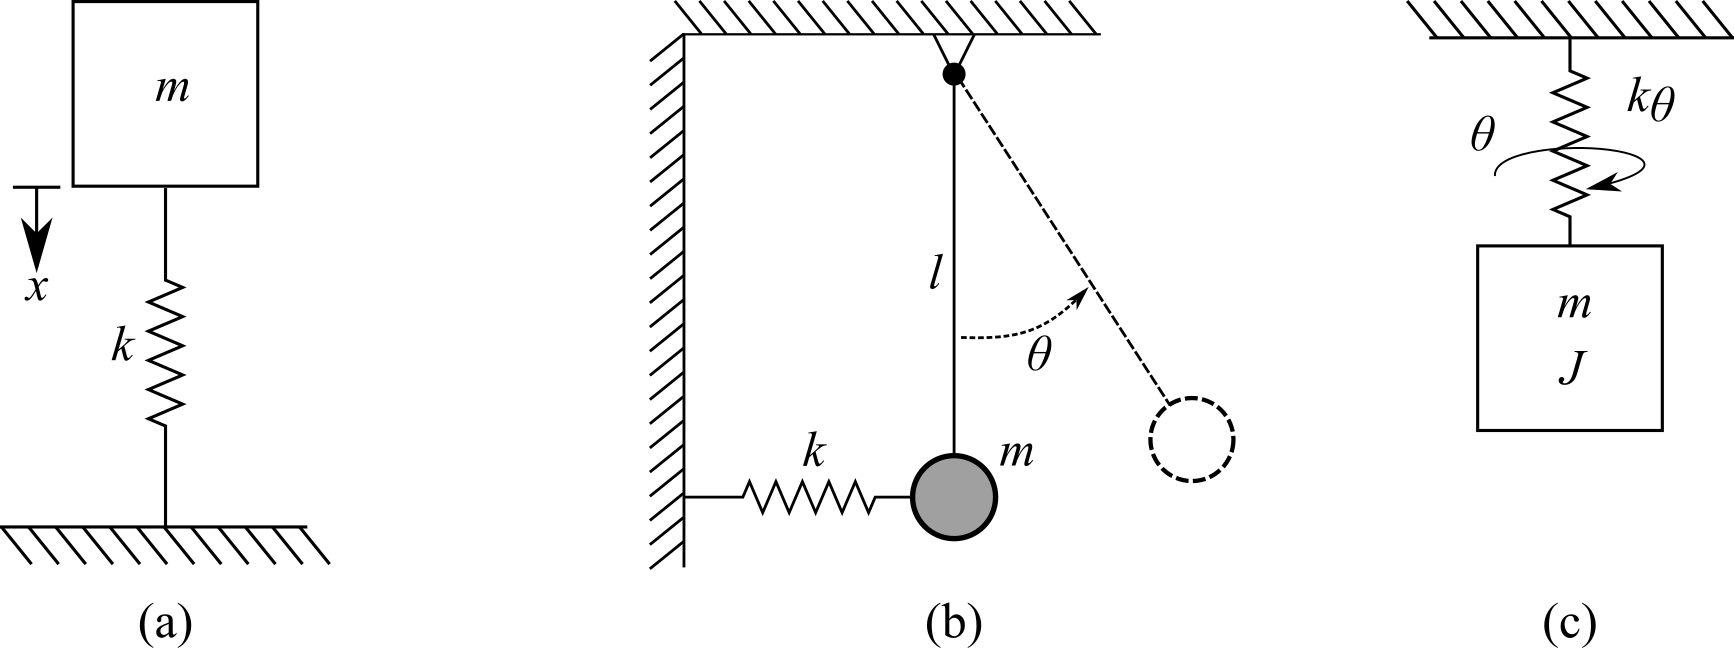
\includegraphics[]{../figures/Examples_of_1DOF_systems.png}
			\caption{Examples of single degree of freedom (DOF) systems showing: (a) a vertical spring-mass system; (b) a simple pendulum; and (c) a rotational spring-mass system.}
			\label{fig:Examples_of_1DOF_systems}
		\end{figure}

		\subsubsection{Spring-Mass Model}

			\quotebox{\large{All models are wrong, but some are useful}}{George E.P. Box (1919 - 2013)}	
							
            Newtonian physics describes the motion of particles in terms of displacement $x$, velocity $\dot{x}$, and acceleration $\ddot{x}$ vectors. Moreover, Newton's second law of motion says that the change in the velocity of mass in motion is a product of the force acting on the mass. A simple way to express this phenomenon is through a spring-mass model as presented in figure  \ref{fig:spring_mass_model_with_point_mass}. These spring-mass models neglect the mass of the spring and concentrate all the mass of the system into a single point. Note that in this case the force vector and mass-acceleration vectors lie on the same axis and as such are collinear. Therefore, these vectors can be easily treated as scalers simplifying the math used in the modeling of the system.     

			\begin{figure}[H]
				\centering
				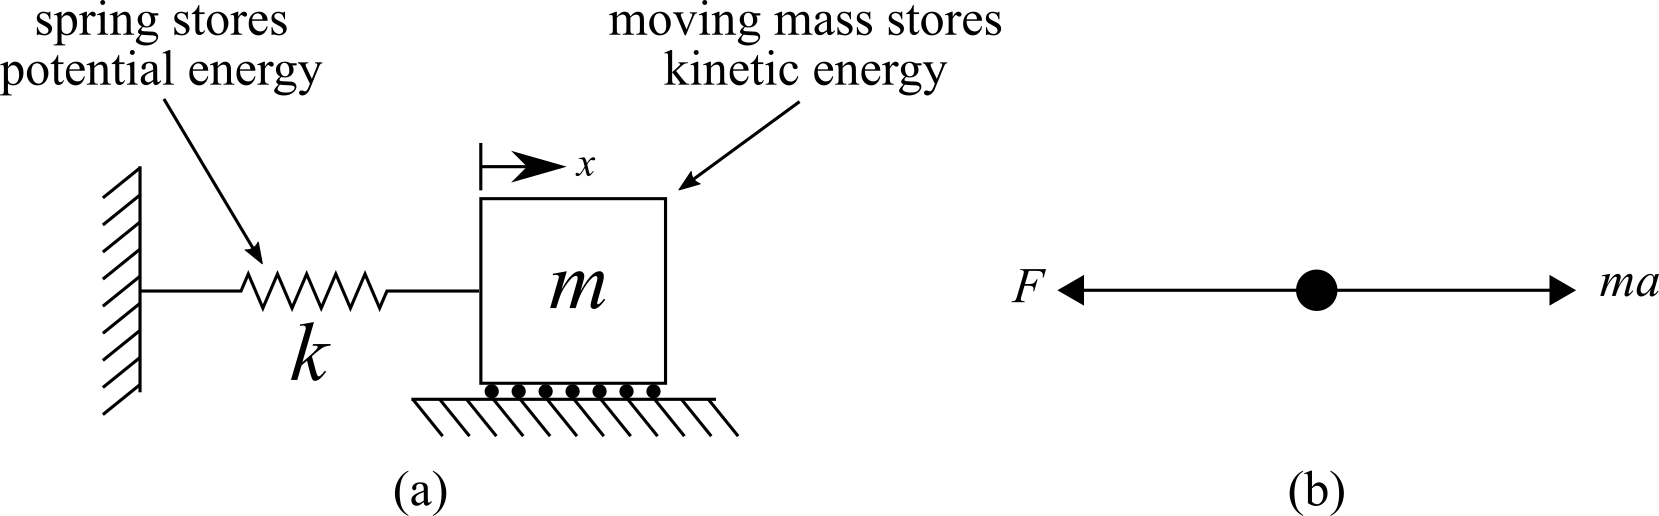
\includegraphics[]{../figures/spring_mass_model_with_point_mass.png}
				\caption{A single-degree-of-freedom (1-DOF) spring-mass model showing: (a) annotated schematic of a mass-spring system; and (b) the equivalent free-body diagram represented as a point-mass system.}
				\label{fig:spring_mass_model_with_point_mass}
			\end{figure}	
		
		\subsubsection{Linear Springs}
	
            Springs are mechanical devices that store energy, moreover, an ideal spring is a theoretical representation of this mechanical device that is massless and responds with a linear increase in force for a unit increase in displacement (i.e. $F=kx$). For simplicity, the springs in the spring-mass models considered in this text are always assumed to be ideal linear springs. A graphical representation of the idealized linear spring is presented in figure \ref{fig:linear_spring_deformation} where a unit force $F$ applied to the free end of the spring results in a unit displacement $x$ of the spring.  The resulting mathematical relationship,  $F=kx$, is known as Hooke's Law. Nonlinear springs add considerable complexity to the modeling of spring-mass systems, therefore, these are not considered in this introductory work. 
			
			\begin{figure}[H]
				\centering
				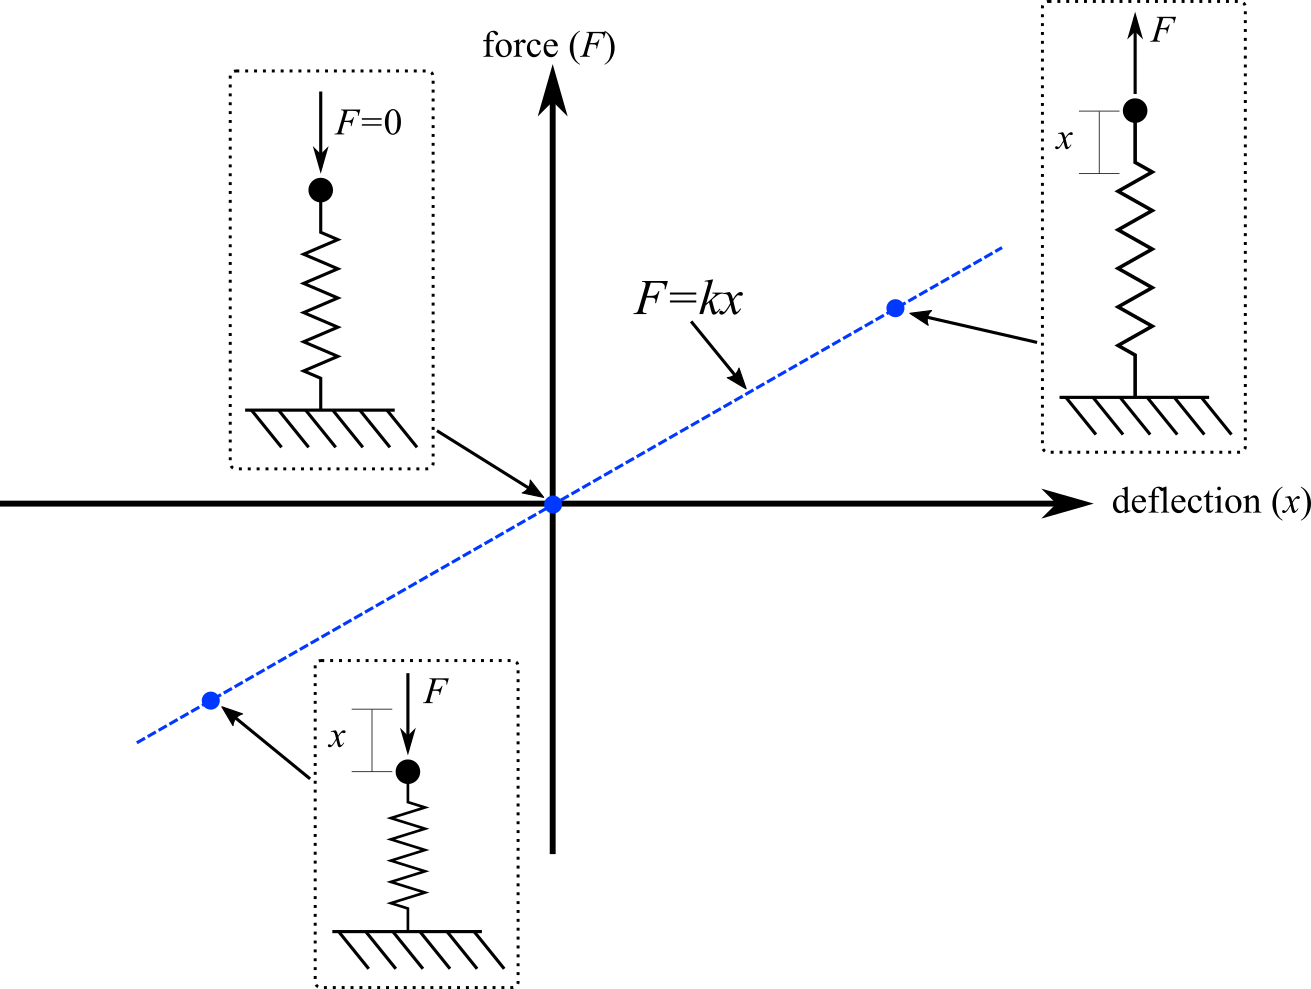
\includegraphics[]{../figures/linear_spring_deformation.png}
				\caption{Force-displacement plot for a linear spring.}
				\label{fig:linear_spring_deformation}
			\end{figure}					


		\begin{vibration_case_study}
			Why study vibrations? Because vibrations form an integral part of how we interact with our world and as such, are an important consideration in product. For example, vibrations in the automotive industry fall within a field of expertise termed Noise Vibration and Harshness (NVH). NVH is important because, within a single company, different levels of NVH will be desired for different market segments and products. 
			
			With a proper understanding of NVH, engineers can design cars that can adapt to their environment or desired use case. Consider the 2019 VW Golf GTI shown in figure~\ref{fig:VW_GTI_Suspension_1}(a) equipped with a dynamic suspension system where the driver can select between `comfort' `normal' and `sport' suspension options. To investigate the effect of these suspension settings, an engineer can install an accelerometer (a sensor used for measuring acceleration) as shown in figure~\ref{fig:VW_GTI_Suspension_1}(b). An important consideration in measuring acceleration is where and how to mount the accelerometer. Here, the accelerometer is mounted in the cup holder to measure the vertical acceleration in the center of the car. 
			\begin{figure}[H]
				\centering
				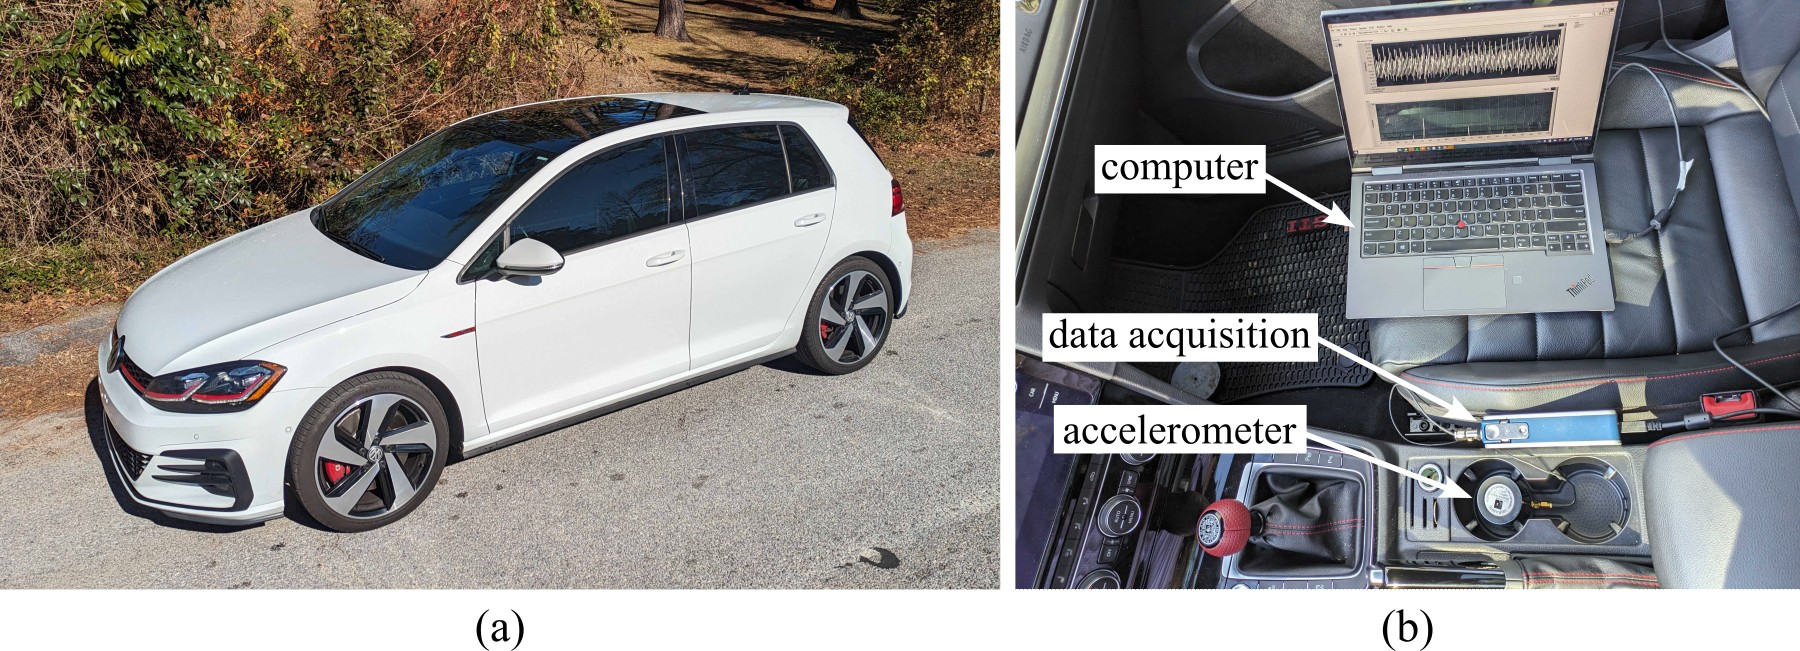
\includegraphics[width=6in]{../figures/VW_GTI_Suspension_1}
				\caption{VW Golf GTI with three suspension modes, showing: (a) the car, and; (b) the accelerometer and data acquisition system used for measuring vibrations.}
				\label{fig:VW_GTI_Suspension_1}
			\end{figure}
			Figure~\ref{fig:VW_GTI_Suspension_2} shows the measured acceleration in the frequency domain for the three suspension modes during 5 minutes of interstate driving. While we will delve into the technical of power spectral density, for now, consider the area under the curve to be representative of the amount of energy in the measured vibrations for each suspension setting. 
			\begin{figure}[H]
				\centering
				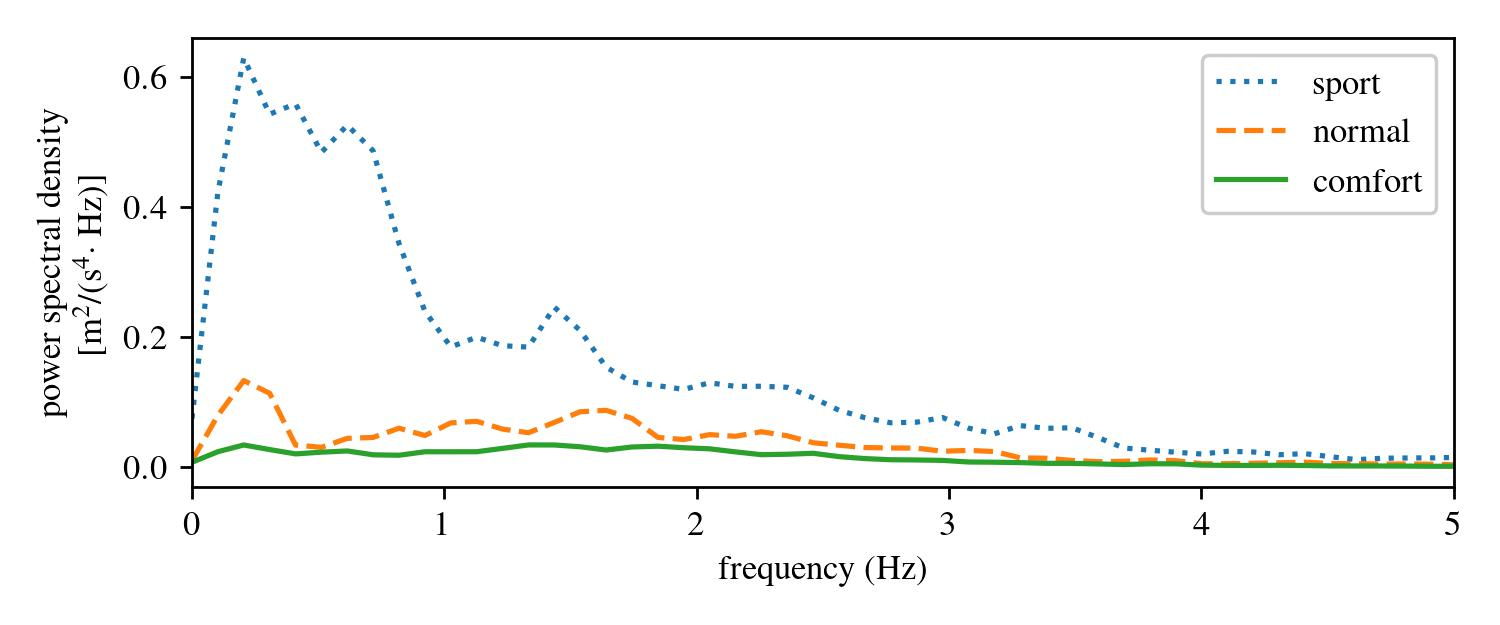
\includegraphics[width=6in]{../figures/VW_GTI_Suspension_2}
				\caption{Response spectrum of the vibrational energy in a VW GTI measured using the experimental setup shown in figure~\ref{fig:VW_GTI_Suspension_1}(b). }
				\label{fig:VW_GTI_Suspension_2}
			\end{figure}
			The sport mode is by far the suspension mode with the firmest ride and the highest amount of measured vibration energy. While a stiff ride is beneficial during spirited driving on a track, the associated NVH level is tiring during prolonged driving. However, the comfort mode adds a considerable amount of damping to the suspension, resulting in a ride quality that is much more amenable to everyday driving. An engineer, using their knowledge of vibrations, could develop systems that enable a single product (such as an automobile or an airplane) to function well in multiple use cases; thereby increasing its usefulness and marketability. 

		\end{vibration_case_study}
		
	\subsection{Equivalent Stiffness}
		
		The generalized concept of stiffness can be directly related to mechanical systems and structural components through Hooke's law. 
		\begin{review}
			Hooke's Law states that the force ($F$) needed to extend or compress a spring by some distance $x$ scales linearly with respect to that distance. This law can be extended to tensional stress of a uniform and elastic bar where the length, area, and Young's modulus of the bar are represented by $l$, $A$, and $E$, respectively. Knowing the tensile stress in the bar:
			\begin{equation}
			\sigma = \frac{F}{A}
			\end{equation} 			
			and the definition of strain:
			\begin{equation}
			\varepsilon = \frac{\Delta l}{l}
			\end{equation} 			
			Hooke's law can be expanded to represent a uniform and elastic bar:
			\begin{equation}
			\sigma = E \varepsilon
			\end{equation} 			
			It follows that the change in length $\Delta l$ can be expressed as:		
			\begin{equation}
			\Delta l = \varepsilon l = \frac{F l}{A E}
			\end{equation} 
			\textbf{Note:} Hooke's law is often expressed using the convention that $F$ is the restoring force exerted by the spring on the applied force at the free end. Defining the stiffness and displacement as $k = \frac{AE}{l}$ and $\Delta l = x$, respectively. The equation for Hooke's Law becomes:
			\begin{equation}
			F = -kx
			\end{equation} 			
			since the direction of the restoring force is opposite the spring displacement.
		\end{review}
	
		\subsubsection{Equivalent Stiffness of Structural Systems}	
		
            For a rod with a uniform cross-section, a direct representation of the system can be developed as expressed in figure \ref{fig:spring_and_bar_mass_vertical} where the vibration along the axis of the rod is to be considered. The stiffness of the rod, $k$, is a measure of the resistance offered by an elastic body to deformation. 

			
			\begin{figure}[H]
				\centering
				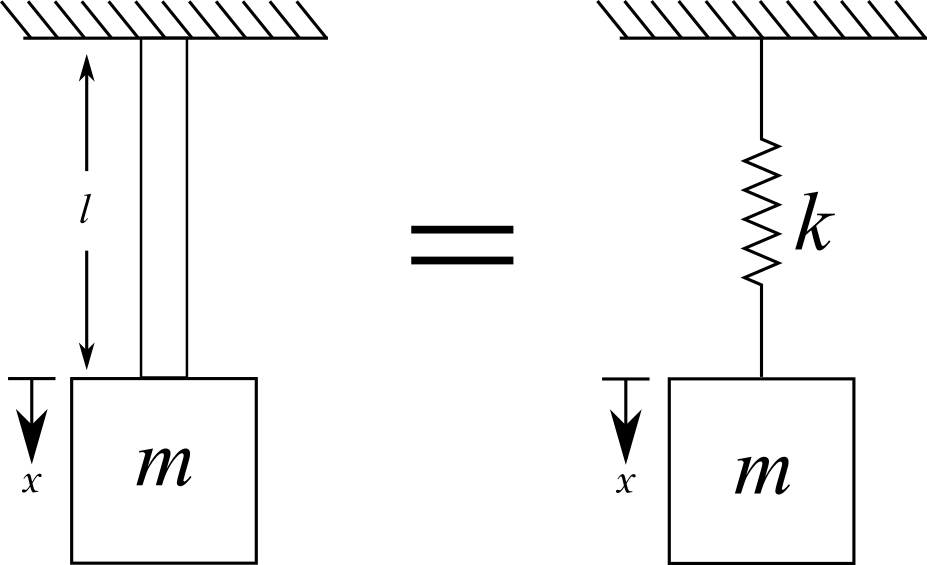
\includegraphics[]{../figures/spring_and_bar_mass_vertical.png}
				\caption{Equivalency between a vertical bar with a mass attached to the bottom and a spring-mass model of the system.}
				\label{fig:spring_and_bar_mass_vertical}
			\end{figure}
			
			For this 1-DOF system, the equation of a spring can be rearranged such that the stiffness can be defined as:
			\begin{equation}
				k=\frac{F}{x}
			\end{equation}
			The stiffness of the spring can be more closely related to material properties of the bar $A$, $E$, and $l$ considering that Hooke's Law for the uniform tension on a bar can be expressed as:
			\begin{equation}
				\sigma = E \varepsilon
			\end{equation}			
			This expression can be expanded into the form:
			\begin{equation}
				\frac{F}{A} = E \Big( \frac{x}{l} \Big)
			\end{equation}					
			rearranging the terms and recalling the expression $k = \frac{F}{x}$ leads to:			
			\begin{equation}
				 k = \frac{EA}{l}
			\end{equation}				
		
			In a similar fashion, we can also solve the equivalent system for a mass at the end of a cantilever beam.
			\begin{figure}[H]
				\centering
				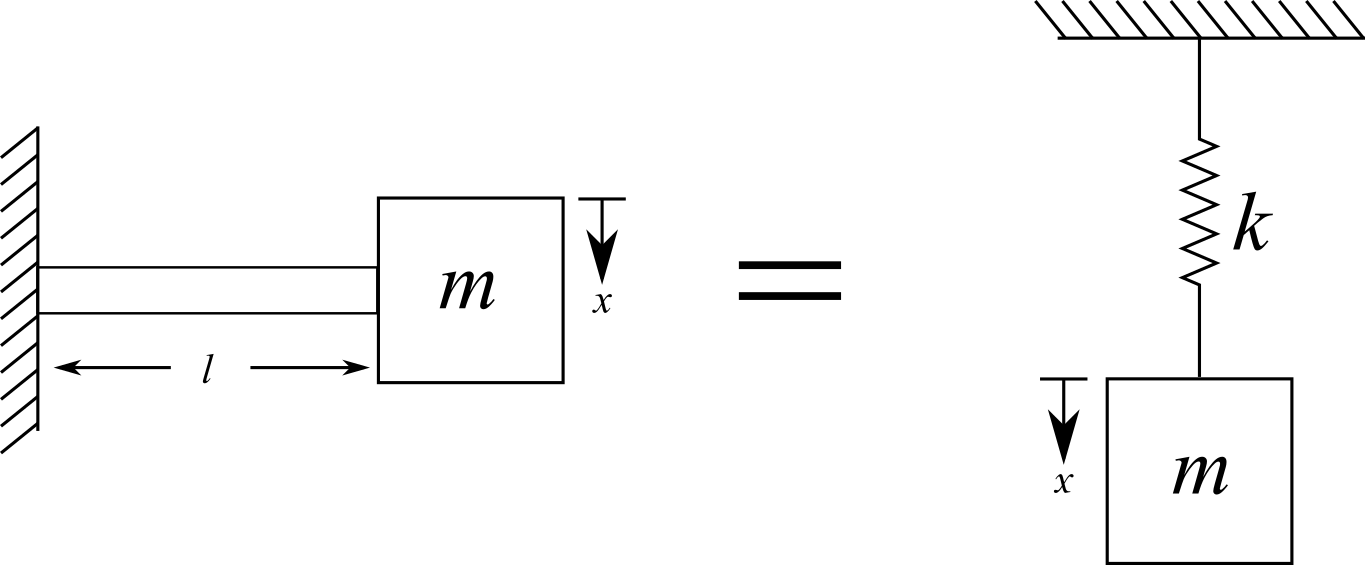
\includegraphics[]{../figures/spring_and_bar_mass_cantilever_beam.png}
				\caption{Equivalency between a cantilever beam and a spring mass system.}
			\end{figure}			
			From engineering mechanics, we can compute the deflection at the point of a beam $\delta$ with a point load $P$. This expression is typically expressed as:
			\begin{equation}
				\delta = \frac{Pl^3}{3EI}
			\end{equation}					
			If we transform this equation into our variable system by exchanging $P$ for $F$ and $\delta$ for $x$. Thereafter, the point load is replaced with the equivalent force $F$ generated by the mass and the pull of gravity($mg$). As before, knowing that the stiffness of the system can be expressed as $k=F/x$ we can show that:
			\begin{equation}
				k = \frac{3EI}{l^3}
			\end{equation}	


			\begin{example}
    			
    			Considering the rod diagrammed below; calculate an equivalent spring constant for the rod using the length of the rod $l$, its area $A$, and Young's modulus $E$ for a compressive force $F$ that compresses the rod a distance $x$. Additionally, is a linear spring a useful model for a rod under compression? What if the rod is under tension?
        
		 		\begin{figure}[H]
		 			\centering
		 			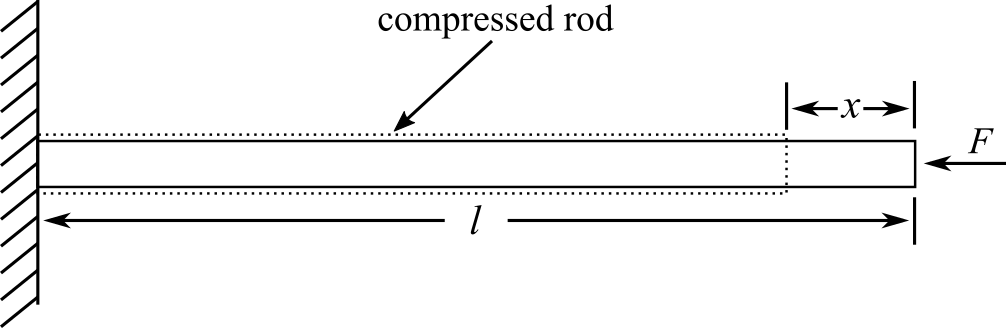
\includegraphics[]{../figures/compressed_cantilever_rod.png}
		 			\caption{Compressed cantilever rod. }
		 		\end{figure}	   
       
			    \noindent \textbf{Solution:}

				 The rod shortens by a distance $x$ under the axial force $F$, this can be related to the equation of a linear spring $F=kx$ by recalling from solid mechanics that the elongation (or shortening) of a rod is expressed as 
			
			    \begin{eqnarray}
			    x=\frac{x}{l}l=\varepsilon l = \frac{\sigma}{E}l = \frac{Fl}{AE}
			    \end{eqnarray}    
			    
			    where  $\varepsilon = \frac{x}{l}$ is the strain value and $\sigma = F/A$ is the stress induced in the rod. Combining this expression with the equation of a linear spring yields:
			    
			    \begin{eqnarray}
			    k = \frac{F}{x}= \frac{AE}{l}
			    \end{eqnarray}     
			   
			    As per the usefulness of the linear spring to represent an axial rod under compression or tension, this would be application-specific but could generally be considered an excellent first-order approximation.  
			
			\end{example}

		\subsubsection{Springs in Series and Parallel}
			
			In many cases, it becomes necessary to model a mechanical system as a set of springs (e.g., a composite material, a table with multiple legs).  For these systems, or for systems with more than one spring acting on a body, equivalent stiffness can be calculated as:
			\begin{figure}[H]
				\centering
				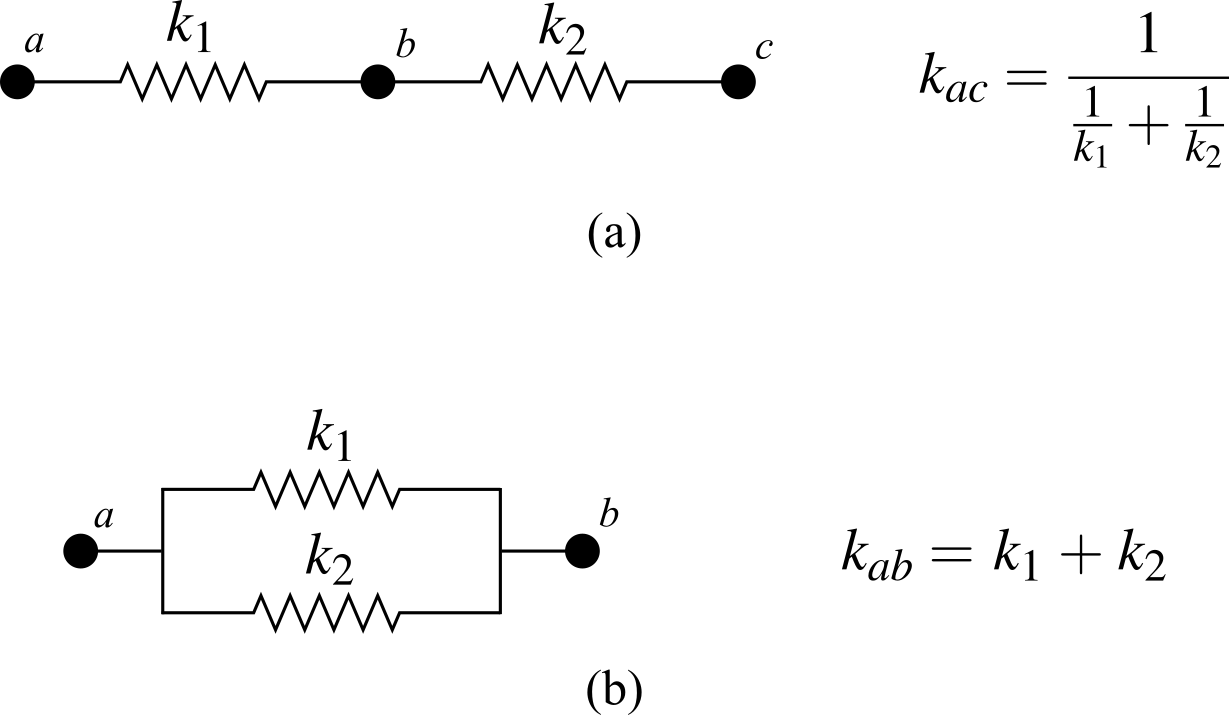
\includegraphics[]{../figures/equivalent_stiffness.png}
				\caption{Equations for calculating the equivalent stiffness of two springs ($k_1$ and $k_2$); (a) in series; and (b) in parallel.}
			\end{figure}	
			These are derived considering the displacement $\delta$ of the systems. For two springs in series:
			\begin{figure}[H]
				\centering
				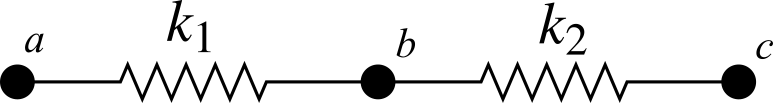
\includegraphics[]{../figures/equivalent_stiffness_series.png}
				\caption{Two springs $k_1$ and $k_2$ combined in series.}
			\end{figure}			
			\noindent where the total displacement is 
			\begin{equation}
				\delta_{ac} = \delta_{ab} + \delta_{bc}
			\end{equation}
			Using the equation for stiffness $k=F/\delta$, this converts to:
			\begin{equation}
				\frac{F}{k_{ac}} = \frac{F}{k_{1}} + \frac{F}{k_{2}}
			\end{equation}
			As $F$ is the same throughout the system, we can cancel out $F$. Solving for the equivalent stiffness yields:
			\begin{equation}
				k_{ac} = \frac{1}{\frac{1}{k_1}+\frac{1}{k_2}}
			\end{equation}
			Similarly for a system of springs in parallel:
			\begin{figure}[H]
				\centering
				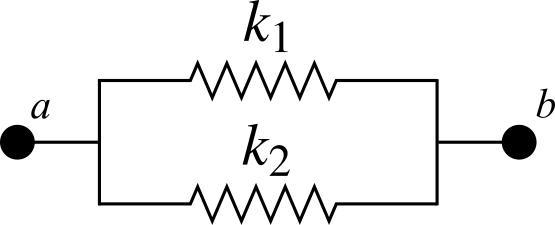
\includegraphics[]{../figures/equivalent_stiffness_parallel.png}
				\caption{Two springs $k_1$ and $k_2$ combined in parallel.}				
			\end{figure}			
			\noindent The displacement in both springs is the same, so the total displacement is 
			\begin{equation}
				\delta_{ab} = \delta_{\text{1}} =  \delta_{\text{2}} = \delta
			\end{equation}
			The forces in the direction of spring elongation sum to zero, therefore:
			\begin{equation}
				F_{ab} = F_{\text{1}} +  F_{\text{2}}
			\end{equation}			
			Substituting the displacement and stiffness into the force equation yields:
			\begin{equation}
				\delta k_{ab} = 	\delta k_{1} +  \delta k_{2}
			\end{equation}				
			this simplifies to:
			\begin{equation}
				k_{ab} = k_1+k_2
			\end{equation}
			


			\begin{example}

				Calculate the equivalent stiffness of the following system:
				\begin{figure}[H]
					\centering
					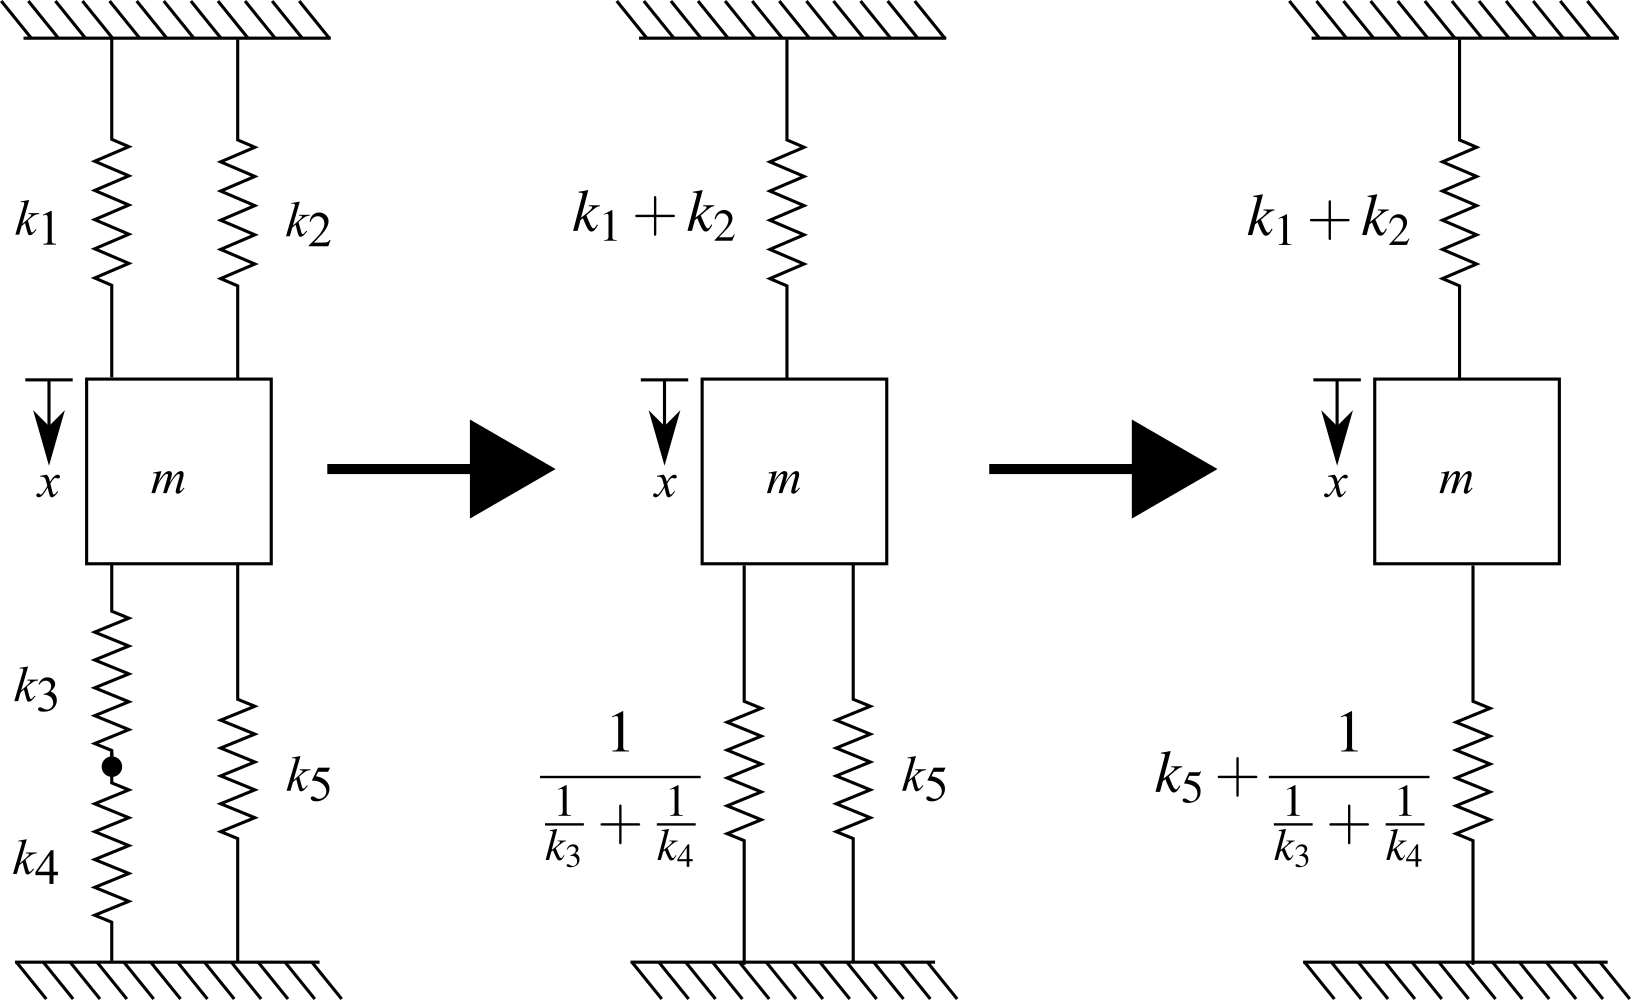
\includegraphics[]{../figures/equivalent_mass_and_spring_system_1.png}
					\caption{Equivalent stiffness for springs in series and parallel.}
				\end{figure}	
				The springs are combined as shown, using the equations defined before.  Now, considering that the displacement ($\delta$) of the top spring, and the bottom spring are the same we can state the total stiffness $k$, which is the summation of the two. Therefore,    
				\begin{figure}[H]
					\centering
					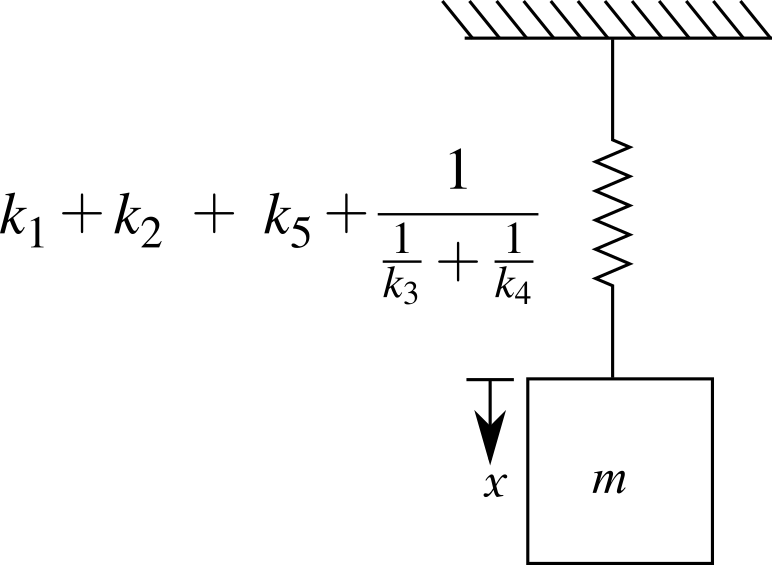
\includegraphics[]{../figures/equivalent_mass_and_spring_system_2.png}
					\caption{A spring mass system simplified down form springs in series and parallel..}
				\end{figure}	
%				until a final $k$ value can be obtained:
%				\begin{equation}
%					k=k_1+k_2+k_5+\frac{1}{\frac{1}{k_3}+\frac{1}{k_4}}
%				\end{equation}		
				\noindent where the final addition, $(k_1+k_2) + (k_5+\frac{1}{\frac{1}{k_3}+\frac{1}{k_4}})$ is applied at two springs in parallel as each spring is connected between the mass and the fixity. Rearranging this new expression to get a common denominator:
				\begin{equation}
					k= \frac{(k_1+k_2+k_5)(k_3+k_4)+k_3k_4}{k_3+k_4}  
				\end{equation}				
%				For an arbitrary mass, $m$, the undamped frequency $\omega_n$ can be calculated as:
%				\begin{equation}
%					\omega_n = \sqrt{\frac{k}{m}} = \sqrt{\frac{(k_1+k_2+k_5)(k_3+k_4)+k_3k_4}{m(k_3+k_4)} }
%				\end{equation}				
			\end{example}	

					
	\subsection{Equation of Motion for an Oscillating System}			
			
        An Equation of Motion (EOM) is an equation that provides a basis for modeling a vibrating system about its equilibrium point and relates the transfer of the potential energy from the spring to the kinetic energy mass. In developing the EOM we assume that any surfaces are frictionless and as such, no energy is extracted from the vibrating system. Referencing the 1-DOF system in figure \ref{fig:EOM_1-DOF-mass_horizontal}(a), and assuming the mass only moves in the $x$ direction, the only force acting on the mass in the $x$ direction is the force that results from the elongation of the spring as annotated in figure \ref{fig:EOM_1-DOF-mass_horizontal}(b). Therefore, the sum of forces along the $x$ axis must equal the mass ($m$) times the acceleration of the mass ($a\dot{x}$). 

		\begin{figure}[H]
			\centering
			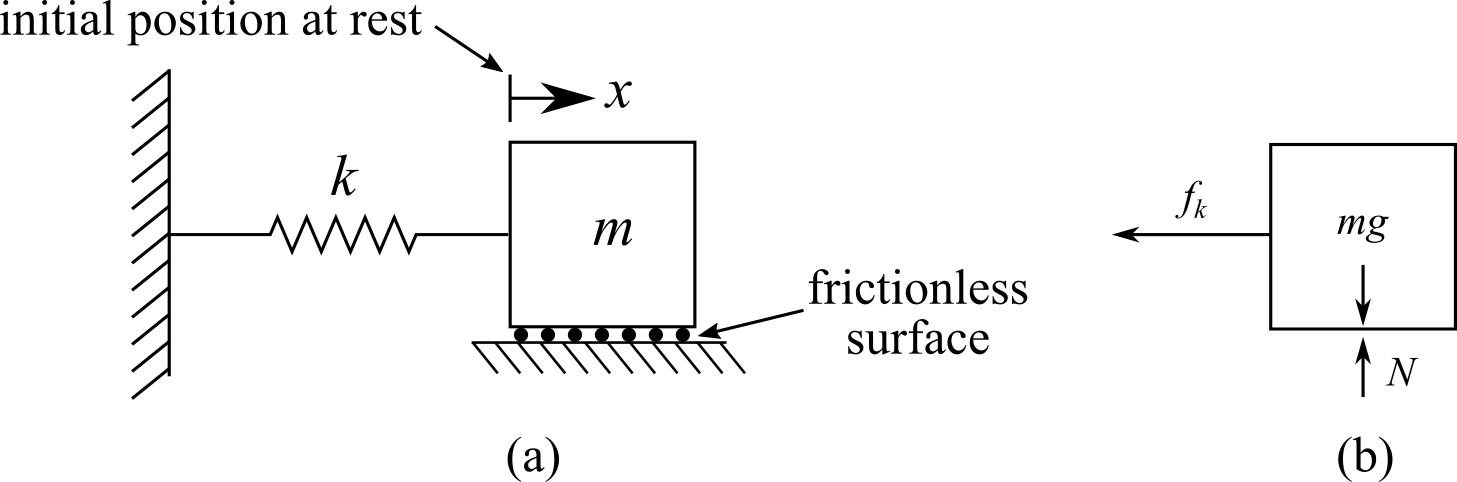
\includegraphics[]{../figures/EOM_1-DOF-mass_horizontal.png}
			\caption{A spring-mass model of a 1-DOF system showing: (a) a schematic of the system; (b) a free-body diagram of the system at its initial position.}
			\label{fig:EOM_1-DOF-mass_horizontal}
		\end{figure}			
		
		Considering that positive displacements are to the right, the standard form of the equation of motion for an undamped system without any excitation is expressed as:  
		\begin{equation}
			s_1 \ddot{x} + s_2 x = 0
		\end{equation}			
		where $s_1$ and $s_2$ are constants to be determined for the specific system. A systematic approach to obtaining the free-body diagram (FBD) of a system under vibration can be expressed in three steps:
		\begin{enumerate}
			\item Draw a free-body diagram (FBD) at the system's equilibrium and displaced position (without a displacing force).
			\item Apply Newton's second law to both FBDs ( equilibrium and displaced).
			\item Combine the equations to write the EOM in standard form with the forcing component on the right-hand side. For free vibration, the forcing component is 0. 
		\end{enumerate}
			
		Solving these three steps for 1-DOF system presented in figure \ref{fig:EOM_1-DOF-mass_horizontal} results in the EOM:
		\begin{equation}
			m \ddot{x} + k x = 0
		\end{equation}

		\begin{review}
			A second-order linear homogeneous differential equation has the form:
			
			\begin{equation}
			 a \ddot{x} + b \dot{x} + cx = 0
			\end{equation}
		
			\noindent The EOM for a 1-DOF system under a free vibration is a second-order differential equation due to acceleration ($\ddot{x}$) being the second derivative of displacement ($x$) and homogeneous as the forcing function (right-hand side of the equations) is zero. In EOM's current form, $a=m$, $b=0$,  and $c=k$. In future work, $b$ will account for damping in the vibrating system.     
		\end{review}

					
		\begin{example}			
			
			Considering the system:
			\begin{figure}[H]
				\centering
				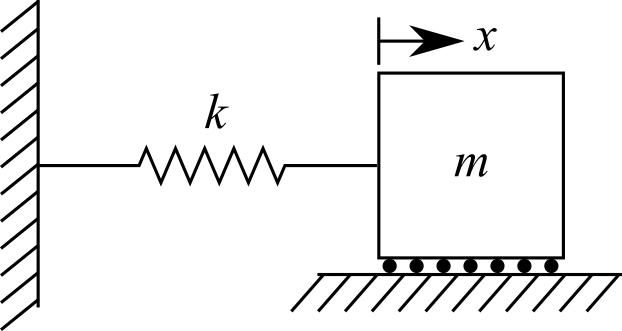
\includegraphics[]{../figures/1-DOF-spring_mass_horizontal.png}
				\caption{A 1 DOF spring mass system with movement in the horizontal direction}
			\end{figure}		
			
			\textbf{Step-1}
			Define the direction of displacement, and draw the FBD for the equilibrium and displaced state.  
			\begin{figure}[H]
				\centering
				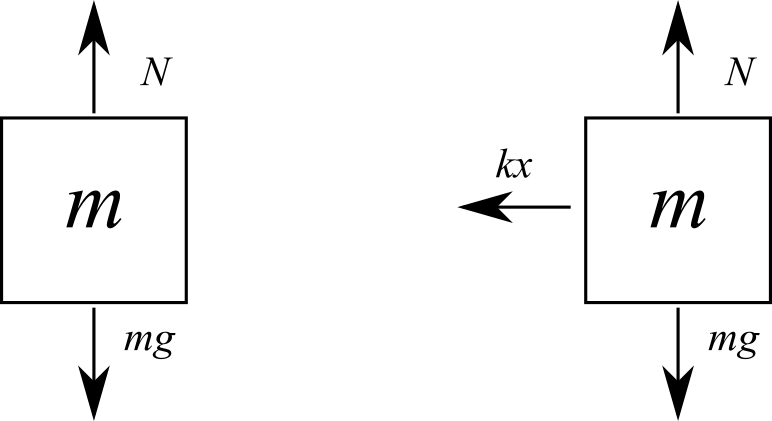
\includegraphics[width=0.45\textwidth]{../figures/1-DOF-mass_horizontal_FBD.png}\\
				equilibrium state \hspace{3cm} displaced state
				\caption{Equivalent forces for a 1 DOF spring mass system with movement in the horizontal direction}
			\end{figure}		
			\noindent The equation for the equilibrium state is:
			\begin{equation}
			\rightplus \sum F_x = 0
			\end{equation}
			and in the displaced state:
			\begin{equation}
			\rightplus \sum F_x = -kx
			\end{equation}		
			This equation does not equal zero as the FBD does not account for the restoring force. 
	
			\noindent	\textbf{Step-2} Apply Newton's second law (we want to store energy in the kinetic state) of motion to the sum of forces for the displaced position we get: 		 		
			\begin{equation}
			ma = m\ddot{x} = \rightplus \sum F_x = -kx
			\end{equation}			
			\begin{equation}
			m\ddot{x} = -kx
			\end{equation}				
			\textbf{Step-3} Rearrange in the Equation to construct an EOM: 			
			\begin{equation}
			m\ddot{x} + kx = 0
			\end{equation}		
		\end{example}			

		\begin{example}	
			Some systems will have an initial displacement, as the system will oscillate around this position we need to define the EOM about this position. Considering the system:
			\begin{figure}[H]
				\centering
				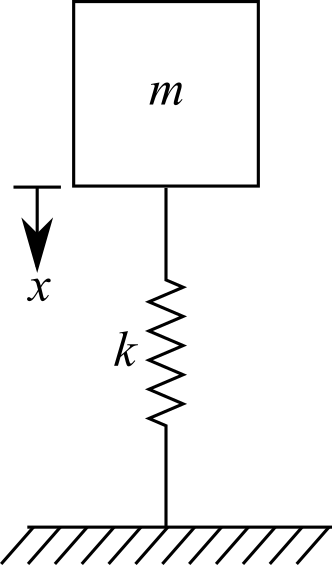
\includegraphics[]{../figures/1-DOF-spring_mass_vertical.png}
				\caption{A 1 DOF spring mass system with movement in the vertical direction}
			\end{figure}		
			\noindent \textbf{Step-1}
			Define the direction of displacement, and draw the FBD for the equilibrium and displaced state.  
			\begin{figure}[H]
				\centering
				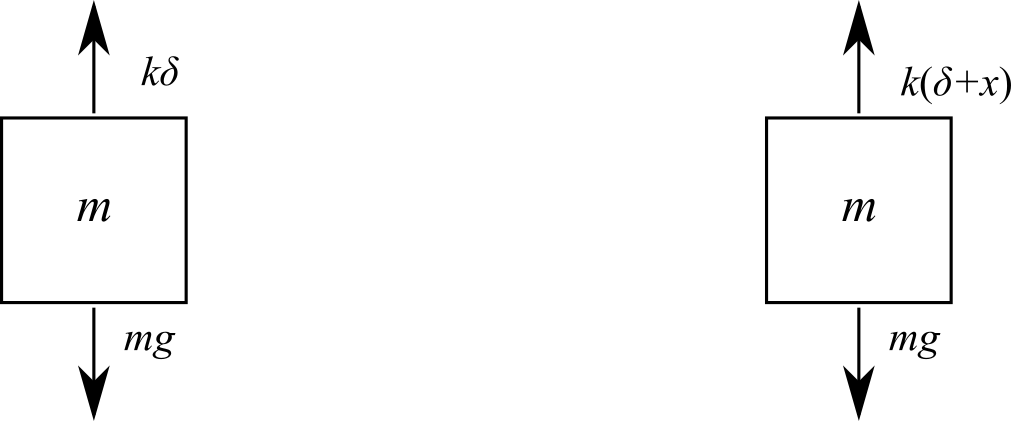
\includegraphics[]{../figures/1-DOF-spring_mass_vertical_FBD.png}\\
				equilibrium state \hspace{3cm} displaced state
				\caption{Equivalent forces for a 1 DOF spring mass system with movement in the vertical direction}
			\end{figure}		
			\noindent The equation for the equilibrium state is:
			\begin{equation}
				\downplus \sum F_x = mg - k\delta = 0
			\end{equation}
			and in the displaced state:
			\begin{equation}
				\downplus \sum F_x =mg -k(\delta + x)
			\end{equation}	
			This equation does not equal zero as the FBD does not account for the restoring force.	
			
			\noindent \textbf{Step-2} Apply Newton's second law (we want to store energy in the kinetic state) of motion to the sum of forces for the displaced position we get: 		
			\begin{equation}
				m\ddot{x} = \downplus \sum F_x =mg -k\delta -kx
			\end{equation}
			We can than use the information from the equilibrium state to cancel out some terms, this becomes:
			\begin{equation}
				m\ddot{x} = -kx
			\end{equation}				
			\textbf{Step-3} Rearrange in the Equation to construct an EOM: 					
			\begin{equation}
				m\ddot{x} + kx = 0
			\end{equation}			
		\end{example}		


		\begin{vibration_case_study}
			Why study vibrations? One day, it could save your job! For a project to be successful they need to be completed on time and within budget. Consider the Ling-Temco-Vought (LTV) XC-142  which was a tilt-wing experimental aircraft developed in the '60s for the US military and later turned over to NASA. During testing, the cross-linked driveshaft produced excessive vibration and noise which resulted in a high pilot workload. In general, the aircraft's cross-linked driveshaft was the main technical issue that caused the military to lose interest in the project. 
			
			\begin{figure}[H]
				\centering
				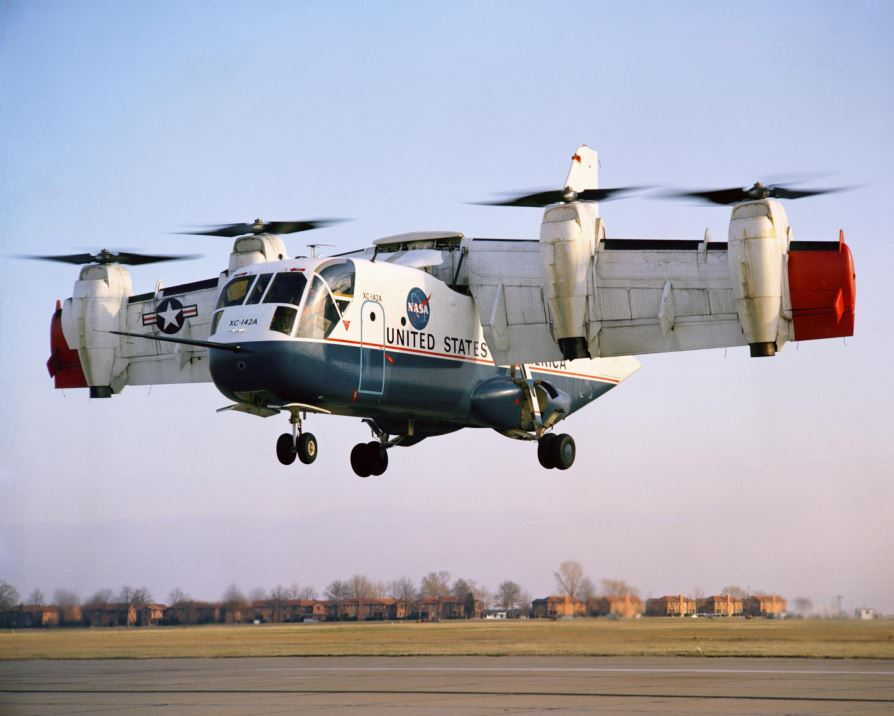
\includegraphics[width=4in]{../figures/Ling_Temco_Vought_XC_142A.jpg}
				\caption{A Ling-Temco-Vought XC-142A tested at the NASA Langley Research Center in 1969. \protect\footnotemark[1]}
			\end{figure}
			\footnotetext[1]{NASA,  Photograph published in Winds of Change, 75th Anniversary NASA publication, by James Schultz, Public domain, via Wikimedia Commons}	
		\end{vibration_case_study}




	
\end{document}



% Chapter 2 Free Vibrations
\documentclass[12pt,letter]{article}
\usepackage{../downey_format}


\begin{document}
	
	% set the section number, along with figure and equation numbers
	\setcounter{section}{1}	
	\setcounter{figure}{0}   
	\renewcommand\thefigure{\thesection.\arabic{figure}}
	\setcounter{equation}{0}   
	\renewcommand\theequation{\thesection.\arabic{equation}}
	\section{Free Vibration of Single-Degree-of-Freedom Systems}





			
		Vibrations (i.e. the exchange of potential and kinetic energy) require oscillatory motion that may repeat itself regularly or irregularly. A motion that is repeated at time intervals is called periodic motion. If this motion has a single frequency and amplitude it is called simple harmonic motion are represents the most basic form of oscillatory motion as depicted in figure \ref{fig:oscillatorymotion}.  For a 1-DOF system, simple harmonic motion is defined as a periodic motion where the restoring force is directly proportional to the displacement and acts in the direction opposite to that of displacement.	
		

		\begin{figure}[H]
			\centering
			\includegraphics[]{../figures/oscillatory_motion.png}
			\caption{Oscillatory motion for a single degree of freedom system showing (a) periodic motion; and (b) simple harmonic motion.}
			\label{fig:oscillatorymotion}
		\end{figure}

		Given the nature of simple harmonic motion, constant amplitude, and frequency, the wave starting at the origin $O$ can be modeled at a point on the end of a vector with length $A$ rotating at a constant angular velocity $\omega_\text{n}$ where the angle from the origin of the vector is $\phi$, defined as $\phi = \omega t$. Where $\omega$ is the lowercase Greek letter Omega and $\phi$ is the lowercase Coptic letter phi. This is similar to a Greek phi ($\varphi$) and either can be used in this context. The subscript $n$ on $\omega$ denotes that this frequency relates to the natural frequency of the system, the only frequency in simple harmonic motion. A visualization of the harmonic motion obtained from projecting the point on the edge of a vector onto the $\omega_\text{n} t$ space is presented in figure \ref{fig:Harmonic_Motion}. 

		\begin{figure}[H]
			\centering
			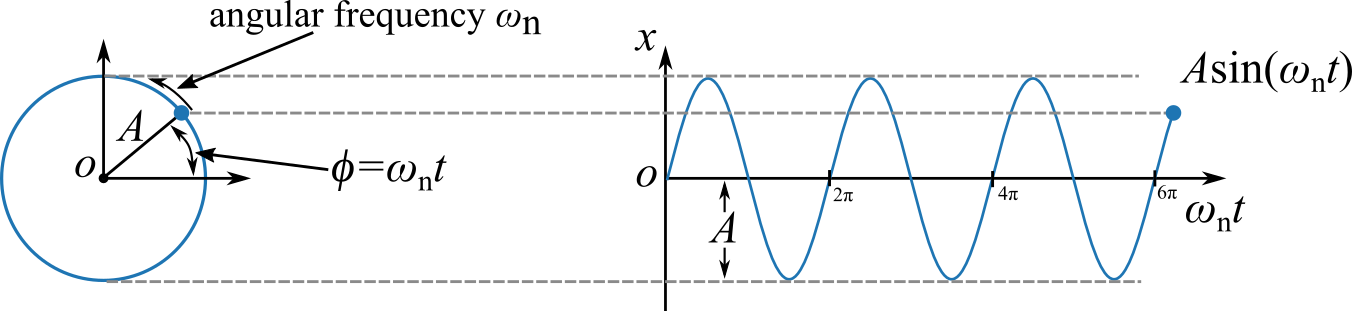
\includegraphics[]{../figures/harmonic_motion.png}
			\caption{Harmonic motion represented at the projection of a point on the end of a vector moving on a circle. Note the axis $\omega_\text{n} t$.}
			\label{fig:Harmonic_Motion}
		\end{figure}

	\subsection{Mathematical Modeling of Free Vibration}

		The Development of a mathematical model for a system under free vibration would enable the practitioner to predict, or model, the vibrating system of interest.  Therefore, considering the following system, 
		
		\begin{figure}[H]
			\centering
			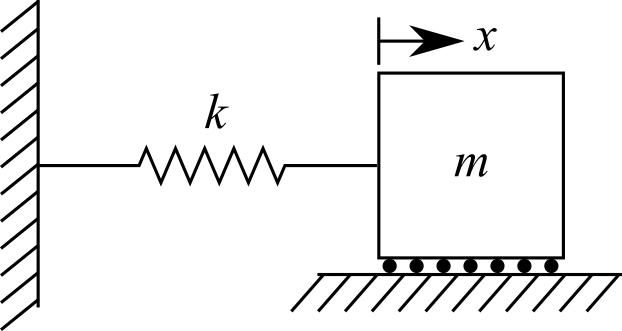
\includegraphics[]{../figures/1-DOF-spring_mass_horizontal.png}
			\caption{1-DOF spring-mass system.}
		\end{figure}
		\noindent can be modeled expressed with the following EOM
		\begin{equation}
			m\ddot{x}(t) + kx(t) = 0
			\label{eq:EOM}
		\end{equation}		
		it becomes prudent to solve this homogeneous ordinary differential equation (ODE) to obtain a model of the vibrating system. The simplest method for solving an ODE is to propose a solution based on observations of a vibrating physical system. Figure \ref{fig:Harmonic_Motion_2.png} reports and annotates the key components from an observation of a vibrating system. 
		
		\begin{figure}[H]
			\centering
			\includegraphics[]{../figures/harmonic_motion_2.png}
			\caption{Summary of the temporal response for a 1-DOF system.}
			\label{fig:Harmonic_Motion_2.png}
		\end{figure}
		\noindent where $x_0$ and $v_0$ are the is the displacement and velocity at $t$=0 (i.e. the initial displacement). 
				

		A mathematical expression can now be formulated to represent the observed simple harmonic motion. This expression can be based on the projection of a point on a vector (transposed into the time domain) or assembled from constituent parts as done in what follows. Solving for a location $x$, at a time $t$; $x(t)$, the various characteristics of the expression can be identified:

		\subsubsection{Solve for the Natural Frequency ($\omega_\text{n}$) of the System }
				
			\begin{itemize}
				\item System oscillates $\rightarrow$ a sin function models this 
				\item System oscillates at different speed $\rightarrow$ use a parameter to adjust $\omega_\text{n}$ in rad/s. 
				\item Systems have different amplitudes $\rightarrow$ use a parameter to adjust $A$ in meters.
				\item System has different starting points $\rightarrow$ use a parameter to adjust $\phi$ in rad. 
			\end{itemize}

			\noindent Using these four constituent components, an equation can be proposed: 
			\begin{equation}
				{x}(t) = A\text{sin}(\omega_\text{n} t + \phi)
			\end{equation}
			Take the derivative to get velocity:
			\begin{equation}
				\dot{x}(t) = A\omega_\text{n}\text{cos}(\omega_\text{n} t + \phi)
			\end{equation}
			Take the derivative again to get acceleration:
			\begin{equation}
			\ddot{x}(t) = -A\omega_\text{n}^2\text{sin}(\omega_\text{n} t + \phi)
			\end{equation}
			Substituting $x$ and $\ddot{x}$ into the EOM for the considered 1-DOF system ($m\ddot{x}(t) + kx(t) = 0$) yields:
			\begin{equation}
				m\big(-A\omega_\text{n}^2\text{sin}(\omega_\text{n} t + \phi)\big) + k\big(A\text{sin}(\omega_\text{n} t + \phi)\big) = 0
			\end{equation}
			Thereafter, dividing both sides by $A\text{sin}(\omega_\text{n} t + \phi)$ results in the expression:
			\begin{equation}
				-m\omega_\text{n}^2+k = 0
			\end{equation}
			This expression can be rearranged into the more useful standard form:
			\begin{equation}
				\omega_\text{n}= \sqrt{\frac{k}{m}}
				\label{eq:natural_frequency}
			\end{equation}
			Equation \ref{eq:natural_frequency} represents a solution to the EOM  presented in equation \ref{eq:EOM}. This solution is not in the form of an ODE  so, therefore, we can experientially prove that this is the correct solution. For example, we could build a system with known mass and stiffness and measure the natural frequency of the system. Equation \ref{eq:natural_frequency} equation leads to:
			\begin{equation}
				T= \frac{2 \pi}{\omega_\text{n}}
			\end{equation}
			where $T$ is the period of oscillations and 
			\begin{equation}
				f_n= \frac{\omega_\text{n}}{2 \pi}
			\end{equation}
			where $f_n$ is the frequency of the oscillations. 
					
		\subsubsection{Solve for Initial Phase ($\phi$) of the System }
			The EOM is a second-order ODE so there needs to exist two initial conditions (constants) to solve it. For the systems under consideration, the displacement ($x$) and velocity ($\dot{x}$ or $v$) at $t=0$ are the initial conditions. For simplicity, these are written as 
			\begin{equation}
				x(0) = x_0  
			\end{equation}			
			\begin{equation}
				\dot{x}(0) = v(0) = v_0 
			\end{equation}			
			Setting the equation to its initial state $t=0$, the equations for displacement and velocity can be simplified to: 
			\begin{equation}
				{x}(0) = x_0 = A\text{sin}(\omega_\text{n} 0 + \phi) = A\text{sin}(\phi)
				\label{eq:x_0=Asintheta} 
			\end{equation}
			\begin{equation}
				\dot{x}(0) = v_0 = A\omega_\text{n}\text{cos}(\omega_\text{n}0 + \phi) = A\omega_\text{n}\text{cos}(\phi)
				\label{eq:v_0=Aomegacosphi} 
			\end{equation}
			Thereafter, mathematical meanings for $\phi$ and $A$ can be derived. To do this, $\phi$  can be solved for by rearranging equations \ref{eq:x_0=Asintheta} and \ref{eq:v_0=Aomegacosphi} for $A$:
			\begin{equation}
				A = \frac{x_0}{\text{sin}(\phi) }
			\end{equation}
			and:
			\begin{equation}
				A = \frac{v_0}{\omega_\text{n}\text{cos}(\phi)}
			\end{equation}
			Setting these two equations equal to each other cancels out A and creates:
			\begin{equation}
				\frac{x_0 \omega_\text{n}}{\text{sin}(\phi)} = \frac{v_0}{\text{cos}(\phi)} 
			\end{equation}
			therefore:
			\begin{equation}
				\frac{x_0\omega_\text{n}}{v_0} = \frac{\text{sin}(\phi)}{\text{cos}(\phi)}
			\end{equation}
			finally:
			\begin{equation}
				\phi = \text{tan}^{-1}\bigg(\frac{x_0\omega_\text{n}}{v_0}\bigg)
			\end{equation}
			
		\subsubsection{Solve for Amplitude ($A$) of the System }
			
			The amplitude of the vibrating system ($A$) is solved for in a similar manner to $\phi$ where the expressions for $x$ and $\dot{x}$ are solved for at $t=0$ and rearranged as to isolate $\phi$. This operation results in the equations:  
			\begin{equation}
				\text{sin}(\phi) = \frac{x_0}{A}
			\end{equation}
			and:
			\begin{equation}
				\text{cos}(\phi) = \frac{v_0}{\omega_\text{n}A}
			\end{equation}
			From these equations a value for $\phi$ can be obtained knowing that $\text{sin}(\phi)^2+\text{cos}(\phi)^2=1$. Therefore:
			\begin{equation}
				\bigg(\frac{x_0}{A}\bigg)^2  + \bigg(\frac{v_0}{\omega_\text{n}A}\bigg)^2 = 1
			\end{equation}
			multiplying each expression by 1 (also expressed as $\frac{\omega_\text{n}}{\omega_\text{n}}$), gives the equation:
			\begin{equation}
				\bigg(\frac{\omega_\text{n}}{\omega_\text{n}}\bigg)^2\bigg(\frac{x_0}{A}\bigg)^2  + 1 \bigg(\frac{v_0}{\omega_\text{n}A}\bigg)^2  = 1 \times 1
			\end{equation}
			which becomes:
			\begin{equation}
				\bigg(\frac{\omega_\text{n} x_0}{\omega_\text{n} A}\bigg)^2  + \bigg(\frac{v_0}{\omega_\text{n}A}\bigg)^2 = 1
			\end{equation}
			Further simplification is obtained by multiplying each side by $(\omega_\text{n} A)^2$ to obtain:
			\begin{equation}
				\omega_\text{n}^2x_0^2+v_0^2=A^2\omega_\text{n}^2 
			\end{equation}
			Solving for $A$, this expression rearranges to:
			\begin{equation}
				A = \frac{\sqrt{\omega_\text{n}^2x_0^2+v_0^2}}{\omega_\text{n}} = \sqrt{x_0^2+\bigg(\frac{v_0}{\omega_\text{n}}\bigg)^2}
			\end{equation}
		
		\subsubsection{Response for Simple Harmonic Motion}
			
			The time-varying displacement of a 1-DOF vibrating system under free response is expressed by the equation ${x}(t) = A\text{sin}(\omega_\text{n} t + \phi)$. Substituting in the expressions for $A$ and $\phi$ results in:
			
			\begin{equation}
				{x}(t) = \frac{\sqrt{\omega_\text{n}^2x_0^2+v_0^2}}{\omega_\text{n}}\text{sin}\Bigg(\omega_\text{n} t + \bigg( \text{tan}^{-1}\bigg(\frac{x_0\omega_\text{n}}{v_0}\bigg)\bigg)\Bigg)
				\label{eq:response_simple_harmonic_motion}
			\end{equation}
			
			\noindent This equation provides a mathematical solution that relates displacement of the mass to the initial conditions $x_0$ and $v_0$. The solution is considered a free-response because no input is applied after t=0. The relationship between the initial conditions ($x_0$ and $v_0$) and the amplitude and phase of the response can be expressed using the Pythagorean theorem, $a^2 + b^2 = c^2$, as annotated in figure \ref{fig:Trigonometric_relationship}.
			
			\begin{figure}[H]
				\centering
				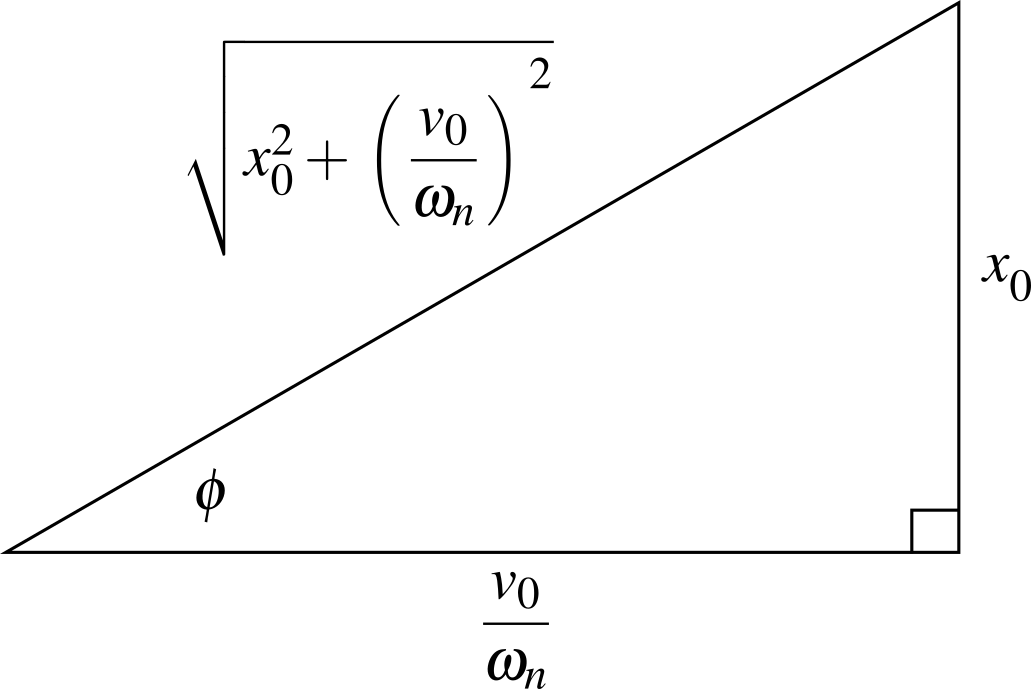
\includegraphics[]{../figures/trigonometric_relationship_undamped_free.png}
				\caption{Trigonometric relationship between the initial conditions ($x_0$ and $v_0$), amplitude $A$, and phase $\phi$ for free vibration of a 1-DOF system.}
				\label{fig:Trigonometric_relationship}
			\end{figure}

		\subsubsection{Special Considerations for No Initial Velocity ($v_0=0$)}
		
			Upon close inspection of the temporal solution in equation \ref{eq:response_simple_harmonic_motion}, it becomes evident that any system without initial velocity (i.e. $v_0=0$) results in an undefined number for $(x_0\omega_\text{n})/v_0$. A solution to this challenge lies in the fact that the limit of tan$^{-1}(x)$ approaches $-\pi/2$ at $-\infty$ and  $\pi/2$ at $\infty$, as depicted in figure \ref{fig:arctan_plot}. Therefore, the solution at $-\infty$ and $\infty$ is undefined, resulting in the expression:
			
			\begin{equation}
				\bigg(\frac{x_0\omega_\text{n}}{v_0}\bigg) = \pm \frac{\pi}{2}, \text{ when } v_0=0
			\end{equation}			
			
			This step is applied in IEEE floating-point arithmetic (IEEE 754) and results in either $\pi/2$ or $\pm \pi/2$ depending on the rounding format used. From the practitioner's side, it becomes important to recognize the situation $v_0=0$ and correct this value as needed. 
			
			\begin{figure}[H]
				\centering
				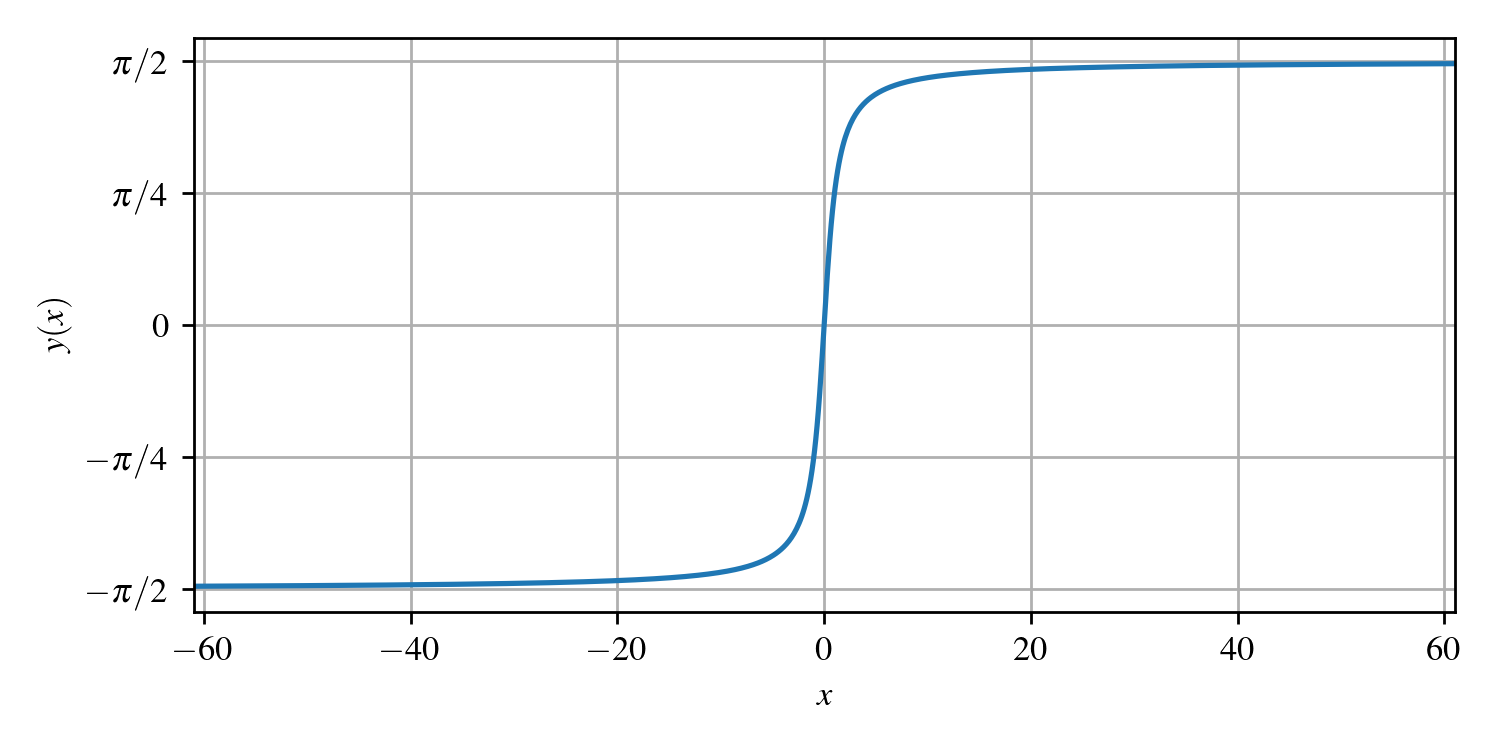
\includegraphics[]{../figures/arctan_plot.png}
				\caption{Response of tan$^{-1}$ (or arctan) for  $x$=-60 to 60 showing that the tan$^{-1}$ is undefined as $x$ approaches $-\infty$ and $\infty$.}
				\label{fig:arctan_plot}
			\end{figure}		
			

			\begin{example}
		
				A vehicle wheel, tire, and suspension can be modeled as an SDOF spring and mass as depicted below: The mass of the wheel and tire is measured to be 300 kg and its frequency of oscillation is observed to be 10 rad/sec. What is the stiffness of the wheel assembly?
				
				\begin{figure}[H]
					\centering
					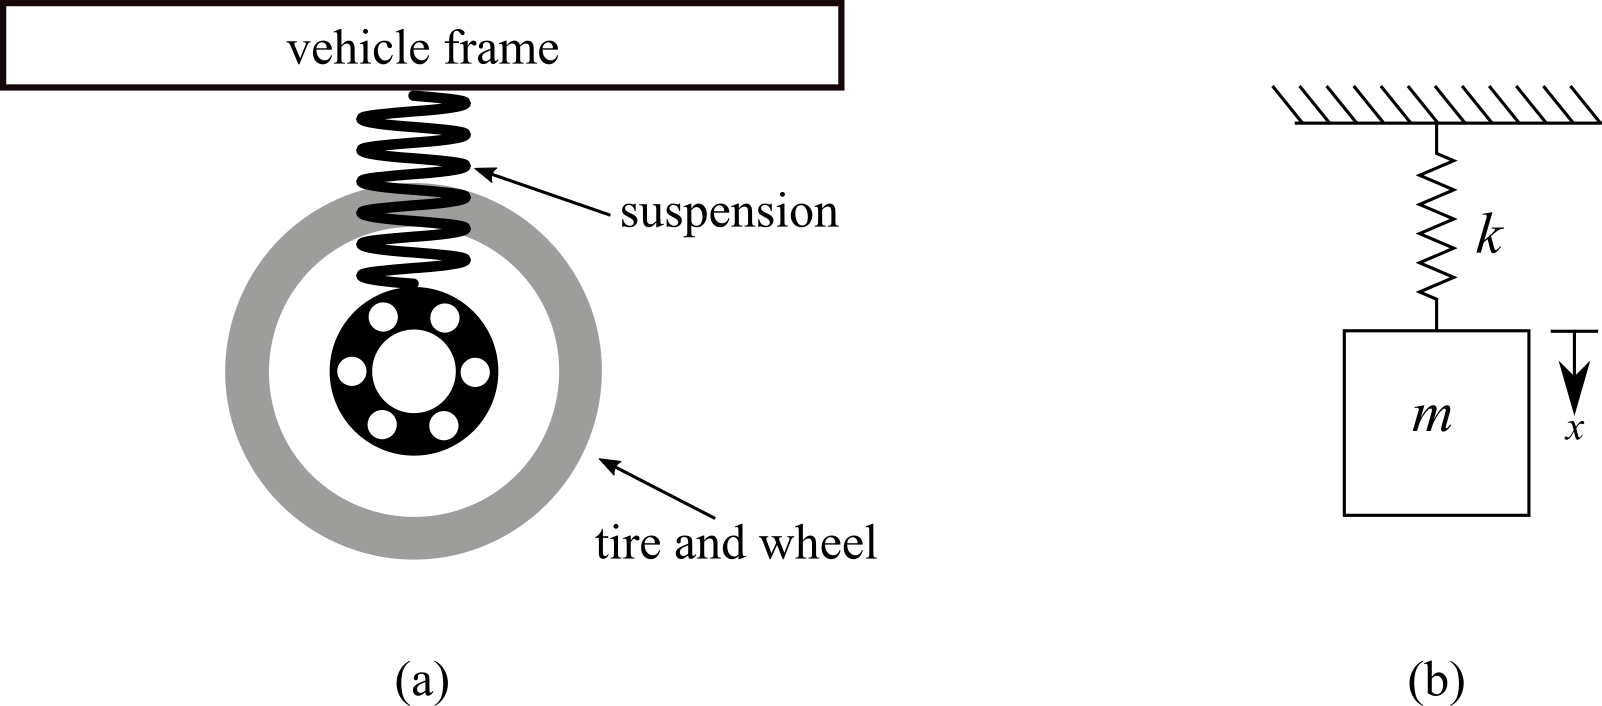
\includegraphics[]{../figures/Vehicle_wheel_undamped.png}
					\caption{Modeling of a vehicle wheel, tire, and suspension showing: (a) Graphical representation; and (b) a spring-mass model.}
					\label{fig:vehicle_wheel_undamped}
				\end{figure}				
				
				\noindent\textbf{Solution:} 
				Considering:
				\begin{equation}
					\omega_\text{n} = \sqrt{\frac{k}{m}}
				\end{equation}
				therefore, $k=m\omega_\text{n}^2=(300$ $\text{kg})(10$ $\text{rad/s})^2=30$ KN/m. Note: radians are a dimensionless quantity and as such the units of  $m\omega_\text{n}^2$ become  $\frac{\rm{kg}}{\rm{s}^2}\cdot\frac{\rm{m}}{\rm{m}}$ where the unit value $\frac{\rm{m}}{\rm{m}}$ is added such that the stiffness of the spring can be expressed as $\frac{\rm{kg}\cdot \rm{m}}{\rm{s}^2}\cdot\frac{1}{\rm{m}}$ = $\frac{\rm{N}}{\rm{m}}$.
			\end{example}
			
			\begin{example}		
				Consider the following 1-DOF system, where $k = 857.8$ N/m and $m=49.2\times10^{-3}$ kg, and calculate the natural frequency in rad/s and Hz. Also, find the period of oscillations and the maximum displacement if the spring is initially displaced $10$ mm with no initial velocity.  	
				\begin{figure}[H]
					\centering
					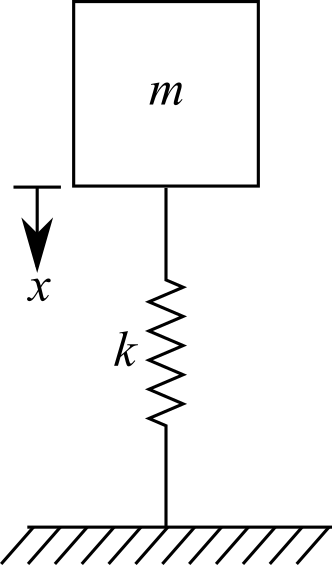
\includegraphics[]{../figures/1-DOF-spring_mass_vertical.png}
					\caption{1-DOF spring-mass system.}
				\end{figure}		
	
				\noindent\textbf{Solution:} 
				\begin{equation}
					\omega_\text{n} = \sqrt{\frac{k}{m}}= \sqrt{\frac{857.8}{49.2\times10^{-3}}} = 132 \hspace{1ex}\text{rad/sec}
				\end{equation}	
				In Hz, this is:
				\begin{equation}
					f_n = \frac{\omega_\text{n}}{2\pi} = 21 \hspace{1ex}\text{Hz}
				\end{equation}						
				The period is:
				\begin{equation}
					T = \frac{2\pi}{\omega_\text{n}} = 0.0476 \hspace{1ex}\text{s}
				\end{equation}					
				The maximum displacement will happen when sin($\omega_\text{n}t+\phi$)$=0$, therefore, the value of $A$ is the maximum displacement. For an undamped system, $	A = \frac{\sqrt{\omega_\text{n}^2x_0^2+v_0^2}}{\omega_\text{n}}$,  
	
	
				\begin{equation}
					A = \frac{\sqrt{\omega_\text{n}^2x_0^2+v_0^2}}{\omega_\text{n}} = \frac{\sqrt{132^2 0.01 ^2+0^2}}{132}=0.01 \hspace{1ex}\text{m}
				\end{equation}
	
			\end{example}

	\subsection{General Solution for Vibrating Systems}

		The EOM for a vibrating system has many solutions and can be expressed in various forms including a general solution. These forms offer different mathematical approaches to solve the same 1-DOF spring-mass system and relate to each other through Euler's equations.
				
		\begin{review}
			Vibration analysis uses complex numbers to solve the EOM's differential equation. In this text the imaginary number is termed $j$ (sometimes referred to as $i$): such that:
			
			\begin{equation}
				j = \sqrt{-1}
			\end{equation}		
			and:	 
			\begin{equation}
				j^2 = -1
			\end{equation}	
			A general complex number, $x$, can be expressed as:
			\begin{equation}
				x=a+bj
			\end{equation}			 	
			here, $a$ is referred to as the real number and $b$ is the imaginary part of the number $x$. Such complex numbers can be represented in the complex plane, also called an Argand plot. The absolute value or modules is defined as $|x|$ presented on the complex plot. 
			
			\begin{figure}[H]
				\centering
				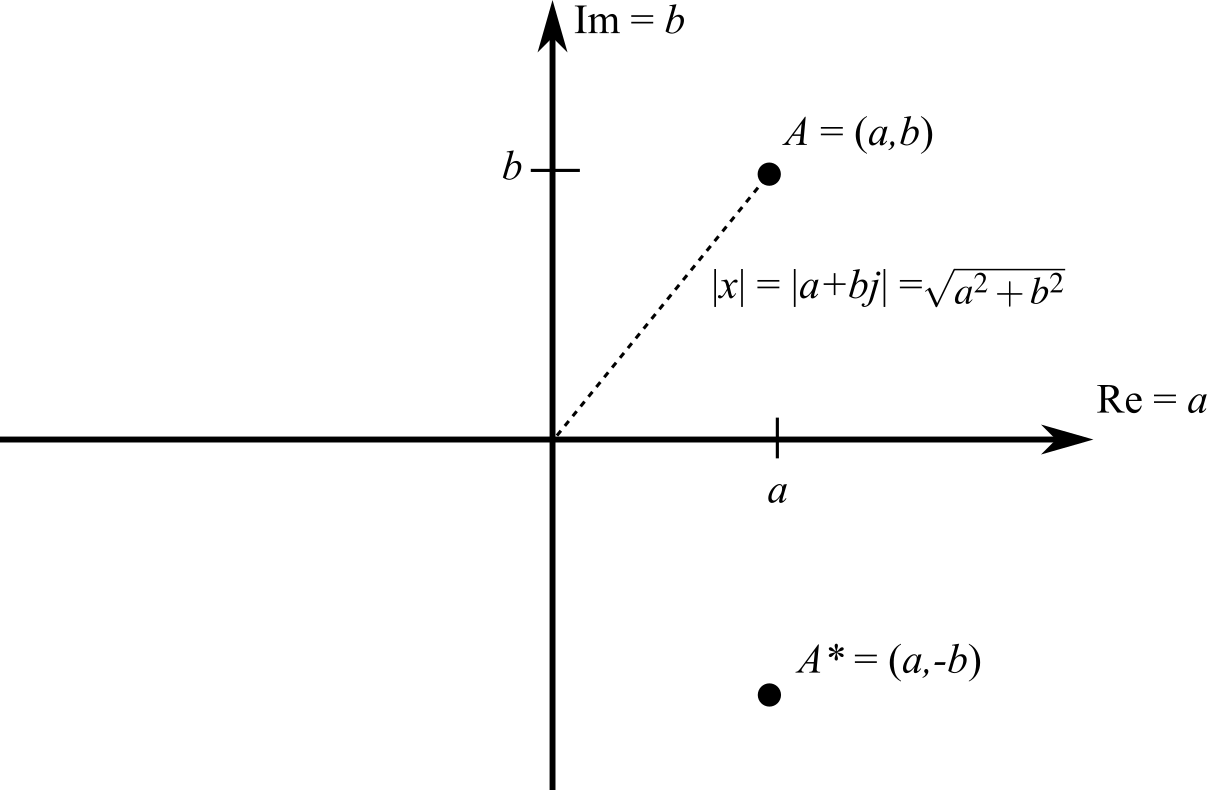
\includegraphics[]{../figures/complex_plane.png}
				\caption{A conjugate pair of numbers ($A$ and $A*$) represented on the complex plane.}
			\end{figure}
					
			$A$ and $A^*$ prime are complex conjugate pairs. In mathematics, the complex conjugate of a complex number is the number with an equal real part and an imaginary part equal in magnitude but opposite in sign. In other words, a conjugate pair is $a + bj$ and $a - bj$.  
			
			\definitionbox{con�ju�gate (adjective)}{Coupled, connected, or related.}

		\end{review}			
		\begin{review}
		
			Euler's (pronounced oy-ler) formula, is a mathematical formula in complex analysis that establishes the fundamental relationship between the trigonometric functions and the complex exponential function. Euler's formula states that for any real number $x$,
			\begin{equation}
				e^{j\psi} = \text{cos}(\psi) + j \text{sin}(\psi)
			\end{equation}		
			where $j=\sqrt{-1}$. This equation can also be expressed as:
			\begin{equation}
				e^{-j\psi} = \text{cos}(\psi) - j \text{sin}(\psi)
			\end{equation}	
			This can be expressed in terms of polar coordinates as:				
			\begin{figure}[H]
				\centering
				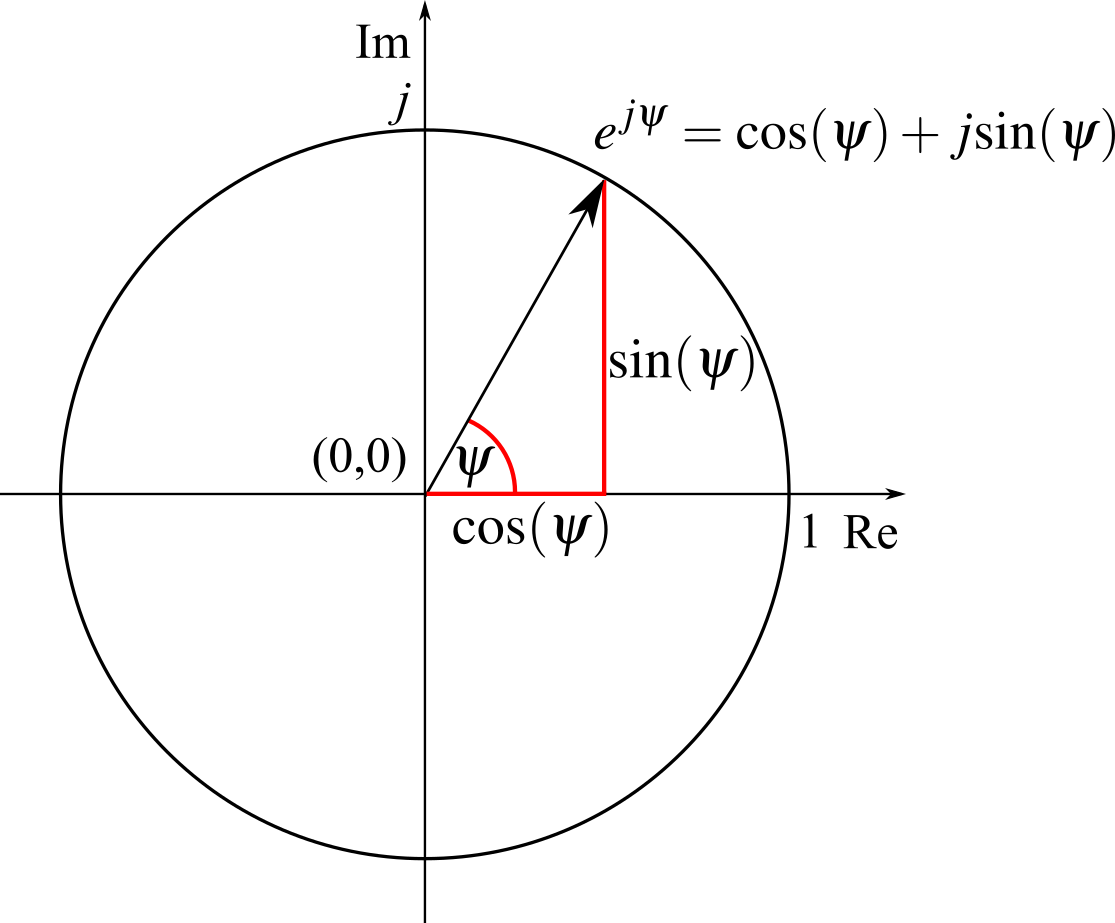
\includegraphics[]{../figures/Eulers_formula.png}
				\caption{Euler's formula illustrated on the unit circle in the complex plane.}
			\end{figure}

			\begin{figure}[H]
				\centering
				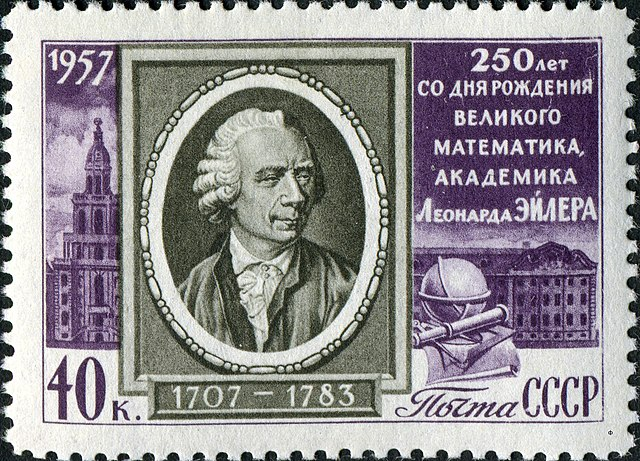
\includegraphics[width=4in]{../figures/Leonhard_Euler}
				\caption{A Soviet Union stamp from 1957 with a Portrait of Leonhard Euler who worked in various branches of the Imperial Russian Academy of Sciences and Imperial court during his lifetime \protect\footnotemark[1].}
			\end{figure}
						
			Euler's formula is named after the Swiss engineer and mathematician Leonhard Euler (1707-1783), who among other things popularized the use of the Greek letter $\pi$ to denote the ratio of a circle's circumference to its diameter, wast the first to use the expression $f(x)$ to denote a function, and correctly defining the base of the natural logarithm $e$; which is now known as Euler's number. While Euler developed ``Euler's formula'' in 1748, it was not used to describe points in a complex for another 50 years when the Danish-Norwegian mathematician and cartographer Caspar Wessel presented to the Danish Academy in 1797  \protect\footnotemark[2].
			

			\footnotetext[1]{Post of the USSR, Public domain, via Wikimedia Commons}  
			\footnotetext[2]{Whittaker, Edmund Taylor, and George Neville Watson. A course of modern analysis: an introduction to the general theory of infinite processes and of analytic functions; with an acount of the principal transcendental functions. University Press, 1927.}  
		
		\end{review}
		
		\subsubsection{Formulating the General Solution for a 1-DOF Spring-Mass System}
			We can also solve the following EOM as an elementary differential equation:
			\begin{equation}
				m\ddot{x}+kx=0
			\end{equation}		
			in a more analytical manner using the theory of elementary differential equations. To do this the form: 
			\begin{equation}
				x(t) = ae^{\lambda t}
			\end{equation}
			is assumed, where $a$ and $t$ are nonzero constants that need to be determined. Using successive differentiation, the assumed solution becomes:
			\begin{equation}
				\dot{x}(t) = \lambda ae^{\lambda t}
			\end{equation}
			and 
			\begin{equation}
				\ddot{x}(t) = \lambda^2 ae^{\lambda t}
			\end{equation}
			therefore, $m\ddot{x}(t) + kx(t) = 0$ becomes:
			\begin{equation}
				m \lambda^2 ae^{\lambda t}  + k ae^{\lambda t} = 0
			\end{equation}
			Next, the above expressions is divide by $ae^{\lambda t}$ to obtain the characteristic equation:
			\begin{equation}
				m \lambda^2 + k = 0
			\end{equation}
			This can be done because $ae^{\lambda t}$ is never zero, therefore, the expression is never divided by zero. The quadratic formula gives us:
			\begin{equation}
				\lambda = \pm \sqrt{-\frac{k}{m}} = \pm \sqrt{\frac{k}{m}}j = \pm \omega_\text{n} j
			\end{equation} 
			remember that $\omega_\text{n} = \sqrt{\frac{k}{m}}$. Notice that the $\pm$ tells us there are two solutions to this problem. So, putting $\lambda$ back into the assumed solution results in two solutions (one positive, one negative):   
			\begin{equation}
				x(t) = a_1e^{+\omega_\text{n} j t}
			\end{equation}
			and 
			\begin{equation}
				x(t) = a_2e^{-\omega_\text{n} j t}
			\end{equation}
			As these solutions only consider, and are only valid for, linear systems; the sum of the solutions is also a solution. This simplification results in:
			\begin{equation}
				x(t) = a_1e^{+\omega_\text{n} j t} + a_2e^{-\omega_\text{n} j t}
			\end{equation}
			where $a_1$ and $a_2$ are constants of integration that scale the unit Euler's vector. The positive and negative values in the exponent indicate that the terms are a conjugate pair.
			
			
			\begin{example}
				Show that $	x(t) = a_1e^{+\omega_\text{n} j t} + a_2e^{-\omega_\text{n} j t}$ is equal to $A\text{sin}(\omega_\text{n} t +\phi)$. \\
				
				\noindent\textbf{Solution:} 
				This equation was derived using Euler's formula and it can be shown that this equation is equivalent to the $A\text{sin}(\omega_\text{n}+\phi)$. To recover the previously assumed solution, the knowledge that $a_1$ and $a_2$ are complex congregate pairs and as such the magnitude can be expressed as $a_1=a_2$ is leveraged. Using Euler's polar notation, $a_1$ and $a_2$ can be expressed as 
				\begin{equation}
					a_1 = a_2 = ae^{j\psi}
				\end{equation}	
				where $a$ and $\psi$ are real numbers, the equation becomes:		
				\begin{equation}
					x(t) = ae^{j(\omega_\text{n} t+\psi)} + ae^{-j(\omega_\text{n} t+\psi)}
				\end{equation}			
				this becomes:
				\begin{equation}
					x(t) = a(e^{j(\omega_\text{n} t+\psi)} + e^{-j(\omega_\text{n} t+\psi)})
				\end{equation}				
				Remembering Euler's equations from before, this becomes:
				\begin{equation}
					x(t) = a\big(\text{cos}(\omega_\text{n} t+\psi) + j \text{sin}(\omega_\text{n} t+\psi) + \text{cos}(\omega_\text{n} t+\psi) - j \text{sin}(\omega_\text{n} t+\psi)\big)
				\end{equation}				
				combining the ``cos'' terms and canceling out the ``sin'' terms this becomes:
				\begin{equation}
					x(t) = 2a \cdot \text{cos}(\omega_\text{n} t+\psi)
				\end{equation}						
				This is equivalent to $	{x}(t) = A\text{sin}(\omega_\text{n} t + \phi)$ considering that $A=2a$ and knowing sin($\phi$) = cos($\phi + \psi$). To expand, this is because the sin and cos are only differentiated by a phase shift. 			
			\end{example}

			
			Next, a general solution for the EOM is obtained. Using the previous solution:
			\begin{equation}
				x(t) = a_1e^{+\omega_\text{n} j t} + a_2e^{-\omega_\text{n} j t}
			\end{equation}			
			we can expand this into the form: 
			\begin{equation}
				x(t) = a_1\big(\text{cos}(\omega_\text{n} t) + j \text{sin}(\omega_\text{n} t)\big) + a_2\big(\text{cos}(\omega_\text{n} t) - j \text{sin}(\omega_\text{n} t)\big)
			\end{equation}
			using trigonometric functions. This equates to:
			\begin{equation}
				x(t) = (a_1+a_2) \cdot \text{cos}(\omega_\text{n} t) + (a_1-a_2)j \cdot \text{sin}(\omega_\text{n} t)
			\end{equation}			
			As $x(t)$ is always real, $A_1$ and $A_2$ can be defined as:
			\begin{equation}
				A_1 = (a_1+a_2)
			\end{equation}		
			and
			\begin{equation}
				A_2 = (a_1-a_2)j
			\end{equation}	
			Lastly, the general solution is written as:
			\begin{equation}
				x(t) = A_1\text{cos}(\omega_\text{n} t) + A_2\text{sin}(\omega_\text{n} t)
			\end{equation}	
			This is the general solution for the EOM ($m\ddot{x}+kx=0$) of the considered oscillating system where $A_1$ and $A_2$ are defined as:
			\begin{equation}
				A = \sqrt{A_1^2+ A_2^2}
			\end{equation}
			and	
			\begin{equation}
				\phi = \text{tan}^{-1}\bigg(\frac{A_1}{A_2}\bigg)
			\end{equation}		
			These are obtained from a trigonometric relationship, similar to that used before:
			\begin{figure}[H]
				\centering
				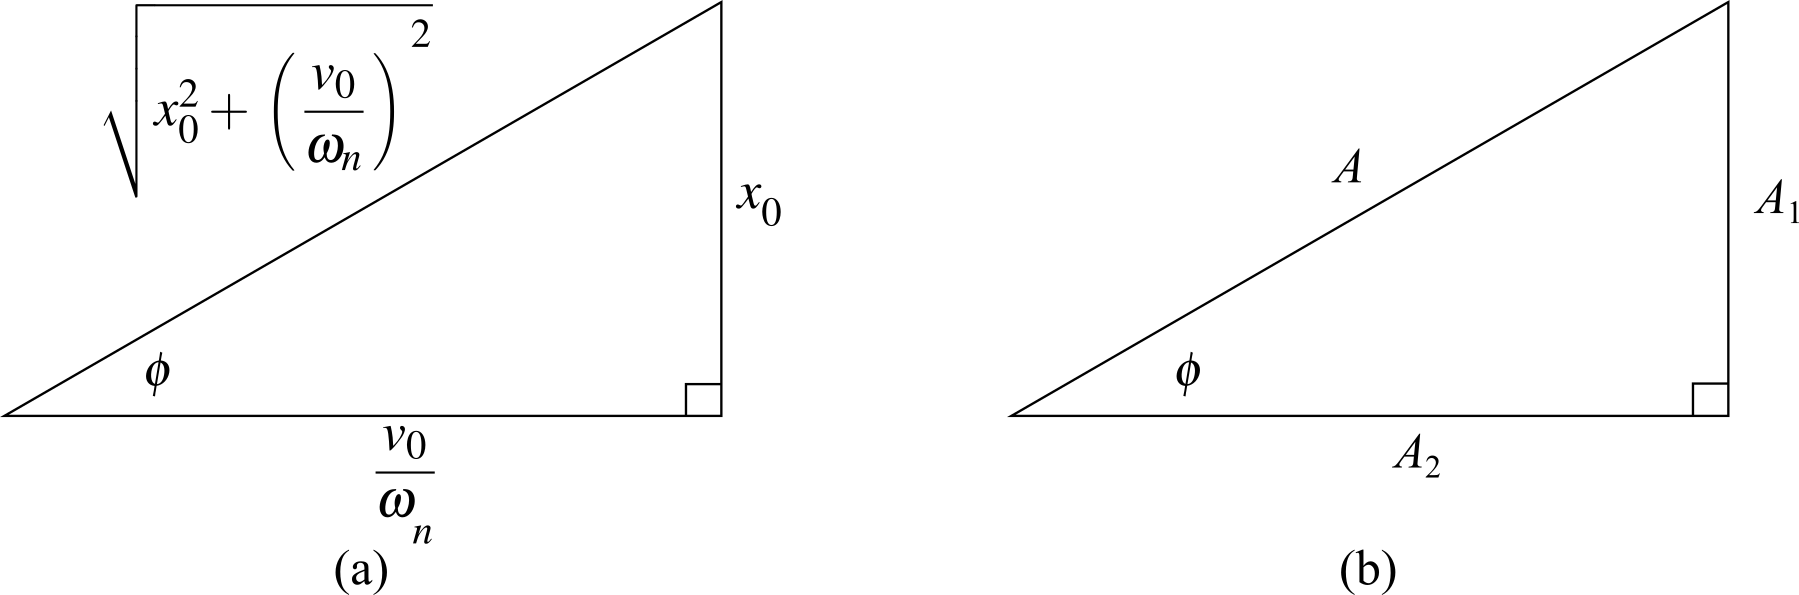
\includegraphics[]{../figures/trigonometric_relationship_undamped_free_general_solution.png}
				\caption{Trigonometric relationship between the initial conditions, amplitude, and phase, for free vibration of a 1-DOF system expressed with: (a) variables for initial conditions; and (b) generic variables $A_{1}$ and $A_{2}$.}
			\end{figure}
			\noindent again, $A$ and $\phi$ are:
			\begin{equation}
				A = \frac{\sqrt{\omega_\text{n}^2x_0^2+v_0^2}}{\omega_\text{n}} = \sqrt{x_0^2+\Bigg(\frac{v_0}{\omega_\text{n}}\Bigg)^2}
			\end{equation}
			\begin{equation}
				\phi = \text{tan}^{-1}\bigg(\frac{x_0\omega_\text{n}}{v_0}\bigg)
			\end{equation}		


			\begin{example}			
				Using the general solution: 
				\begin{equation}
					x(t) = A_1\text{cos}(\omega_\text{n} t) + A_2\text{sin}(\omega_\text{n} t)
				\end{equation}			
				Calculate the values of $A_1$ and $A_2$ in terms of their initial conditions $x_0$ and $v_0$.
				
				\noindent\textbf{Solution:} Knowing the following for $x$ and $\dot{x}$:
				\begin{equation}
					x(t) = A_1\text{cos}(\omega_\text{n} t) + A_2\text{sin}(\omega_\text{n} t)
				\end{equation}	
				\begin{equation}
					\dot{x}(t) = -A_1\omega_\text{n}\text{sin}(\omega_\text{n} t) + A_2\omega_\text{n}\text{cos}(\omega_\text{n} t)
				\end{equation}	
				Now apply the initial conditions, $x(0)=0$ and $v(0)=0$, this yields:
				\begin{equation}
					x(0) = x_0 = A_1
				\end{equation}	
				\begin{equation}
					\dot{x}(0)= v_0  =  A_2\omega_\text{n}
				\end{equation}
				Solving for $A_1$ and $A_2$ shows us:
				\begin{equation}
					A_1 = x_0 \text{, and } A_2 = \frac{v_0}{\omega_\text{n}}
				\end{equation}
				thus:
				\begin{equation}
					x(t) = x_0\text{cos}(\omega_\text{n} t) + \frac{v_0}{\omega_\text{n}}\text{sin}(\omega_\text{n} t)
				\end{equation}				
			\end{example}

		\subsubsection{Solution of 1-DOF System in Three Forms}
			Form one, for $m\ddot{x} + kx =0$ subject to nonzero initial conditions can be written as:  		
			\begin{equation}
				x(t) = a_1e^{+\omega_\text{n} j t} + a_2e^{-\omega_\text{n} j t}
			\end{equation}	
			where $a_1$ and $a_2$ are complex terms. Form two is:
			\begin{equation}
				{x}(t) = A\text{sin}(\omega_\text{n} t + \phi)
			\end{equation}
			while form three is:
			\begin{equation}
				x(t) = A_1\text{cos}(\omega_\text{n} t) + A_2\text{sin}(\omega_\text{n} t)
			\end{equation}	
			where $A$, $\phi$, $A_1$, and $A_2$, are all real-valued constants. Each set of constants can be related to each other by:
			\begin{align}
				\label{eq:A_1_and_A_2}
				A = \sqrt{A_1^2+ A_2^2} & \hspace{1.5cm} \phi = \text{tan}^{-1}\bigg(\frac{A_1}{A_2}\bigg) \\
				A_1 = (a_1+a_2) & \hspace{1.5cm} A_2 = (a_1-a_2)j \\
				a_1 = \frac{A_1-A_2j}{2} & \hspace{1.5cm} a_2 = \frac{A_1+A_2j}{2}
			\end{align}
			Which follow from trigonometric identities and Euler's formula. 


	
	\subsection{Damping}
	
	
		The response of a spring-mass system predicts that a system will oscillate indefinitely. However, we know that this is not true from observing real-world solutions. So based on real-world observations and mathematical conveniences, we need to add a term that will remove ``energy'' from the system with time. To do this the idea of the ideal dashpot is introduced. A linear dashpot is diagrammed in figure \ref{fig:linear_dashpot} and is a mechanical device that resists motion via viscous friction and therefore converts the mechanical energy of the system into thermal energy that is dissipated.
		
		\begin{figure}[H]
			\centering
			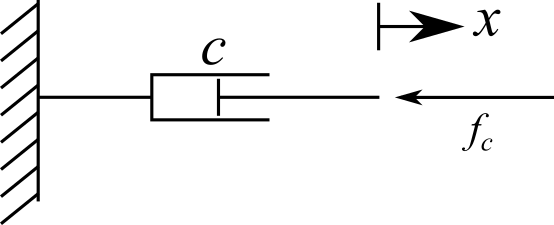
\includegraphics[]{../figures/linear_dashpot.png}
			\caption{Schematic of a liner dashpot showing the damping force ($f_c$) acting in the opposite direction of the displacement ($x$).}
			\label{fig:linear_dashpot}
		\end{figure}
		
		Just as spring forms a physical model of the cause vibration, through its storage and release of energy, a dashpot (sometimes called a damper) forms a physical model for dissipating energy. Dashpots create a resisting or damping force that acts opposite to the direction of travel (as annotated in figure \ref{fig:linear_dashpot}) and is proportional to the velocity. Therefore, the damping forces $f_c$ can be computed as:
		\begin{equation}
			f_c = c \dot{x}
		\end{equation}
		the constant $c$, called the damping coefficient, has the units of kg/s. Dashpots are a mathematical representation of viscous dampers installed in automobiles, aircraft, structures, and other mechanical devices. However, all systems have inherent damping not just systems with physical dampers. The spring-mass system can be used as a representation of real-world systems with inherent damping as demonstrated by the rubber engine mount depicted in figure \ref{fig:rubber_engine_mount}.
		
		
		\begin{figure}[H]
			\centering
			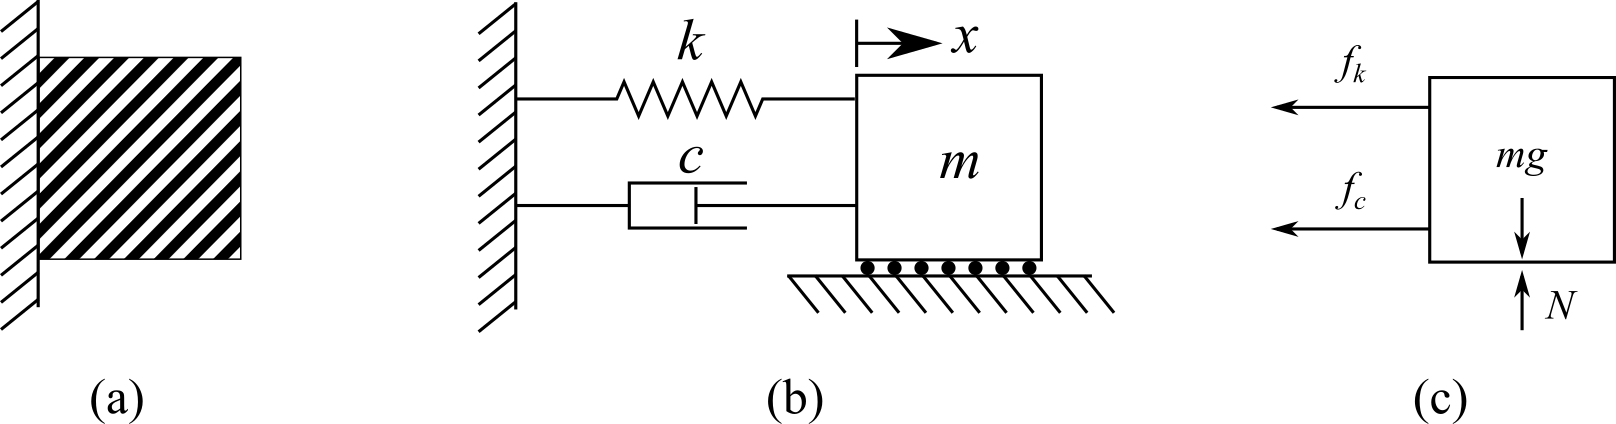
\includegraphics[]{../figures/engine_mount_model.png}
			\caption{Modeling of a rubber engine mount as an spring-dashpot-mass model showing (a) the rubber engine mount; (b) idealized model of the rubber month; and (c) the FBD of the idealized model}
			\label{fig:rubber_engine_mount}
		\end{figure}

		Depending on the amount of damping present in a system, the temporal response of the system will represent itself in various ways, as represented in figure \ref{fig:damping_cases}. To reiterate, an undamped case will oscillate around the equilibrium and does not decay. If a limited amount of damping is present in a system it will oscillate around the equilibrium and slowly decay with time to the equilibrium position, this is termed underdamped. If an excessive amount of damping is present, the system will not oscillate but decay directly to the equilibrium position, this is termed the overdamped case. Lastly, there exists a special case that results in the system converging as quickly as possible to the equilibrium position without oscillations; this case is termed the critically damped case. Furthermore, the amount of damping required to obtain a critically damped system is the damping value that the underdamped and overdamped cases for a specific system. To recap, the key types of damping are:
		
		\begin{itemize}
			\item \textbf{Undamped} - Oscillates around the equilibrium and does not decay.
			\item \textbf{Underdamped} - Oscillates around the equilibrium and slowly decays and is the most common case.
			\item \textbf{Overdamped} - Does not pass the equilibrium position and is a simple decay with no oscillation.
			\item \textbf{Critically damped} - provides the quickest approach to zero amplitude for a damped oscillator.
		\end{itemize}
		
		
		\begin{figure}[H]
			\centering
			\includegraphics[]{../figures/damping_cases.png}
			\caption{Temporal responses for the three types of damping: underdamped, overdamped, and critically damped.}
			\label{fig:damping_cases}
		\end{figure}
			
		\subsubsection{Modeling Vibrating Systems with Damping}
				
			The spring-mass system of Chapter 1 can be expanded to a spring-dashpot-mass system that considers the damping component of the system. A mathematical model of the spring-dashpot-mass system can be developed for the case present in figure \ref{fig:1-DOF-mass_horizontal_damping_FBD}. Using the FBD for the system, it can conclude that the EOM for this system:
			\begin{figure}[H]
				\centering
				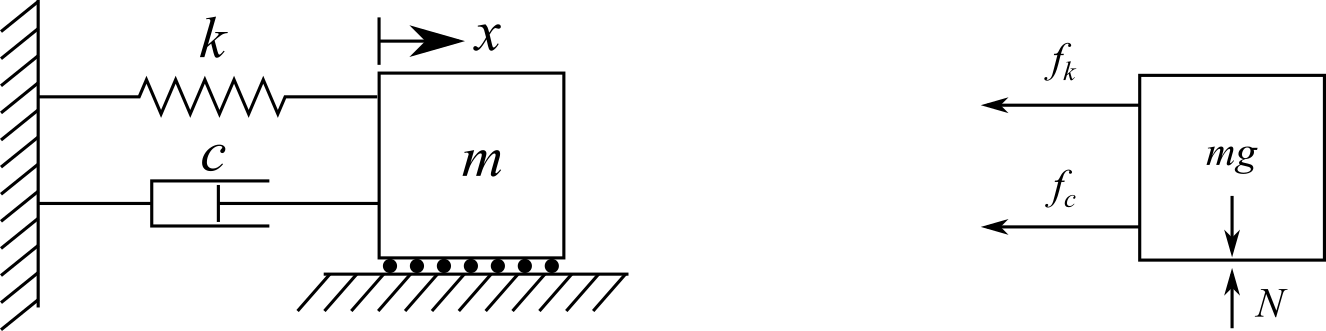
\includegraphics[]{../figures/1_DOF_spring_dashpot_mass_horizontal_FBD.png}
				\caption{Spring-dashpot-mass model showing: (a) a schematic of the system; and (b) the FBD of the system. }
				\label{fig:1-DOF-mass_horizontal_damping_FBD}
			\end{figure}			
			\noindent is:
			\begin{equation}
				m\ddot{x}(t) = - f_c - f_k
			\end{equation}
			Rearranging into standard form and concerting forces into parameters $c$ and $k$ results in:
			\begin{equation}
				m\ddot{x}(t) + c \dot{x}(t) + kx(t) = 0
			\end{equation}
			This system is subject to the same initial conditions as before, $x(0) = x_0$ and $\dot{x}(0) = v_0$. Again, choosing to model it this way for convinces, so let's solve it in a similar manner to the EOM without damping. Again, assume the solution:
			\begin{equation}
				x(t) = ae^{\lambda t}
			\end{equation}
			here, $a$ and $t$ are nonzeros constants that need to be determined.  Using successive differentiation, we get:
			\begin{equation}
				\dot{x}(t) = \lambda ae^{\lambda t}
			\end{equation}
			and 
			\begin{equation}
				\ddot{x}(t) = \lambda^2 ae^{\lambda t}
			\end{equation}
			therefore, $m\ddot{x} + c\dot{x} + kx = 0$ becomes:
			\begin{equation}
				m \lambda^2 ae^{\lambda t}  +c\lambda ae^{\lambda t} + k ae^{\lambda t} = 0
			\end{equation}
			Now we divide by $ae^{\lambda t}$ to obtain the \textbf{characteristic equation}:
			\begin{equation}
				m \lambda^2 + c\lambda + k = 0
			\end{equation}
			We can do this because $ae^{\lambda t}$ is never zero, therefore, we never divide by zero. The quadratic formula gives us:
			\begin{equation}
				\lambda_{1,2} = \frac{-c \pm \sqrt{c^2-4km}}{2m}  = \frac{-c}{2m} \pm \frac{1}{2m}\sqrt{c^2-4km}
			\end{equation}
			Some key points from this equation:
			\begin{itemize}
			\item The $\pm$ tells us there are two solutions to this problem
			\item if $c^2-4km<0$, system is Underdamped, solutions are complex conjugate pairs 
			\item if $c^2-4km=0$, system is critically damped, solutions are equal negative real numbers 
			\item if $c^2-4km>0$, system is Overdamped, solutions are distinct negative real numbers 
			\end{itemize}
			From this, we can see that $c^2-4km=0$ is a special value, let us define a value for $c$ that will give us this critical damping number. We will call it the \textbf{critical damping coefficient} ($c_{\text{cr}}$). So setting the equation as:
			\begin{equation}
				c_{\text{cr}}^2-4km = 0
			\end{equation}
			giving us: 
			\begin{equation}
				c_{\text{cr}}^2 = 4km
			\end{equation}		
			next, we can derive the function:
			\begin{equation}
				c_{\text{cr}} = 2\sqrt{km} = 2\bigg(\frac{\sqrt{m}}{\sqrt{m}}\bigg)\sqrt{km} = 2m\omega_\text{n}
			\end{equation}			
			remember that $\omega_\text{n} = \sqrt{\frac{k}{m}}$ for an undamped system. Next, we generate a non-dimensional number ($\zeta$), pronounced `zeta' that will allow us to distinguish between different types of damping. $\zeta$ is called the \textbf{critical damping ratio}.
			\begin{equation}
				\zeta = \frac{c}{c_{\text{cr}}} = \frac{c}{2\sqrt{km}} = \frac{c}{2m\omega_\text{n}}
			\end{equation}				
			Now if we put the $\zeta$ back into the characteristic equation and resolve using the quadratic equation we get: 
			\begin{equation}
				\lambda_{1,2} = -\zeta\omega_\text{n} \pm \omega_\text{n} \sqrt{\zeta^2-1}
			\end{equation}
			From this equation, it becomes clear that $\zeta$ determines whether the roots are complex or real, this, in turn, determines the nature of the response of the structure. Listing the possible responses we get:
			\begin{table}[h!]
				\centering
				\begin{tabular}{lccc}
					\toprule
					damping case & critical damping ratio & radicand & solutions  \\ \midrule
					under damped &  $0<\zeta<1$ & $c^2-4km<0$ & complex conjugate pairs \\
					critically damped & $\zeta=1$ & $c^2-4km=0$ & equal negative real numbers \\
					over damped & $1<\zeta$  & $c^2-4km>0$ & distinct negative real numbers \\ \bottomrule
				\end{tabular}
			\end{table}
			For each damping case, we will have a different solution to the problem. 
					
		\subsubsection{Modeling Underdamped Motion}
		
 			In the case that $0<\zeta<1$, a complex conjugate pair of roots are the solutions to the characteristic equation after pulling out a $\sqrt{-1}$:
			\begin{equation}
				\lambda_{1} = -\zeta\omega_\text{n} + \omega_\text{n} \sqrt{1-\zeta^2}j
			\end{equation} 			
			and:
			\begin{equation}
				\lambda_{2} = -\zeta\omega_\text{n} - \omega_\text{n} \sqrt{1-\zeta^2}j
			\end{equation} 
			Where the $j$ is pulled out because:
			\begin{equation}
				\sqrt{1-\zeta^2}j = \sqrt{(1-\zeta^2)(-1)} = \sqrt{\zeta^2-1}
			\end{equation} 							
			Next, let us ``arbitrarily'' define:
			\begin{equation}
				\omega_\text{d} = \omega_\text{n}\sqrt{1-\zeta^2}
			\end{equation} 	
			where $\omega_\text{d}$ is the \textbf{damped natural frequency}. Therefore, the equations become:
			\begin{equation}
				\lambda_{1} = -\zeta\omega_\text{n} + \omega_\text{d}j
			\end{equation} 			
			and:
			\begin{equation}
				\lambda_{2} = -\zeta\omega_\text{n} - \omega_\text{d}j
			\end{equation} 	
			Again, we have two solutions to a linear problem, so we can combine these into one solution and insert $\lambda$ into the assumed solution $ae^{\lambda t}$ to obtain:
			\begin{equation}
				x(t) = a_1e^{-\zeta\omega_\text{n}t + \omega_\text{d}tj} + a_2e^{-\zeta\omega_\text{n}t - \omega_\text{d}tj} 
			\end{equation} 			
			where $a_1$ and $a_2$ are complex valued constants. This can now be simplified into:	
			\begin{equation}
				x(t) = e^{-\zeta\omega_\text{n}t}(a_1e^{\omega_\text{d}tj} + a_2e^{-\omega_\text{d}tj}) 
			\end{equation} 

			Using Euler's equations, (same as before) and choosing:
			\begin{equation}
				A_1=(a_1-a_2)j
			\end{equation} 	
			and
			\begin{equation}
				A_2=(a_1+a_2)
			\end{equation} 		
			Note that the $A_1$ and $A_2$ defined here are the reverse of those defined in Eq.~\ref{eq:A_1_and_A_2}. This is done to allow the general form to be in the same format as before, however, assuming the same $A_1$ and $A_2$ would not change the final solution expressed below. The general form of this solution is then:
			\begin{equation}
				x(t) = e^{-\zeta\omega_\text{n}t}\big(A_1\text{sin}(\omega_\text{d}t) + A_2\text{cos}(\omega_\text{d}t)\big)
			\end{equation} 	
			Recall that for undamped 1-DOF systems we showed 
			\begin{equation}
				x(t) = A\text{sin}(\omega_\text{n}t + \phi) = A_1\text{sin}(\omega_\text{n}t) + A_2\text{cos}(\omega_\text{n}t)
			\end{equation} 	
			As $e^{-\zeta\omega_\text{n}t}$ accounts for the damping, our current solution becomes:
			\begin{equation}
				x(t) = Ae^{-\zeta\omega_\text{n}t}\text{sin}(\omega_\text{d}t + \phi) 
			\end{equation} 		

			Now that we have $x$ and $\dot{x}$, we can solve for the boundary conditions $x_0$ and $v_0$ by setting $t=0$, we get:
			\begin{equation}
				x(0)=x_0 = A\text{sin}(\phi) 
			\end{equation} 			
			and taking the directive of $x(t)$ using the product rule (fg)'= f'g+fg', we get:
			\begin{equation}
				\dot{x}(t) = -\zeta\omega_\text{n}Ae^{-\zeta\omega_\text{n}t}\text{sin}(\omega_\text{d}t + \phi) + Ae^{-\zeta\omega_\text{n}t}\omega_\text{d}\text{cos}(\omega_\text{d}t + \phi) 
			\end{equation} 
			\begin{equation}
				\dot{x}(0) =v_0= -\zeta\omega_\text{n}A\text{sin}(\phi) + A\omega_\text{d}\text{cos}(\phi) 
			\end{equation} 
			a simplification can be made to the prior equation by letting $A=x_0/\text{sin}(\phi)$. This gives us the equation:
			\begin{equation}
				\dot{x}(0) =v_0= -\zeta\omega_\text{n}\bigg(\frac{x_0}{\text{sin}(\phi)}\bigg)\text{sin}(\phi) + \bigg(\frac{x_0}{\text{sin}(\phi)}\bigg)\omega_\text{d}\text{cos}(\phi) 
			\end{equation} 			
			that can be simplified to:
			\begin{equation}
				\dot{x}(0) = v_0 = -\zeta\omega_\text{n}x_0 + x_0\omega_\text{d}\text{cot}(\phi) 
			\end{equation} 	
			The above equation related $v_0$ to $\phi$ using terms that are known for a giving system ($\zeta,\, \omega_\text{n},\, x_0 \text{, and }\omega_\text{d} $). Therefore, this expression can be used to solve for $\phi$:
			\begin{equation}
				\text{cot}(\phi) = \frac{v_0 +\zeta\omega_\text{n}x_0}{x_0\omega_\text{d}} 
				\label{eq:underdamped_phi}
			\end{equation} 	
			and as $\tan(\phi) = 1/\text{cot}(\phi)$: 
			\begin{equation}
				\phi = \tan^{-1}\Bigg(\frac{x_0\omega_\text{d}}{v_0+\zeta\omega_\text{n}x_0}\Bigg)
			\end{equation} 				
			Thereafter, we can solve for $A$ considering the fact that we sent $A=x_0/\text{sin}(\phi)$. Using the trigonometric relationship between expressed in equation \ref{eq:underdamped_phi} and visualized in figure \ref{fig:trigonometric_relationship_underdamped}:
			\begin{figure}[H]
				\centering
				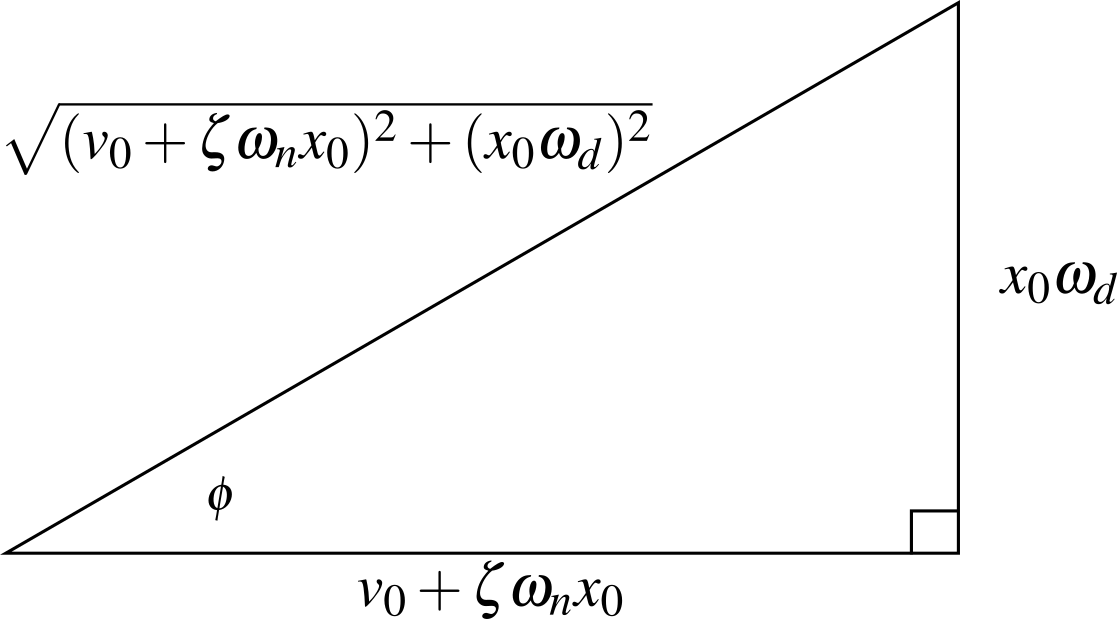
\includegraphics[]{../figures/trigonometric_relationship_underdamped.png}
				\caption{Trigonometric relationship between the initial conditions ($x_0$ and $v_0$), amplitude $A$, and phase $\phi$ for underdamped motion of a 1-DOF system.}
				\label{fig:trigonometric_relationship_underdamped}
			\end{figure}
			\noindent we show that $\text{sin}(\phi)$ can be expressed as: 
			\begin{equation}
				\text{sin}(\phi) = \frac{x_0\omega_\text{d}}{\sqrt{(v_0+\zeta\omega_\text{n}x_0)^2 + (x_0\omega_\text{d})^2}}
			\end{equation} 	
			and applying $A=x_0/\text{sin}(\phi)$ we get:
			\begin{equation}
				A = \frac{\sqrt{(v_0+\zeta\omega_\text{n}x_0)^2 + (x_0\omega_\text{d})^2}}{\omega_\text{d}} = \sqrt{x_0^2 + \Bigg( \frac{v_0 + \zeta \omega_\text{n} x_0}{\omega_\text{d}}\Bigg)^2}
			\end{equation} 								
			Finally, collecting all of our important equations:
			\begin{itemize}
			\item Critical damping coefficient: $c_{\text{cr}} = 2\sqrt{km} = 2m\omega_\text{n}$
			\item Damping ratio: $	\zeta = \frac{c}{c_{\text{cr}}} = \frac{c}{2\sqrt{km}} = \frac{c}{2m\omega_\text{n}}$
			\item Damped natural frequency: $\omega_\text{d} = \omega_\text{n}\sqrt{1-\zeta^2}$
			\item Solution for underdamped system: $x(t) = Ae^{-\zeta\omega_\text{n}t}\text{sin}(\omega_\text{d}t + \phi)$, where: \begin{align*}
						A = \frac{\sqrt{(v_0+\zeta\omega_\text{n}x_0)^2 + (x_0\omega_\text{d})^2}}{\omega_\text{d}} & \hspace{1.5cm} \phi = \text{tan}^{-1}\Bigg(\frac{x_0\omega_\text{d}}{v_0+\zeta\omega_\text{n}x_0}\Bigg) 
						\end{align*}
			\end{itemize}

			\begin{figure}[H]
				\centering
				\includegraphics[]{../figures/under_damped_various_initial_conditions.png}
				\caption{Four example responses for an underdamped 1-DOF system  ($\zeta=0.142$) with various initial conditions.}
			\end{figure}

		\begin{example}				
			Consider the following 1-DOF system, where $k = 857.8$ N/m, $c=7.8$ kg/s, and $m=49.2\times10^{-3}$ kg, calculate the damped frequency in rad/s and Hz. What damping case is this system?  
			\begin{figure}[H]
				\centering
				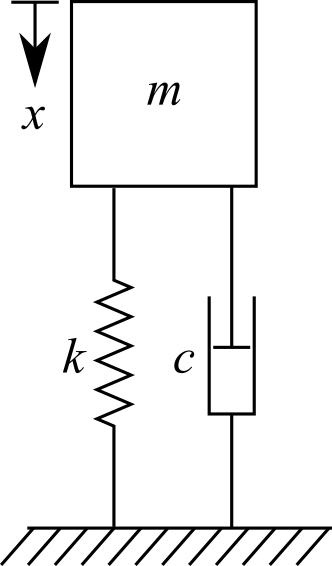
\includegraphics[]{../figures/1_DOF_spring_dashpot_mass_vertical.png}
				\caption{1-DOF spring-dashpot-mass system.}
			\end{figure}		

			\noindent\textbf{Solution:} 
			
			Calculate the undamped frequency:
			\begin{equation}
				\omega_\text{n} = \sqrt{\frac{k}{m}}= \sqrt{\frac{857.8}{49.2\times10^{-3}}} = 132 \hspace{1ex}\text{rad/s}
			\end{equation}	
			The systems critical damping value:
			\begin{equation}
				c_{\text{cr}} = 2\sqrt{km}= 2\sqrt{k = 857.8 \cdot 49.2\times10^{-3}} = 12.993 \hspace{1ex}\text{kg/s}
			\end{equation}		
			And the critical damping ratio:
			\begin{equation}
				\zeta = \frac{c}{c_{\text{cr}}} = \frac{7.8}{12.993} = 0.600
			\end{equation}				
			This can also be expressed as 60\% damped, this is an underdamped system, and the system will oscillate. Now we can calculate the damped frequency:
			\begin{equation}
				\omega_\text{d} = \omega_\text{n}\sqrt{1-\zeta^2} = \omega_\text{n}\sqrt{1-0.600^2} = 105.6 \hspace{1ex}\text{rad/s}
			\end{equation}		
			Therefore, the system oscillates at 105.6 rad/sec or 16.81 Hz
		\end{example}

		\begin{example}
			For a damped one DOF system where $m$, $c$, and $k$ are known to be $m$ = 1 kg, $c$ = 2 kg/s, and $k$ = 10 N/m. Calculate the value of $\zeta$ and $\omega_\text{n}$. Is the system overdamped, underdamped, or critically damped?	

			\noindent\textbf{Solution:} 
						
			The natural frequency is calculated as
			\begin{equation}
				\omega_\text{n} = \sqrt{\frac{k}{m}} = \sqrt{\frac{10}{1}} = 3.16 \hspace{1ex} \text{rad/s}
			\end{equation}
			The damping can be calculated as:
			\begin{equation}
				\zeta = \frac{c}{2\omega_\text{n} m} = \frac{2}{2\Big(\sqrt{\frac{10}{1}}\Big)(1)} = \frac{1}{\sqrt{10}} = 0.316 
			\end{equation}
			So the damped natural frequency is equal to:
			\begin{equation}
				\omega_\text{d} = \omega_\text{n}\sqrt{1-\zeta^2} =  \sqrt{10}\sqrt{1-\bigg(\frac{1}{\sqrt{10}}\bigg)^2} = 3 \hspace{1ex} \text{rad/s}
			\end{equation}			
			As $0<\zeta<1$ the system is underdamped. 			
		\end{example}

		\begin{example}
			Figure~\ref{fig:rubber_mounted_mass_with_spring} shows an industrial device consisting of a mass isolated from its fixtures by two rubber dampers and an offset spring with an angle $\alpha$. Provide an estimate of the system's damped natural frequency in the vertical direction.	Assume the rubber dampers add damping and only negligible stiffness to the system and that the spring is long enough such that the angles remain constant. 	
			\begin{figure}[H]
				\centering
				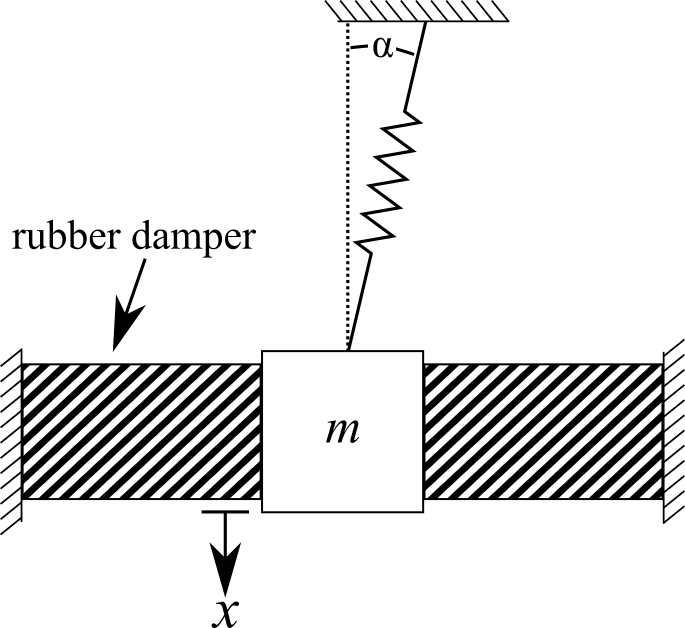
\includegraphics[]{../figures/rubber_mounted_mass_with_spring.png}
				\caption{Industrial device (mass) connected to a fixed point with a rubber damper and spring at an angle.}
				\label{fig:rubber_mounted_mass_with_spring}
			\end{figure}
	
			\noindent\textbf{Solution:} 
			
			First and foremost, we need to develop a mass-spring-dashpot representation of the system. This is presented in what follows:
			
			\begin{figure}[H]
				\centering
				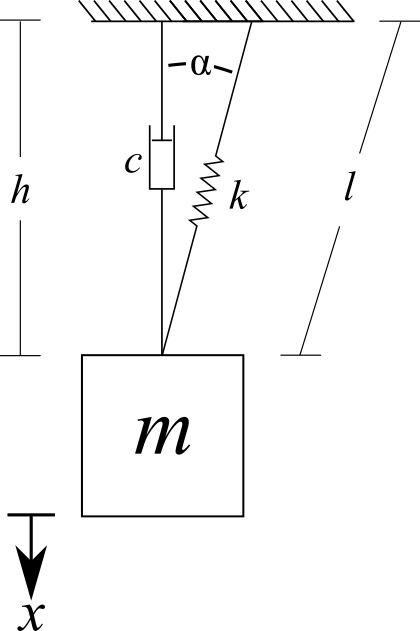
\includegraphics[]{../figures/rubber_mounted_mass_with_spring_spring_dashpot_system.png}
				\caption{Mass-spring-dashpot representation of the industrial system represented if figure \ref{fig:rubber_mounted_mass_with_spring}.}
			\end{figure}
				
			where the damping in the vertical direction provided by the rubber damper is modeled as a dashpot in the vertical direction. As we only want an estimate of the frequency, the assumption that the is small and as such $\alpha$ of the displaced state is equal $\alpha$ of the equilibrium state. This leads to the FBD for the equilibrium  and displaced states:
			
			\begin{center}
				equilibrium position \hspace{4cm} displaced position ``x''
			\end{center}
			\begin{figure}[H]
				\centering
				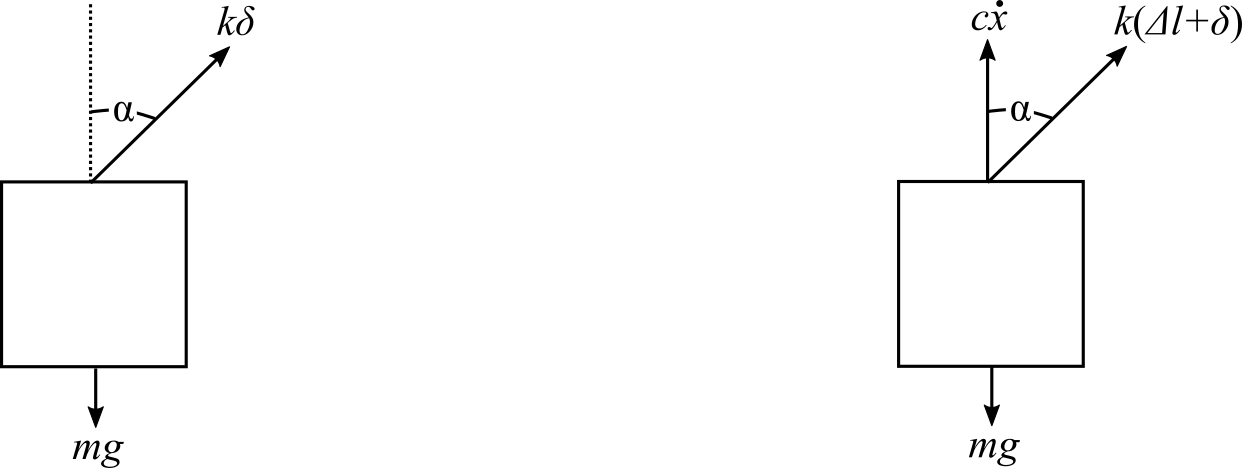
\includegraphics[]{../figures/rubber_mounted_mass_with_spring_FBD.png}
			\end{figure}
			The equation for the equilibrium state is:
			\begin{equation*}
				\downplus \sum F_x = mg -k\delta\text{cos}(\alpha) =0
			\end{equation*}
			and in the displaced state:
			\begin{equation*}
				\downplus \sum F_x = mg - c\dot{x}-k\text{cos}(\alpha)(\Delta l+\delta)
			\end{equation*}
			Applying Newton's second law and combining these equations yields:
			\begin{equation*}
				m\ddot{x} + c\dot{x} + k \Delta l \text{cos}(\alpha) =0
			\end{equation*}	
			Looking at the triangles formed by the dashpot and spring it can be shown that:
			\begin{equation*}
				 \cos(\alpha) = h/l = x/\Delta l  
			\end{equation*}			
			As we assumed the displacement is small and $\alpha$ remains unchanged. Therefore the prior equation becomes: 
			\begin{equation*}
				m\ddot{x} + c\dot{x} + k \Delta l \frac{x}{\Delta l} = 0
			\end{equation*}	
			This simplifies to the ``normal'' EOM for a 1-DOF system: 
			\begin{equation*}
				m\ddot{x} + c\dot{x} + k x  = 0
			\end{equation*}				
			Therefore, once the values for the system are measured the system's damped natural frequency in the vertical direction can be estimated as		
			\begin{equation*}
				\boxed{\omega_\text{d} = \omega_\text{n}\sqrt{1-\zeta^2}}
			\end{equation*}
		\end{example}	
	
		\begin{vibration_case_study}
			Epoxy-based damping is used in the automotive field to reduce vehicle noise and vibration harshness (NVH). This passive form of damping is essential for increasing comfort in modern light-wight vehicles. 
			
		\begin{figure}[H]
		\centering
		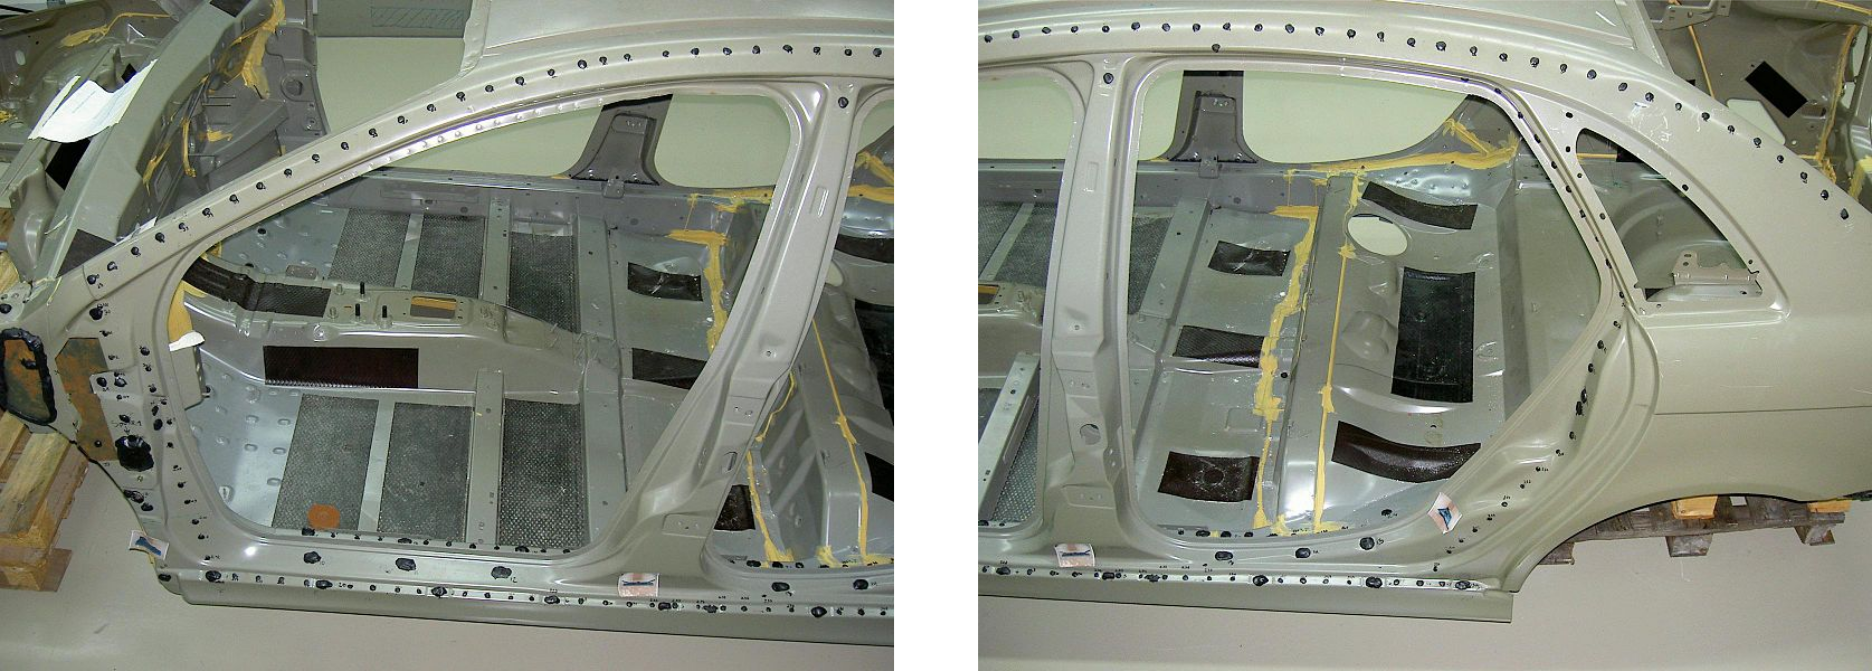
\includegraphics[width=6in]{../figures/automotive_epoxy_damping}
		\caption{Experimental modal analysis of an automotive (Jaguar) body in white, typically done to reduce vehicle noise and vibration harshness.\protect\footnotemark[1]}
			\footnotetext[1]{Cjp24, CC BY-SA 3.0 $<$https://creativecommons.org/licenses/by-sa/3.0$>$, via Wikimedia Commons.}
	\end{figure}		
			
	
		
			
			
		\end{vibration_case_study}
			
		\subsubsection{Modeling Overdamped Motion}
			
			In the case of overdamped systems, $1<\zeta$, the solutions for $\lambda$ are distinct real roots that are written as:
			\begin{equation}
				\lambda_{1} = -\zeta\omega_\text{n} - \omega_\text{n} \sqrt{\zeta^2-1}
			\end{equation} 			
			and:
			\begin{equation}
				\lambda_{2} = -\zeta\omega_\text{n} + \omega_\text{n} \sqrt{\zeta^2-1}
			\end{equation} 
			The solution for the EOM using the assumed solution then becomes:
			\begin{equation}
				x(t) = e^{-\zeta\omega_\text{n}t}(a_1e^{-\omega_\text{n} t \sqrt{\zeta^2-1}} + a_2e^{+\omega_\text{n} t \sqrt{\zeta^2-1}}) 
			\end{equation}
			This equation represents a non-oscillating response of the system. Again, $a_1$ and $a_2$ are solved for using known boundary conditions $x_0$ and $v_0$ such that:
			\begin{align}
				a_1 &= \frac{-v_0+\Big(-\zeta+\sqrt{\zeta^2-1}\Big)\omega_\text{n} x_0}{2\omega_\text{n}\sqrt{\zeta^2-1}} \\ 
				a_2 &= \frac{v_0+\Big(\zeta+\sqrt{\zeta^2-1}\Big)\omega_\text{n} x_0}{2\omega_\text{n}\sqrt{\zeta^2-1}}
			\end{align}				
			Typical responses for an overdamped system with various initial conditions are shown below in figure~\ref{fig:Over_damped_various_initial_conditions}.
			\begin{figure}[H]
				\centering
				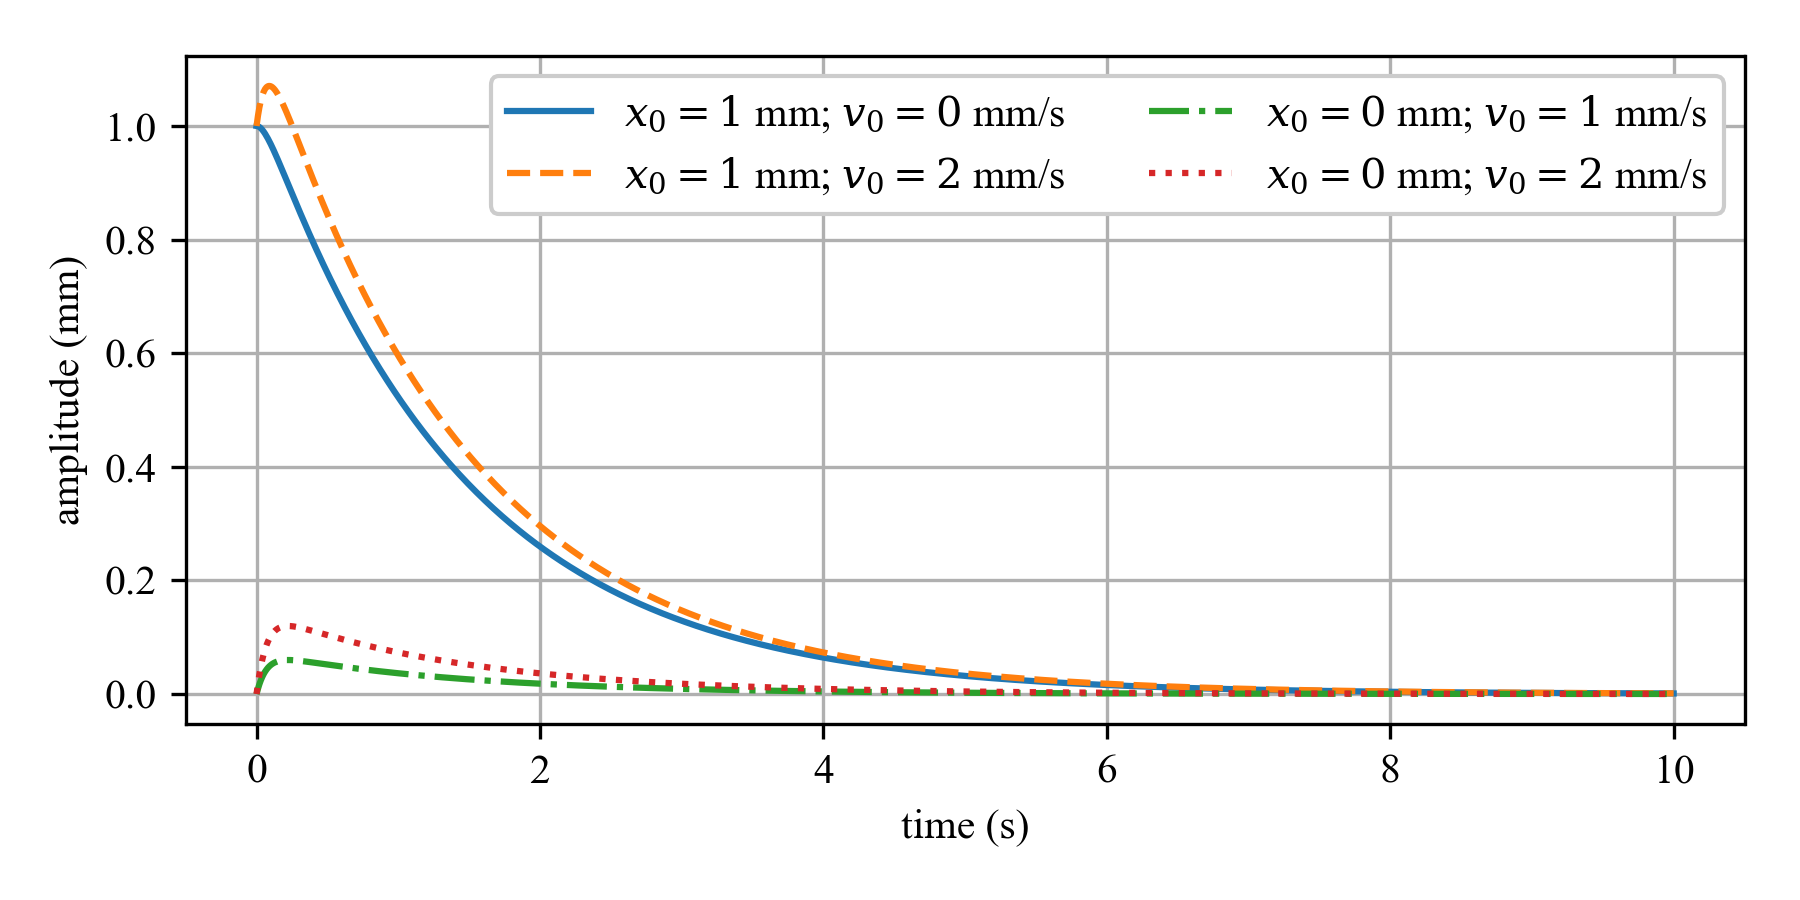
\includegraphics[]{../figures/Over_damped_various_initial_conditions.png}
				\caption{Four example responses for an overdamped 1-DOF system ($\zeta=2.371$) with various initial conditions.}
				\label{fig:Over_damped_various_initial_conditions}
			\end{figure}

		\subsubsection{Modeling Critically Damped Motion}			

			In the case of critically damped systems, $\zeta=1$, the solutions for $\lambda$ will be equal negative real numbers, therefore from before:
			\begin{equation}
				\lambda_{1,2} = -\zeta\omega_\text{n} \pm \omega_\text{n} \sqrt{\zeta^2-1}
			\end{equation}
			We get:
			\begin{equation}
				\lambda_{1} = \lambda_{2} = -\omega_\text{n}
			\end{equation} 			
			Because both solutions ($a_1$ and $a_2$) are the same, we multiply the second solution by $t$ so the solution for a critically damped system is in the same form as before. The solution for the EOM using the assumed solution then becomes:
			\begin{equation}
				x(t) = a_1e^{-\omega_\text{n}t} + a_2te^{-\omega_\text{n}t} 
			\end{equation} 
			This simplifies into:			
			\begin{equation}
				x(t) = (a_1+a_2t) e^{-\omega_\text{n}t} 
			\end{equation}
			This equation represents a non-oscillating response of the system. Again, $a_1$ and $a_2$ are solved for using known boundary conditions $x_0$ and $v_0$ such that:
			\begin{align}
				a_1 &= x_0 \\ 
				a_2 &= v_0+\omega_\text{n}x_0
			\end{align}				


		\subsubsection{Standard Form of the EOM}
			
			The EOM for a damped 1-DOF system is written in a ``standard form'' in which the effect of the damping ratio and natural frequencies are more obvious. To get to the standard form, the normal form of the EOM:
			\begin{equation}
				m\ddot{x} + c \dot{x} + kx = 0
			\end{equation}
			is divided by what the constant terms associated with the acceleration term. In this example, this is $m$. Dividing every term by $m$ yields: 
			\begin{equation}
				\ddot{x} + \frac{c}{m}\dot{x} + \frac{k}{m}x = 0
			\end{equation}		
			Numerical manipulations can be undertaken to get the coefficients of the velocity and displacement terms into coefficients that more clearly express the characteristics of the vibrating system:
			\begin{equation}
				\ddot{x} + 2\zeta\omega_\text{n}\dot{x} + \omega_\text{n}^2x = 0
			\end{equation}	

		\begin{example}

		An engine valve assembly is depicted in figure \ref{fig:engine_valve} where $J$ is the inertia caused by the right-hand side of the rocker arm. Derive an analytical solution for the natural frequency of the rocker arm. Use the assumptions sin($\theta$) = $\theta$ and cos($\theta$) = 1.
		
			\begin{figure}[H]
				\centering
				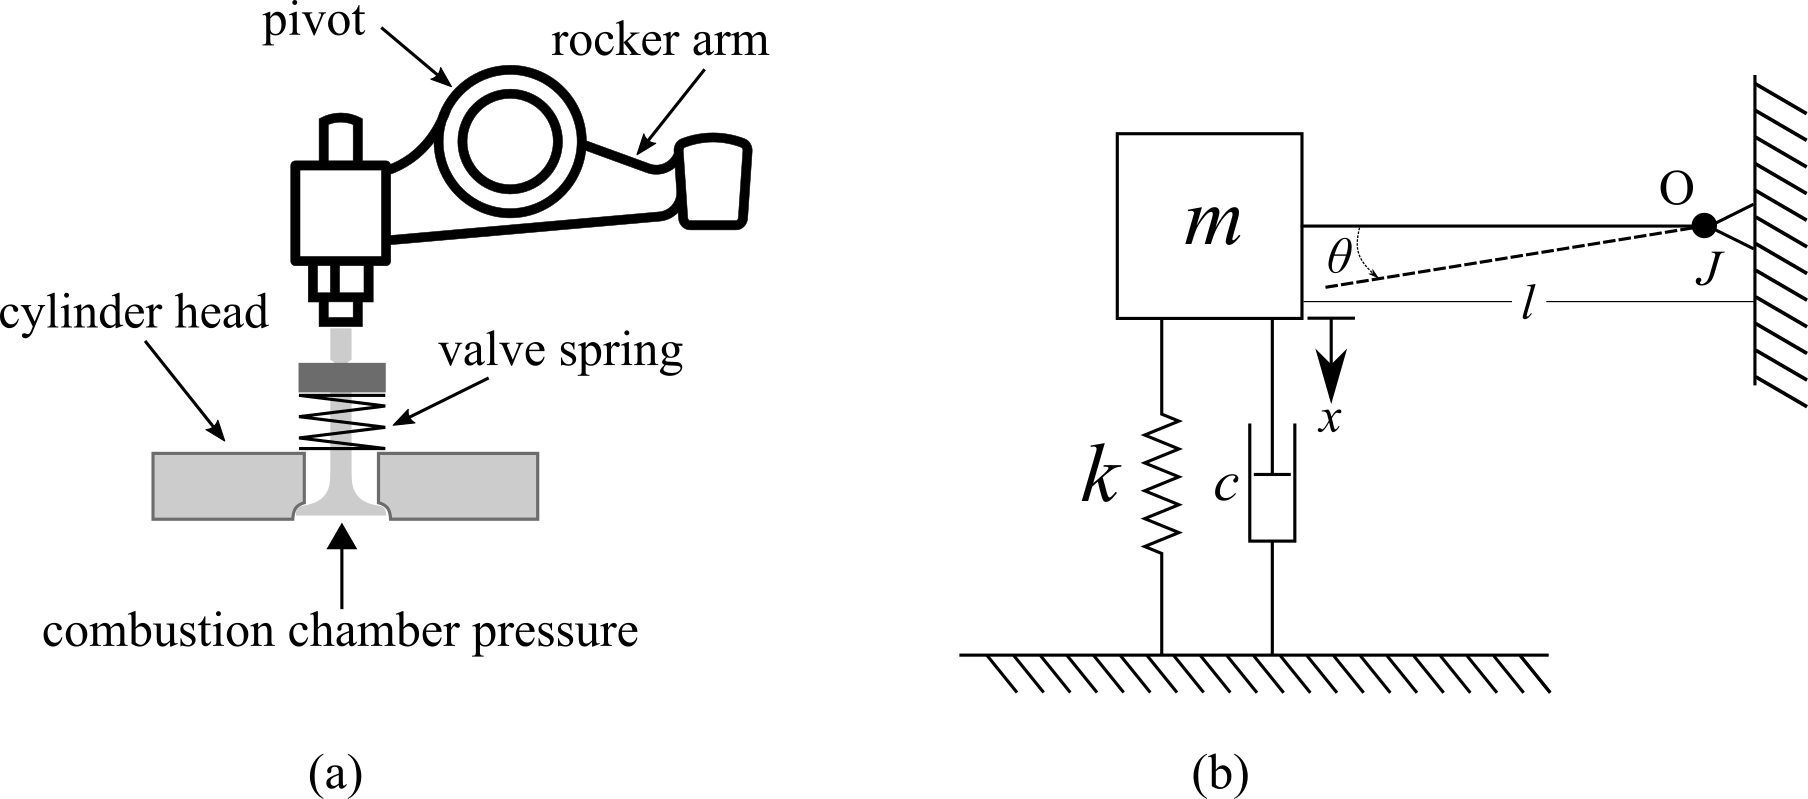
\includegraphics[]{../figures/engine_valve.png}
				\caption{Rocker arm assembly of an internal combustion engine showing: (a) a diagram of the system and; (b) the FBD of the system.}
				\label{fig:engine_valve}
			\end{figure}
			
		\noindent\textbf{Solution:} 
		
		Taking the sum of the moments about $O$ and considering the inertia caused by the right-hand side of the rocker arm, $J$, the FBDs can be written as: 
		\begin{center}
			equilibrium position \hspace{4cm} displaced position ``x''
		\end{center}
		\begin{figure}[H]
			\centering
			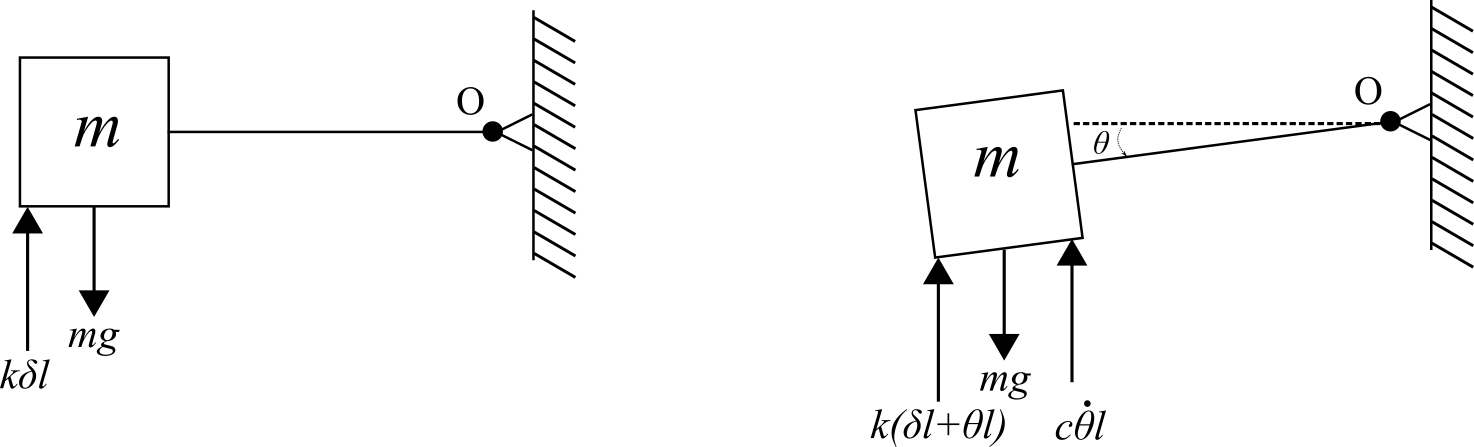
\includegraphics[]{../figures/engine_valve_FBD.png}
		\end{figure}
		The equation for the equilibrium state is:
		\begin{equation*}
			\curveplus \sum M_o = mgl -k l^2 \delta =0
		\end{equation*}
		and in the displaced state:
		\begin{equation*}
			\curveplus \sum M_o = mgl -k l^2 \delta -k l^2 \theta -c l^2\dot{\theta} =0
		\end{equation*}
		Applying Newton's second law and combining these equations yields:
		\begin{equation}
			(J+ml^2)\ddot{\theta} +cl^2\dot{\theta} + kl^2 \theta = 0
		\end{equation}	
		Therefore, the standard form of the EOM is:
		\begin{equation}
			\ddot{\theta} + \frac{cl^2}{J+ml^2}\dot{\theta} + \frac{kl^2 }{J+ml^2}\theta  = 0
		\end{equation}	
		Results in the following analytical solution for the natural frequency:
		\begin{equation}
			\omega_\text{n} = \sqrt{\frac{kl^2 }{J+ml^2}} \text{ rad/s}
		\end{equation}	
							
		\end{example}	


		\begin{vibration_case_study}
			
			On August 17\textsuperscript{th}, 2009 Turbine 2 of the hydroelectric power station of the Sayano-Shushenskaya Dam near Sayanogorsk in Russia failed catastrophically. The failure flooded the turbine hall and collapsed the ceiling. Killing 75 people, many of whom were in the turbine hall to celebrate the anniversary of the plant's general director.  Turbines of the type used at Sayano-Shushenskaya are designed to have high efficiency but a very narrow working band. When they operate outside the designed working band, they vibrate due to the pulsation of water flow and water strokes. These vibrations degrade the turbine over time. 
			
			Turbine 2 had experienced excessive vibrations for a long time, ever since its installation in 1979. Through the early '80s several issues were fixed, along with substantial repairs in 2000 and 2005.  In July 2009 the turbine again exceeded the allowed vibration specification but stayed in operation. Over the years, the operating staff simply came to accept the higher level of vibration. The final government report stated that the accident was caused by turbine vibrations which led to fatigue damage in a turbine mount. 
			
			\begin{figure}[H]
				\centering
				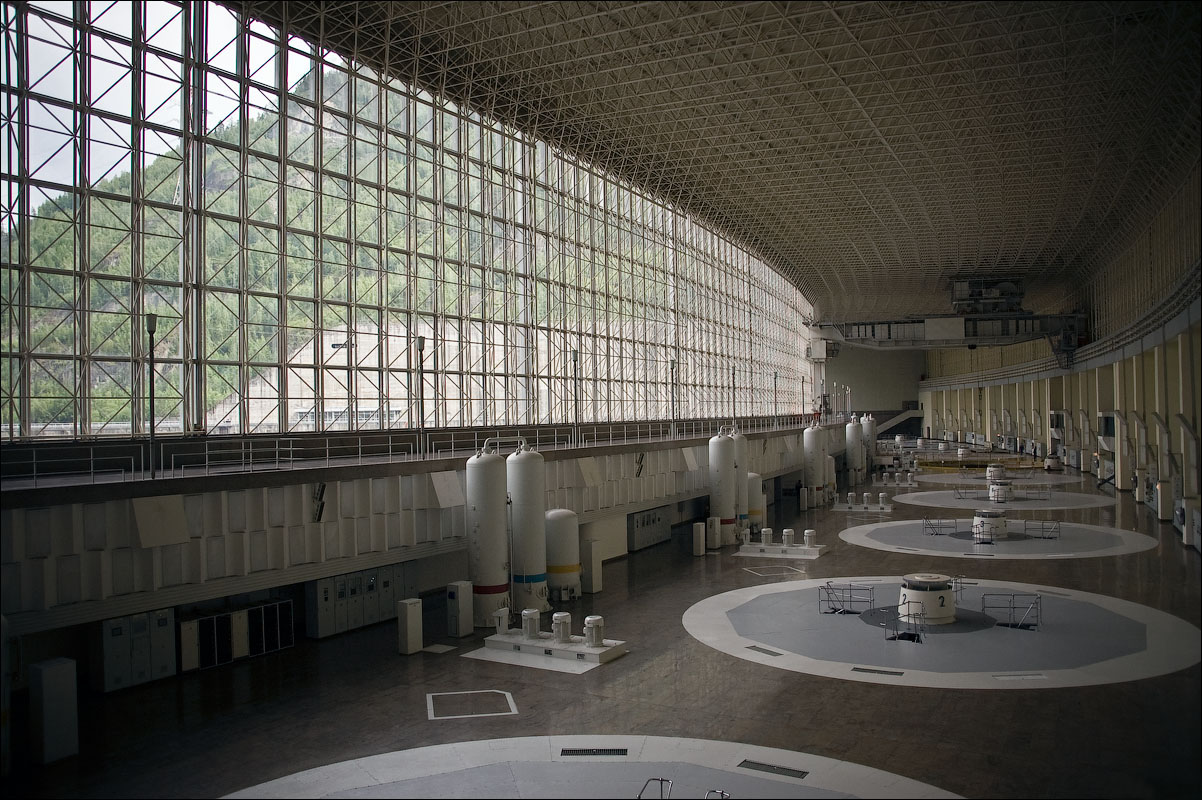
\includegraphics[width=4in]{../figures/Sayano-Shushenskaya_HPS_-_generator_hall}
				\caption{Sayano Shushenskaya's turbine hall before the accident where turbine 2 (the turbine that failed) is in the foreground of the image. \protect\footnotemark[1]}
			\end{figure}

			\begin{figure}[H]
				\centering
				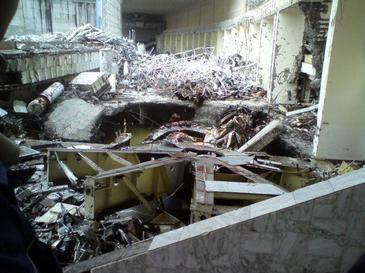
\includegraphics[width=4in]{../figures/Sayano-Shushenskaya_HPS_-_generator_hall_post-accident}
				\caption{Sayano Shushenskaya's turbine hall after the accident. \protect\footnotemark[2] \bl{} }
			\end{figure}
			
%			\begin{otherlanguage*}{russian}
%			????? ?? ??????? ?????
%			\end{otherlanguage*}

			\footnotetext[1]{4044415 \foreignlanguage{russian}{Russian: Andrey Korzun} English:  Andrey Korzun, CC BY-SA 3.0 $<$https://creativecommons.org/licenses/by-sa/3.0$>$, via Wikimedia Commons}
			\footnotetext[2]{The original source of this photograph is believed to be Jaffaa, a user of forums.drom.ru, who uploaded it on August 17, 2009, a few hours after the accident. This image is a faithful digitization of a unique historic image, and the copyright for it is most likely held by the person who created the image or the agency employing the person. It is believed that the use of this image may qualify as fair use under the copyright law of the United States.}

		\end{vibration_case_study}

 
	
%	4044415 ???????:  ?????? ?????? English:  Andrey Korzun, CC BY-SA 3.0 <https://creativecommons.org/licenses/by-sa/3.0>, via Wikimedia Commons
	
		\subsection{Logarithmic Decrement}
			
			For a vibrating system, the mass ($m$) and stiffness ($k$) can be measured using scales and static deflection tests. However, the damping coefficient ($c$) is a more difficult quantity to determine. From $k$ and $m$ we can compute the natural frequency ($\omega_\text{n}$) and the critical damping coefficient ($c_\text{cr}$). Therefore, knowing that the critical damping ratio ($\zeta$) is defined as:
			\begin{equation}
				\zeta = \frac{c}{c_{\text{cr}}} = \frac{c}{2\sqrt{km}} = \frac{c}{2m\omega_\text{n}}
			\end{equation}				
			if we calculate $\zeta$, we can obtain $c$ for the system of interest. This is made possible because $c_\text{cr}$ can be calculated from $k$ and $m$. Observing the temporal response for the underdamped system, 
			\begin{figure}[H]
				\centering
				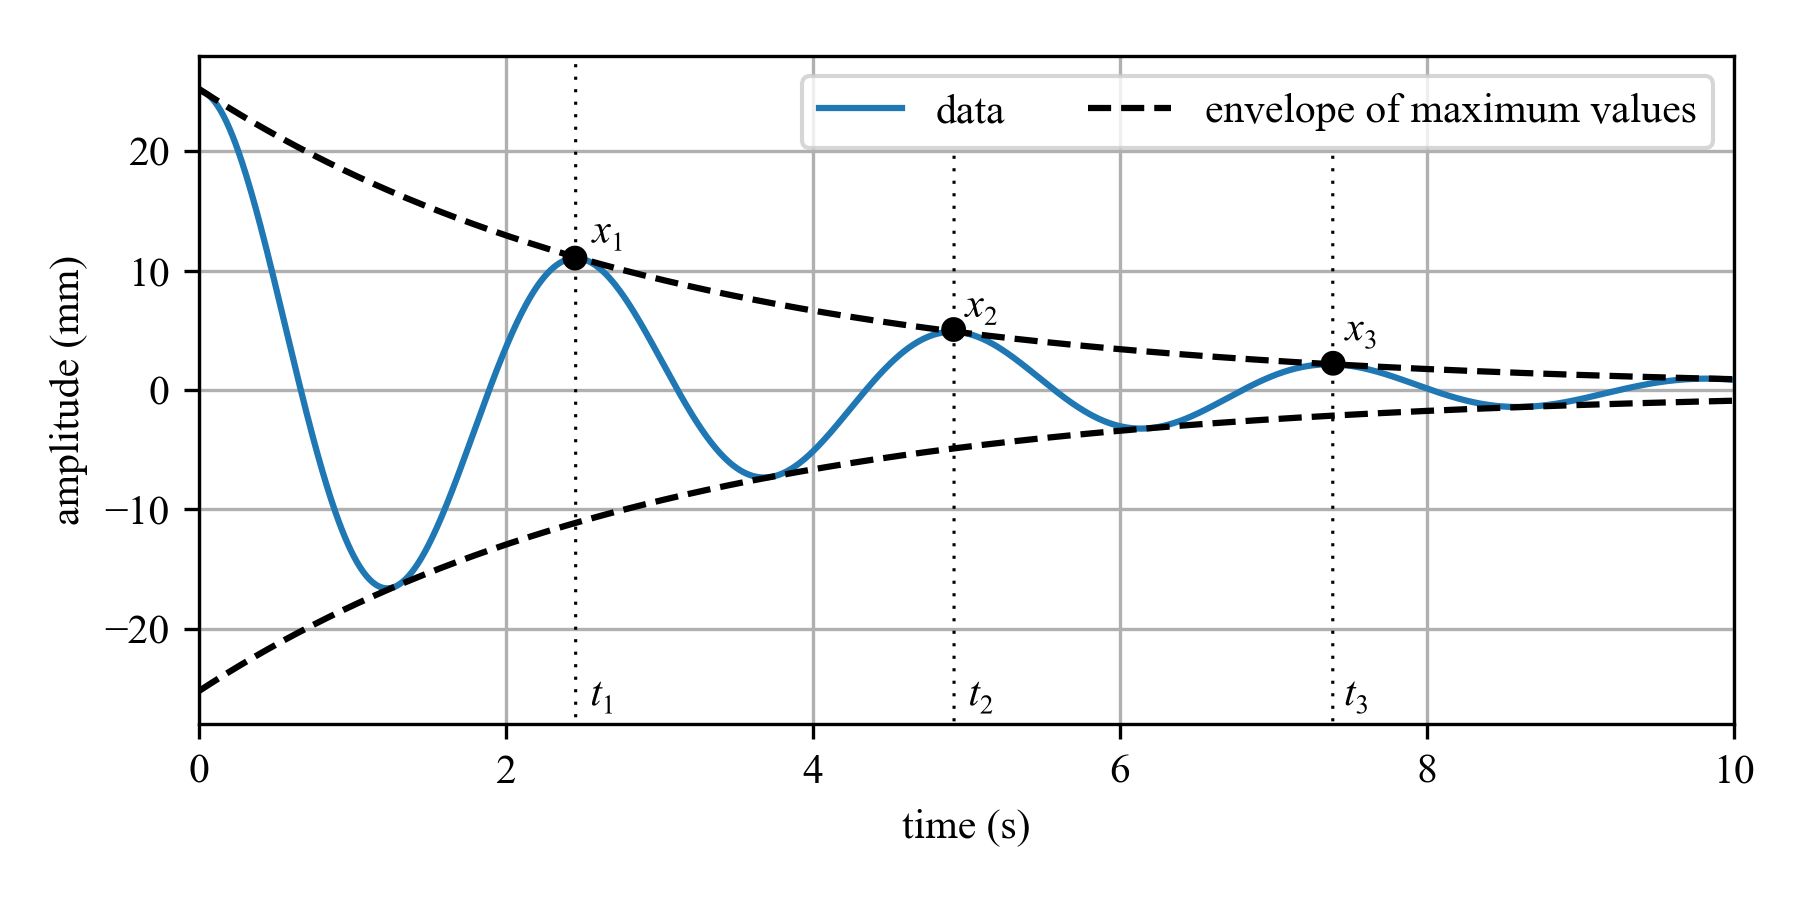
\includegraphics[]{../figures/Logarithmic_decrement.png}
				\caption{Measuring the peak displacement points in an experimental system with decay caused by damping.}
			\end{figure}
			
			\noindent we mark three points of maximum amplitude, $x_1$, $x_2$, and $x_3$ that happen at $t_1$, $t_2$, and $t_3$, respectively. Considering displacement values for the first two points $x_1$ and $x_2$, separated by a complete period ($T$).  Knowing that one cycle is $2 \pi$, the time period for this complete cycle is given by:
			\begin{equation}
				t_2-t_1 = \frac{2\pi}{\omega_\text{d}} = \frac{2\pi}{\omega_\text{n}\sqrt{1-\zeta^2}}
			\end{equation}				
			where $\omega_\text{d}$ is the damped natural frequency. This is the time period ($T$) of damped oscillations. If we derive an equation for the values of the peaks, also called the envelope of maximum values, we get: 
			\begin{equation}
				x_{\text{peaks}} = Ae^{-\zeta\omega_\text{n}t} 
			\end{equation} 		
			Knowing that the system is underdamped, $A$ can be solved for using the initial conditions $x_0$ and $v_0$, therefore: 
			\begin{equation}
				A = \frac{\sqrt{(v_0+\zeta\omega_\text{n}x_0)^2 + (x_0\omega_\text{d})^2}}{\omega_\text{d}}
			\end{equation} 	
			In terms of $t_1$ and $t_2$, we can express the displacement at these times as:
			\begin{equation}
				x_{\text{1}} = A e^{-\zeta \omega_\text{n} t_1}
			\end{equation}				
			and 
			\begin{equation}
				x_{\text{2}} = A e^{-\zeta \omega_\text{n} t_2}
			\end{equation}		
			therefore:
			\begin{equation}
				\frac{x_{\text{1}}}{x_{\text{2}}} = \frac{e^{-\zeta \omega_\text{n} t_1}}{e^{-\zeta \omega_\text{n} t_2}} = e^{\zeta \omega_\text{n}(t_2-t_1)}
			\end{equation}		
			However, from before we know that $t_2-t_1 = \frac{2\pi}{\omega_\text{d}} = \frac{2\pi}{\omega_\text{n}\sqrt{1-\zeta^2}}$. Therefore, we can express this last equation as:
			\begin{equation}
				\frac{x_{\text{1}}}{x_{\text{2}}} =e^{\Big(\frac{2 \pi \zeta}{\sqrt{1-\zeta^2}}\Big)}
			\end{equation}			
			Next, we take the natural log of both sides to get the logarithmic decrement, denoted by $\delta$:
			\begin{equation}
				\delta = \text{ln}\bigg(\frac{x_{\text{1}}}{x_{\text{2}}}\bigg) = \text{ln}\bigg(\frac{x(t_{\text{1}})}{x(t_{\text{1}}+T)}\bigg) = \frac{2 \pi \zeta}{\sqrt{1-\zeta^2}}
			\end{equation}				
			This shows us that the ratio of any two successive amplitudes for an underdamped system, vibrating freely, is constant and is a function of the damping only. Sometimes, in experiments, it is more convenient/accurate to measure the amplitudes after say ``$n$'' peaks rather than two successive peaks (because if the damping is very small, the difference between the successive
			peaks may not be significant). The logarithmic decrement can then be given by the equation
			\begin{equation}
				\delta = \frac{1}{n}\text{ln}\bigg(\frac{x_{\text{1}}}{x_{\text{n+1}}}\bigg) =   \frac{1}{n}\text{ln}\bigg(\frac{x(t_{\text{1}})}{x(t_{\text{1}}+nT)}\bigg) = \frac{2 \pi \zeta}{\sqrt{1-\zeta^2}}
			\end{equation}				
			Once we use the experimental data to obtain $\delta$, and knowing that:
			\begin{equation}
				\delta = \frac{2 \pi \zeta}{\sqrt{1-\zeta^2}}
			\end{equation}	
			we can calculate the value of $\zeta$:
			\begin{equation}
				\zeta = \frac{\delta}{\sqrt{4\pi^2+\delta^2}}
			\end{equation}
			Therefore, having $\zeta$ we can solve for the coefficient of damping, $c$, as: 
			\begin{equation}
				c = \zeta 2\sqrt{km}
			\end{equation}					

\begin{example}
			
			Calculate the damping coefficient for the system with the measured amplitude as expressed below given that $m$ = 3 kg and $k$ = 43 N/m. Use $t_1$ = 1 sec, and $t_{n+1} =t_4=6$ sec. Use the peaks as marked in figure~\ref{fig:Logarithmic_decrement_with_noise}.

			\begin{figure}[H]
				\centering
				\includegraphics[]{../figures/Logarithmic_decrement_with_noise.png}
				\caption{Response from an experimental system with noise.}
				\label{fig:Logarithmic_decrement_with_noise}
			\end{figure}
			
			\noindent\textbf{Solution:} 
						
			First, from the plot we can determine that $x_1=-9.5$ mm and $x_4=-1.8$ mm where $n=3$. Thereafter, we can solve for $\delta$:  
			\begin{equation}
				\delta = \frac{1}{3}\text{ln}\bigg(\frac{x_{\text{1}}}{x_{\text{4}}}\bigg) = \frac{1}{3}\text{ln}\bigg(\frac{-9.5}{-1.8}\bigg) = 0.554
			\end{equation}						
			Next, we can calculate $\zeta$, as: 
			\begin{equation}
				\zeta = \frac{\delta}{\sqrt{4\pi^2+\delta^2}} = \frac{0.554}{\sqrt{4\pi^2+0.554^2}} = 0.0879
			\end{equation}
			And lastly:			
			\begin{equation}
				c = \zeta 2\sqrt{km} = 0.0879 \cdot 2\sqrt{43 \cdot 3} = 2.0 \text{ kg/s}
			\end{equation}	

\end{example}

	
\begin{example}
			
			The free-response of a 1000-kg automobile with stiffness of $k$ = 400,000 N/m is observed to be underdamped. Modeling the automobile as a single-degree-of-freedom oscillation in the vertical direction, as annotated in figure \ref{fig:vehicle_wheel_undamped}, determine the damping coefficient if the displacement at $t_1$ is measured to be 2 cm and 0.22 cm at $t_2$.

			\noindent\textbf{Solution:} 
						
			Knowing $x_1$ = 2 cm and $x_2$ = 0.22 cm and $t_2 = T + t_1$, therefore:
			\begin{equation}
				\delta = \text{ln}\frac{x_1}{x_2} = \text{ln}\frac{2}{0.22} = 2.207
			\end{equation}			
			and:
			\begin{equation}
				\zeta = \bigg(\frac{\delta}{\sqrt{4\pi^2+\delta^2}}\bigg) = \bigg(\frac{2.207}{\sqrt{4\pi^2+2.207^2}}\bigg) = 0.331
			\end{equation}
			therefore, we can obtain the damping coefficient as
			\begin{equation}
				c = 2\zeta\sqrt{km}=2(0.331)\sqrt{400,000 \cdot 1,000} = 13,256 \hspace{1ex} 
				\text{kg/s} 
			\end{equation}	

\end{example}
		
						
			
			


\end{document}

% Chapter 3 Forced Vibrations
\documentclass[12pt,letter]{article}
\usepackage{mathptmx} % added for time new roman font
\usepackage[left=1in,right=1in,top=1in,bottom=1in]{geometry}
\usepackage[latin1]{inputenc}
\usepackage{amsmath}

% defines all example enviorment
\usepackage[framemethod=tikz]{mdframed} % added for the box around examples
\newtheorem{ex}{Example}
\numberwithin{ex}{section} % allows for the use of example numbers that lign up with the section numbers
\newenvironment{example}{\begin{mdframed}[middlelinewidth=0.5mm]\begin{ex}\normalfont}{\end{ex}\end{mdframed}}

% defines all review enviorment
\usepackage[framemethod=tikz]{mdframed} % added for the box around examples
\newtheorem{re}{Review}
\numberwithin{re}{section} % allows for the use of example numbers that lign up with the section numbers
\newenvironment{review}{\begin{mdframed}[middlelinewidth=2mm,roundcorner=20pt]\begin{re}\normalfont}{\end{re}\end{mdframed}}

% defines all vibration case studies
\newtheorem{vcs}{Vibration Case Studies}
\numberwithin{vcs}{section} % allows for the use of numbers that lign up with the section numbers
\newenvironment{vibration_case_studies}{\begin{mdframed}[linecolor=orange,middlelinewidth=2mm,roundcorner=20pt]\begin{vcs}\normalfont}{\end{vcs}\end{mdframed}}

% defines the quotation enviorment 
\usepackage{xcolor}
\newcommand{\quotebox}[2]{\begin{center}\fcolorbox{white}{blue!15!gray!15}{\begin{minipage}{0.9\linewidth}\vspace{10pt}\center\begin{minipage}{0.8\linewidth}{\space\Huge``}{#1}{\Huge''}{\break\null\hfill} {\small #2}  \end{minipage}\medbreak\end{minipage}}\end{center}}

% defines the definition enviorment 
\newcommand{\definitionbox}[2]{\begin{center}\fcolorbox{white}{blue!15!gray!15}{\begin{minipage}{0.9\linewidth}\vspace{10pt}\center\begin{minipage}{0.8\linewidth} {{\textbf{Definition} - }{#1}: {#2}}\end{minipage}\medbreak\end{minipage}}\end{center}}

\usepackage{amsfonts}
\usepackage{amssymb}
\usepackage{graphicx}
\usepackage{float}
\usepackage{booktabs}
%\usepackage{parskip} % remove all the paragraph indents
\usepackage[textsize=tiny]{todonotes}


\usepackage{setspace}
\usepackage[colorlinks=true]{hyperref}
\usepackage{textcomp} 
\usepackage{multicol} 

% added for MATLAB code
\usepackage[framed]{matlab-prettifier}
\let\ph\mlplaceholder % shorter macro
\lstMakeShortInline"

\lstset{
  style              = Matlab-editor,
  basicstyle         = \mlttfamily,
  escapechar         = ",
  mlshowsectionrules = true,
}



\usepackage{color} % color added for editing
\newcommand{\bl}[1]{\textcolor[rgb]{0.00,0.00,1.00}{#1}}
\newcommand{\gr}[1]{\textcolor[rgb]{0.00,0.50,0.00}{#1}}
\newcommand{\rd}[1]{\textcolor[rgb]{0.75,0.00,0.00}{#1}}
\newcommand{\tl}[1]{\textcolor[rgb]{0,0.6,0.60}{#1}}



%%%%%%%		define the symbols for positive directions		%%%%%%
\makeatletter													%%	
																%%					
\newcommand*\curveplus{% positive counterclockwise				%%
  \mathbin{\rotatebox[origin=c]{90}{$\m@th\curvearrowleft$}+}}	%%
																%%
\newcommand*\rightplus{% positive right							%%
  \mathpalette\@rightplus\relax}								%%
\newcommand*\@rightplus[1]{%									%%
  \mathbin{\vcenter{\hbox{$\m@th\overset{#1+}{\to}$}}}}			%%
																%%	
\newcommand*\upplus{% positive up								%%
  \mathbin{+\mathord\uparrow}}									%%
																%%			
\newcommand*\downplus{% positive down							%%		
  \mathbin{+\mathord\downarrow}}								%%
  																%%		
\newcommand*\downrightplus{% positive down and right			%%	
  \mathbin{+ \rotatebox[origin=c]{-30}{$\m@th\rightarrow$}}}	%%
\makeatother 													%%	
%%%%%%%%%%%%%%%%%%%%%%%%%%%%%%%%%%%%%%%%%%%%%%%%%%%%%%%%%%%%%%%%%%


\usepackage{mathtools}          %loads amsmath as well added for the piece wise function
\DeclarePairedDelimiter\Floor\lfloor\rfloor
\DeclarePairedDelimiter\Ceil\lceil\rceil

 
\newcounter{NumberInTable}
\newcommand{\LTNUM}{\stepcounter{NumberInTable}{(\theNumberInTable)}}

\newcommand{\Laplace}[1]{\ensuremath{\mathcal{L}{\left[#1\right]}}}
\newcommand{\InvLap}[1]{\ensuremath{\mathcal{L}^{-1}{\left[#1\right]}}}
\renewcommand{\textuparrow}{$\uparrow$}

% Sets the footnotes to be letters, not numbers. This is needed or it's a mix of both. 
\renewcommand*\thefootnote{\alph{footnote}}

\begin{document}
	
	% set the section number, along with figure and equation numbers
	\setcounter{section}{2}	
	\setcounter{figure}{0}   
	\renewcommand\thefigure{\thesection.\arabic{figure}}
	\setcounter{equation}{0}   
	\renewcommand\theequation{\thesection.\arabic{equation}}

	\section{Forced Vibrations}


		

			Mechanical systems are subjected to external loading. For example, a piston in an engine when forced up and down by a crankshaft or a seat in an airplane may vibrate due to the movement of the jet engines transmitted through the aircraft structure.  In real-world situations, structures are subjected to complex loading that are hard to measure or not fully understood. 



			\begin{vibration_case_studies}
				Tall mast light poles are excited by a wind excitation and respond across their entire frequency domain. Consider the light pole located in the state of Kansas in the United States shown figure~\ref{fig:Li_pole_vibrations}. The structure responds more at some frequencies than other frequencies, as dictated by the structure's geometry and material properties. Studying how structures responded to forced inputs allows for a better design of the structure.  
				\begin{figure}[H]
					\centering
					\includegraphics[width=6in]{../figures/Li_pole_vibrations.png}
					\caption{Tall mast light pole in the central United States showing: (a) the light mast; (b) the measured temporal response of the light pole, and; (c) the frequency domain response of the light pole. Light pole data provided by Jian li\protect\footnotemark[1] and discussed in detail in Shaheen et al. \protect\footnotemark[2].}
					\label{fig:Li_pole_vibrations}
				\end{figure}
				\footnotetext[1]{Jian li, CC BY-SA 4.0, Light pole data}  
				\footnotetext[2]{Shaheen, Mona, et al. ``Wind-induced vibration monitoring of high mast illumination poles.'' Sensors and Smart Structures Technologies for Civil, Mechanical, and Aerospace Systems 2022. Vol. 12046. SPIE, 2022.}  
			\end{vibration_case_studies}

	
		\subsection{Harmonic Excitations of Undamped Systems}
		
		
			Investigating a single-degree of freedom system for a harmonic input is useful as it can be solved mathematically with straightforward techniques. Consider the system:
			\begin{figure}[H]
				\centering
				\includegraphics[]{../figures/1-DOF-spring_mass_horizontal_forced_FBD.png}
				\caption{1-DOF system with an external force ($F(t)$) applied, showing: (a) the system configuration; and (b) the free body diagram}
				\label{fig:1-DOF-spring_mass_horizontal_forced_FBD}
			\end{figure}	
			\noindent where $F(t)$ is the external force applied to the mass. For simplicity, let us consider a harmonic excitation for $F(t)$ such that:
			\begin{equation}
				F(t) = F_0\text{cos}(\omega t)
			\end{equation}							
			note that here, $\omega$ has no subscript and is the frequency in rad/sec of the driving force. $F_0$ represents the magnitude of the applied force. This is often called the input frequency, driving frequency, or forcing frequency. Building the EOM for system in figure \ref{fig:1-DOF-spring_mass_horizontal_forced_FBD} yields:
			\begin{equation}
				m \ddot{x}(t)+kx(t) = F_0\text{cos}(\omega t)
			\end{equation}			
			For convenience we drop the ``$(t)$'' to make the writing easier. Then, we convert the EOM to the standard form by dividing the equation through by $m$:					
			\begin{equation}
				\ddot{x}+\omega_n^2x = f_0\text{cos}(\omega t)
			\end{equation}					
			where:
			\begin{equation}
				f_0 = \frac{F_0}{m}
			\end{equation}	
			The EOM in this form is a second-order, linear nonhomogeneous differential equation. It is nonhomogeneous because there are no terms related to $x$ on the right-hand side of the equation. One way to solve such an ODE is to recall that the solution for a nonhomogeneous equation is the sum of the homogeneous and particular solutions. 
			\begin{equation}
				x = x_h + x_p
			\end{equation}	
			again, noting that this is a temporal solution where ``$(t)$'' is implied. First, knowing that the solution is the sum of two parts: 1) oscillations caused by the spring/mass system; and 2) vibrations caused by the forcing function. The oscillations caused by the spring/mass system will form the homogeneous while the vibrations caused by the forcing function will form the particular solution. As we know the solution for oscillations caused by the spring/mass system from our prior investigation of unforced systems we set the equation for the homogeneous solution to be:
			\begin{equation}
				x_h = A\text{sin}(\omega_n t + \phi)
			\end{equation}			
			Next, we will denote the particular solution as $x_p$. $x_p$ can be determined by assuming that it is in form of the forcing function, therefore:
			\begin{equation}
				f_0\text{cos}(\omega t)
			\end{equation}	
			becomes:
			\begin{equation}
				x_p  =X\text{cos}(\omega t)
			\end{equation}						
			where, $x_p$ is the particular solution and $X$ is the amplitude of the forced response. Our total solution for the harmonic excitations of undamped systems now becomes:
			\begin{equation}
				x(t) = A\text{sin}(\omega_n t + \phi) + X\text{cos}(\omega t) 
			\end{equation}				
			This approach, of assuming that $x_p=X\text{cos}(\omega t)$, in order to determine the particular solution is called the \textbf{method of undetermined coefficients}. To calculate $X$, first we take the equations for $x_p$ and $\ddot{x}_p $:
			\begin{equation}
				x_p = X\text{cos}(\omega t)
			\end{equation}	
			\begin{equation}
				\ddot{x}_p = -\omega^2X\text{cos}(\omega t)
			\end{equation}				
			and substituting these into the equation of motion in standard from yields:
			\begin{equation}
				-\omega^2X\text{cos}(\omega t)+\omega_n^2X\text{cos}(\omega t) = f_0\text{cos}(\omega t)
			\end{equation}		
			As long as 	$\text{cos}(\omega t) \neq  0$, solving for X yields:
			\begin{equation}
				X = \frac{f_0}{\omega_n^2-\omega^2}
				\label{eq:X}
			\end{equation}		
			Therefore, as long as $\omega_n \neq \omega$, the particular solution can take the form:
			\begin{equation}
				x_p = \frac{f_0}{\omega_n^2-\omega^2}\text{cos}(\omega t)
			\end{equation}						
			This then expands to the total form:
			\begin{equation}
				x(t) = A\text{sin}(\omega_n t + \phi) + \frac{f_0}{\omega_n^2-\omega^2}\text{cos}(\omega t)
			\end{equation}				
			Expanding this to the general form for the homogeneous solution obtains the equation:
			\begin{equation}
				x(t) = A_1\text{sin}(\omega_n t) + A_2\text{cos}(\omega_n t) + \frac{f_0}{\omega_n^2-\omega^2}\text{cos}(\omega t)
			\end{equation}				
			As before, we need to determine the values for the coefficients $A_1$ and $A_2$ by enforcing the initial conditions $x_0$ and $v_0$. Setting the time to zero ($t=0$) and solving the initial displacement leads to:
			\begin{equation}
				x(0) = x_0 = A_2 + \frac{f_0}{\omega_n^2-\omega^2}
			\end{equation}				
			or:
			\begin{equation}
				A_2 = x_0-\frac{f_0}{\omega_n^2-\omega^2}
			\end{equation}	
			again, solving the equation in terms of velocity:
			\begin{equation}
				\dot{x}(t) = A_1\omega_n\text{cos}(\omega_n t) - A_2 \omega_n \text{sin}(\omega_n t) - \omega \frac{f_0}{\omega_n^2-\omega^2}\text{sin}(\omega t)
			\end{equation}	
			and solving for the initial velocity at $t=0$:
			\begin{equation}
				\dot{x}(0) = v_0 =  A_1 \omega_n
			\end{equation}				
			or:
			\begin{equation}
				A_1 = \frac{v_0}{\omega_n}
			\end{equation}				
			Therefore, combining the equations we get:
			\begin{equation}
				x(t) = \Big(\frac{v_0}{\omega_n}\Big)\text{sin}(\omega_n t) + \Big(x_0-\frac{f_0}{\omega_n^2-\omega^2}\Big)\text{cos}(\omega_n t) + \frac{f_0}{\omega_n^2-\omega^2}\text{cos}(\omega t)
			\end{equation}	
			As before, we can relate $A_1$ and $A_2$ to each other through the basic trigonometric identities. This yields, 
			\begin{equation}
				x(t) = A\text{sin}(\omega_n t + \phi) + X\text{cos}(\omega t) 
			\end{equation}				
			\begin{equation}
				A = \sqrt{\bigg(\frac{v_0}{\omega_n}\bigg)^2+(x_0-X)^2}
			\end{equation}				
			\begin{equation}
				\phi = \text{tan}^{-1}\bigg(\frac{\omega_n(x_0-X)}{v_0}\bigg)
			\end{equation}				
			\begin{equation}
				X = \frac{f_0}{\omega_n^2-\omega^2}
			\end{equation}				
			
			\begin{example}
				For a the 1-DOF system:
				\begin{figure}[H]
					\centering
					\includegraphics[width=0.5\textwidth]{../figures/1-DOF-spring_mass_horizontal_forced.png}
					\caption{1-DOF spring-mass system subjected to an external force $F(t)$.}
				\end{figure}
				with with $k$ = 10~N/m, $m$ = 2.5~kg, $\omega$ = 4~rad/sec, $F_0$ = 0.1~kN, $x_0$ = 1~mm, and $v_0$ = 0~mm/s plot the temporal responses of system considering the free-vibration case and the excited case. Plot these on a single plot to compare the responses. 
							
				\noindent\textbf{Solution:} The free-vibration response can be plotted using the expression:
				\begin{equation}
					x(t) = x_0\text{cos}(\omega_n t) + \frac{v_0}{\omega_n}\text{sin}(\omega_n t)
				\end{equation}				
				while the force vibration is expressed using:
				\begin{equation}
					x(t) = \Big(\frac{v_0}{\omega_n}\Big)\text{sin}(\omega_n t) + \Big(x_0-\frac{f_0}{\omega_n^2-\omega^2}\Big)\text{cos}(\omega_n t) + \frac{f_0}{\omega_n^2-\omega^2}\text{cos}(\omega t)
				\end{equation}	
				These temporal responses are plotted as (Note that the forcing function uses the axis on the right):
				\begin{figure}[H]
					\centering
					\includegraphics[width=0.9\textwidth]{../figures/free_and_forced_temporal_response.png}
					\caption{Comparison of the temporal response for a 1-DOF system; expressing how the forcing function changes the vibrational  temporal response of the system.}
				\end{figure}	
			\end{example}
			
			
		\subsection{Harmonic Resonance}			
			
			Recall that our solution from before assumed that $\omega_n \neq \omega$, however, if $\omega_n = \omega$ then the system will develop the phenomenon of resonance. Mathematically, this means the amplitude of the vibrations becomes unbounded. The prior choice of $X\text{cos}(\omega t)$ for the particular solution fails as it is also a solution for a homogeneous equation. Therefore, a new particular solution is needed for the case where $\omega_n = \omega$. This new particular solution can be written as:
			\begin{equation}
				x_p(t) = t X\text{sin}(\omega t)
			\end{equation}				
			Substituting this into the EOM of the system in standard form equation (from Boyce and DiPrima (1997)) and solving for X yields:
			\begin{equation}
				x_p(t) = \frac{f_0}{2 \omega} t \text{sin}(\omega t)
			\end{equation}	
			thus, the total solution can now be written as:
			\begin{equation}
				x(t) = A_1\text{sin}(\omega t) + A_2\text{cos}(\omega t) + \frac{f_0}{2 \omega} t \text{sin}(\omega t)
			\end{equation}			
			Note that $\omega_n=\omega$, therefore, the frequencies are all in terms of the driving frequency $\omega$. Again, evaluating the solution at $t=0$ for the initial conditions $x_0$ and $v_0$ yields:
			\begin{equation}
				x(t) = \Big(\frac{v_0}{\omega}\Big)\text{sin}(\omega t) + x_0\text{cos}(\omega t) + \frac{f_0}{2 \omega} t \text{sin}(\omega t)
			\end{equation}			
			Where the first two terms account for the oscillations while the third terms accounts for the continued increase of the maximum amplitude. The following plot shows the forced response of a spring-mass system driven harmonically at its natural frequency.
			\begin{figure}[H]
				\centering
				\includegraphics[]{../figures/resonance.png}
				\caption{Temporal response of a system in resonance showing the enveloped maximum amplitude of displacement.}
			\end{figure}				

\begin{example}

			Compute solutions for the homogeneous and particular solution separately, than compute the total response of a spring-mass system with the following values: $k$ = 1000 N/m, $m$ = 10 kg, subject to a harmonic force of magnitude $F_0$ = 100 N and frequency of 8.162 rad/s, and initial conditions given by $x_0$ = 0 m and $v_0$ = 0 m/s. Plot the response.
			
			\begin{figure}[H]
				\centering
				\includegraphics[width=0.5\textwidth]{../figures/1-DOF-spring_mass_horizontal_forced.png}
				\caption{1-DOF spring-mass system subjected to an external force $F(t)$.}
			\end{figure}
			
			\noindent\textbf{Solution:} First, make sure that the system is not in resonance. Calculating that $\omega_n = \sqrt{1000/10} = 10$ shows us that $\omega_n \neq \omega$. Next knowing that $f_0 = F_o/m = 10$ we can find the homogeneous and particular solutions as:
			\begin{equation}
				x_h(t) = A\text{sin}(\omega_n t + \phi)
			\end{equation}				
			\begin{equation}
				x_p(t) = X\text{cos}(\omega t) 
			\end{equation}	
			also:			
			\begin{equation}
				x(t) = x_h(t) + x_p(t)
			\end{equation}	
			where:			
			\begin{equation}
				A = \sqrt{\bigg(\frac{v_0}{\omega_n}\bigg)^2+(x_0-X)^2} = 
			\end{equation}				
			\begin{equation}
				\phi = \text{tan}^{-1}\bigg(\frac{\omega_n(x_0-X)}{v_0}\bigg)
			\end{equation}				
			\begin{equation}
				X = \frac{f_0}{\omega_n^2-\omega^2}
			\end{equation}			
			This leads to the following results. 
			\begin{figure}[H]
				\centering
				\includegraphics[]{../figures/homogeneous_and_particular_solutions.png}
				\caption{Temporal response for example problem where the envelope of the total solution is a ``beat'' with a period of approximately 6 seconds.}
			\end{figure}			

\end{example}

\begin{example}
			Considering the following system, write the equation of motion and calculate the response assuming a) that the system is initially at rest, and b) that the system has an initial displacement of 0.005 m. Use $k$ = 2000 N/m, $m$ = 100 kg, $F(t)$ = 10sin(10t) N.
			\begin{figure}[H]
				\centering
				\includegraphics[width=0.5\textwidth]{../figures/1-DOF-spring_mass_horizontal_forced.png}
				\caption{1-DOF spring-mass system subjected to an external force $F(t)$.}
			\end{figure}
			\noindent\textbf{Solution:} The equation of motion is
			\begin{equation}
				m\ddot{x}+kx=10\text{sin}(10t)
			\end{equation}
			or in standard form:
			\begin{equation}
				\ddot{x}+\omega_n^2x=f_0\text{sin}(\omega t)
			\end{equation}							
			Note that the forcing function is in terms of sin, not cos as before, so we will have to resolve for the constants $A_1$ and $A_2$. Again, setting the particular solution to $x_p=X\text{sin}(\omega t)$ and solving for $X$ as before yields:
			\begin{equation}
				x(t) = A_1\text{sin}(\omega_n t) + A_2\text{cos}(\omega_n t) + \frac{f_0}{\omega_n^2-\omega^2}\text{sin}(\omega t)
			\end{equation}	
			Now we can solve for $A_1$ and $A_2$ by setting the initial conditions $x_0$ and $v_0$ to $t=0$. First, setting $t=0$ in the equation for $x(t)$ yields:
			\begin{equation}
				A_2 = x_0
			\end{equation}	
			Then, a function for the velocity of the system is obtained: 
			\begin{equation}
				\dot{x}(t) = v_0 = A_1\omega_n\text{cos}(\omega_n t) - A_2\omega_n\text{sin}(\omega_n t) + \omega\frac{f_0}{\omega_n^2-\omega^2}\text{cos}(\omega t)
			\end{equation}				
			This allows us to obtains:
			\begin{equation}
				A_1 = \frac{v_0}{\omega_n}-\frac{\omega}{\omega_n}\cdot \frac{f_0}{\omega_n^2-\omega^2}
			\end{equation}	
			at $t=0$. These lead to the full equation for the general solution:
			\begin{equation}
				x(t) = \Big(\frac{v_0}{\omega_n}-\frac{\omega}{\omega_n}\cdot \frac{f_0}{\omega_n^2-\omega^2}\Big)\text{sin}(\omega_n t) + x_0\text{cos}(\omega_n t) + \frac{f_0}{\omega_n^2-\omega^2}\text{sin}(\omega t)
			\end{equation}								
			Also, knowing:
			\begin{equation}
				\omega_n = \sqrt{\frac{k}{m}} = \sqrt{20} \text{ rad/sec} =  4.472 \text{ rad/sec}
			\end{equation}				
			and
			\begin{equation}
				f_o = \frac{F_0}{m} = \frac{F_0}{m} = 0.1 \text{ N/kg}
			\end{equation}	
			a) using the initial conditions $x_0$ = 0 m and $v_0$ = 0 m/s and the general expression obtained above:
			\begin{equation}
				x(t) = \Big(0-\frac{10}{\sqrt{20}}\cdot \frac{0.1}{20-10^2}\Big)\text{sin}(\sqrt{20} t) + 0 + \frac{0.1}{20-10^2}\text{sin}(10 t)
			\end{equation}			
			b) using the initial conditions $x_0$ = 0.005 m and $v_0$ = 0 m/s and the general expression obtained above:
			\begin{equation}
				x(t) = \Big(0-\frac{10}{\sqrt{20}}\cdot \frac{0.1}{20-10^2}\Big)\text{sin}(\sqrt{20} t) + 0.05\text{cos}(\sqrt{20} t) + \frac{0.1}{20-10^2}\text{sin}(10 t)
			\end{equation}			
			\begin{figure}[H]
				\centering
				\includegraphics[width=1.0\textwidth]{../figures/response_1-DOF-spring_mass_forced.png}
				\caption{Temporal response for example problem.}
			\end{figure}
\end{example}


		\begin{vibration_case_studies}
			The Millennium Bridge is a pedestrian suspension bridge in London over the River Thames. The supporting cables of the bridge are abnormally low and rest below the deck level, giving a very shallow profile. This was required by London's protected Vistas which necessitates a clear line of view from Alexandra Palace to Saint Paul's Cathedral; as well as behind Saint Paul's Cathedral where the bridge sits. 

			When opened on 10 June 2000, 2,000 pedestrians at  1.5 people per square meter used the bridge. The bridge started to rock in the lateral direction at frequencies of between 0.5~Hz and 1.1~Hz with accelerations up to 0.25~g$_\text{n}$, this caused people on the bridge to try and brace themselves by moving their body mass in sync with the bridge's movement. This bio-dynamic coupling created a forced lateral vibration in the bridge that would persist when sufficient people were on the bridge.   

			To mitigate the vibrations, 37 dampers of 7 different types were installed to control the lateral modes, with some also controlling vertical and torsional modes. After the installation of dampers, peak measured accelerations from 0.25~g$_\text{n}$ to 0.006~g$_\text{n}$ and no observable bio-dynamic feedback occurred. In total, this retrofit took almost 2 years and added an extra \textsterling5~million to the initial \textsterling18.2~million cost of the bridge.
			
			\begin{figure}[H]
				\centering
				\includegraphics[width=4in]{../figures/Under_the_Millennium_Bridge}
				\caption{View of Millennium Bridge in London UK\protect\footnotemark[1].}
			\end{figure}
			\footnotetext[1]{David Martin / Under the Millennium Bridge / CC BY-SA 2.0}  
		\end{vibration_case_studies}


	
		\subsection{Harmonic Excitations of Underdamped Systems}

			Consider the system:
			\begin{figure}[H]
				\centering
				\includegraphics[]{../figures/1-DOF-spring_dashpot_mass_horizontal_forced_FBD.png}
				\caption{Damped 1-DOF system with an external force ($F(t)$) applied, showing: (a) the system configuration; and (b) the free body diagram}
			\end{figure}	
			\noindent Again, for simplicity let us consider a harmonic excitation for $F(t)$ such that:
			\begin{equation}
				F(t) = F_0\text{cos}(\omega t)
			\end{equation}							
			Building the EOM for the above system results in:
			\begin{equation}
				m \ddot{x}(t)+c\dot{x}(t)+kx(t) = F_0\text{cos}(\omega t)
			\end{equation}			
			For convinces we can convert this to the standard form:					
			\begin{equation}
				\ddot{x}(t)+2 \zeta \omega_n \dot{x}(t) +\omega_n^2x(t) = f_0\text{cos}(\omega t)
			\end{equation}					
			again, where:
			\begin{equation}
				f_0 = \frac{F_0}{m}
			\end{equation}	
			Recall that one way to solve such an equation is to obtain the sum of the homogeneous and particular solutions. 
			\begin{equation}
				x(t) = x_h(t) + x_p(t)
			\end{equation}	
			However, now that we have damping force to consider, our particular solution will have to consider this damping. Therefore:
			\begin{equation}
				\label{eq:x_p(t)}
				x_p(t) = X \text{cos}(\omega t - \phi_p)
			\end{equation}
			where $\phi_p$ represents the phase shift. Note: $\phi_p$ is represented in other texts as $\theta$, $\theta_p$, or even just $\phi$ but we will use $\phi_p$ throughout the remainder of this text. Again, the phase shift is expected because of the effect of the damping force. Now, our total equation is:
			\begin{equation}
				x(t) = Ae^{-\zeta \omega_n t}\text{sin}(\omega_d t + \phi) +  X \text{cos}(\omega t - \phi_p)
			\end{equation}			
			We can use the method of undetermined coefficients to obtain $X$ and $\phi_p$ for the particular solution. First, considering that we write the particular solution in equivalent form:
			\begin{equation}
				x_p(t) = X \text{cos}(\omega t - \phi_p) = A_s \text{cos}(\omega t) + B_s  \text{sin}(\omega t)
			\end{equation}			 
			Taking the derivative of the assumed forms of the particular solution yields:
			\begin{equation}
				x_p(t) = A_s \text{cos}(\omega t) + B_s  \text{sin}(\omega t)
			\end{equation}	
			\begin{equation}
				\dot{x}_p(t) = -\omega A_s \text{sin}(\omega t) + \omega B_s  \text{cos}(\omega t)
			\end{equation}				 
			\begin{equation}
				\ddot{x}_p(t) = -\omega^2 A_s \text{cos}(\omega t) - \omega^2 B_s  \text{sin}(\omega t)
			\end{equation}				
			Recall that the homogeneous and particular solutions are each solutions on their own, therefor, the EOM can be used to describe just the particular solution. Substituting $x_p$. $\dot{x}_p$, and $\ddot{x}_p$ for $x$. $\dot{x}$, and $\ddot{x}$ in the EOM in standard form:
			\begin{equation}
			 	\ddot{x}+2 \zeta \omega_n \dot{x} +\omega_n^2x = f_0\text{cos}(\omega t)
			\end{equation}
			yields:
			\begin{equation}
			 	\big(	-\omega^2 A_s \text{cos}(\omega t) - \omega^2 B_s  \text{sin}(\omega t) \big)+2 \zeta \omega_n  \big( -\omega A_s \text{sin}(\omega t) + \omega B_s  \text{cos}(\omega t)  \big) +
			\end{equation}
			\begin{equation*}
				\omega_n^2 \big( A_s \text{cos}(\omega t) + B_s  \text{sin}(\omega t) \big) = f_0\text{cos}(\omega t)
			\end{equation*}				
			and rearranging in terms of sin($\omega t$) and cos($\omega t$) yields: 
			\begin{equation}
				(-\omega^2 A_s + 2 \zeta \omega_n \omega B_s + \omega_n^2 A_s -f_0) \text{cos}(\omega t) + 
			\end{equation}
			\begin{equation*}
				(-\omega^2 B_s - 2 \zeta \omega_n \omega A_s + \omega_n^2 B_s)\text{sin}(\omega t) =0
			\end{equation*}	
			From this expression it is clear that there are two special moments in time where cos($\omega t$) and sin($\omega t$) equal zero. First, considering that $t=\pi/(2\omega)$ results in cos($\omega t$)=0, sin($\omega t$)=1 and the equation simplifies to:
			\begin{equation}
				(-2\zeta \omega_n \omega)A_s + (\omega_n^2 - \omega^2)B_s = 0
			\end{equation}	
			Additionally, at $t=0$, sin($\omega t$)=0 and cos($\omega t$)=1. Therefore, the equation yields		
			\begin{equation}
				(\omega_n^2 - \omega^2)A_s + (2\zeta \omega_n \omega)B_s = f_0
			\end{equation}				
			We can solve two equations for two unknowns. Writing the two linear equations as the singular matrix equation yields:
			\begin{gather}
			   \begin{bmatrix}
			   \omega_n^2 - \omega^2 & 2\zeta \omega_n \omega \\
			   - 2\zeta \omega_n \omega &  \omega_n^2 - \omega^2
			   \end{bmatrix}
  			   \begin{bmatrix}
  			   A_s \\
  			   B_s
  			   \end{bmatrix}
			 = \begin{bmatrix} f_0 \\ 0
			 \end{bmatrix}
			\end{gather}
			This can be solved by computeing the complex inversing, to give us:
			\begin{equation}
				A_s = \frac{(\omega_n^2 - \omega^2)f_0}{(\omega_n^2 - \omega^2)^2 +  (2\zeta \omega_n \omega)^2}
			\end{equation}	
			\begin{equation}
				B_s = \frac{2\zeta \omega_n \omega f_0}{(\omega_n^2 - \omega^2)^2 +  (2\zeta \omega_n \omega)^2}
			\end{equation}	
			From trigonometric relationships we can see that, 
			\begin{equation}
				X = \sqrt{A_s^2 + B_s^2}
			\end{equation}	
			\begin{equation}
				\phi_p = \tan^{-1}\bigg(\frac{B_s}{A_s}\bigg)
			\end{equation}	
			We can now derive values for our particular solution $x_p$:
			\begin{equation}
				X = \frac{f_0}{\sqrt{(\omega_n^2 - \omega^2)^2 +  (2\zeta \omega_n \omega)^2}} 
				\label{eq:X_damped}
			\end{equation}	
			\begin{equation}
				\phi_p = \tan^{-1} \bigg(\frac{2\zeta \omega_n \omega}{\omega_n^2 - \omega^2}\bigg)
			\end{equation}				
			Now we can build a solution for the particular equation ($x_p$), therefore, the total solution becomes:
			\begin{equation}
				x(t) = x_h(t) + x_p(t)
			\end{equation}
			\begin{equation}
				x(t) = Ae^{-\zeta \omega_n t}\text{sin}(\omega_d t + \phi) +  X \text{cos}(\omega t - \phi_p)
			\end{equation}				
			Note for larger values of $t$, the homogeneous solution approaches zero resulting in the particular solution becoming the total solution. Therefore, the particular solution is sometimes called the steady-state response, and the homogeneous solution is called the transient response. Solving for the constants $A$ and $\phi$ using boundary conditions ($x_0=0$ and $v_0=0$) results in a total solution expressed as:
			\begin{equation}
				A = \frac{x_0 -X \text{cos}(\phi_p)}{\text{sin}(\phi)}
			\end{equation}			 
			\begin{equation}
				\phi =  \tan^{-1} \bigg(\frac{\omega_d \big( x_0 -X \text{cos}(\phi_p)\big)}{v_0 + \big(x_0 - X \text{cos}(\phi_p)\big) \zeta \omega_n - \omega X \text{sin}(\phi_p) }\bigg)
			\end{equation}			
			Finally, assembling all the terms:
			\begin{equation}
				x(t) = Ae^{-\zeta \omega_n t}\text{sin}(\omega_d t + \phi) +  X \text{cos}(\omega t - \phi_p)
				\label{eq:damped_forced_x}
			\end{equation}
			\begin{equation}
				A = \frac{x_0 -X \text{cos}(\phi_p)}{\text{sin}(\phi)}
			\end{equation}			 
			\begin{equation}
				\phi =  \text{tan}^{-1}\bigg(\frac{\omega_d ( x_0 -X \text{cos}(\phi_p))}{v_0 + (x_0 - X \text{cos}(\phi_p)) \zeta \omega_n - \omega X \text{sin}(\phi_p) }\bigg)
			\end{equation}	
			\begin{equation}
				X = \frac{f_0}{\sqrt{(\omega_n^2 - \omega^2)^2 +  (2\zeta \omega_n \omega)^2}} 
			\end{equation}	
			\begin{equation}
				\phi_p = \tan^{-1} \bigg(\frac{2\zeta \omega_n \omega}{\omega_n^2 - \omega^2}\bigg)
				\label{eq:damped_forced_theta_p}
			\end{equation}		
			\begin{example}
			\label{ex:homogeneous_and_particular_solutions_in_resonance}		
				Consider the damped 1-DOF system below, plot the total, steady state, and transient responses for the following system configurations with no initial conditions. For each configuration, comment on the temporal response and how it differs from the response of the previous configuration.    
				
				\begin{itemize}
				\item[a)] $k=100$ N/m, $m=10$ kg,  $c=10$ kg/s, $F_0=1$ N, and $\omega = 8.162$.
				\item[b)] $k=100$ N/m, $m=10$ kg,  $c=10$ kg/s, $F_0=3$ N, and $\omega = 8.162$.
				\item[c)] $k=100$ N/m, $m=10$ kg,  $c=10$ kg/s, $F_0=3$ N, and $\omega = 3.162$.
				\end{itemize}
				
				\begin{figure}[H]
					\centering
					\includegraphics[]{../figures/1-DOF-spring_dashpot_mass_horizontal_forced_FBD.png}
					\caption{Damped 1-DOF system with an external force ($F(t)$) applied, showing: (a) the system configuration; and (b) the free body diagram}
				\end{figure}
				
				\noindent\textbf{Solution:} The total response for the damped 1-DOF system subjected to an external force is modeled using equations \ref{eq:damped_forced_x} through \ref{eq:damped_forced_theta_p} while the transient response consists fo the first half of equation \ref{eq:damped_forced_x} and the steady state response consists of the second half of equation \ref{eq:damped_forced_x}.  
				
				
				\noindent\textbf{Solution a):} Therefore, plotting the temporal responses for configuration a yields:
				\begin{figure}[H]
					\centering
					\includegraphics[]{../figures/homogeneous_and_particular_solutions_in_resonance_a.png}
					\caption{Temporal responses for a underdamped system with $k=100$ N/m, $m=10$ kg,  $c=10$ kg/s, $F_0=1$ N, and $\omega = 8.162$.}
				\end{figure}			
				 
				\noindent\textbf{Solution b):} Configuration b increases the forcing function $F_0$ to 3 N. This results a similar response to configuration a but with a lineally scaled amplitude:
				\begin{figure}[H]
					\centering
					\includegraphics[]{../figures/homogeneous_and_particular_solutions_in_resonance_b.png}
					\caption{Temporal responses for a underdamped system with $k=100$ N/m, $m=10$ kg,  $c=10$ kg/s, $F_0=3$ N, and $\omega = 8.162$.}
				\end{figure}			
				
				\noindent\textbf{Solution c):} Now, using $\omega=3.162$ rad/sec we put the system into resonance as $\omega=\omega_n$. However, unlike the undamped system, the amplitude of the displacement is not unbounded as the damper absorbs energy from the system. Therefore, after about 7 seconds the system enters an equilibrium state where any additional increase in amplitude caused by the system entering into resonance is canceled out by the damping in the system as demonstrated in the plot below:
				\begin{figure}[H]
					\centering
					\includegraphics[]{../figures/homogeneous_and_particular_solutions_in_resonance_c.png}
					\caption{Temporal responses for a underdamped system with $k=100$ N/m, $m=10$ kg,  $c=10$ kg/s, $F_0=3$ N, and $\omega = 3.162$.}
				\end{figure}				
			\end{example}	






		\subsection{Frequency Response of Underdamped Systems}						
			From equations \ref{eq:damped_forced_x} through \ref{eq:damped_forced_theta_p} and the figures in example \ref{ex:homogeneous_and_particular_solutions_in_resonance} we can see that for larger values of $t$ the transient response dies out while only the steady-state response controls the displacement of the total response. This is always true if the system has any significant damping. Therefore, it is often prudent to ignore the transient part and focus only on the steady-state response. Considering the equation for the particular solution: 
			\begin{equation}
				x_p(t) = X \text{cos}(\omega t - \phi_p)
			\end{equation}			 
			and knowing the values for $X$ and $\phi_p$: 
			\begin{equation}
				X = \frac{f_0}{\sqrt{(\omega_n^2 - \omega^2)^2 +  (2\zeta \omega_n \omega)^2}} 
			\end{equation}	
			\begin{equation}
				\phi_p = \tan^{-1} \bigg(\frac{2\zeta \omega_n \omega}{\omega_n^2 - \omega^2}\bigg)
			\end{equation}	
			We want to find a way to plot the responses of the system only in terms of the system's natural and driving frequencies, and its damping. First, we define a frequency ratio as the dimensionless quantity 
			\begin{equation}
				\beta = \frac{\omega}{\omega_n}
			\end{equation}
			Another common way to express $\beta$ is $r$. Next, Recall that:
			\begin{equation}
				X = \frac{f_0}{\sqrt{(\omega_n^2 - \omega^2)^2 +  (2\zeta \omega_n \omega)^2}}  = \frac{\frac{F_0}{m}}{\sqrt{(\omega_n^2 - \omega^2)^2 +  (2\zeta \omega_n \omega)^2}} 
			\end{equation}				
			If we factor out $\omega_n^2$ from the denominator and substitute in $\omega_n^2 = k/m$ and $r = \omega/\omega_n$, we get:
			\begin{equation}
				X = \frac{\frac{F_0}{m}}{\omega_n^2 \sqrt{\big(1 - (\frac{\omega}{\omega_n})^2\big)^2 +  (2\zeta \frac{\omega}{\omega_n})^2}} =  \frac{\frac{F_0}{k}}{\sqrt{(1-\beta^2)^2+(2\zeta \beta)^2}}
			\end{equation}				
			this becomes:
			\begin{equation}
				\frac{Xk}{F_0} = \frac{X \omega_n^2}{f_0} = \frac{1}{\sqrt{(1-\beta^2)^2+(2\zeta \beta)^2}}
			\end{equation}				
			in a similar fashion, if we manipulate the equation for $\phi_p$ we can get $\phi_p$ in term of $\beta$:
			\begin{equation}
				\phi_p = \tan^{-1} \bigg(\frac{2 \zeta \beta}{1-\beta^2}\bigg)
			\end{equation}	
			If we solve for a few key values of $\beta$ we can get the following data points. On the board, we can solve for a few different frequency responses for a few different damping coefficients. 
			\begin{table}[H]
				\centering
				\begin{tabular}{@{}lccccccccc@{}}
				\toprule
				 & & \multicolumn{8}{c}{frequency ratio ($\beta$)} \\ 
				 & 0 & 0.25& 0.5& 0.75& 1& 1.25& 1.5& 1.75& 2.0 \\ \midrule
				$\zeta=0.1$	&	1.00&	1.07&	1.32&	2.16&	5.00&	1.62&	0.78&	0.48 & 0.33 \\ 
				$\zeta=0.25$	&	1.00&	1.06&	1.27&	1.74&	2.00&	1.19&	0.69&	0.45 & 0.32 \\ 
				$\zeta=0.5$	&	1.00&	1.03&	1.11&	1.15&	1.00&	0.73&	0.51&	0.37 & 0.28\\ 
				$\zeta=0.7$	&	1.00&  1.00	&   0.97&	0.88&	0.71&	0.54&	0.41&	0.31 & 0.24\\\bottomrule
				\end{tabular}
			\end{table}
			If we plot the values of the normalize amplitude vs $\beta$ we obtain:
			\begin{figure}[H]
				\centering
				\includegraphics[]{../figures/underdamped_frequency_response_amplitude.png}
				\caption{Normalized amplitude response for frequency ratio ($\beta$) from 0 to 2 for a variety of critical damping ratios.}
			\end{figure}			
			\noindent And again, if we plot the values of the phase vs $\beta$ ($\omega/\omega_n$) we obtain:
			\begin{figure}[H]
				\centering
				\includegraphics[]{../figures/underdamped_frequency_response_phase.png}
				\caption{Phase response for frequency ratio ($\beta$) from 0 to 2 for a variety of critical damping ratios.}
			\end{figure}				
			\noindent note that the dashed black line is there because the phase values after $\pi/2$ need to be adjusted to obtain a continuous plot. An astute observer would notice that the maximum amplitude is not at $\omega = \omega_n$. While resonance is defined as $\omega = \omega_n$, this does not define the point of maximum displacement of the steady state response. Let us solve for the frequency ratio with the maximum displacement. This will happen when
			\begin{equation}
				\frac{d}{d\beta}\Bigg(\frac{Xk}{F_0} \Bigg)= 0
			\end{equation}				
			We can show that:
			\begin{equation}
			\Bigg(\frac{1}{\sqrt{(1-\beta^2)^2+(2\zeta \beta)^2}}\Bigg)	\frac{d}{d\beta} =0
			\end{equation}	
			when 
			\begin{equation}
			\beta_{\text{peak}} = \sqrt{1-2 \zeta^2}= \frac{\omega_p}{\omega_n}, \hspace{1cm} \zeta<1/\sqrt{2} 
			\end{equation}				
			however, this is only true for under damped system in which $\zeta<1/\sqrt{2}$. If $\zeta>1/\sqrt{2}$ than the value in imaginary and the peak value is at $\beta=0$. In these cases, the maximum displacement is a function of only $\omega_n$. $\omega_p$ represents the driving frequency that corresponds to the maximum amplitude ($\frac{Xk}{F_0}$) and is called the \textbf{peak frequency}, and can be calculated as:
			\begin{equation}
			\omega_p = \omega_n \beta_{\text{peak}} = \omega_n \sqrt{1-2 \zeta^2}, \hspace{1cm} \zeta<1/\sqrt{2} 
			\end{equation}				
			
			
			
\begin{example}

			Consider the simple spring mass system, 
			\begin{figure}[H]
				\centering
				\includegraphics[]{../figures/1-DOF-spring_dashpot_mass_horizontal_forced.png}
				\caption{Damped 1-DOF spring-mass system subjected to an external force $F(t)$.}
			\end{figure}				
			\noindent where $\omega_n = 132$ rad/sec and $\zeta$ = 0.0085. Calculate the displacements of the steady-state response for $\omega$=132 and 125 rad/sec. In both cases, use $f_0$ = 10 N/kg. 

			\noindent\textbf{Solution:}	From before, we know the solution for the displacement of the particular solution for $\omega$=132 rad/sec is:
			\begin{equation}
				X = \frac{f_0}{\sqrt{(\omega_n^2 - \omega^2)^2 +  (2\zeta \omega_n \omega)^2}} = \frac{10}{2(0.0085)(132)^2} = 0.034 \text{ m}
			\end{equation}							
			while for $\omega$=125 rad/sec X is:
			\begin{equation}
				X = \frac{f_0}{\sqrt{(\omega_n^2 - \omega^2)^2 +  (2\zeta \omega_n \omega)^2}} = \frac{10}{\sqrt{(1799)^2 +  (280.5)^2}}  = 0.005 \text{ m}
			\end{equation}				
			Therefore, a slight change in the driving frequency (about 5\%) results in a 85\% change in the amplitude of the steady-state response. 
\end{example}

\begin{example}

		

			The steady state response for an engineered system must not surpass 1 cm, if the system can be modeled as the spring and mass system below, what value of $c$ must be used?  
			\begin{figure}[H]
				\centering
				\includegraphics[]{../figures/1-DOF-spring_dashpot_mass_horizontal_forced.png}
				\caption{Damped 1-DOF spring-mass system subjected to an external force $F(t)$.}
			\end{figure}	
			\noindent Use $k$ = 2000 N/m, $m$ = 100 kg, $F(t)$ = 20 cos($6.3t$) N. 			

			\noindent\textbf{Solution:} The steady state solution is:
			\begin{equation}
				x_p(t) = X \text{cos}(\omega t - \phi_p)
			\end{equation}			 
			knowing the amplitude is controlled by $X$: 
			\begin{equation}
				X = \frac{f_0}{\sqrt{(\omega_n^2 - \omega^2)^2 +  (2\zeta \omega_n \omega)^2}} 
			\end{equation}	
			and recalling from the EOM in standard form that $2\zeta \omega_n = c/m$ we can obtain:
			\begin{equation}
				X = \frac{f_0}{\sqrt{(\omega_n^2 - \omega^2)^2 +  (\frac{c}{m} \omega)^2}} 
			\end{equation}		
			rearranging for $c$ gives:		
			\begin{equation}
				c = m\sqrt{\frac{f_0^2}{\omega^2 X^2}-\frac{\big(\omega_n^2-\omega^2\big)^2}{\omega^2}} = \sqrt{\frac{F_0^2}{\omega^2 X^2}-m^2\frac{\big(\omega_n^2-\omega^2\big)^2}{\omega^2}} 
			\end{equation}
			Therefore, if we set $X=0.01$ m we can solve the above equation to yield $c$ = 55.7 kg/s.
			
\end{example}	


	
		\subsection{Base Excitation}

			Often, loading is not applied directly to the mass, but rather the mass of the system is excited when the base of the mount that it is attached to is excited. This is called base excitation or sometimes support motion. Examples of base excitation, or where base excitation is considered, include:
			
			\begin{itemize}
			\item machines on rubber mounts
			\item automobiles excited by the road
			\item building under earthquake loading
			\item hospital equipment
			\end{itemize}
			
			Consider the following system base excited system
			\begin{figure}[H]
				\centering
				\includegraphics[]{../figures/1_DOF_spring_dashpot_mass_vertical_base_excited_FBD.png}
				\caption{Damped 1-DOF spring-mass system subjected to a displacement controlled base excitation showing the FBDs for the equilibrium and displaced positions.}
				\label{fig:1_DOF_spring_dashpot_mass_vertical_base_excited_FBD}
			\end{figure}
			where $x$ is the displacement of the mass and $y$ is the displacement of the base. Note that we consider positive upward here. The EOM can be constructed the same as before, but now considering that the displacement of the springs and damper is $x-y$.  In the equilibrium state, where a positive $x$ is up and the base displaces down:
			\begin{equation}
			\sum F_x = -k\delta -mg =0
			\end{equation}	
			Note that these are both negative because the base displacing down ``pulls'' the mass down with a force $k\delta$ (i.e. if you hold the mass and let the base ``fall''). Conversely, the equation for the displaced state is:
			\begin{equation}
			\sum F_x = -k(\delta + x - y) -mg -c(\dot{x} -\dot{y})
			\end{equation}	
			Apply Newton's second law about the mass ($m\ddot{x}$) of motion to the sum of forces for the displaced position we get:
			\begin{equation}
			\sum F_x = m\ddot{x} = -k\delta -kx + ky -mg -c\dot{x} +c\dot{y}
			\end{equation}	
			applying the equation $-k\delta -mg =0$, and rearrange into the EOM yields:	
			\begin{equation}
			m\ddot{x} + c\dot{x} + kx = c\dot{y} + ky 
			\end{equation}
			Now as before we assume an input for the base excitation. For simplicity we assume:
			\begin{equation}
			y(t) = Y\text{sin}(\omega_b t)
			\end{equation}
			Taking the derivative of the assumed input yields:
			\begin{equation}
			\dot{y}(t) = Y \omega_b \text{cos}(\omega_b t)
			\end{equation}
			where $Y$ is the amplitude and $\omega_b$ is the frequency of the base excitation. Adding these terms into our EOM yields:
			\begin{equation}
			m\ddot{x} + c\dot{x} + kx = c Y \omega_b \text{cos}(\omega_b t)  + k Y\text{sin}(\omega_b t)  
			\end{equation}
			We can get this in standard form if we divide by $m$ and apply the equations for the critical damping ratio and natural frequency:
			\begin{equation}
			\ddot{x} + 2 \zeta \omega_n \dot{x} + \omega_n^2x = 2 \zeta \omega_n \omega_b Y \text{cos}(\omega_b t)  + \omega_n^2 Y\text{sin}(\omega_b t)
			\label{eq:standard_form_base_excitation}  
			\end{equation}
			This equation can be related to a spring-mass-damper system with two harmonic inputs, one cos and one sin as shown below:
			\begin{equation}
			\ddot{x} + 2 \zeta \omega_n \dot{x} + \omega_n^2x = C \text{cos}(\omega_b t)  + D \text{sin}(\omega_b t)  
			\label{eq:standard_form_base_excitation_CD}
			\end{equation}
			where C and D are arbitrary coefficients. 

	
			\subsubsection{Displacement Transmissibility Solution for Base Excitation}
				The steady-state solution is often more important than the transient solution when designing systems for continuous use. The particular solution for the base excited system annotated in figure \ref{fig:1_DOF_spring_dashpot_mass_vertical_base_excited_FBD} with the EOM presented in equation \ref{eq:standard_form_base_excitation_CD} can be expressed as $	x_p(t)$. To solve for this expression we will use the linearity of the system and solve for a solution that is the sum of two particular solutions. Resulting in:
				\begin{equation}
				 x_p(t) = 	x_p^{(1)}(t) + 	x_p^{(2)}(t)  
				\end{equation}
				
				 Recall that the steady state solution for a harmonically excited spring-mass-damper can be expressed as $x_p(t) = X\text{cos}(\omega t - \phi_p)$, as denoted in equation~\ref{eq:x_p(t)}. For the base excitation problem, we will convert this expression to $x_p(t) = X\text{cos}(\omega_b t - \phi_1)$. Therefore, for a base excited problem, the forcing function can be expressed as the sum of particular solutions:
				\begin{equation}
					C \text{cos}(\omega_b t)  + D \text{sin}(\omega_b t)   = x_p = 	x_p^{(1)} + 	x_p^{(2)} 
				\end{equation}
				where we dropped the $(t)$ term from the expression for simplicity in writing and:
				\begin{equation}
					x_p^{(1)} = X^{(1)}\text{cos}(\omega_b t - \phi_1)
				\end{equation}
				\begin{equation}
					x_p^{(2)} = X^{(2)} \text{sin}(\omega_b t - \phi_1)
				\end{equation}
				Note that $x_p^{(1)}$ uses a cos term while $x_p^{(1)}$ uses a sin term. Both solutions use $\phi_1$ as the damping term as the phase angle is independent of the excitation amplitude and the sin and cos terms account for the difference in phase. 
				
				For $x_p^{(1)}$, we use the method of undetermined coefficients to obtain a solution for $x_p^{(1)} = X^{(1)}\text{cos}(\omega_b t - \phi_1)$. This can be as simple as setting $2 \zeta \omega_n \omega_b Y$ equal to $f_0$ from equation \ref{eq:X_damped} that defines $X$ for underdamped systems. Again, $2 \zeta \omega_n \omega_b Y$  comes from the EOM in standard form as presented in equation 	
				\ref{eq:standard_form_base_excitation}. We can do this because both terms can be considered a ``driving force''. This results in the equation:
				\begin{equation}
					x_p^{(1)} = \frac{2 \zeta \omega_n \omega_b Y}{\sqrt{(\omega_n^2 - \omega_b^2)^2 +  (2\zeta \omega_n \omega_b)^2}}  \text{cos}(\omega_b t - \phi_1)
					\label{eq:xp_1}
				\end{equation}
				where:
				\begin{equation}
					\phi_1 = \tan^{-1} \bigg(\frac{2\zeta \omega_n \omega_b}{\omega_n^2 - \omega_b^2}\bigg)
				\end{equation}
				
				Next, the particular solution associated with $x_p^{(2)} = X^{(2)} \text{sin}(\omega_b t - \phi_1)$ can be obtained using the same method of undetermined coefficients an setting $f_0$ from equation \ref{eq:X_damped} to the driving force for $x_p^{(2)}$ in equation  \ref{eq:standard_form_base_excitation}, $\omega_n^2$. This results in:
				\begin{equation}
					x_p^{(2)} = \frac{\omega_n^2 Y}{\sqrt{(\omega_n^2 - \omega_b^2)^2 +  (2\zeta \omega_n \omega_b)^2}}  \text{sin}(\omega_b t - \phi_1)
					\label{eq:xp_2}
				\end{equation}
				As both equation \ref{eq:xp_1} and \ref{eq:xp_2}  have the same argument $(\omega_b t - \phi_1)$, these can be added as:
				\begin{equation}
					x_p = 	x_p^{(1)} + x_p^{(2)}
				\end{equation}
				to obtain:
				\begin{equation}
					x_p = 	\omega_n Y   \sqrt{\frac{\omega_n^2 + (2 \zeta \omega_b)^2 }{(\omega_n^2 - \omega_b^2)^2 +  (2\zeta \omega_n \omega_b)^2} }  \text{cos}(\omega_bt - \phi_1 - \phi_2)
				\end{equation}
				and:
				\begin{equation}
					\phi_2 = \tan^{-1} \bigg(\frac{\omega_n}{2\zeta \omega_b}\bigg)
				\end{equation}
				where $\phi_2$ is added to account for the cos and sin terms being combined. Again, the $(t)$ has been dropped for simplicity. 
				
				As before, if we want to investigate how a frequency input will affect the response (frequency response) we can substitute substitute 
				\begin{equation}
				\beta=\frac{\omega_b}{\omega_n}
				\end{equation} 
				into the temporal response to obtain:
				\begin{equation}
				X = Y \sqrt{\frac{1+(2 \zeta \beta)^2}{(1-\beta^2)^2 + (2 \zeta \beta )^2}} 
				\end{equation} 
				Next, if we divide by $Y$ we can obtain a normalized expression for the displacement:
				\begin{equation}
				\frac{X}{Y} = \sqrt{\frac{1+(2 \zeta \beta)^2}{(1-\beta^2)^2 + (2 \zeta \beta )^2}} 
				\end{equation} 
				Plotting this for several critical damping ratios:
				\begin{figure}[H]
					\centering
					\includegraphics[]{../figures/base_excitation_displacement_transmissibility.png}
					\caption{Displacement transmissibility for an underdamped 1-DOF system.}
				\end{figure}
				Around resonance, the maximum amount of displacement is transmitted to the mass. Additionally,  the above plot shows that at $\beta=\sqrt{2}$ the displacement transmissibility $X/Y$ is 1. Note the ``flip'' where overdamped systems have a greater response to excitations after $\beta=\sqrt{2}$ than do underdamped systems.

				\begin{example}
	
					A very common example of base motion is the SDOF model of a vehicle wheel driving over a ``rough'' road as shown below. For this, let's consider a generic modern sports sedan that we can diagram as below
					\begin{figure}[H]
						\centering
						\includegraphics[]{../figures/vehicle_on_road_example.png}
						\caption{A 1-DOF ``car'' traveling over an uneven road.}
					\end{figure}				
					\noindent where $k$ = 300,000 N/m, $m$ = 1600 kg, $c$ = 15,000 kg/s, the period of road roughness = 3 m, and the height of road roughness = 0.01 m. What is the deflection experience by the car at $v$ = 50 km/h?
					
					\noindent\textbf{Solution:} The road is applying a base excitation that can be approximated as 
					\begin{equation}
						Y = 0.005 \text{ m}
					\end{equation} 				
					\begin{equation}
						v \text{ m/s} = 50 \text{ km/hr}\Bigg(\frac{1000 \text{ m}}{1 \text {km}}\Bigg) \Bigg(\frac{1 \text{ hours}}{3600 \text { s}}\Bigg) = 13.888 \text{ m/sec}
					\end{equation} 	
					\begin{equation}
						\omega_b = \Bigg(\frac{ 13.88 \text{ m}}{s}\Bigg) \Bigg(\frac{ 1 \text{ cycle}}{3 \text{ m}}\Bigg) \Bigg(\frac{ 2 \pi \text{ rad}}{\text {cycle}}\Bigg) = \text{ rad/s} = 29.08 \text{ rad/s} 
					\end{equation} 	
					Therefore, the sinusoidal for the base excitation is then:
					\begin{equation}
						y(t) = (0.005) \text{sin}(29.08 t)
					\end{equation} 	
					Next, we can calculate the natural frequency:
					\begin{equation}
						\omega_n = \sqrt{\frac{k}{m}} = \sqrt{\frac{300,000}{1600}} = 13.69 \text{ rad/s}
					\end{equation} 			
					Therefore:
					\begin{equation}
					\beta=\frac{\omega_b}{\omega_n}  = 2.124
					\end{equation} 		
					and:
					\begin{equation}
					\zeta = \frac{c}{2\sqrt{km}}= \frac{15,000}{2\sqrt{1600\cdot300,000}} = 0.342
					\end{equation}	
					Then it can be found that the maximum deflection of the car is:
					\begin{equation}
					\begin{split}
					X = Y \sqrt{\frac{1+(2 \zeta \beta)^2}{(1-\beta^2)^2 + (2 \zeta \beta )^2}} = Y \sqrt{\frac{1+(2 \cdot 0.3423 \cdot2.124)^2}{(1-2.124^2)^2 + (2 \cdot 0.3423 \cdot 2.124 )^2}}  \\ = 0.0023 \text{ m}
					\end{split}
					\end{equation} 		
				\end{example}	
					
			\subsubsection{Force Transmissibility Solution for Base Excitation}
			
				For some systems, such as those with weak connections, the force transmitted to the mass is more important than the displacement of the mass. The force transmitted to the mass are the sums of the forces applied by the spring and damper. From the FBD above,
				\begin{equation}
				F(t) = k(x-y) + c(\dot{x} - \dot{y}) 
				\end{equation}
				where this force is counteracted by the inertial force of the mass:
				\begin{equation}
				F(t) = -m\ddot{x}(t)
				\end{equation}
				Only considering the steady state we found that 
				\begin{equation}
					x_p(t) = 	\omega_n Y   \sqrt{\frac{\omega_n^2 + (2 \zeta \omega_b)^2 }{(\omega_n^2 - \omega_b^2)^2 +  (2\zeta \omega_n \omega_b)^2} }  \text{cos}(\omega_bt - \phi_1 - \phi_2)
				\end{equation} 
				if we differentiate this twice, to obtain $\ddot{x}(t)$ and combine this with $F(t) = -m\ddot{x}(t)$ we get:
				\begin{equation}
					F(t) = 	m \omega_b^2 \omega_n Y   \sqrt{\frac{\omega_n^2 + (2 \zeta \omega_b)^2 }{(\omega_n^2 - \omega_b^2)^2 +  (2\zeta \omega_n \omega_b)^2} }  \text{cos}(\omega_bt - \phi_1 - \phi_2)
				\end{equation} 
				where the negative sign $F(t) = -m\ddot{x}(t)$ as the force transmitted to the mass is both positive and negative and we are solving for the amplitude of the transmitted force. Again applying:
				\begin{equation}
					\beta=\frac{\omega_b}{\omega_n}
				\end{equation} 
				this becomes:
				\begin{equation}
					F(t) = 	F_\text{T} \text{cos}(\omega_bt - \phi_1 - \phi_2)
				\end{equation} 
				where $F_T$ is the magnitude of the transmitted force and is 
				\begin{equation}
					F_\text{T} = kYr^2 \sqrt{\frac{1+(2 \zeta \beta)^2}{(1-\beta^2)^2 + (2 \zeta \beta )^2}} 
				\end{equation}
				Again, this can be converted to a force transmissibility to provide a normalized response such that:
				\begin{equation}
					\frac{F_\text{T}}{kY} = \beta^2 \sqrt{\frac{1+(2 \zeta \beta)^2}{(1-\beta^2)^2 + (2 \zeta \beta )^2}} 
				\end{equation}
				Plotting this for several critical damping ratios:
				\begin{figure}[H]
					\centering
					\includegraphics[]{../figures/base_excitation_force_transmissibility.png}
					\caption{Force transmissibility for an underdamped 1-DOF system.}
				\end{figure}
				Again, note the key location $\beta=\sqrt{2}$. At $\beta=\sqrt{2}$ the force transmitted to the system is 2 $\frac{F_\text{T}}{kY}$. However, also note that the normalized force does not necessarily fall off for $\beta$ values greater than $\beta=\sqrt{2}$.  
	
				\begin{example}
					
					For the system given below and excited at the base, should the system be excited above or below the natural frequency if the transmitted force is the design limitation? Consider the under damped with $\zeta=0.1$, and the over damped with $\zeta=2$ conditions. 
		
					\begin{figure}[H]
						\centering
						\includegraphics[]{../figures/1_DOF_spring_dashpot_mass_vertical_base_excited.png}
						\caption{Force transmissibility for an underdamped 1-DOF system.}
					\end{figure}		
				
					\noindent\textbf{Solution:} We can plot the transmissibility of both the force and displacement onto one plot. For $\zeta=0.1$
					\begin{figure}[H]
						\centering
						\includegraphics[]{../figures/base_excitation_force_and_displacement_transmissibility_1.png}
						\caption{Force and displacement transmissibility for the considered base excited system with $\zeta=0.1$.}
					\end{figure}
					\noindent it is clear that to minimize the force, the system should be driven with a frequency below the natural frequency. Next for  $\zeta=2$:
					\begin{figure}[H]
						\centering
						\includegraphics[]{../figures/base_excitation_force_and_displacement_transmissibility_2.png}
						\caption{Force and displacement transmissibility for the considered base excited system with $\zeta=2$.}
					\end{figure}
					\noindent it can be seen that the same rationale applies. Therefore, for both $\zeta=0.1$ and $\zeta=2$ the system should be excited below the natural frequency.
				
				\end{example}
	
			
							
				\begin{example}
		
					A single-story building is subjected to a harmonic ground motion, $\ddot{y}(t) = A \text{cos}(\omega_b t)$. a) Find the steady-state solution for the structure.  b) If a damper was added between the base and the floor, and $\beta=2$, what would be the ideal critical damping coefficient to ensure the safety of the building. (Think of safety as limiting displacement and transmitted force.) 
					\begin{figure}[H]
						\centering
						\includegraphics[width=0.35\textwidth]{../figures/base_excited_structure.png}
						\caption{A 1-DOF latterly excited system that represents a 1 story building. }
					\end{figure}				
								
					\noindent\textbf{Solution (a):}
						
					For simplicity, we can rearrange the system as what follows:
					\begin{figure}[H]
						\centering
						\includegraphics[width=0.35\textwidth]{../figures/base_excited_structure_simple.png}
						\caption{A base excited 1-DOF spring-mass system.}
					\end{figure}			
		
					solving for the EOM yields:
					\begin{equation}
						m\ddot{x} + kx = ky
					\end{equation} 				
					Notice that this is the same as the EOM for a damped 1-DOF system if $c=0$.	
					\begin{equation}
					m\ddot{x} + c\dot{x} + kx = + c\dot{y} + ky \rightarrow m\ddot{x} + kx = ky
					\end{equation}
					Therefore, we can use the solution:
					\begin{equation}
						x_p(t) = 	\omega_n Y   \sqrt{\frac{\omega_n^2 + (2 \zeta \omega_b)^2 }{(\omega_n^2 - \omega_b^2)^2 +  (2\zeta \omega_n \omega_b)^2} }  \text{cos}(\omega_bt - \phi_1 - \phi_2)
					\end{equation}
					where:
					\begin{equation}
						\phi_1 = \tan^{-1} \bigg(\frac{2\zeta \omega_n \omega_b}{\omega_n^2 - \omega_b^2}\bigg)
					\end{equation}	
					\begin{equation}
						\phi_2 = \tan^{-1} \bigg(\frac{\omega_n}{2\zeta \omega_b}\bigg)
					\end{equation}
					Now we have, or can easily get, values for $\omega_n$, $\omega_b$, and $\zeta$. However, we do not have an expression for $Y$. We can extract the displacement (and therefore the $Y$) from the acceleration as:
					\begin{equation}
						\ddot{y}(t) = A \text{cos}(\omega t)
					\end{equation} 				
					\begin{equation}
						\dot{y}(t) = \frac{A}{\omega} \text{sin}(\omega t) + C_1
					\end{equation} 					
					\begin{equation}
						y(t) = - \frac{A}{\omega^2} \text{cos}(\omega t) + C_1t + C_2
					\end{equation} 					
					Resulting in 
					\begin{equation}
						Y = -\frac{A}{\omega^2}
					\end{equation} 			
					
					\noindent\textbf{Solution (b):} From the plots we solved for before, we can see that we want a critical damping coefficient that is as low as possible. This means any damping added to the system will decrease its safety. This may seem counter-intuitive, but this is because we are attempting to drive the structure at a frequency higher than its natural frequency, something that does not commonalty happen. Typically excitations for a structure are well below its natural frequency.  			
				
				\end{example}			


		\begin{vibration_case_studies}
			Discuss the Base excitation challenges of the Convair F2Y SeaDart
			\begin{figure}[H]
				\centering
				\includegraphics[width=4in]{../figures/Convair_F2Y_SeaDart}
				\caption{XF2Y-1 Sea Dart (BuNo 135762) during landing. This airframe disintegrated in mid-air over San Diego Bay, California (USA) during a demonstration flight on November 4th, 1954 killing test pilot Charles E. Richbourg after the airframe limitations were exceed\protect\footnotemark[1]. \bl{}}
			\end{figure}
			\footnotetext[1]{Public Domain 	U.S. Navy National Museum of Naval Aviation photo No. 1996.253.7213.010}  	
		\end{vibration_case_studies}


		
\end{document}

























% Chapter 4 Transfer Function
\documentclass[12pt,letter]{article}
\usepackage{mathptmx} % added for time new roman font
\usepackage[left=1in,right=1in,top=1in,bottom=1in]{geometry}
\usepackage[latin1]{inputenc}
\usepackage{amsmath}

% defines all example enviorment
\usepackage[framemethod=tikz]{mdframed} % added for the box around examples
\newtheorem{ex}{Example}
\numberwithin{ex}{section} % allows for the use of example numbers that lign up with the section numbers
\newenvironment{example}{\begin{mdframed}[middlelinewidth=0.5mm]\begin{ex}\normalfont}{\end{ex}\end{mdframed}}

% defines all review enviorment
\usepackage[framemethod=tikz]{mdframed} % added for the box around examples
\newtheorem{re}{Review}
\numberwithin{re}{section} % allows for the use of example numbers that lign up with the section numbers
\newenvironment{review}{\begin{mdframed}[middlelinewidth=2mm,roundcorner=20pt]\begin{re}\normalfont}{\end{re}\end{mdframed}}

% defines all vibration case studyies
\newtheorem{vcs}{Vibration Case Study}
\numberwithin{vcs}{section} % allows for the use of numbers that lign up with the section numbers
\newenvironment{vibration_case_study}{\begin{mdframed}[linecolor=orange,middlelinewidth=2mm,roundcorner=20pt]\begin{vcs}\normalfont}{\end{vcs}\end{mdframed}}

% defines the quotation enviorment 
\usepackage{xcolor}
\newcommand{\quotebox}[2]{\begin{center}\fcolorbox{white}{blue!15!gray!15}{\begin{minipage}{0.9\linewidth}\vspace{10pt}\center\begin{minipage}{0.8\linewidth}{\space\Huge``}{#1}{\Huge''}{\break\null\hfill} {\small #2}  \end{minipage}\medbreak\end{minipage}}\end{center}}

% defines the definition enviorment 
\newcommand{\definitionbox}[2]{\begin{center}\fcolorbox{white}{blue!15!gray!15}{\begin{minipage}{0.9\linewidth}\vspace{10pt}\center\begin{minipage}{0.8\linewidth} {{\textbf{Definition} - }{#1}: {#2}}\end{minipage}\medbreak\end{minipage}}\end{center}}

\usepackage{amsfonts}
\usepackage{amssymb}
\usepackage{graphicx}
\usepackage{float}
\usepackage{booktabs}
%\usepackage{parskip} % remove all the paragraph indents
\usepackage[textsize=tiny]{todonotes}


\usepackage{setspace}
\usepackage[colorlinks=true]{hyperref}
\usepackage{textcomp} 
\usepackage{multicol} 

% added for MATLAB code
\usepackage[framed]{matlab-prettifier}
\let\ph\mlplaceholder % shorter macro
\lstMakeShortInline"

\lstset{
	style              = Matlab-editor,
	basicstyle         = \mlttfamily,
	escapechar         = ",
	mlshowsectionrules = true,
}



\usepackage{color} % color added for editing
\newcommand{\bl}[1]{\textcolor[rgb]{0.00,0.00,1.00}{#1}}
\newcommand{\gr}[1]{\textcolor[rgb]{0.00,0.50,0.00}{#1}}
\newcommand{\rd}[1]{\textcolor[rgb]{0.75,0.00,0.00}{#1}}
\newcommand{\tl}[1]{\textcolor[rgb]{0,0.6,0.60}{#1}}



%%%%%%%		define the symbols for positive directions		%%%%%%
\makeatletter													%%	
%%					
\newcommand*\curveplus{% positive counterclockwise				%%
	\mathbin{\rotatebox[origin=c]{90}{$\m@th\curvearrowleft$}+}}	%%
%%
\newcommand*\rightplus{% positive right							%%
	\mathpalette\@rightplus\relax}								%%
\newcommand*\@rightplus[1]{%									%%
	\mathbin{\vcenter{\hbox{$\m@th\overset{#1+}{\to}$}}}}			%%
%%	
\newcommand*\upplus{% positive up								%%
	\mathbin{+\mathord\uparrow}}									%%
%%			
\newcommand*\downplus{% positive down							%%		
	\mathbin{+\mathord\downarrow}}								%%
%%		
\newcommand*\downrightplus{% positive down and right			%%	
	\mathbin{+ \rotatebox[origin=c]{-30}{$\m@th\rightarrow$}}}	%%
\makeatother 													%%	
%%%%%%%%%%%%%%%%%%%%%%%%%%%%%%%%%%%%%%%%%%%%%%%%%%%%%%%%%%%%%%%%%%


\usepackage{mathtools}          %loads amsmath as well added for the piece wise function
\DeclarePairedDelimiter\Floor\lfloor\rfloor
\DeclarePairedDelimiter\Ceil\lceil\rceil


\newcounter{NumberInTable}
\newcommand{\LTNUM}{\stepcounter{NumberInTable}{(\theNumberInTable)}}

\newcommand{\Laplace}[1]{\ensuremath{\mathcal{L}{\left[#1\right]}}}
\newcommand{\InvLap}[1]{\ensuremath{\mathcal{L}^{-1}{\left[#1\right]}}}
\renewcommand{\textuparrow}{$\uparrow$}

% Sets the footnotes to be letters, not numbers. This is needed or it's a mix of both. 
\renewcommand*\thefootnote{\alph{footnote}}


\begin{document}
	
	% set the section number, along with figure and equation numbers
	\setcounter{section}{3}	
	\setcounter{figure}{0}   
	\renewcommand\thefigure{\thesection.\arabic{figure}}
	\setcounter{equation}{0}   
	\renewcommand\theequation{\thesection.\arabic{equation}}

	\section{Transfer Function for Vibrating Systems}


		Thus far, this text has only considered forced vibrations for 1-DOF systems excited with forcing functions that can be easily expressed using either sin or cos examples. Therefore, the previously developed solutions are only acceptable for systems with known and simple excitations. This chapter will introduce the concept of transfer functions for solving vibration-related problems. The transfer function, in particular the Laplace transfer function, is an important tool in the study of vibrations as it allows the practitioner to solve for the temporal response of a system for a variety of inputs using a single approach. Examples of force excitation that can be calculated include using this method include:
		\begin{itemize}
			\item sinusoidal
			\item base excitation
			\item impulse
			\item arbitrary input
		\end{itemize}


		\subsection{Transfer Function Method (Generic)}
			Consider the following system

			\begin{figure}[H]
				\centering
				\includegraphics[]{../figures/control_system.png}
				\caption{Generic system $H$ subjected to an input $F$ and its corresponding output $X$.}
				\label{fig:control_system}
			\end{figure}

			\noindent where $F$ is the input, $H$ is the system, and $X$ is the output from the system. This formulation is called the transfer-function approach and is commonly used for the formulation and solution of dynamic problems in the control literature. It can also be used for solving the various forced-vibration problems including those from complex or stochastic inputs. 


\begin{review}
	\label{sec:Laplace_review}
				
		Laplace transforms, or more broadly integral transform, are a procedure for integrating the time ($t$) dependence of a function into a function of position or space ($s$). By transforming the whole differential equation from the time domain into a lower order function of space the problem becomes easier to solve as the function can often be manipulated algebraically. 

		\begin{figure}[H]
			\centering
			\includegraphics[width=2.71in]{../figures/Pierre-Simon_de_Laplace.jpg}
			\caption{Portrait of Pierre-Simon Laplace by Johann Ernst Heinsius (1775).\protect\footnotemark[1] }
			\label{fig:fragility_curve}
		\end{figure}

		\footnotetext[1]{Johann Ernst Heinsius, CC BY-SA 4.0 $<$https://creativecommons.org/licenses/by-sa/4.0$>$, via Wikimedia Commons}  

		The Laplace transform is named after mathematician and astronomer Pierre-Simon Laplace (23 March 1749 - 5 March 1827 ). Pierre-Simon Laplace was one of the greatest scientists of all time and is often considered the French Newton. He taught Napoleon at the \'Ecole Militaire in 1784, became a count of the empire in 1806, and a marquis in 1817 after the restoration of the monarchy. He is credited with advancements in engineering, mathematics, statistics, physics, astronomy, and philosophy; however, may be his greatest achievement is not only surviving but benefiting from the change from the Ancien R\'egime $\rightarrow$ Bonaparte $\rightarrow$ Bourbon Restoration. 

		
		Of interest to this class is the Laplace transform ($\Laplace{\hspace{1ex}}$) of the function $f(t)$, expressed as $\Laplace{f(t)}$. Here, a Laplace transform is used as a method of solving the differential equations of motion by reducing the computation needed to that of integration and algebraic manipulation. 
		
		The definition of the Laplace transform of the function $f(t)$ is:
		
		\begin{equation}
				\Laplace{f(t)} = F(s) = \int_{0}^{\infty} f(t)e^{-st}dt
		\end{equation}
		where $s$ represents a variable in the complex plane (also called the $s$-plane) and $f(t)=0$ for all values of $t<0$. Here, the $s$ is a complex value. Lastly, the term $F(s)$ is a generic term that  represents the input to a system. As this class needs the derivatives of the base function, we will calculate these next:
		\begin{equation}
			\Laplace{\dot{f}(t)} = \int_{0}^{\infty} \dot{f}(t)e^{-st}dt = \int_{0}^{\infty} e^{-st}\frac{d[f(t)]}{dt}dt 
		\end{equation}		
		integration by parts yields:
		\begin{equation}
			\Laplace{\dot{f}(t)} = e^{-st}f(t)\Big|_0^\infty+s\int_{0}^{\infty}e^{-st}f(t)dt
		\end{equation}
		Astutely, it can be noticed that the second term $s\int_{0}^{\infty}e^{-st}f(t)dt$
		is the input to the system $F(s)$. Therefor, with a little rearranging this becomes:
		\begin{equation}
			\Laplace{\dot{f}(t)} = sF(s)-f(0)
		\end{equation}
		Taking the derivative of again yields:
		\begin{equation}
			\Laplace{\ddot{f}(t)} = s^2F(s)-sf(0)-\dot{f}(0)
		\end{equation}
		
		A few key points of the Laplace transforms are:
				
		\begin{itemize}
			\item The domain of the problem changes from the real number line ($t$) to the complex plane ($s$-plane).
			\item The integration of the Laplace transform changes differentiation into multiplication.
			\item The transform procedure is linear. Therefore, the transform of the linear combination of two transforms is the same as the linear transformation of these functions. 
			\item To move from the time domain to the complex number plane we typically use tables of pre-solved integral. 
			\item The function $x(t)$ can be obtained by taking the inverse Laplace transform defined as $x(t) = \Laplace{X(s)}^{-1}$
		\end{itemize}

			The Laplace transform can be calculated in symbolic form. In particular interest to this text is the Laplace form of the system input $F(s)$ and output $X(s)$. To expand the symbolic form of the Laplace transform for the system inputs are 
			and for system outputs:
			\begin{equation}
				\label{eq:laplace_f}
				\Laplace{f(t)} = F(s)
			\end{equation}		
			\begin{equation}
				\label{eq:laplace_f'}
				\Laplace{\dot{f}(t)} = sF(s)-f(0)
			\end{equation}	
			\begin{equation}
				\label{eq:laplace_f''}
				\Laplace{\ddot{f}(t)} = s^2F(s)-sf(0) - \dot{f}(0)
			\end{equation}	
			here, $f(0)$ and $\dot{f}(0)$ are the initial values of the function $f(t)$.  Furthermore, the for system outputs are:
			\begin{equation}
				\label{eq:laplace_x}
				\Laplace{x(t)} = X(s)
			\end{equation}		
			\begin{equation}
				\label{eq:laplace_x'}
				\Laplace{\dot{x}(t)} = sX(s)-x(0)
			\end{equation}	
			\begin{equation}
				\label{eq:laplace_x''}
				\Laplace{\ddot{x}(t)} = s^2X(s)-sx(0) - \dot{x}(0)
			\end{equation}	
			here, $x(0)$ and $\dot{x}(0)$ are the initial values of the function $x(t)$. 		
	
\end{review}

		\subsection{Transfer Function Method for Solving Vibrating Systems}
		
			As mentioned in the introduction to this chapter, a variety of systems can be solved for using the transfer function method. The procedure for using the Laplace transform to solve equations of motion expressed as an inhomogeneous ordinary differential equation is:
			\begin{enumerate}
				\item Take the Laplace transform of both sides of the EOM while treating the time derivatives symbolically.
				\item Solve for $X(s)$ in the obtained equation.
				\item Apply the inverse transform $x(t) = \Laplace{X(s)}^{-1}$
			\end{enumerate}
				
			\subsubsection{Free Vibration for Undamped Systems}
			Consider the undamped single-DOF system:
			\begin{figure}[H]
				\centering
				\includegraphics[]{../figures/1-DOF-spring_mass_horizontal.png}
				\caption{A spring mass model of a 1-DOF system.}
			\end{figure}
			\noindent The EOM for this system is a homogeneous differential equation becasue the right-hand side is equal to zero:
			\begin{equation}
				m\ddot{x}(t) + kx(t) = 0 
			\end{equation}
			Here we will leave the ``$(t)$'' for clarity to differentiate the time domain solution from Laplace solution ``$(s)$'' in the $s$-plane, as discussed in review \ref{sec:Laplace_review}. The EOM can be rewritten in standard form as:
			\begin{equation}
				\ddot{x}(t) + \omega_n^2x(t) = 0 
			\end{equation}
			where the initial conditions at $t=0$ are $x(0)=x_0$ and $\dot{x}(0) = v_0$. Taking the Laplace transforms, in symbplic form using equations \ref{eq:laplace_x} - \ref{eq:laplace_x''}, of both sides of the EOM yields:
			\begin{equation}
				\big[s^2X(s) -sx_0 -v_0 \big] + \big[ \omega_n^2X(s) \big] =0
			\end{equation}
			using equations \ref{eq:laplace_x} and \ref{eq:laplace_x''} from section \ref{sec:Laplace_review}. Solving for the output of the system $X(s)$ yields:
			\begin{equation}
			X(s) = \frac{sx_0 + v_0}{s^2 + \omega_n^2}
			\end{equation}
			We can expand this form of $X(s)$ to obtain equations listed in our Laplace Transform table:
			\begin{equation}
			X(s) = \frac{sx_0}{s^2 + \omega_n^2} + \frac{v_0}{s^2 + \omega_n^2}\cdot \frac{\omega_n}{\omega_n}
			\end{equation}
			This becomes:
			\begin{equation}
			X(s) = x_0\frac{s}{s^2 + \omega_n^2} + \bigg(\frac{v_0}{\omega_n}\bigg) \cdot \frac{\omega_n}{s^2 + \omega_n^2}
			\end{equation}
			
			Next, using the inverse Laplace transform $x(t) = \Laplace{X(s)}^{-1}]$ and the two following Laplace transforms (\#5 and \#6):
			\begin{equation}
			f(t) \text{ is cos}(\omega t) \text{ when }  F(s) \text{ is } \frac{s}{s^2+\omega^2} 
			\end{equation}
			\begin{equation}
			f(t) \text{ is sin}(\omega t)  \text{ when }  F(s) \text{ is } \frac{\omega}{s^2+\omega^2} 
			\end{equation}
			Therefore, we can obtain the solution for the system output $X(s)$ as:
			\begin{equation}
			x(t) = x_0 \text{cos}(\omega_n t) + \frac{v_0}{\omega_n}\text{sin}(\omega_n t)
			\end{equation}
			
			The same procedure can be used to calculate the under damped and forced responses. However, when calculating these responses the algebraic solution for $X(s)$, $s$ often contains quotients of polynomials. These Polynomial ratios may not be found in simple Laplace tables and must be solved using the method of partial fractions. An example of this procedure can be found in Appendix B of Inman. 

% this example may not be needed. Check and replace with a better one. 
%			\begin{example}
%				Solve the following system using the transfer function approach:
%				\begin{figure}[H]
%					\centering
%					\includegraphics[width=0.4\textwidth]{../figures/forced_spring_mass_damper_system.png}
%					\caption{Damped 1-DOF spring-mass system subjected to an external force $F(t)$.}
%				\end{figure}
%				\noindent\textbf{Solution:} The system above can be described the the EOM in standard form:
%				\begin{equation}
%				\ddot{x}(t) + 2 \zeta \omega_n \dot{x}+ \omega_n^2x(t) = 0 \text{, where }x(0)=x_0 \text{, and } \dot{x}(0) = v_0 
%				\end{equation}
%				Taking the Laplace transform of both sides of the EOM yields:
%				\begin{equation}
%				\big(s^2X(s) -sx_0 -v_0\big)+\big(s2 \zeta \omega_n X(s)-x_0\big)+\big(\omega_n^2X(s)\big) = 0
%				\end{equation}
%				considering that $sx_0 + x_0$ can be expressed as $sx_0$ because they are both based on the initial condition $x_0$. solving for the output of the system $X(s)$ yields:
%				\begin{equation}
%				X(s) = \frac{sx_0 + v_0}{s^2 + 2 \zeta \omega_n s+ \omega_n^2}
%				\end{equation}
%				Using the method of partial fractions, this can be expressed as inverse Laplace transform $x(t) = \Laplace{X(s)}^{-1}$ resulting in:
%				\begin{equation}
%				F(s) \text{ is } \frac{1}{s^2 + 2 \zeta \omega s+ \omega^2} \text{ when } f(t) \text{ is}\frac{1}{\omega_d}e^{-\zeta \omega t}\text{sin}(\omega_n t),
%				\end{equation}
%				\begin{equation}
%				\text{when } \zeta < 1\text{, and } \omega_d = \sqrt{1-\zeta^2} \nonumber
%				\end{equation}
%				Therefore, we can obtain the solution for the system output $X(s)$ as:
%				\begin{equation}
%				x(t) = x_0 \text{cos}(\omega_n t) + \frac{v_0}{\omega_n}\text{sin}(\omega_n t)
%				\end{equation}
%			\end{example}

\subsubsection{Impulse Response Function}

Shock loads on mechanical systems represent a very common source of vibration. These short-duration forces are also called an impulse. An impulse excitation is defined as a force that is applied for a very short, or infinitesimal, length of time. An impulse is a nonperiodic force that is represented by the symbol $\delta$. The response of a system to an impulse load is the same as the system's free response provided that the correct initial conditions are applied. This is illustrated in the following where the applied force $F(t)$ is impulsive (i.e., large magnitude over a very short time).

\begin{figure}[H]
	\centering
	\includegraphics[width=0.5\textwidth]{../figures/unit_impulse.png}
	\caption{An impulse function with the impulse at $t=0$. }
\end{figure}

The impulse response function can be solved for analytically, however, we will solve it using the transfer function approach. Here we will consider the under-damped spring-mass system. First, assume that the system is at rest (no initial conditions). Next, we write the EOM as:
\begin{equation}
m\ddot{x} +c\dot{x} +kx = \delta(t)
\end{equation}
Taking the Laplace transform of both sides of the equation yields 
\begin{equation}
m\big(s^2X(s)-sx(0) - \dot{x}(0)\big) + c\big(sX(s)-x(0)\big) +kX(s) =1
\end{equation}
note that the $\Laplace{\delta}=1$ per \#1 in the transform table. However, if we assume zero initial conditions (a system at rest when the impulse happens), the equation simplifies to. 
\begin{equation}
ms^2X(s) + csX(s) +kX(s) =1
\end{equation}
or
\begin{equation}
(ms^2 + cs +k)X(s) =1
\end{equation}
Solving this equation for $X(s)$:
\begin{equation}
X(s) = \frac{1}{m} \cdot \frac{1}{s^2 + 2 \zeta \omega_n s + \omega_n^2}
\end{equation}
Again, the mass is extracted to develop a formulation that can be found in the Laplace tables. Setting the constraint that $\zeta<1$ and consulting \#10 in the table for Laplace transforms results in:
\begin{equation}
x(t) = \frac{1}{m \omega_d} e^{-\zeta \omega_n t} \text{sin}(\omega_dt)
\label{eq:impulse_load_damped}
\end{equation}
where this is the general solution for a damped system subjected to an impulse loading function. For the undamped case a solution can be obtained by setting $\zeta=0$. This Results in the following form for the undamped case:
\begin{equation}
x(t) = \frac{1}{m \omega_n}\text{sin}(\omega_n t)
\end{equation}
Below is a typical response for both a undamped and underdamped 1-DOF system subject to an impulse response at $t=0$ seconds. 
\begin{figure}[H]
	\centering
	\includegraphics[]{../figures/response_impulse.png}
	\caption{Temporal responses from a underdamped and undamped 1-DOF systems to a impulse response function.}
\end{figure}



\subsubsection{Unit Step function}
Now consider a unit step function, denoted with a capital Greek Phi  $\Phi$: 

\begin{figure}[H]
	\centering
	\includegraphics[width=0.5\textwidth]{../figures/unit_step.png}
	\caption{A Step function. }
\end{figure}

A step function is a common loading situation and can represent the dropping of a load into a truck, a car going over a curve, or a motor starting up. 


The Laplace transform of the function, for a unit step function $\Phi$, is: 
\begin{equation*}
\Laplace{\Phi(t)} = \int_{0}^{\infty} e^{-st}dt = -\frac{e^{-\infty}}{s} +\frac{e^{-0}}{s} =\frac{1}{s}
\end{equation*}
This also lines up with Laplace Transform \#3 from the Laplace table. This would be expected as $\Phi$ is used to represent the unit step function (i.e. a step function with a displacement of 1). As we consider linear systems in this class, we can scale the magnitude of the response by the magnitude of the impulse after the transform is performed. 

\subsubsection{Undamped Spring-mass System}

For a spring-mass system subjected to a unit step, assuming both initial conditions are zero, the solution can be obtained using the transform method. First, the EOM is 
\begin{equation}
m\ddot{x}(t) + kx(t) = \Phi(t)
\end{equation}
Taking the Laplace transform of both sides and assuming zero initial conditions yields:
\begin{equation}
	ms^2X(s)+kX(s) =\frac{1}{s}
\end{equation}
Next, this equation is solved for $X(s)$ as:
\begin{equation}
	X(s) = \frac{1}{s(ms^2+k)}
\end{equation}
This can be rearranged as:
\begin{equation}
	X(s) = \frac{1}{m} \cdot \frac{1}{s(s^2+\omega_n^2)}
\end{equation}
where $\frac{1}{m}$ will pass through the Laplace function. Therefore, taking the inverse Laplace transform using \#9 of the provided Laplace transforms yields:
\begin{equation}
	x(t) = \frac{1}{m} \cdot \frac{1}{\omega_n^2}\big(1-\text{cos}(\omega_n t)\big) = \frac{1}{k}\big(1-\text{cos}(\omega_n t)\big)
\end{equation}
 
\subsubsection{Under Damped Spring-mass System}

For a spring-mass-damper system subjected to a unit step, assuming both initial conditions are zero, the solution can be obtained using the transform method. First, the EOM is:
\begin{equation}
m\ddot{x}(t) + c\dot{x}(t) + kx(t) = \Phi(t)
\end{equation}
Converting to the standard form results in:
\begin{equation}
\ddot{x}(t) + 2  \zeta \omega_n\dot{x}(t) + \omega_n^2x(t) = \frac{1}{m} \cdot \Phi(t)
\end{equation}
taking the Laplace transform of both sides and assuming zero initial conditions yields:
\begin{equation}
	s^2X(s) + 2  \zeta \omega_n s X(s) + \omega_n^2 X(s)  =\frac{1}{m} \cdot \frac{1}{s}
\end{equation}
Next, this equation is solved for $X(s)$ as:
\begin{equation}
	X(s) = \frac{1}{s^2 + 2  \zeta \omega_n s + \omega_n^2} \cdot \frac{1}{m} \cdot \frac{1}{s}
\end{equation}
multiplying the right-hand-side of this equation by  $\frac{\omega_n^2}{\omega_n^2}$ results in:
\begin{equation}
	X(s) = \frac{1}{m \omega_n^2} \cdot \frac{\omega_n^2}{s(s^2+2\zeta\omega_n s+\omega_n^2)}
\end{equation}
Again, the $\frac{1}{m\omega_n^2}$ will pass through the Laplace function. Therefore, taking the inverse Laplace transform using \#11 on the Laplace transform sheet yields:
\begin{equation}
	x(t) = \frac{1}{m \omega_n^2} \cdot \Big(1 - \frac{\omega_n}{\omega_d}e^{-\zeta \omega_n t}\text{sin}(\omega_dt + \phi)\Big)\text{, where } \phi = \text{cos}^{-1}(\zeta)\text{, where } \zeta<1
\end{equation}
After obtaining equations for the undamped and under damped cases, the responses for the unit step, solved with the transform method, can be plotted as:
\begin{figure}[H]
	\centering
	\includegraphics[]{../figures/response_unit_step.png}
	\caption{Temporal responses from underdamped and undamped 1-DOF systems subjected to an impulse response function.}
\end{figure}
Note that the system will settle out around $F_0/k$ where $F_0  \Phi$ is a scaling factor for the step loading.

\begin{example}
A load of dirt $m_r$ is dumped into the back of a dump truck. Assuming the roosters do not move, the bed of the truck can be modeled as a spring-mass-damper system (of values $k$, $m$, and $c$, respectively). Next, the load of roosters is modeled as a force $F(t) = m_r g$ that is applied to the spring-mass-damper system, as illustrated in the following figure. The simplification of the system allows for the analysis of the truck bed's vibrations as a simple spring-mass-damper system. First, assume that the truck's damper is broken, how does the maximum dynamic displacement compare to the static displacement. What would happen to the maximum displacement if the damper was repaired on the truck? %Next, using a damping value of $\zeta=0.5$ and $\omega_n=\pi$ what is the maximum displacement. How does this compare to the displacement for the case without the damper?  

\begin{figure}[H]
	\centering
	\includegraphics[width=0.8\textwidth]{../figures/dump_truck_example.png}
	\caption{Dump truck being loaded with dirt showing (a) dirt going into the truck bed\protect\footnotemark[1]; and (b) the single-degree-of-freedom vibration model.  }
\end{figure}
\footnotetext[1]{SGT Marvin Lynchard, A dump truck is filled with dirt, by members of the 459th Civil Engineering Flight, for use in repairing a damaged runway during Exercise Prime Beef '82, Public Domain, via picryl.com}

\noindent\textbf{Solution:} First, setting the load applied to the truck as 1 unit, it can be seen that this is a unit step loading condition and a broken damper represents an undamped case. To obtain a rough idea about the nature of static and dynamic displacement, the undamped displacement is

\begin{equation}
	x(t) = \frac{1}{k}\big(1-\text{cos}(\omega_n t)\big) = \frac{m_rg}{k}\big(1-\text{cos}(\omega_n t)\big)
\end{equation}
 
This equation has a maximum amplitude when the cos$(\omega_t)=-1$, resulting in:
\begin{equation}
	x(t) = \frac{m_rg}{k}\big(1-(-1)\big)
\end{equation}
This can be rearranged for the maximum displacement value $x_\text{max} $ as:
\begin{equation}
	x_\text{max} = 2\frac{m_rg}{k}
\end{equation} 

Note that the dynamic displacement of the truck bed is twice that of the static displacement. Therefore, if the truck manufacturer designed the truck to only take the static load of rosters (i.e., if the dirt were placed gently into the truck bed), the frame of the truck would be damaged when the dirt were loaded into the truck dynamically. From this, it can be understood that it is important to consider the dynamic responses of a system during the design phase.

%\textbf{Example 1 - under damped}
%For the case where the truck has a damper with a value of $\zeta=0.5$, the displacement $(x)$ can be modeled as:
%\begin{equation}
%	x(t) = \frac{m_rg}{m \omega_n^2} \cdot \Big(1 - \frac{\omega_n}{\omega_d}e^{-\zeta \omega_n t}\text{sin}(\omega_dt + \phi)\Big)\text{, where } \phi = \text{cos}^{-1}(\zeta)
%\end{equation}

\end{example}

\subsection{System Response to Arbitrary Inputs}

\label{sec:impulse_inputs}

The time-domain response of a system to an arbitrary input force in time can be calculated using a series of impulses as shown in figure \ref{fig:Arbitary_excitation_forces}. This method allows the practitioner to easily calculate the response of an arbitrary input to a system using a single expression executed in a ``for loop''. This type of analysis is often more efficient in terms of programing than more direct methods such as the transfer functions shown in this text. 

\begin{figure}[H]
	\centering
	\includegraphics[]{../figures/Arbitary_excitation_forces.png}
	\caption{Generalized response showing that any signal can be represented as a series of impulse signals. }
	\label{fig:Arbitary_excitation_forces}
\end{figure}

To solve for a generalized response to arbitrary inputs, consider that the forces applied in a loop can be expressed as an open-ended summation such that 
\begin{equation}
	\delta x(t) = \sum F( \tau ) g(t- \tau ) \Delta \tau
\end{equation}
By letting $\delta t \rightarrow 0$ the summation can be transferred into the continuous integration  
\begin{equation}
	\delta x(t) = \int_{0}^{t} F( \tau ) g(t- \tau ) d \tau
	\label{eq:Duhamel_1}	
\end{equation}
Knowing the solution to an impulse load, as expressed in equation~\ref{eq:impulse_load_damped}, and inserting this into the prior equation at $g(t)$ we can show that for a system of impulses the total response is
\begin{equation}
	x(t) = \frac{1}{m \omega_d} \int_{0}^{t} F(t) e^{-\zeta \omega_n (t-\tau)} \text{sin}\big(\omega_d(t-\tau)\big) d \tau
	\label{eq:Duhamel_2}	
\end{equation}
Again, this represents the total system response (without initial conditions) for an arbitrary excitation $F(t)$.  These equations are called the \textit{Duhamel} integral. While in many case, the form of function $F(t)$ allows for explicit integration of equations~\ref{eq:Duhamel_1} and \ref{eq:Duhamel_2}. However, numerical evaluation is always possible and many times easier given the simplicity of coding. 



\begin{example}
	
	
	In testing, a hammer is used to excite a 1-DOF system with an impact (i.e. impulse), however, the hammer impacts the system twice by ascendant (a double hit). The first impact has a force of 0.2 N, while the second has a force of 0.1 N and happens 0.1 seconds after the first impact. Plot the response for the double impact. The system has the parameters $m$ = 1 kg, $c$ = 0.5 kg/s, k = 4 N/m. 
	
	\noindent\textbf{Solution:} First, we can define the forcing function as:
	
	\begin{equation}
		F(t) = 0.2 \delta (t) + 0.1 \delta(t-\tau)
	\end{equation}
	where $\tau$ is the offset between the first and second impacts. Next, considering that the unit impulse has a magnitude of 1 we can obtain solutions for the first impact by first writing it's EOM:
	
	\begin{equation}
		m\ddot{x}(t) +c\dot{x}(t) +kx(t) =0.2 \delta(t)
	\end{equation}
	Taking the Laplace transform of both sides of the equation yields 
	\begin{equation}
		m\big(s^2X(s)-sx(0) - \dot{x}(0)\big) + c\big(sX(s)-x(0)\big) +kX(s) = 0.2
	\end{equation}
	However, assuming zero initial conditions, the equation simplifies to. 
	\begin{equation}
		(ms^2 + cs +k)X(s) = 0.2
	\end{equation}
	Solving this equation for $X(s)$:
	\begin{equation}
		X(s) = \frac{0.2}{m} \cdot \frac{1}{s^2 + 2 \zeta \omega_n s + \omega_n^2}
	\end{equation}
	Again, consulting \#10 in the table for Laplace transforms results in:
	\begin{equation}
		x_1(t) = \frac{0.2}{m \omega_d} e^{-\zeta \omega_n t} \text{sin}(\omega_dt)
	\end{equation}
	where this is the general solution for a damped system subjected to an impulse loading function. The second impact can now be solved for using the same method. However, now the time $(t)$ must be offset by $(\tau)$ to allow the impact to still be located at $t=0$ in terms of the second impact. This results in:
	\begin{equation}
		x_1(t) = \frac{0.2}{m \omega_d} e^{-\zeta \omega_n t} \text{sin}(\omega_dt)
	\end{equation}
	\begin{equation}
		x_2(t) = \frac{0.1}{m \omega_d} e^{-\zeta \omega_n (t-\tau)} \text{sin}\big(\omega_d(t-\tau)\big)
	\end{equation}
	Next, using the knowledge that the systems are linear and that the Laplace transform of a linear combination of two transforms is the same as the linear transformation of these functions we can build the piecewise function:
	
	\[
	x(t) = 
	\begin{cases}
		\frac{0.2}{m \omega_d} e^{-\zeta \omega_n t} \text{sin}(\omega_dt) & \text{if } t < \tau \\
		\frac{0.2}{m \omega_d} e^{-\zeta \omega_n t} \text{sin}(\omega_dt)  + \frac{0.1}{m \omega_d} e^{-\zeta \omega_n (t-\tau)} \text{sin}\big(\omega_d(t-\tau)\big) & \text{if } \tau \leq t 
	\end{cases}
	\]
	
	
	For the mass, damping, and stiffness values given above this can be plotted as:
	\begin{figure}[H]
		\centering
		\includegraphics[width=0.75\textwidth]{../figures/response_double_impact.png}
	\end{figure}
	
\end{example}


\begin{example}
	
	Consider the base exciton as shown below subjected to an arbitrary base excitation. Derive an equation (\textit{Duhamel} integral) for its displacement $(z)$, when the displacement is expressed at the relative displacement of the mass such that $z = x - y$. 
	
	\begin{figure}[H]
		\centering
		\includegraphics[width=0.35\textwidth]{../figures/1_DOF_spring_dashpot_mass_horizontal_base_excited.png}
		\caption{A base excited 1-DOF spring-mass-damper system.}
	\end{figure}
	
	Defining the EOM for the system results in
	\begin{equation}
		m\ddot{z} + c \dot{z} + kz = -m\ddot{y}
	\end{equation} 	
	Given that we can replace $-m\ddot{y}$ with $F$, this is the same equation as
	\begin{equation}
		m\ddot{z} + c \dot{z} + kz = F
	\end{equation} 	
	meaning that the solutions for an arbitrary force-excited problem can transfer to a base-excited problem if we consider the reletive displacement of the mass. Therefor, we can write the equation for the relative displacement of the mass as
	
	\begin{equation}
		z(t) = -\frac{1}{m \omega_d} \int_{0}^{t} \ddot{y}(t) e^{-\zeta \omega_n (t-\tau)} \text{sin}\big(\omega_d(t-\tau)\big) d \tau	
	\end{equation}
	
\end{example}



\subsection{Transfer Function for Response to Random Inputs}

			Consider the following system
			\begin{figure}[H]
				\centering
				\includegraphics[]{../figures/transfer_function_system.png}
				\caption{Generic block diagram of a system $H(s)$ subjected to an input $F(s)$ and its corresponding output $X(s)$ where the $(s)$ denotes that the considered system is in the $s$-plane.}
				\label{fig:transfer_function_system}
			\end{figure}
			\noindent where $F(s)$ is the input, $H(s)$ is the system, and $X(s)$ is the output from the system. This formulation is called the transfer-function approach and is commonly used for the formulation and solution of dynamic problems in the control literature. It can also be used for solving the various forced-vibration problems including those from complex or stochastic inputs. 
	
\subsubsection{Defining the Transfer Function $\mathbf{H(s)}$}

Again, consider the generic system represented in figure~\ref{fig:transfer_function_system}. For this system representation, $F(s)$ is the Laplace of the transform of the driving force and $H(s)$ is the Laplace transform of the response of the system $h(t)$. 

We need to define transfer function $H(s)$ for a generic system. To do this let us show the reasoning behind the transfer function. Here we will show that the output of any system ($x(t)$) can be related to the input of the system ($f(t)$) through a series of polynomial coefficients ($a$ and $b$). Consider the general $n^{th}$-order linear, time-invariant differential equation that governs the behavior of the dynamic system.

\begin{equation}
a_n\frac{d^nx(t)}{dt^n} + a_{n-1}\frac{d^{n-1}x(t)}{dt^{n-1}} + ... + a_0x(t) = b_m\frac{d^mf(t)}{dt^m} + b_{m-1}\frac{d^{m-1}f(t)}{dt^{m-1}} + ... + b_0f(t)
\end{equation} 
where $x(t)$ is the output and $f(t)$ is the input. Note that this is similar to the formulation we have had before for the EOM. Taking the Laplace transformation of both side of the above equation yields

\begin{eqnarray}
&a_ns^nX(s) + a_{n-1}s^{n-1}X(s) + ... + a_0X(s) + \text{initial condition for } x(t) =   \\
&b_ms^mF(s) + b_{m-1}s^{m-1}F(s) + ... + b_0F(s) + \text{initial condition for } f(t)  \nonumber
\end{eqnarray}
It can be seen that this equation is a purely algebraic expression. If we assume the initial conditions to be zero, the equation reduces to the following:
\begin{eqnarray}
(a_ns^n + a_{n-1}s^{n-1} + ... + a_0)X(s) =  (b_ms^m + b_{m-1}s^{m-1} + ... + b_0)F(s) 
\label{eq:transfer_algebraic_expression}
\end{eqnarray}
if we rearrange equation \ref{eq:transfer_algebraic_expression} to solve for the relationship between the Laplace variables $\big( X(s)$ and $F(s) \big)$ and the algebraic expressions we get:
\begin{equation}
\frac{X(s)}{F(s)} = \frac{b_ms^m + b_{m-1}s^{m-1} + ... + b_0}{a_ns^n + a_{n-1}s^{n-1} + ... + a_0}
\end{equation}
this shows that the ratio of the input algebraic expressions over the output algebraic expressions is equal to the ratio of the output Laplace variable over the input Laplace variable. This shows that we can relate the Laplace variables to the algebraic expressions. Therefore, we can define the transfer function $H(s)$ as: 
\begin{equation}
H(s) = \frac{X(s)}{F(s)}
\label{eq:transfer_function}
\end{equation}
In a more formal term, the transfer function is defined as: ``The ratio of the Laplace transforms of the output or response function to the Laplace transform of the input or forcing function assuming zero initial conditions''.

Equation \ref{eq:transfer_function} can be rearranged to show that the output of the system $X(s)$, can be obtained if we know the input $F(s)$ and the transfer function $H(s)$:
\begin{equation}
X(s) = H(s)F(s)
\end{equation}	


\subsubsection{Transfer Function Method (Steady-state Solution)}

Considering the forced system:
\begin{figure}[H]
	\centering
	\includegraphics[width=0.4\textwidth]{../figures/1-DOF-spring_dashpot_mass_horizontal_forced.png}
	\caption{A spring-dashpot-mass model of a 1-DOF system with external excitation.}
\end{figure}
\noindent that can be expressed as the equation of motion
\begin{equation}
	m\ddot{x}(t) + c\dot{x}(t) +kx(t) = F_0 \cos(\omega t)
\end{equation}
Here $F_0 \cos(\omega t)$, is used at the input but any input will develope the same transfer function as the transfer function is bounded to the system and not the input. From the \#6 in the table for Laplace Transforms, we know that
\begin{equation}
	\Laplace{\cos(\omega t)} = \frac{s}{s^2+\omega^2}
\end{equation}
Therefore, 
\begin{equation}
F(s) = \frac{F_0s}{s^2+\omega^2}
\end{equation}
Ignoring the initial conditions, and therefore considering only the particular solution, and taking the Laplace transform of the EOM equation yields:
\begin{equation}
(ms^2 + cs +k)X(s) = \frac{F_0s}{s^2+\omega^2} 
\end{equation}
where $X(s)$ denotes the Laplace transform of the unknown function $x(t)$ and $s$ is the complex transform variable. Rearranging the above equation for $X(s)$ yields: 
\begin{equation}
X(s) = \frac{F_0s}{(ms^2 + cs +k)(s^2+\omega^2)}
\end{equation}
Now that we have $F(s)$ and $X(s)$ we can obtain $H(s)$ as  
\begin{equation}
H(s) = \frac{X(s)}{F(s)} = \frac{F_0s}{(ms^2 + cs +k)(s^2+\omega^2)} \cdot \frac{s^2+\omega^2}{F_0s} = \frac{1}{ms^2+cs+k}
\end{equation}
or 
\begin{equation}
H(s) = \frac{1}{ms^2+cs+k}
\end{equation}
This ratio is termed the transfer function of a system and is an important tool in vibration analysis.

Sometimes, how the system responds to an input with certain frequency components is important in understanding the system in general, therefore, we want to solve for the frequency response function of the system. The frequency response function is denoted as $H(j\omega)$ where the complex number $s$ is replaced by the frequency component of the system while considering the imaginary portion in the complex plane (i.e., $s = j\omega$). Therefore, the frequency response function of the system becomes:

\begin{equation}
H(j\omega) = \frac{1}{m(j\omega)^2+cj\omega+k} = \frac{1}{-m\omega^2+cj\omega+k} 
\end{equation}
rearranging into a standard form yields:
\begin{eqnarray}
H(j\omega) = \frac{1}{k-m\omega^2+c\omega j}
\label{eq:frequency_response_function}
\end{eqnarray}
recall that $j^2=-1$. This is the frequency response function of the system. Therefore, it can be seen that the frequency response function of the system is the transfer function of the system evaluated along the imaginary axis $s=j\omega$. However, this expression contains imaginary values (that help to account for the phase in the system) and therefore can be challenging to work with. As the amplitude $|H(j\omega)|$ of the response (the real portion of the equation) is useful to the practitioner, it is prudent to consider the special case of amplitude response while neglecting the phase response. Consider that:
\begin{equation}
	H(j\omega) = \text{R}+\text{I}j
\end{equation}  
so
\begin{equation}
	 |H(j\omega)|=\sqrt{\text{R}^2+\text{I}^2}
\end{equation}  
multiplying $H(j\omega)$ by 1 that is represented by the its unit complex conjugate yields:
\begin{align}
H(j\omega) &= \bigg( \frac{1}{k-m\omega^2+c\omega j} \bigg) \bigg( \frac{k-m\omega^2-c\omega j}{k-m\omega^2-c\omega j}\bigg) \\
&= \bigg( \frac{k-m\omega^2}{(k-m\omega^2)^2(c\omega)^2} \bigg) \bigg( \frac{-c\omega}{(k-m\omega^2)^2(c\omega)^2}j\bigg) 
\end{align}
therefore, $\text{R} = \frac{k-m\omega^2}{(k-m\omega^2)^2(c\omega)^2} $ and $\text{I} = \frac{-c\omega}{(k-m\omega^2)^2(c\omega)^2}$. Now, calculating the amplitude of $H(j\omega)$ we get:
\begin{align}
H(\omega) &= |H(j\omega)| \\
&=  \sqrt{\text{R}^2+\text{I}^2} \\
&=  \sqrt{\frac{(k-m\omega)^2+(-c\omega)^2}{\big((k-m\omega^2)^2+(c\omega)^2)\big)^2}} \\
&=  \sqrt{\frac{1}{(k-m\omega^2)^2+c^2\omega^2}} \\
&= \frac{1}{\sqrt{(k-m\omega^2)^2+c^2\omega^2}}
\end{align}
where $H(\omega)$ represents only the amplitude of the frequency response function and therefore drops the $j$ term from the expression. 


%%%%%%%%%%%%%%%%%%%%%%%%%%%%%%%%%%%%%%%%%%%%%%%%%%%%%%%%%%%%%%%%%%%%%%%%%%%%%%%%%%%%%%%%%%%%%%%%%%%%%%%%%%%%%%%%%%%%%%%%%%%%%%%%%%%%%%%%%
%%%%%%%%%%%%%%%%%%%%%%%%%%%%						Notes on the j therm in H(j\omega)						%%%%%%%%%%%%%%%%%%%%%%%%%%%%

%This as been a point of major debate for myself. My current stance, is Inman drops the j term for convience as he has it with and without in his text, and I can't seem to fully understand why its dropped. 

% Inman 2nd example 5.5.1 has the frequency response function as just $H(\omega)$ I don't know if $H(\omega)$ is standard, as Iman seems to just jump around. }

% Rao 5th in equation 3.55 expresses the "H(i\omega) as the complex frequency response of the system. The absolute value of H(i\omega) given by |H(i\omega)|". As a side note, I like Rao's figure 3.13. That is super cool!

% Rao 5th in section 3.14 Frequency Transfer Functions has information on this

% Rao 5th in section 3.14.2, equaton E.4 says M = |T(i\omega)|. This reincorces the idea that we can define H(\omega) = |H(j\omega)|

%%%%%%%%%%%%%%%%%%%%%%%%%%%%%%%%%%%%%%%%%%%%%%%%%%%%%%%%%%%%%%%%%%%%%%%%%%%%%%%%%%%%%%%%%%%%%%%%%%%%%%%%%%%%%%%%%%%%%%%%%%%%%%%%%%%%%%%%%
%%%%%%%%%%%%%%%%%%%%%%%%%%%%%%%%%%%%%%%%%%%%%%%%%%%%%%%%%%%%%%%%%%%%%%%%%%%%%%%%%%%%%%%%%%%%%%%%%%%%%%%%%%%%%%%%%%%%%%%%%%%%%%%%%%%%%%%%%

\begin{review}
	To recap, for a single DOF damped spring-mass system the transfer function is:
	\begin{equation}
	H(s) = \frac{1}{ms^2+cs+k}
	\end{equation}
	And the frequency response function is: 
	\begin{eqnarray}
	H(j\omega) = \frac{1}{k-m\omega^2+c\omega j}
	\end{eqnarray}
	While the amplitude of the frequency response is:
	\begin{eqnarray}
	H(\omega) = |H(j\omega)| = \frac{1}{\sqrt{(k-m\omega^2)^2+c^2\omega^2}}
	\end{eqnarray}
\end{review}

\begin{example}
	Considering the forced system:
	\begin{figure}[H]
		\centering
		\includegraphics[width=0.4\textwidth]{../figures/1-DOF-spring_dashpot_mass_horizontal_forced.png}
		\caption{A spring-dashpot-mass model of a 1-DOF system with external excitation.}
	\end{figure}
	Set the forcing function to be $F_0 \sin(\omega t)$ and calculate the transfer function. 
	
	\noindent\textbf{Solution:} The equation of motion for the system is:
	\begin{equation}
		m\ddot{x} + c\dot{x} +kx = F_0 \sin(\omega t)
	\end{equation}
	From the \#6 in the table for Laplace Transforms, we know that:
	\begin{equation}
		\Laplace{\sin(\omega t)} = \frac{\omega}{s^2+\omega^2}
	\end{equation}
	Therefore, 
	\begin{equation}
	F(s) = \frac{F_0\omega}{s^2+\omega^2}
	\end{equation}
	Ignoring the initial conditions and taking the Laplace transform of the EOM equation yields:
	\begin{equation}
	(ms^2 + cs +k)X(s) = \frac{F_0 \omega}{s^2+\omega^2} 
	\end{equation}
	Solving algebraically for the $X(s)$ yields: 
	\begin{equation}
	X(s) = \frac{F_0\omega}{(ms^2 + cs +k)(s^2+\omega^2)}
	\end{equation}
	Now that we have $F(s)$ and $X(s)$ we can obtain $H(s)$ as  
	\begin{equation}
	H(s) = \frac{X(s)}{F(s)} = \frac{F_0 \omega }{(ms^2 + cs +k)(s^2+\omega^2)} \cdot \frac{s^2+\omega^2}{F_0 \omega} = \frac{1}{ms^2+cs+k}
	\end{equation}
	or 
	\begin{equation}
	H(s) = \frac{1}{ms^2+cs+k}
	\end{equation}
	This is identical to the solution obtained using $F_0 \cos(\omega t)$ as would be expected because the transfer function is related to the system and not to the input. 
\end{example}  

		\begin{vibration_case_study}
			Discuss why chimney's are tapered and wind bands. This is useful as wind contains all frequency contents.
			\begin{figure}[H]
				\centering
				\includegraphics[width=2in]{../figures/tapered_chimney}
				\caption{Tapered chimney with wind bands at a Weaving Factory in the UK \protect\footnotemark[1].}
			\end{figure}
			\footnotetext[1]{P Flannagan / Large Chimney Stack of the disused Weaving Factory, Donaghcloney. / CC BY-SA 2.0} 
		\end{vibration_case_study}





\subsubsection{Response to Random Inputs}
The transfer and frequency response functions can be very useful for determining the system's response to random inputs. Up to this point, we have solved for deterministic input. 

\begin{itemize}
\item \textbf{Deterministic}-For a known time $t$, the value of the input force $F(t)$ is precisely known. 
\item \textbf{Random} For a known time $t$, the value of the input force $F(t)$ is known only statistically. 
\end{itemize}

To expand, a random signal is a signal with no obvious pattern. For these types of signals, it is not possible to focus on the details of the input signal, as is done with a deterministic signal, rather the signal is classified and manipulated in terms of its statistical properties. 

Randomness in vibration analysis can be thought of as the result of a series of results obtained from testing a system's repeatability for various inputs under varying conditions. In these cases, one record or time history is not enough to describe the system. Rather, an ensemble of various tests are used to describe how the system will respond to the various inputs. 

First, let us consider two inputs, a deterministic input (typical sin wave), and a random input (white noise). These inputs are shown in figure \ref{fig:Response_to_random_input_inputs}. 

\begin{figure}[H]
	\centering
	\includegraphics[width=1\textwidth]{../figures/Response_to_random_input_inputs.png}
	\caption{Two arbitrary inputs: (a) sinusoidal; and (b) uniform random noise.}
	\label{fig:Response_to_random_input_inputs}
\end{figure}

One of the first factors to consider is the mean of the random signal $x(t)$, defined as:
\begin{equation}
E[x] = \bar{x} = \lim\limits_{T \rightarrow \infty} \frac{1}{T} \int_{0}^{T}x(t)dt
\end{equation}
where $T$ is the length in time of the data collected. However, for random signals we often want to consider signals with an average mean of zero (i.e. $\bar{x}(t)=0$). Therefore, for signals not centered around zero we can obtain a zero centered signal if the signal is stationary and we subtract the mean value from $\bar{x}$ from the signal $x(t)$. This can be written as:
\begin{equation}
x'(t) = x(t) - \bar{x}
\end{equation} 
where the $x'(t)$ is now centered around zero. As mentioned before, it is important to consider whether or not the input signals are stationary. A signal is stationary if its statistical properties (usually expressed by its mean) do not change with time. Here, it can be seen that for our inputs considered the signals are stationary if a long enough time period is considered. 

Another important variable is variance (or mean-square value) of the random variable $x(t)$ defined as:
\begin{equation}
E[(x-\bar{x})^2] = \lim\limits_{T \rightarrow \infty} \frac{1}{T} \int_{0}^{T}(x(t)-\bar{x})^2dt
\end{equation}
and provides a measure of the magnitude of the fluctuations in the signal $x(t)$. If the signal has an expected value of zero, or $E[x]=0$, this simplifies to. 
\begin{equation}
E[x^2] = \overline{x^2} = \lim\limits_{T \rightarrow \infty} \frac{1}{T} \int_{0}^{T}x^2(t)dt
\end{equation}
This expression leads to the calculation of the root-mean-square (RMS) of the signal:
\begin{equation}
x_\text{rms} = \sqrt{\overline{x^2}} 
\end{equation}

Considering a nonstationary signal, an important measure of interest is how fast the value of the variables changes. This is important to understand as it provides context for how long a signal must be sampled before a meaningful representation of the signal can be calculated in a statistical sense. One way to quantify how fast the values of signal change is the autocorrelation function: 
\begin{equation}
R_{xx}(\tau) = \lim\limits_{T \rightarrow \infty} \frac{1}{T} \int_{0}^{T}x(t)x(t+\tau)dt
\end{equation}
The subscript $xx$ denotes that this is a measure of the response for the variable $xx$, $\tau$ is the time difference between the values at which the signal $x(t)$ is sampled. The auto collation for the two inputs considered above are expressed in figure~\ref{fig:Response_to_random_input_autocorrelation}.
\begin{figure}[H]
	\centering
	\includegraphics[width=1\textwidth]{../figures/Response_to_random_input_autocorrelation.png}
	\caption{Responses from the autocorrelation function for the inputs shown in figure \ref{fig:Response_to_random_input_inputs} showing: (a) a sinusoidal; and (b) uniform random noise.}
	\label{fig:Response_to_random_input_autocorrelation}
\end{figure} 
\noindent Note that the value of $\tau$ selected in the autocorrelation function greatly affects its response for the sinusoidal input. This is because the values for the sinusoidal are highly correlated. To expand, the value at any time $t$ is greatly effected by the values immediately before and after it. This is not the case for the random input where the signal is not correlated and therefore there is little difference in changing the value of $\tau$ on the response of the autocorrelation function.  

Next, if we take the Fourier transform of the autocorrelation function we obtain the power spectral density (PSD) defined as:
\begin{equation}
S_{xx}(\omega) =\frac{1}{2 \pi} \int_{-\infty}^{\infty} R_{xx}(\tau) e^{-j \omega \tau}d \tau
\end{equation}
where the integral of $R_{xx}(\tau)$ changes the real number $\tau$ into the frequency-domain value $\omega$. The frequency spectrum is denoted with $S$ and the subscript of the considered variable $(\text{e.g., }S_{xx}(\omega))$.  The frequency spectrum for the two input cases considered are plotted in figure~\ref{fig:Response_to_random_input_PSD}.
\begin{figure}[H]
	\centering
	\includegraphics[width=1\textwidth]{../figures/Response_to_random_input_PSD.png}
	\caption{Power spectral density plots for the inputs shown in figure \ref{fig:Response_to_random_input_inputs} showing: (a) a sinusoidal; and (b) uniform random noise.}
	\label{fig:Response_to_random_input_PSD}
\end{figure}
\noindent where the flat frequency response for the random input denotes that the random input is white noise input.  This flat frequency response in the frequency domain can be denoted $S_0$, such that $S_{ff}(\omega) = S_0$ or $S_{xx}(\omega) = S_0$, depending on whether the frequency spectrum of the input $(ff)$ or output  $(xx)$ is being considered. While a true white noise input would be perfectly flat, white noise is really just a theoretical concept as all real-world data will have some variation in the frequency domain as diagrammed in figure \ref{fig:Response_to_random_input_PSD}(b). 

Recall that $S_{xx}$ is the spectrum of the response of the system. For the one-DOF system considered here, we can express the arbitrary input as a series of impulse inputs as discussed in section \ref{sec:impulse_inputs}. This knowledge, along with the frequency response function can be used to relate the spectrum of the input $S_{ff}(\omega)$ to the output through the transfer function as: 

%%%%%%%%%%%%%%%%%%%%%%%%%%%%%%%%%%%%%%%%%%%%%%%%%%%%%%%%%%%%%%%%%%%%%%%%%%%%%%%%%%%%%%%%%%%%%%%%%%%%%%%%%%%%%%%%%%%%%%%%%%%%%%%%%%%%%%%%%
%%%%%%%%%%%%%%%%%%%%%%%%%%%%%%%%%%%%%%%%%%%%%%%%%				Notes			%%%%%%%%%%%%%%%%%%%%%%%%%%%%%%%%%%%%%%%%%%%%%%%%%%%%%%%%%%

% In the equations below, I think my notaion is correct. 

% Inman 2nd edition drops the j, not sure why

% Rao 5th does not drop the i, as shown in equation 10.62. My second equation is the same as Rao's 10.62

%%%%%%%%%%%%%%%%%%%%%%%%%%%%%%%%%%%%%%%%%%%%%%%%%%%%%%%%%%%%%%%%%%%%%%%%%%%%%%%%%%%%%%%%%%%%%%%%%%%%%%%%%%%%%%%%%%%%%%%%%%%%%%%%%%%%%%%%%


\begin{equation}
S_{xx}(\omega) =  |H(j\omega)|^2\Bigg[\frac{1}{2 \pi } \int_{-\infty}^{\infty} R_{ff}(\tau) e^{-j \omega \tau}d  \tau  \Bigg] 
\end{equation}
This can also be expressed in symbolic form as:
\begin{equation}
S_{xx}(\omega) =  |H(j\omega)|^2 S_{ff}(\omega)
\end{equation}
where $R_{ff}$ denotes the autocorrelation function of $F(t)$ and $S_{ff}$ denotes the PSD of the forcing function $F(t)$. The notation $|H(j\omega)|^2$ is the square of the magnitude of the complex frequency response. A more detailed derivation can be found in Rao\protect\footnotemark[1], Inman\protect\footnotemark[2], or Newland\protect\footnotemark[3], but here it is more important to study the results rather than the derivations.

\footnotetext[1]{Singiresu, S. Rao. ``Mechanical vibrations''. Boston, MA: Addison Wesley, 1995.} 
\footnotetext[2]{Inman, Daniel J., and Ramesh Chandra Singh. ``Engineering vibrations''. Vol. 3. Englewood Cliffs, NJ: Prentice Hall, 1994.} 
\footnotetext[3]{Newland, David E. ``Random vibrations, spectral \& wavelet analysis.'' Longman Scientific \& Technical (1993).} 
%\footnotetext[3]{Newland, David E. ``Random vibrations, spectral  wavelet analysis.'' Longman Scientific & Technical (1993).} 

\begin{example}
	Consider the following system
	\begin{figure}[H]
		\centering
		\includegraphics[width=0.4\textwidth]{../figures/1-DOF-spring_dashpot_mass_horizontal_forced.png}
		\caption{A spring-dashpot-mass model of a 1-DOF system with external excitation.}
	\end{figure}
	Calculate the PSD of the response $x(t)$ given that the PSD of the applied force $S_{ff}(\omega)$ is white noise. 
	
	\noindent\textbf{Solution:} From the system we know that the EOM is 
	\begin{equation}
	m\ddot{x}(t) +c\dot{x}(t) + kx(t) = F(t)
	\end{equation} 
	The frequency response function for this system is 
	\begin{eqnarray}
		H(j\omega) = \frac{1}{k-m\omega^2+c\omega j}
	\end{eqnarray}
	while the amplitude of the response is:
	\begin{eqnarray}
	H(\omega) = |H(j\omega)| = \frac{1}{\sqrt{(k-m\omega^2)^2+c^2\omega^2}}
	\end{eqnarray}
	Applying the equation that relates $S_{ff}(\omega)$ to $S_{xx}(\omega)$ we get:
	\begin{equation}
	S_{xx}(\omega) =  |H(j\omega)|^2 S_{ff}(\omega) = \bigg|\frac{1}{k-m\omega^2+c\omega j} \bigg|^2 S_{ff}(\omega) 
	\end{equation}
	White noise means the forcing function $S_{ff}(\omega)$ is constant across the frequency spectrum, therefore, $S_{ff}(\omega)=S_0$. Additionally as:
	\begin{equation}
	|H(j\omega)|^2 = \bigg|\frac{1}{k-m\omega^2+c\omega j} \bigg|^2 = \frac{1}{(k-m\omega^2)^2+c^2\omega^2}
	\end{equation}
	where the absolute value is the amplitude of the system. Therefore, we obtain:
	\begin{equation}
	S_{xx}(\omega) =  |H(j\omega)|^2 S_{0}= \frac{1}{(k-m\omega^2)^2+c^2\omega^2}S_0 = \frac{S_0}{(k-m\omega^2)^2+c^2\omega^2}
	\end{equation}
	Using various values for the elements in the system, the PSD for the system considered looks like:
	\begin{figure}[H]
		\centering
		\includegraphics[width=1\textwidth]{../figures/response_to_white_noise_with_annotation.png}
		\caption{Response for considered 1-DOF systems subjected to a white noise input.}
	\end{figure}
\end{example}  

Another useful quantity to consider is the expected output, in terms of its mean and variance, for a given input. Working within the constraint that the system will oscillate about zero, $E[x]=0$, the mean-square value can be directly related to the PSD function as:
\begin{equation}
E[x^2] = \overline{x^2} =   \int_{-\infty}^{\infty} |H(j\omega)|^2 S_{ff}(\omega) d\omega
\end{equation}
For a constant input $S_0$, as diagrammed in figure \ref{fig:Response_to_random_input_PSD}(b), the mean-square value can be expressed as:
\begin{equation}
E[x^2] = \overline{x^2} =   S_{0} \int_{-\infty}^{\infty} |H(j\omega)|^2 d\omega
\label{eq:variance_for_S_O}
\end{equation}

After inspecting the above equation, it becomes clear that to obtain the square of the expected value, a solution for  $\int_{-\infty}^{\infty} |H(j\omega)|^2 d\omega$ must be obtained. For cases where $S_{ff}(\omega) = S_0$ and as such $S_{ff}(\omega)$ can be pulled out of the integral, these integrals have been solved [Random Vibrations, Spectral \& Wavelet Analysis, Newland (1993)]. For example, given $\int_{-\infty}^{\infty} |H(j\omega)|^2 d\omega$:
\begin{equation}
\int_{-\infty}^{\infty} \bigg|\frac{B_0}{A_0+j \omega A_1} \bigg|^2 d\omega = \frac{\pi B_0^2}{A_0 A_1}
\end{equation} 
and
\begin{equation}
\int_{-\infty}^{\infty} \bigg|\frac{B_0 + j \omega B_1}{A_0+j \omega A_1 - \omega^2 A_2} \bigg|^2 d\omega = \frac{\pi (A_0 B_1^2 + A_2 B_0^2)}{A_0 A_1 A_2}
\end{equation} 
When combined with equation \ref{eq:variance_for_S_O}, these integrals allow for the easy calculation of the expected values. 

\begin{example}
	For system below, calculate the mean-square response of the system given that the the spectrum of the input force $F(t)$ is a perfect theoretical white noise.
	\begin{figure}[H]
		\centering
		\includegraphics[width=0.4\textwidth]{../figures/1-DOF-spring_dashpot_mass_horizontal_forced.png}
		\caption{A spring-dashpot-mass model of a 1-DOF system with external excitation.}
	\end{figure}
	\noindent\textbf{Solution:} Again, as the forcing function $S_{ff}(\omega)$ is constant across the frequency spectrum $S_{ff}(\omega)=S_0$ the mean-square response can be calculated as:
	\begin{equation}
		E[x^2] = \overline{x^2} =   S_{0} \int_{-\infty}^{\infty} |H(j\omega)|^2 d\omega
	\end{equation}
	Using the already tabulated response:
	\begin{equation}
		\int_{-\infty}^{\infty} \bigg|\frac{B_0 + j \omega B_1}{A_0+j \omega A_1 - \omega^2 A_2} \bigg|^2 d\omega = \frac{\pi (A_0 B_1^2 + A_2 B_0^2)}{A_0 A_1 A_2}
	\end{equation} 
	and the frequency response function for the system as derived in equation \ref{eq:frequency_response_function}:
	\begin{equation}
		H(j\omega) = \frac{1}{k-m\omega^2+c\omega j}
	\end{equation}
	when $B_0=1$, $B_1 = 0$, $A_0=k$, $A_1=c$, and $A_2 =m$. Therefore, using the tabulated expression we can show that:
	\begin{equation}
		E[x^2] = S_0 \frac{\pi m }{k c m} =  \frac{S_0 \pi}{k c}
	\end{equation} 
\end{example}			
			
			
			% Couild add notes on base excitation under random signals. IF so, maybe look at Rao 4.6.1.
			
\pagebreak			
			\pagestyle{empty}
			\newgeometry{top=0.5in, bottom=0.5in,left=0.5in, right=0.5in}
			\vspace{-25ex}
			\begin{center}
			{\large{}\textbf{Table of Laplace Transforms for Vibrations}} \\
			\normalsize{} This is a partial lists of important Laplace transforms for vibrations that assumes \\ zero initial conditions, $0 < t$, and $\zeta < 1$.
			\end{center}
			
			\vspace{0ex}
			{\small
			\renewcommand{\arraystretch}{1.5}
			\begin{multicols}{2}
			\begin{center}
			\begin{tabbing}
			\hspace*{1.5 in}\=\hspace{1.5in}\= \kill
				$f(t)$ \> $\Laplace{f(t)}=F(s)$ \> \\ \noindent\rule{8.0cm}{0.4pt} \\
				$\delta(t)$	\> 1 \> \LTNUM \\ \\
				$\delta(t-t_0)$ \> $e^{-st_0}$ \>\LTNUM \\ \\
				$1$       			 \> $\dfrac{1}{s}$           \>\LTNUM \\ \\
				$e^{at}$ 	\> $\dfrac{1}{s-a}$ 	\>\LTNUM \\ \\
				$\sin (\omega t) $ 	\> $\dfrac{\omega}{s^2+\omega^2}$ \>\LTNUM \\ \\
				$\cos (\omega t) $ 	\> $\dfrac{s}{s^2+\omega^2}$ \>\LTNUM \\ \\
				
				$\sinh (\omega t) $	\> $\dfrac{\omega}{s^2-\omega^2}$ \>\LTNUM \\ \\
				$\cosh (\omega t) $	\> $\dfrac{s}{s^2-\omega^2}$ \>\LTNUM \\ \\
				$\dfrac{1}{\omega^2}\big(1-\cos(\omega t)\big)$ \> $\dfrac{1}{s(s^2+\omega^2)}$ \>\LTNUM \\ \\
				$\dfrac{1}{\omega_d}e^{-\zeta \omega t}\sin(\omega_d t)$ \> $\dfrac{1}{s^2+2\zeta \omega s+\omega^2}$ \>\LTNUM \\ \\
				$1-\dfrac{\omega}{\omega_d}e^{-\zeta \omega t}\sin(\omega_d t + \phi)$, $\phi =\cos^{-1}(\zeta) \dots $ \\ \> $\dfrac{\omega^2}{s(s^2+2\zeta \omega s+\omega^2)}$ \>\LTNUM \\ \\
				$\dfrac{t^{n-1}}{(n-1)!}$, $ n=1,2,\dots $ \> $\dfrac{1}{s^n}$ \>\LTNUM \\ \\
				$t^n $, $n=1,2,\dots$     \> $\dfrac{n!}{s^{n+1}}$    \>\LTNUM \\ \\
				$t^ne^{\omega t}$, $ n=1,2,\dots $	\> $\dfrac{n!}{(s-\omega)^{n+1}}$	\>\LTNUM \\ \\
				$\dfrac{1}{\omega}(1-e^{-\omega t}) $	\> $\dfrac{1}{s(s+\omega)}$	\>\LTNUM \\ \\
				$\dfrac{1}{\omega^2}(e^{-\omega t}+\omega t - 1) $	\> $\dfrac{1}{s^2(s+\omega)}$	\>\LTNUM \\ \\
			\end{tabbing}
			\end{center}
			
			\columnbreak
			
			\begin{center}
			\begin{tabbing}
			\hspace*{1.5in}\=\hspace{1.5in}\= \kill
				$f(t)$ \> $\Laplace{f(t)}=F(s)$ \> \\ \noindent\rule{8.0cm}{0.4pt} \\
				$\dfrac{1}{\omega^3}\big(\omega t - \sin(\omega t)\big) $	\> $\dfrac{1}{s^2(s^2+\omega^2)}$	\>\LTNUM \\ \\
				$\dfrac{1}{2\omega^3}\big(\sin(\omega t) - \omega t \cos(\omega t)\big) \dots $	\\ \> $\dfrac{1}{(s^2+\omega^2)^2}$	\>\LTNUM \\ \\
				$\dfrac{t}{2\omega} \sin(\omega t)$	 \> $\dfrac{s}{(s^2+\omega^2)^2}$	\>\LTNUM \\ \\
				$t\sin (\omega t) $  	\> $\dfrac{2\omega s}{(s^2+\omega^2)^2}$ \>\LTNUM \\ \\
				$t\cos (\omega t) $  	\> $\dfrac{s^2-\omega^2}{(s^2+\omega^2)^2}$ \>\LTNUM \\ \\
				$e^{at}\sin (\omega t) $	\> $\dfrac{\omega}{(s-a)^2+\omega^2}$  \>\LTNUM \\ \\
				$e^{at}\cos (\omega t) $	\> $\dfrac{s-a}{(s-a)^2+\omega^2}$  \>\LTNUM \\ \\
				$e^{at}\sinh (\omega t) $	\> $\dfrac{\omega}{(s-a)^2-\omega^2}$  \>\LTNUM \\ \\
				$e^{at}\cosh (\omega t) $	\> $\dfrac{s-a}{(s-a)^2-\omega^2}$  \>\LTNUM \\ \\
				$\dfrac{1}{\omega_2}\sin(\omega_2 t) - \dfrac{1}{\omega_1}\sin (\omega_1 t) \dots $	 \\ \> $\dfrac{\omega_1^2-\omega_2^2}{(s^2+\omega_1^2)(s^2+\omega_2^2)}$	\>\LTNUM \\ \\
				$\cos(\omega_2 t) - \cos (\omega_1 t)  $	\> $\dfrac{s(\omega_1^2-\omega_2^2)}{(s^2+\omega_1^2)(s^2+\omega_2^2)}$	\>\LTNUM \\ \\
				$e^{at}f(t)$	\> $F(s-a)$	\>\LTNUM \\ \\ 
				$f(t-a)\Phi(t-a)$ \> $e^{-as}F(s)$ \>\LTNUM \\ \\
				$\Phi(t-a)$ \> $\dfrac{e^{-as}}{s}$ \>\LTNUM \\ \\
				$f'(t)$ 	\> $sF(s) - f(0)$ \>\LTNUM \\ \\
			\end{tabbing}
			\end{center}
			\end{multicols}
			}
			
			% Unused Laplace Transforms
			%$f^{n}(t)$ 	\> $s^nF(s) - s^{(n-1)} f(0) - $ \\ \\
			% \> $\cdots - f^{(n-1)}(0)$ \>\LTNUM \\ \\
			%$\displaystyle{\int_0^t f(x)g(t-x)dx}$ \> $F(s)G(s)$ \>\LTNUM \\ \\
			%
			%$t^x$ ($x\geq-1\in\mathbb{R}$)     \> $\dfrac{\Gamma(x+1)}{s^{x+1}}$ \>\LTNUM\\ \\
			%
			%$\dfrac{e^{at}-e^{bt}}{a-b}$	\> $\dfrac{1}{(s-a)(s-b)}$ \>\LTNUM\\ \\ 
			%$f(t)$ \> $\Laplace{f(t)}=F(s)$ \> \\ \\
			%$\dfrac{ae^{at}-be^{bt}}{a-b}$	\> $\dfrac{s}{(s-a)(s-b)}$ \>\LTNUM\\ \\ 
			%$te^{at}$	\> $\dfrac{1}{(s-a)^2}$	\>\LTNUM \\ \\
			%$t\sinh (\omega t) $  	\> $\dfrac{2\omega s}{(s^2-\omega^2)^2}$ \>\LTNUM \\ \\
			%$t\cosh (\omega t) $  	\> $\dfrac{s^2+\omega^2}{(s^2-\omega^2)^2}$ \>\LTNUM \\ \\
			%$\dfrac{\sin (at)}{t}$	\> $\arctan \dfrac{a}{s}$ \>\LTNUM \\ \\
			%$\dfrac{1}{\sqrt{\pi t}}e^{-a^2/4t}$	\> $\dfrac{e^{-a\sqrt{s}}}{\sqrt{s}}$ \> \LTNUM \\ \\
			%$\dfrac{a}{2\sqrt{\pi t^3}}e^{-a^2/4t}$	\> $e^{-a\sqrt{s}}$ \> \LTNUM \\ \\
			%$\text{erfc}\left(\dfrac{a}{2\sqrt{t}}\right)$ \>  $\dfrac{e^{-a\sqrt{s}}}{s}$ \> \LTNUM \\ \\
			% $t^nf(t)$ 	\> $(-1)^n\dfrac{d^nF(s)}{ds^n}$  \>\LTNUM \\ \\
			%{\tiny \textcopyright  2011 B.E.Shapiro for \href{http://integral-table.com}{integral-table.com}. This work is licensed under a} \\
			
			%{\tiny\href{http://creativecommons.org/licenses/by-nc-sa/3.0/}{Creative Commons Attribution-NonCommercial-ShareAlike 3.0 Unported License}. } 
									
\end{document}




























% Chapter 5 Multiple DOF Systems
\documentclass[12pt,letter]{article}
\usepackage{../downey_format}

\begin{document}
	
	% set the section number, along with figure and equation numbers
	\setcounter{section}{4}	
	\setcounter{figure}{0}   
	\renewcommand\thefigure{\thesection.\arabic{figure}}
	\setcounter{equation}{0}   
	\renewcommand\theequation{\thesection.\arabic{equation}}
	
		\section{Multiple Degree-of-freedom Systems}
	
	
	
	Until now we have only considered and modeled systems that can require one coordinate system to describe their motion. In this chapter, we will develop the mathematical tools required to model multiple degree-of-freedom systems that require multiple independent coordinates to describe their motion. As before, the equations that describe the motion of rigid bodies in space are developed from Newton's second law of motion. However, unlike before, there exists an independent equation for each body in motion. These equations are therefore coupled by the system and are often expressed in matrix notation such that the mass, damping, and stiffness matrices are easily defined. 
	
	
	
	
	\begin{review}
	\textbf{Linear Algebra}
	
	Linear algebra allows for the efficient solving of these coupled equations. In this text, matrices are expressed as bold capital letters ($\textbf{X}$), vectors are denoted with an arrow ($\vec{x}$), and scalars/variables with italic letters ($x$). However, given the range of notation needed, it is not always possible to strictly follow this formulation.
	
	The dot product allows us to multiply matrices and is defined as:
	\begin{eqnarray}
	  \begin{bmatrix} a & b \\ c & d \end{bmatrix}\begin{bmatrix} e \\  f \end{bmatrix} = \begin{bmatrix} ae+bf \\ ce + df \end{bmatrix}
	\end{eqnarray}
	Another arrangement of the same principle, in a format more related to vibrations, is:
	\begin{eqnarray}
	  \begin{bmatrix} a_1+a_2 & b \\ c & d \end{bmatrix}\begin{bmatrix} e \\  f \end{bmatrix} = \begin{bmatrix} (a_1+a_2)e+bf \\ ce + df \end{bmatrix}
	\end{eqnarray}
	
	The transpose of a matrix is an operator which flips a matrix over its diagonal. For a matrix $\textbf{A}$, the transpose $\textbf{A}^\text{T}$ can be written as:
	\begin{eqnarray}
	   \textbf{A} = \begin{bmatrix} a & b \\ c & d \\ e & f\end{bmatrix} \rightarrow \textbf{A}^\text{T} = \begin{bmatrix} a & c & e \\  b & d & f \end{bmatrix}
	\end{eqnarray}
	
	A matrix is symmetric if $\textbf{A} =\textbf{A}^\text{T}$. Therefore, the symmetric matrix must be square and can be written as:
	\begin{eqnarray}
	   \textbf{A} = \begin{bmatrix} a & b &c \\ d & e & f\\ g & h & i \end{bmatrix} = \textbf{A}^\text{T} = \begin{bmatrix} a & d & g \\ b & e & h \\ c & f & i \end{bmatrix}\text{, where } b=d \text{, }c=g\text{, }f=h
	\end{eqnarray}
	
	The determinant of a matrix is a scalar value that is a function of the entries of a square matrix. The determinant characterizes the matrix and its linear map. The determinant is often writted as det($\textbf{A}$), det $\textbf{A}$, or $|\textbf{A}|$. For a 2 $\times$ 2 matrix this is defined as:
	\begin{eqnarray}
	\det (\textbf{A}) = ad-bc  \text{, when } \textbf{A} = \begin{bmatrix} a & b \\ c & d \end{bmatrix}
	\end{eqnarray}
	
	The inverse of a square matrix is such that $\textbf{A}\textbf{A}^{-1} = \textbf{A}^{-1}\textbf{A}=\textbf{I}$ where $\textbf{I}$ is the identity matrix:
	\begin{eqnarray}
	\textbf{I} = \begin{bmatrix} 1 & 0 \\ 0 & 1 \end{bmatrix} 
	\end{eqnarray}
	and the inverse of a 2 $\times$ 2 matrix is defined as:
	\begin{eqnarray}
	\textbf{A}^{-1} = \frac{1}{\det (A)} \begin{bmatrix} d & -b \\ -c & a \end{bmatrix} \text{, when } \textbf{A} = \begin{bmatrix} a & b \\ c & d \end{bmatrix}
	\end{eqnarray}
	
	A matrix that does not have an inverse is called a singular matrix.
	
	
	\end{review}
	
	\subsection{General Discussion on Mode Shapes}
	
	Studying and characterizing the natural frequencies of a system allows for the detailed investigation of the system response. Modern vibration analysis relies heavily on the concepts of mode shapes for various engineering tasks. Practical applications of the study of mode shapes (often called experimental modal analysis) include
	\begin{itemize}
		\item Correlation Finite Element Analysis with structures
		\item Structural Dynamic Modification
		\item Reduction of Finite Element Analysis models
		\item Forced Response Prediction			
		\item Active Vibration Control	
	\end{itemize}
	
	\begin{vibration_case_study}
		In automotive engineering, the requirements for safe and comfortable vehicles necessitate the need for a thorough understanding of the vehicle's dynamic properties and how any design changes affect its dynamics. Experimental modal analysis is an important troubleshooting and model-updating tool in the study of vehicle noise and vibration harshness (NVH). Oftentimes, experimental modal analysis is performed on a ``body in white'' or a sub-frame structure to develop a better understanding of the dynamics of the structure. Overall, experimental modal analysis is an important tool used in improving a vehicle's NVH performance.
		\begin{figure}[H]
			\centering
			\includegraphics[width=6in]{../figures/modal_testing}
			\caption{Experimental modal analysis of an automotive (Jaguar) body in white, typically done to reduce vehicle noise and vibration harshness \protect\footnotemark[1].}
		\end{figure}
		\footnotetext[1]{Cjp24, CC BY-SA 3.0 $<$https://creativecommons.org/licenses/by-sa/3.0$>$, via Wikimedia Commons} 	
	\end{vibration_case_study}
	
	
	
	 
	
	Mode shapes are not the displacement of a system, rather they describe the configurations into which a structure will naturally displace at a given frequency. For example, consider the 4-DOF system shown in figure~\ref{fig:general_mode_shapes} that represents a pole (i.e. cantilever beam). Assuming that the system experiences a linear response and using the mode-superposition method we can see that the displaced shape $\vec{x}$ is a function of all of the mode shapes $u_i$ and their corresponding participation factors $q_i$. Note that the mode shapes associated with the lower frequencies tend to provide the greatest contribution to structural response. As the frequencies that excite the modes increase, the mode shapes contribute less, are predicted less reliably, and are harder to measure. Therefore, the analysis of the system is often truncated after the first few modes and rarely exceeds the 10$^{\text{th}}$ mode. 
	
	Figure~\ref{fig:general_mode_shapes} shows a structure with $N$ degrees of freedom that therefore had $N$ corresponding mode shapes. Each mode shape is independent and normalized such that the maximum displacements are the same. The summation of the mode shapes multiplied by their corresponding participation factors ($q_i$) yields the deflection of the structure. 
	
	
	\begin{figure}[H]
		\centering
		\includegraphics[]{../figures/general_mode_shapes.png}
		\caption{Deflection of a vertical cantilever, $\vec{x}$, is a function of the considered mode shapes $u_i$ and their corresponding participation factors $q_i$.}
		\label{fig:general_mode_shapes}
	\end{figure}
	
	
	
	
	
	\subsection{Modeling Undamped Two Degree of Freedom Systems}
	\label{sec:two_degree_of_freedom}
	
	Consider the undamped 2-DOF systems presented in figure \ref{fig:2-DOF-spring_mass_examples}. This system with a single mass capable of moving in two directions. To expand, figure \ref{fig:2-DOF-spring_mass_examples}(a) reports a mass that can move horizontally or vertically in space. However, this mass does not rotate during its movements. Moreover, figure \ref{fig:2-DOF-spring_mass_examples}(b) presents a system that rotates about the spring and displaces vertically. These are examples of 2 DOF systems because each system has two independent coordinate systems that express the movement of the mass. 
	
	\begin{figure}[H]
		\centering
		\includegraphics[]{../figures/2-DOF-spring_mass_examples.png}
		\caption{Examples of single mass 2-DOF systems that: (a) displaces in the vertical and horizontal directions, and; (b) rotates about the spring and displaces in the vertical direction. }
		\label{fig:2-DOF-spring_mass_examples}
	\end{figure}
	
	Another example of a 2-DOF system with two masses, each with their own independent coordinate system, is presented in figure \ref{fig:2-DOF-spring_mass_horizontal}. The two coordinates that describe the system's movements are $x_1$ and $x_2$.
	
	\begin{figure}[H]
		\centering
		\includegraphics[]{../figures/2-DOF-spring_mass_horizontal.png}
		\caption{2-DOF system with two masses and two independent coordinate systems $x_1$ and $x_2$.}
		\label{fig:2-DOF-spring_mass_horizontal}
	\end{figure}
	
	\subsubsection{Solution for the Two-Degree-of-Freedom System}
	Before we derive a model for undamped 2-DOF systems, let us first consider the solution to the system shown in figure \ref{fig:2-DOF-spring_mass_horizontal}. The solution consists of two equations, one for each mass. This solution will be derived in section \ref{sec:2-DOF_derive_solution} and is expressed by the coupled equations:
	\begin{equation}
		x_1(t) = A_1 \sin (\omega_1 t + \phi_1 )u_{11}+ A_2 \sin (\omega_2 t + \phi_2 )u_{12} \hspace{3.35cm} 
	\end{equation}
	\begin{equation}
		x_2(t) = A_1 \sin (\omega_1 t + \phi_1 )u_{21}+ A_2 \sin (\omega_2 t + \phi_2 )u_{22} , \hspace{1cm} \omega_1 \text{ or } \omega_2 \neq 0 \nonumber
	\end{equation}
	These two equations can be written as a single equation in matrix form as:
	\begin{equation}
		\vec{x}(t) = A_1 \sin (\omega_1 t + \phi_1 )\vec{u}_1 + A_2 \sin (\omega_2 t + \phi_2 )\vec{u}_2 , \hspace{1cm} \omega_1 \text{ or } \omega_2 \neq 0
		\label{eq:2-DOF_solution}
	\end{equation}
	Where the bold text denotes vectors. Therefore, the vectors $\vec{u}_1$ and $\vec{u}_2$ are the mathematical expressions that ``couple'' or tie the equations together. Expanding these vectors shows: 
	\begin{eqnarray}
	 \vec{x}(t)=  \begin{bmatrix} x_1(t) \\  x_2(t) \end{bmatrix}, \hspace{2ex} \vec{u}_1=  \begin{bmatrix} u_{11} \\  u_{21} \end{bmatrix}, \hspace{2ex} \vec{u}_2=  \begin{bmatrix} u_{12} \\  u_{22} \end{bmatrix}\text{, }
	\end{eqnarray}
	The four key components of the solution expressed in equation \ref{eq:2-DOF_solution} are:
	\begin{enumerate}
	\item $\omega_1$ and $\omega_2$ are the natural frequencies of the system. They are not the frequencies of the masses. The solution states that each of the masses oscillates at the two frequencies $\omega_1$ and $\omega_2$. Moreover, consider the special case where the initial conditions are selected to force $A_2 = 0$, in this case, each mass would only oscillate at only one frequency, $\omega_1$.
	\item $A_1$ and $A_2$ are the constants of integration and determine the amplitude of the system.
	\item $\phi_1$ and $\phi_2$ represent the phase shift of the system
	\item $\vec{u}_1$ and $\vec{u}_2$ are the first and second mode shapes of the system and couple the system together.
	\end{enumerate}
	
	\subsubsection{Deriving the Solution for the Two-Degree-of-Freedom System}
	\label{sec:2-DOF_derive_solution}
	To derive this solution for the system under consideration an FBD for figure \ref{fig:2-DOF-spring_mass_horizontal} can be constructed for the forces acting on each mass. First we have to make the assumption that $x_1 < x_2$, this allows us to say that $m_2$ pulls on $m_1$ and results in:
	\begin{figure}[H]
		\centering
		\includegraphics[]{../figures/2-DOF-spring_mass_horizontal_FBD.png}
		\caption{Free body diagram for the 2-DOF system presented in figure \ref{fig:2-DOF-spring_mass_horizontal}.}
		\label{fig:2-DOF-spring_mass_horizontal_FBD}
	\end{figure}
	\noindent Applying Newton's second law and summing the forces on each mass in the horizontal direction yields:
	\begin{eqnarray}
	m_1\ddot{x}_1 &= & -k_1x_1 + k_2(x_2-x_1) \\
	m_2\ddot{x}_2&= & -k_2(x_2-x_1)  \nonumber
	\end{eqnarray}
	These equations can be rearranged in terms of  $x_1$ and $x_2$ as:
	\begin{eqnarray}
	m_1\ddot{x}_1 +(k_1+k_2)x_1 -k_2x_2 =0 \\
	m_2\ddot{x}_2 - k_2x_1 + k_2x_2 = 0 \nonumber
	\end{eqnarray}
	where these are two coupled second-order differential equations that each require two initial conditions to solve. These initial conditions can be obtained from the displacement and velocity terms as:
	\begin{eqnarray}
	x_1(0) = x_{10} \\
	\dot{x}_1(0) = \dot{x}_{10} = v_{10} \nonumber \\ 
	x_2(0) = x_{20} \nonumber \\ 
	\dot{x}_2(0) = \dot{x}_{20} = v_{20} \nonumber
	\end{eqnarray}
	As before, these initial conditions will be the constants of integration used to solve the two second-order differential equations. This solution will provide the free response of each mass in the system. There is a multitude of ways to solve these two coupled second-order differential equations, however, here we will just consider a matrix notation solution. This matrix notation solution is used as this formulation is readably solved using computers and is expandable to more than 2 DOF.
	
	To initiate the solution, let us first develop the matrix formulation of the two coupled ODEs:
	\begin{eqnarray}
	  \begin{bmatrix} m_1 & 0  \\  0 & m_2 \end{bmatrix}\begin{bmatrix} \ddot{x_1} \\  \ddot{x_2} \end{bmatrix} + \begin{bmatrix} k_1+k_2 & -k_2  \\  -k_2 & k_2 \end{bmatrix}\begin{bmatrix} x_1 \\  x_2 \end{bmatrix} = \begin{bmatrix} 0 \\  0 \end{bmatrix}
	\end{eqnarray}
	This equation can also be expressed as the vector equation:
	\begin{equation}
	M\ddot{\vec{x}} + K\vec{x} =0
	\end{equation}
	and is known as the EOM in vector form. In this formulation, the mass matrix ($M$) is defined as:
	\begin{eqnarray}
	 M=  \begin{bmatrix} m_1 & 0  \\  0 & m_2 \end{bmatrix}  
	\end{eqnarray}
	while the stiffness matrix ($K$) is:
	\begin{eqnarray}
	 K=  \begin{bmatrix} k_1+k_2 & -k_2  \\  -k_2 & k_2 \end{bmatrix}
	\end{eqnarray}
	along with the displacement, velocity, and acceleration matrices:
	\begin{eqnarray}
	 \vec{x}=  \begin{bmatrix} x_1 \\  x_2 \end{bmatrix} , \hspace{2ex} \dot{\vec{x}}=  \begin{bmatrix} \dot{x}_1 \\  \dot{x}_2 \end{bmatrix}, \hspace{2ex} \ddot{\vec{x}}=  \begin{bmatrix} \ddot{x}_1 \\  \ddot{x}_2 \end{bmatrix}
	\end{eqnarray}
	Beyond these equations, we can write the initial conditions as:
	\begin{eqnarray}
	\vec{x}_0=  \begin{bmatrix} x_1(0) \\  x_2(0) \end{bmatrix},  \hspace{1cm} \dot{\vec{x}}_0=  \begin{bmatrix} \dot{x}_1(0) \\  \dot{x}_2(0) \end{bmatrix}
	\end{eqnarray}
	This simple connection between vibration analysis and matrix analysis allows computers to be used to solve large and complicated vibration problems quickly.
	
	Recall that the 1-DOF version of the equation of motion was solved by calculating the values of the constants in an assumed harmonic solution. The same approach is applied here in order to solve for the displacement of the two-DOF system. This time, the solution is assumed in the form:
	
	\begin{equation}
		\vec{x}(t) = \vec{u}e^{j\omega t}
	\end{equation}
	where $\vec{u}$ is a vector of constants to be demerited and can be written as:
	\begin{eqnarray}
	\vec{u}=  \begin{bmatrix} u_1 \\  u_2 \end{bmatrix}
	\end{eqnarray}
	From before, $\omega$ is also a constant to be determined. Again, $j=\sqrt{-1}$. In the same manner as before, $e^{j\omega t}$ represents harmonic motion as $e^{j\omega t} = \cos(\omega t) + j \sin(\omega t)$. Taking the derivatives of $\vec{x}(t) = \vec{u}e^{j\omega t}$ yields:
	\begin{equation}
		\dot{\vec{x}}(t) = j\omega\vec{u}e^{j\omega t}
	\end{equation}
	\begin{equation}
		\ddot{\vec{x}}(t) = -\omega^2\vec{u}e^{j\omega t}
	\end{equation}
	Substituting this into the EOM in vector form ($M\ddot{\vec{x}} + K\vec{x} =0$) yields:
	\begin{equation}
	-\omega^2 M  \vec{u}e^{j\omega t} + K\vec{u}e^{j\omega t} =0
	\end{equation}
	or 
	\begin{equation}
	(-\omega^2 M  + K)\vec{u}e^{j\omega t} =0
	\end{equation}
	As $e^{j\omega t} \neq 0$ for any value of $t$ and not allowing $\vec{u}$ to be zero it can be demerited that $(-\omega^2 M  + K)$ must satisfy the vector equation. Therefore,
	\begin{equation}
	(-\omega^2 M  + K)\vec{u} =0, \hspace{1cm} \vec{u}\neq0
	\end{equation}
	This forms a homogeneous set of algebraic equations. To be useful, these equations have a nonzero solution for the system must exist. For this to be true, the inverse of the coefficient matrix $(-\omega^2 M  + K)$ must not exist. To expand, assume that the inverse of $(-\omega^2 M  + K)$ does exist, by multiplying both sides of the equation by $(-\omega^2 M  + K)^{-1}$ yields $\vec{u}=0$. This is a trivial solution (it is not useful) as no motion in the system is implied. Therefore, the logical connection can be drawn between the solution of the equation and the inverse of the coefficient matrix $(-\omega^2 M  + K)$.
	
	Applying the singularity condition to the coefficient matrix of equation $(-\omega^2 M  + K)\vec{u} =0, \hspace{1ex} \vec{u}\neq0$ results a nonzero solution of $\vec{u}$. However, for this to exist the following must be true:
	\begin{equation}
	\det(-\omega^2 M  + K) = 0
	\end{equation}
	Solving this expression results in one algebraic equation with one unknown ($\omega$). Expanding the above equation to consider the values for the matrices $M$ and $K$ results in:
	\begin{eqnarray}
	\det\begin{bmatrix} -\omega^2 m_1 + k_1 + k_2 & -k_2  \\  -k_2 & -\omega^2 m_2 + k_2 \end{bmatrix}=0
	\end{eqnarray}
	Using the definition of the determinant yields that the unknown quantity $\omega^2$ must satisfy:
	\begin{equation}
	m_1 m_2 \omega^4 - (m_1 k_2 + m_2 k_1 + m_2 k_2)\omega^2 + k_1 k_2 = 0
	\label{eq:characteristic_equation}
	\end{equation}
	This expression is called the characteristic equation for the system and is used to determine the constants $\omega_{1,2}$, in the assumed form of the solution given by the assumed solution $\vec{x}(t) = \vec{u}e^{j\omega t}$, once the values of the physical parameters $m_1$, $m_2$, $k_1$, and $k_2$ are known. Note that $\omega_{1,2}$ are not in the characteristic equation, therefore, solving for $\omega_{1,2}$  will be done by factoring the equation above to obtain two solutions $\omega_1$ and $\omega_2$. The characteristic equation is in the form of the quadratic formula if you set $x=\omega^2$, as:
	\begin{equation}
	ax^2 + bx +c = 0
	\end{equation}
	
	After finding the value of $\omega_{1,2}$ using the characteristic equation, the values in $\vec{u}$ can be found using equation $(-\omega^2 M  + K)\vec{u} =0, \hspace{1ex} \vec{u}\neq0$ for each value of $\omega^2$. That is, for both $\omega_1$ and $\omega_2$ there is a vector  $\vec{u}$ that satisfies the equation. These solutions can be written as:
	\begin{equation}
		(-\omega_1^2 M  + K)\vec{u}_1 =0
	\end{equation}
	and 
	\begin{equation}
		(-\omega_2^2 M  + K)\vec{u}_2 =0
	\end{equation}
	The direction of the vectors $\vec{u}_1$ and $\vec{u}_2$ can be obtained by solving the above expressions, however, the information regarding the magnitude of is not contained in this expression. To verify this, assume that $\vec{u}_1$ satisfies the equation, therefore, the vector $a\vec{u}_1$ also satisfies the equation where $a$ is any nonzero number. Hence the vectors satisfying the above are of arbitrary magnitude.
	 
	The values obtained for $\vec{u}_1$ and $\vec{u}_2$ can now be combined with the assumed solution:
	\begin{equation}
		\vec{x}(t) = \vec{u}e^{j\omega t}
	\end{equation}
	to form a set of solutions:
	\begin{equation}
		\vec{x}(t) = \vec{u}_1e^{-j\omega_1 t}, \hspace{2ex} \vec{u}_1e^{j\omega_1 t}, \hspace{2ex} \vec{u}_2e^{-j\omega_2 t}, \hspace{2ex} \vec{u}_2e^{j\omega_2 t}
	\end{equation}
	Since the equation to be solved is linear, the solution is the sum of these solutions. This results in:
	\begin{equation}
		\vec{x}(t) = (a e^{j\omega_1 t} + b e^{-j\omega_1 t})\vec{u}_1 +(c e^{j\omega_2 t} + d e^{-j\omega_2 t})\vec{u}_2
	\end{equation}
	where $a$, $b$, $c$, and $d$ are the arbitrary constants of integration to be determined by the initial conditions. Applying Euler's formulas for the sin functions (where $\omega_1 \text{ or } \omega_2 \neq 0$) reorganizes this equation as:
	\begin{equation}
		\vec{x}(t) = A_1 \sin (\omega_1 t + \phi_1 )\vec{u}_1 + A_2 \sin (\omega_2 t + \phi_2 )\vec{u}_2 , \hspace{1cm} \omega_1 \text{ or } \omega_2 \neq 0
	\end{equation}
	Another way to write this equation is in the form:
	\begin{equation}
		 \begin{bmatrix} x_1(t) \\  x_2(t) \end{bmatrix} =  \begin{bmatrix} \vec{u}_1 & \vec{u}_2 \end{bmatrix}
		 \begin{bmatrix} A_1 \sin (\omega_1 t + \phi_1 )\\ A_2 \sin (\omega_2 t + \phi_2 )\end{bmatrix}, \hspace{1cm} \omega_1 \text{ or } \omega_2 \neq 0
	\end{equation}
	Where the values for $A_1$ and $A_2$ can be obtained by setting applying the boundary conditions and taking the derivatives of the equations as done in the 1-DOF problems. 
	
	The final form of the equation provides physical insight into the solution of the system. It states that each mass in the system oscillates at both of the natural frequencies of the system ($\omega_1$ and $\omega_2$). Furthermore, the importance of the initial conditions can be understood. Assume that initial conditions are chosen that result in $A_2=0$, this cancels out the second natural frequency such that each mass oscillates at only one frequency,  $\omega_1$. Moreover, the positions of the masses can be determined by the values of the vector $\vec{u}_1$ at any given time. For this reason,  $\vec{u}_1$ is termed the first mode shape of the system. Likewise, if the opposite initial conditions are chosen such that  $A_1=0$, then both system coordinates (e.g., masses in the systems we have studied) will oscillate at $\omega_2$ and again, the positions can be obtained from the vector $\vec{u}_2$. Where $\vec{u}_2$ is termed the second mode shape. The interactions between mode shapes and natural frequencies are very important and form the basis of several areas in the field of vibrations.
	
	\begin{example}
	\label{ex:2-DOF}
	Considering the following system:
	\begin{figure}[H]
		\centering
		\includegraphics[]{../figures/2-DOF-spring_mass_horizontal.png}
		\caption{2-DOF system with two masses and two independent confidante systems $x_1$ and $x_2$.}
	\end{figure}
	Calculate response for the system if $m_1$=9 kg, $m_2$=1 kg, $k_1$ = 24 N/m, and $k_2$ = 3 N/m with the initial conditions $x_{10}=1$ mm, $v_{10}=0$ mm/s, $x_{20}=0$ mm, and $v_{20}=0$ mm/s. \\
	
	
	\noindent \textbf{Solution:} 

	We have already obtained a characteristic equation for this system. This is shown in Equation~\ref{eq:characteristic_equation} and is given as:
	\begin{equation}
	m_1 m_2 \omega^4 - (m_1 k_2 + m_2 k_1 + m_2 k_2)\omega^2 + k_1 k_2 = 0
	\end{equation}
	Substituting our values into this obtains:
	\begin{equation}
	9 \cdot 1 \omega^4 - (9 \cdot 3 + 1 \cdot 24 + 1 \cdot 3)\omega^2 + 24 \cdot 3 = 0
	\end{equation}
	or
	\begin{equation}
	\omega^4 - 6\omega^2 + 8 =0
	\end{equation}
	This can then be factored into:
	\begin{equation}
	(\omega^2-2)(\omega^2-4)=0
	\end{equation}
	This results in solutions of $\omega^2_1 = 2$ and $\omega^2_2 = 4$. Leading to:
	\begin{equation}
	\omega_1 = \pm \sqrt{2} \text{ rad/sec}, \hspace{2ex} \omega_2 = \pm 2 \text{ rad/sec}
	\end{equation}
	Next, we need to obtain solutions for $\vec{u}_1$ and $\vec{u}_2$. Having solved for $\omega_1$ and $\omega_2$ we can obtain this. First, knowing $\vec{u}_1 = [u_{11} u_{21}]^\text{T}$ and using $\omega_1 = \sqrt{2}$ and the following equation:
	\begin{equation}
		(-\omega_1^2 M  + K)\vec{u}_1 =0
	\end{equation}
	yields
	simplified to
	\begin{equation}
		 \bigg(-2\begin{bmatrix} 9 & 0 \\   0  & 1 \end{bmatrix} + \begin{bmatrix} 24+3 & -3 \\    -3  & 3 \end{bmatrix}\bigg)\begin{bmatrix} u_{11}\\ u_{21}\end{bmatrix} = \begin{bmatrix} 0\\ 0\end{bmatrix}
	\end{equation}
	simplified to
	\begin{equation}
		 \begin{bmatrix} 27-9\cdot 2 & -3 \\    -3  & 3-2 \end{bmatrix} 
		 \begin{bmatrix} u_{11}\\ u_{21}\end{bmatrix}=\begin{bmatrix} 0\\ 0\end{bmatrix}
	\end{equation}
	or
	\begin{equation}
		 \begin{bmatrix} 9 & -3 \\    -3  & 1 \end{bmatrix} 
		 \begin{bmatrix} u_{11}\\ u_{21}\end{bmatrix}=\begin{bmatrix} 0\\ 0\end{bmatrix}
	\end{equation}
	Taking the dot product of the matrix equation yields:
	\begin{equation}
		9u_{11} -3u_{21}=0 \text{, and } -3u_{11} + u_{21}=0
	\end{equation}
	Both of these equations yield the same equation, that is:
	\begin{equation}
		\frac{u_{11}}{u_{21}} =\frac{1}{3}
	\end{equation}
	As mentioned before, only the ratio of the elements is determined here. To show this is true it is easily seen that:
	\begin{equation}
		u_{11}=u_{21}\frac{1}{3} \rightarrow  a u_{11}= a u_{21}\frac{1}{3} 
	\end{equation}
	To obtain a numerical value, we arbitrarily assign a value to one of the elements. Here, let $u_{21}=1$ so  let $u_{11}=1/3$. Therefore, 
	\begin{equation}
		 \vec{u}_1 = \begin{bmatrix} \frac{1}{3}\\ 1\end{bmatrix}
	\end{equation}
	The same processes can be used for obtaining $\vec{u}_2$ using $\omega_2=2$, this results in:
	\begin{equation}
		 \begin{bmatrix} -9 & -3 \\    -3  & -1 \end{bmatrix} 
		 \begin{bmatrix} u_{12}\\ u_{22}\end{bmatrix}=\begin{bmatrix} 0\\ 0\end{bmatrix}
	\end{equation}
	Taking the dot product of the matrix equation yields:
	\begin{equation}
		-9u_{12} -3u_{22}=0 \text{, and } -3u_{12} - u_{22}=0
	\end{equation}
	Both of these equations yield the same equation, that is:
	\begin{equation}
		\frac{u_{12}}{u_{22}} =-\frac{1}{3}
	\end{equation}
	Again, assuming $u_{22}=1$  this can be rearranged into $\vec{u}_2$ as:
	\begin{equation}
		 \vec{u}_2 = \begin{bmatrix} -\frac{1}{3}\\ 1\end{bmatrix}
	\end{equation}
	Where $\vec{u}_1$ and $\vec{u}_2$ represent only the directions and shape of the mode shapes and not the magnitude of the mode shapes. 
	Now that we have the mode shapes, we can solve for the initial conditions $A_1$ and $A_2$. To do this, let us use the following formulation of the solution:
	\begin{equation}
		 \begin{bmatrix} x_1(t) \\  x_2(t) \end{bmatrix} =  \begin{bmatrix} \vec{u}_1 & \vec{u}_2 \end{bmatrix}
		 \begin{bmatrix} A_1 \sin (\omega_1 t + \phi_1 )\\ A_2 \sin (\omega_2 t + \phi_2 )\end{bmatrix}, \hspace{1cm} \omega_1 \text{ or } \omega_2 \neq 0
	\end{equation}
	Adding our values for the problem at $t=0$ this becomes:
	\begin{equation}
		 \begin{bmatrix} 1 \\  0 \end{bmatrix} =  \begin{bmatrix} \frac{1}{3} & -\frac{1}{3} \\ 1 & 1 \end{bmatrix}
		 \begin{bmatrix} A_1 \sin (\phi_1)\\ A_2 \sin (\phi_2)\end{bmatrix}
	\end{equation}
	and after applying the dot product:
	\begin{equation}
		 \begin{bmatrix} 1 \\  0 \end{bmatrix} =  \begin{bmatrix} \frac{1}{3}A_1 \sin (\phi_1 ) -\frac{1}{3}A_2 \sin (\phi_2)\\ A_1 \sin (\phi_1 )+A_2 \sin (\phi_2 )\end{bmatrix}
	\end{equation}
	Next we can differentiate the equation for $x(t)$ to obtain the velocity solution. Adding our values for the problem at $t=0$ obtains:
	\begin{equation}
		 \begin{bmatrix} \dot{x}_1(0) \\  \dot{x}_2(0) \end{bmatrix}  = \begin{bmatrix} v_{10} \\  v_{20} \end{bmatrix} = \begin{bmatrix} 0 \\  0 \end{bmatrix} =   \begin{bmatrix} \frac{\sqrt{2}}{3}A_1 \cos (\phi_1 ) -\frac{2}{3}A_2 \cos (\phi_2)\\ \sqrt{2}A_1 \cos (\phi_1 )+2 A_2 \cos (\phi_2 )\end{bmatrix}
	\end{equation}
	Now that we have 4 equations for 4 unknowns we can use these equations to solve for $A_1$,  $A_2$, $\phi_1$,  and $\phi_2$. The 4 equations are:
	\begin{equation}
	3= A_1 \sin (\phi_1 ) - A_2 \sin (\phi_2)
	\end{equation}
	\begin{equation}
	0= A_1 \sin (\phi_1 ) + A_2 \sin (\phi_2)
	\end{equation}
	\begin{equation}
	0= \sqrt{2}A_1 \cos (\phi_1 ) - 2A_2 \cos (\phi_2)
	\end{equation}
	\begin{equation}
	0= \sqrt{2}A_1 \cos (\phi_1 ) + 2A_2 \cos (\phi_2)
	\end{equation}
	Setting these last two equations equal to each other yields:
	\begin{equation}
	0= \sqrt{2}A_1 \cos (\phi_1 ) + 2A_2 \cos (\phi_2) = \sqrt{2}A_1 \cos (\phi_1 ) - 2A_2 \cos (\phi_2)
	\end{equation}
	or:
	\begin{equation}
	0= - 4A_2 \cos (\phi_2)
	\end{equation}
	For this equation to be true, $\phi_2=\frac{\pi}{2}$. Therefore, applying this to $0= \sqrt{2}A_1 \cos (\phi_1 ) + 2A_2 \cos (\phi_2)$ results in:
	\begin{equation}
	0= \sqrt{2}A_1 \cos (\phi_1 )
	\end{equation}
	where again, for this equation to be true, $\phi_1=\frac{\pi}{2}$. Now the first two equations become:
	\begin{equation}
	3= A_1 - A_2 
	\end{equation}
	\begin{equation}
	0= A_1 + A_2 
	\end{equation}
	Where this shows us that $A_1 = \frac{3}{2}$ and $A_2 = -\frac{3}{2}$. Therefore, now that we have the initial conditions we can find a solution for the temporal response of each mass. Using the equations from before:
	\begin{equation}
		x_1(t) = A_1 \sin (\omega_1 t + \phi_1 )u_{11} + A_2 \sin (\omega_2 t + \phi_2 )u_{12}
	\end{equation}
	\begin{equation}
		x_2(t) = A_1 \sin (\omega_1 t + \phi_1 )u_{21} + A_2 \sin (\omega_2 t + \phi_2 )u_{22}
	\end{equation}
	And applying our obtained values
	\begin{equation}
		x_1(t) = \frac{3}{2} \sin (\sqrt{2} t + \frac{\pi}{2} )\frac{1}{3} + \bigg(-\frac{3}{2}\bigg) \sin (2 t + \frac{\pi}{2} ) \bigg(-\frac{1}{3}\bigg)
	\end{equation}
	\begin{equation}
		x_2(t) = \frac{3}{2} \sin (\sqrt{2} t + \frac{\pi}{2} ) + \bigg(-\frac{3}{2}\bigg) \sin (2 t + \frac{\pi}{2} )
	\end{equation}
	results in:
	\begin{equation}
		x_1(t) = \frac{1}{2} \bigg(  \sin (\sqrt{2} t + \frac{\pi}{2} ) + \sin (2 t + \frac{\pi}{2} ) \bigg)
	\end{equation}
	\begin{equation}
		x_2(t) = \frac{3}{2}  \bigg( \sin (\sqrt{2} t + \frac{\pi}{2} ) -\sin (2 t + \frac{\pi}{2} ) \bigg)
	\end{equation}
	These results can be plotted as:
	\begin{figure}[H]
		\centering
		\includegraphics[width=0.9\textwidth]{../figures/2-DOF_response.png}
		\caption{Temporal response for each of the rigid bodies in the 2-DOF system.}
	\end{figure}
	\end{example}
	
	
	
	
	
	\begin{example}
	Mode shapes can be better understood through a graphical representation. To do this, consider the 2-DOF system presented in figure \ref{fig:2-DOF-spring_mass_vertical}(a). Assuming that $x_1<x_2$ the FBD for the system is expressed in figure \ref{fig:2-DOF-spring_mass_vertical}(b).
	
	\begin{figure}[H]
		\centering
		\includegraphics[]{../figures/2-DOF-spring_mass_vertical_with_FBD.png}
		\caption{(a) 2-DOF system with two masses arranged in a vertical configuration; and (b) FBD of system.}
		\label{fig:2-DOF-spring_mass_vertical}
	\end{figure}
	\noindent For simplicity, all masses, and spring stiffness are considered equal and that $m=1$ and $k=1$. \\

\noindent \textbf{Solution:} 

 From the previous investigations in this text, we know that the forces caused by gravity will cancel out. Therefore, the EOM for the system can be written as:
	\begin{eqnarray}
	m\ddot{x}_1 &= & -kx_1 + k(x_2-x_1) \\
	m\ddot{x}_2&= & -k(x_2-x_1) -kx_2 \nonumber
	\end{eqnarray}
	These equations can be written in matrix notation as:
	\begin{eqnarray}
		\begin{bmatrix} m & 0  \\  0 & m \end{bmatrix}\begin{bmatrix} \ddot{x_1} \\  \ddot{x_2} \end{bmatrix} + \begin{bmatrix} 2k & -k  \\  -k & 2k \end{bmatrix}\begin{bmatrix} x_1 \\  x_2 \end{bmatrix} = \begin{bmatrix} 0 \\  0 \end{bmatrix}
	\end{eqnarray}
	Substituting the values of the matrices $M$ and $K$ into this expression $\det(-\omega^2 M  + K) = 0$ yields: 
	\begin{eqnarray}
	\det\begin{bmatrix} -\omega^2 m + 2k & -k  \\  -k & -\omega^2 m + 2k \end{bmatrix}=0
	\end{eqnarray}
	The determinant yields that the unknown quantity, $\omega^2$, must satisfy:
	\begin{equation}
	m^2 \omega^4 - 4km\omega^2 + 3k^2 = 0
	\end{equation}
	using the quadratic formula we obtain
	\begin{equation}
	\omega_1 = \pm \sqrt{\frac{k}{m}}=1 \text{ rad/sec}, \hspace{2ex} \omega_2 = \pm \sqrt{\frac{3k}{m}}=\sqrt{3} \text{ rad/sec}
	\end{equation}
	Now, we need to obtain solutions for $\vec{u}_1$ and $\vec{u}_2$. Knowing $(-\omega_1^2 M  + K)\vec{u}_1 =0$ yields:
	\begin{equation}
		 \begin{bmatrix} 1 & -1 \\    -1  & 1 \end{bmatrix} 
		 \begin{bmatrix} u_{11}\\ u_{21}\end{bmatrix}=\begin{bmatrix} 0\\ 0\end{bmatrix}
	\end{equation}
	Taking the dot product of the matrix equation yields:
	\begin{equation}
		u_{11} - u_{21}=0 \text{, and } - u_{11} + u_{21}=0
	\end{equation}
	Setting $u_{11} = 1$ results in $u_{21} = 1$ . The same processes can be performed for $\vec{u}_2$ to show that if we set $u_{12} = 1$, $u_{22} = -1$. Therefore, the mode shapes can be expressed as:
	\begin{equation}
		 \begin{bmatrix} \vec{u}_1 & \vec{u}_2 \end{bmatrix} = \begin{bmatrix}  u_{11} & u_{12} \\ u_{21} & u_{22} \end{bmatrix} = \begin{bmatrix}  1 & 1 \\ 1 & -1 \end{bmatrix}
	\end{equation}
	The displacement of the masses as a function of time and the general mode shape plots are graphically represented in figure \ref{fig:2-DOF_mode_shape}. In the 2-DOF system considered here, the second mode shape has a spot at the center of the middle spring that does not move (i.e. has zero displacement). This point is called a node. Nodes correspond to points in the mode shape where the displacement is always zero. Furthermore, the displacement of the node points remain zero at all times, as diagrammed in the top-right of figure \ref{fig:2-DOF_mode_shape}.
	
	\begin{figure}[H]
		\centering
		\includegraphics[width=\linewidth]{../figures/2-DOF_mode_shape.png}
		\caption{Modes of vibration for the system shown in figure \ref{fig:2-DOF-spring_mass_vertical} showing the: (a) first mode; and (b) second mode.}
		\label{fig:2-DOF_mode_shape}
	\end{figure}
	\end{example}
	
	
	
	\subsection{Explicit method for Solving 2-DOF Systems}
	
	
	\begin{figure}[H]
		\centering
		\includegraphics[]{../figures/2-DOF-spring_mass_dashpot_horizontal_forced_double_wall.png}
		\caption{Forced 2-DOF damped system showing: (a) system, and; (b) FBD.}
		\label{fig:2-DOF-spring_mass_dashpot_horizontal_double_wall}
	\end{figure}
	
	
	As before, we can use explicit methods for solving multiple degree of freedom problems. 
	Cramer's rule is an explicit formula for the solution of a system of linear equations with as many equations as unknowns. Cramer's rule is valid whenever the system has a unique solution and can be used as a more generalized approach to solving for the temporal solution to a 2-DOF. Consider the 2-DOF systems shown in figure~\ref{fig:2-DOF-spring_mass_dashpot_horizontal_double_wall}, where $x_2$ displaces more than $x_1$. The two coupled equations of motion are expressed as: 
	\begin{eqnarray}
	m_1\ddot{x}_1 + (c_1+c_2)\dot{x}_1 - c_2\dot{x}_2 + (k_1+k_2)x_1 - k_2x_2 =0 \\
	m_2\ddot{x}_2 + (c_2+c_3)\dot{x}_2 - c_2\dot{x}_1 + (k_2+k_3)x_2 - k_2x_1 =0 \nonumber
	\end{eqnarray}
	As before, taking the Laplace of the EOM (while ignoring the initial conditions) changes the equation from the temporal domain to the complex $s$-plane. This yields:
	\begin{eqnarray}
	m_1 s^2 X_1(s) + (c_1 + c_2)sX_1(s) - c_2sX_2(s) + (k_1+k_2)X_1(s) - k_2X_2(s) = F_1(s) \\
	m_2 s^2 X_2(s) + (c_2 + c_3)sX_2(s) - c_2sX_1(s) + (k_2+k_3)X_2(s) - k_2X_1(s) = F_2(s) \nonumber
	\end{eqnarray}
	these equations can be rearranged in terms of $X_1$ and $X_2$ as follows:
	\begin{equation}
	[m_1 s^2 + (c_1 + c_2)s + (k_1+k_2)]X_1(s) - [c_2s+k_2]X_2(s) = F_1(s) 
	\end{equation}
	\begin{equation}
	[m_2 s^2 + (c_2 + c_3)s + (k_2+k_3)]X_2(s) - [c_2s+k_2]X_1(s) = F_2(s) \nonumber
	\end{equation}
	These equations show two linear equations in terms of $X_1$ and $X_2$ that can be solved for using Cramer's rule, resulting in the expression:
	\begin{eqnarray}
	X_1(s) = \frac{D_1(s)}{D(s)} \\
	X_2(s) = \frac{D_2(s)}{D(s)} \nonumber
	\end{eqnarray}
	where:
	\begin{eqnarray}
	D_1 = \left|
	\begin{array}{cc}
	F_1(s)  & -(c_2s+k_2) \\
	F_2(s)  & m_2 s^2 + (c_2 + c_3)s + (k_2+k_3) \\
	\end{array}
	\right| \\
	= [m_2 s^2 X_2(s) + (c_2 + c_3)s +(k_2+k_3)]F_1(s) + (c_2s+k_2)F_2(s)  \nonumber
	\end{eqnarray}
	
	\begin{eqnarray}
	D_2 = \left|
	\begin{array}{cc}
	m_1 s^2 + (c_1 + c_2)s + (k_1+k_2)  & F_1(s) \\
	-(c_2s+k_2)  & F_2(s) \\
	\end{array}
	\right| \\
	= [m_1 s^2 + (c_1 + c_2)s + (k_1+k_2)]F_2(s) + (c_2s+k_2)F_1(s)  \nonumber
	\end{eqnarray}
	
	\begin{eqnarray}
	D = \left|
	\begin{array}{cc}
	m_1 s^2 + (c_1 + c_2)s + (k_1+k_2) & m_2 s^2 + (c_2 + c_3)s + (k_2+k_3) \\
	-(c_2s+k_2) & -(c_2s+k_2) \\
	\end{array}
	\right| \\ \nonumber
	= m_1m_2s^4 + [m_2(c_1+c_3)+m_1(c_2+c_3)]s^3 \\  \nonumber
	+ [m_2(k_1+k_2)+m_1(k_2+k_3)+c_1c_2+c_2c_3+c_3c_1]s^2 \\  \nonumber
	+ [(k_1+k_2)(c_2+c_3)+c_1k_2+c_1k_3-c_2k_2+c_2k_3]s \\  \nonumber
	+ (k_1k_2 + k_2k_3 + k_3k_1) \\  \nonumber
	\end{eqnarray}
	
	The denominator, $D(s)$ is a 4$^{\text{th}}$ polynomial in $s$ and is the characteristic polynomial of the system. The system is considered a 4$^{\text{th}}$ order system because the characteristic polynomial of the system is of order 4. 
	
	%\begin{example}
	%content...
	%content...
	%content...
	%
	%\rd{Add an example}
	%% \rd{example 5.11 in Rao ed 6 has a good example of this nature.}
	%\end{example}

	
	
	\begin{vibration_case_study}
	Multi-span concrete bridges like the Trigno V bridge (figure~\ref{fig:case_study_closely_coupled_bridge_frequencies_1}) over the Trigno river in Italy have repeating segments that make up the bridge decks. The structural components of the segmented bridge decks are separate components sitting on bearing pads and piers where the only connecting material between decks is the overlay that is added to provide a contentious road surface. This configuration forms what is known as a partially-connected bridge deck\protect\footnotemark[1].
	\begin{figure}[H]
		\centering
		\includegraphics[width=\linewidth]{../figures/case_study_closely_coupled_bridge_frequencies_1}
		\caption{The Trigno V bridge over the Trigno river that carries SS650 north of Trivento Italy is made up of seven repeating concrete bridge deck\protect\footnotemark[2]. }%\footnotetext[1]{Elisa Tomassini, CC BY-SA 4.0 $<$https://creativecommons.org/licenses/by-sa/4.0$>$}.}
		\label{fig:case_study_closely_coupled_bridge_frequencies_1}
		% 41°47'26.0"N 14°32'15.5"E
	\end{figure}
	
	This system can be modeled as a multi-degree of freedom problem. However, the challenge is that with so many nearly identical bridge components, the natural frequencies of each bridge deck will be close, but not identical. This results in a clustering of natural frequencies as shown in figure~\ref{fig:case_study_closely_coupled_bridge_frequencies_2} where the frequencies of the 1\textsuperscript{st} and 2\textsuperscript{nd} modes of the various bridge deck components are clustered in groups and therefore hard to distinguish. Moreover, obtaining the characteristic structural dynamics of any particular bridge deck section would be difficult as the decks are coupled through the pavement overlay making it challenging to isolate the dynamic measurements of just one bridge section. 
	
	\begin{figure}[H]
		\centering
		\includegraphics[width=\linewidth]{../figures/case_study_closely_coupled_bridge_frequencies_2}
		\caption{Measured acceleration signal for the bridge showing the estimated 1\textsuperscript{st} and 2\textsuperscript{nd} frequencies for the obtained using the method outlined in Tomassini et al.\protect\footnotemark[1].}
		\label{fig:case_study_closely_coupled_bridge_frequencies_2}
	\end{figure}
	
	\footnotetext[1]{Tomassini E., García-Macías E., Reynders E., Ubertini F., Modal analysis for damage identification of partially continuous multi-span bridges, Journal of Physics: Conference Series, Eurodyn 2023: XII International Conference on Structural Dynamics (2023).} 	
	%\footnotetext[1]{Elisa Tomassini, CC BY-SA 4.0 $<$https://creativecommons.org/licenses/by-sa/4.0$>$} 
	\footnotetext[2]{Imagery 2003 Google and Maxar Technologies used in accordance with their general guidelines on sharing (2003) and likely falls under free use in the U.S.} 
	\end{vibration_case_study}


	
	\subsection{Eigenvalue-based Solution for Natural Frequencies and Mode Shapes}
	
	The process of calculating the mode shapes presented in section \ref{sec:two_degree_of_freedom} is long and tedious. Therefore, methods that can be easily deployed on computers are of great interest to the practitioner. An eigenvalue-based solution that takes advantage of the symmetry in the $M$ and $K$ matrices and can be easily implemented on a computer is discussed in this section. 
	
	

	

	

	\begin{review}
	
		\textbf{Eigenvalues and Eigenvectors}
	
		In linear algebra, eigenvalues ($\lambda$) and eigenvectors ($\vec{v}$) are concepts that appear prominently in the analysis of linear transformations. By definition, if  $\vec{v}$ is a vector (in vector space $V$ over a field $F$) and $T$ is a linear transformation into itself, then $\vec{v}$ is an eigenvector of $T$ if $T(\vec{v})$ is a scalar multiple of $\vec{v}$:
		\begin{equation}
		T(\vec{v}) = \lambda\vec{v}
		\end{equation}
		where $\lambda$ is a scalar in the field $F$, known as the eigenvalue associated with the eigenvector $\vec{v}$. If the linear transformation is expressed in the form of an $n \times n$ matrix $\textbf{A}$, then the eigenvalue equation for a linear transformation above can be rewritten as the matrix multiplication
		\begin{equation}
		\textbf{A}\textbf{v} = \lambda\textbf{v}
		\end{equation}
		where $\textbf{v}$ is a $n \times 1$ matrix of the eigenvectors. For the matrix $A$, eigenvalues and eigenvectors can be used to decompose the matrix.

		\begin{figure}[H]
			\centering
			\includegraphics[width=3in]{../figures/eigenvalues_2}
			\caption{Matrix $\textbf{A}$ acts by stretching the vector $\textbf{v}$, not changing its direction, so $\textbf{v}$ is an eigenvector of $\textbf{A}$.}
			\label{fig:eigenvalues}
		\end{figure}
		
			
%		\begin{figure}[H]
%			\centering
%			\includegraphics[]{../figures/eigenvalues.png}
%			\caption{The stretching and shearing of the plane on which a matrix lies where the eigenvectors of the matrix are denoted by the blue lines and are the special directions such that point on the lines will just slide on them.}
%			\label{fig:eigenvalues}
%		\end{figure}
	
		The generalized eigenvalue problem is an important formulation for the study of vibrations and is written as 
		\begin{equation}
			\textbf{A}\textbf{v} = \vec{\lambda}\textbf{B}\textbf{v}
		\end{equation}	
		where $\textbf{A}$ and $\textbf{B}$ are real matrices. As written, this expression maps a general space $\textbf{A}$ into $\textbf{B}$ using $\vec{\lambda}$ and $\textbf{v}$. In the study of vibrations, the general generalized eigenvalue problem is used to link mass ($M$) and stiffness ($k$) matrices such that 
		\begin{equation}
			\textbf{K}\textbf{v} = \vec{\lambda}\textbf{M}\textbf{v}
		\end{equation}		
		
		%\rd{Need to add a discussion on normal, orthogonal, and orthonormal matrices.}	
		
	\end{review}	

	
	
	\subsubsection{Deriving the Eigenvalue-based Solution}
	 
	To derive an eigenvalue-based solution for calculating the natural frequencies and mode shapes in a computationally efficient way, we need to merge our mass and stiffness into one expression; termed the  mass normalized stiffness $\widetilde{K}$ matrix that we mathematically define later. First, let us consider that the vast majority of mass ($\textbf{M}$) and stiffness ($\textbf{K}$) matrices are symmetric and positive definite due to the physical meaning of these matrices. Therefore, $\textbf{M}$ can be factored into two terms using the Cholesky decomposition:
		\begin{equation}
			M=LL^{\text{T}}
		\end{equation}
	\begin{review}
	\textbf{Cholesky Decomposition} 
			The Cholesky decomposition of a real positive-definite matrix $A$ is a decomposition of the form:
		\begin{equation}
			\textbf{A}=\textbf{LL}^{\text{T}}
			\end{equation}
		where $\textbf{L}$ is the lower triangular matrix of $\textbf{A}$. 	A matrix is positive definite if the scalar $\textbf{x}^{\text{T}}A\textbf{x}$ is positive for any non-zero vector $x$ comprised of real numbers:
		\begin{equation}
			\textbf{x}^{\text{T}}\textbf{A}\textbf{x} > 0
		\end{equation}
	\end{review}	

		For the unique case diagonal mass matrices (all the mass values lie along the diagonal of the matrix) the Cholesky decomposition ($L$) is defined as:
		\begin{equation}
			L = M^{1/2} = \begin{bmatrix} \sqrt{m_1} & 0 \\  0  & \sqrt{m_2} \end{bmatrix} 
			\label{eq:Cholesky_lower_L}
		\end{equation}
		While a special case that is not always true, it is a commonly encountered mass matrix formulation due to the nature of mass matrices. Moreover, the example considered within this test all consists of a diagonal mass matrix. For the special case  diagonal mass matrices, equation~\ref{eq:Cholesky_lower_L} factors into:
		\begin{equation}
			M = M^{1/2}M^{1/2}
		\end{equation}
		Moreover, the inverse of the diagonal matrix ($M^{1/2}$) is denoted as $M^{-1/2}$ and defined as:
		\begin{equation}
			L^{-1} = M^{-1/2} = \begin{bmatrix} \frac{1}{\sqrt{m_1}} & 0 \\  0  & \frac{1}{\sqrt{m_2}} \end{bmatrix} 
		\end{equation}	
	
	
	Now, let us consider the previously derived EOM for an undamped 2-DOF system:
	\begin{equation}
	M\ddot{\vec{x}} + K\vec{x} =0
	\end{equation}
	This expression can be transformed into a symmetric eigenvalue problem, allowing us to leverage the strengths of symmetric eigenvalue mathematics and computer solvers. To solve the perform this transform, we set $\vec{x}=M^{-1/2}\vec{q}$ and multiply the equation by $M^{-1/2}$ such that the EOM becomes:
	\begin{equation}
	M^{-1/2}MM^{-1/2}\ddot{\vec{q}} + M^{-1/2}KM^{-1/2}\vec{q} =0
	\end{equation}
	As $M^{-1/2}MM^{-1/2}$ is equal to the identity matrix $I$ and defining $M^{-1/2}KM^{-1/2}$ as the mass normalized stiffness $\widetilde{K}$ yields the simplified expression:
	\begin{equation}
	I\ddot{\vec{q}} + \widetilde{K}\vec{q} =0
	\end{equation}
	where $\widetilde{K}=M^{-1/2}KM^{-1/2}$ is equivalent to the expression $k/m$ from the 1-DOF system as the are both mass-normalized stiffness values. 
	
	As before, a solution is found by assuming a solution, taking the derivatives of the solution, and substituting it into the EOM. Following these steps and assuming a solution of:
	\begin{equation}
	\vec{q} = \textbf{v}e^{j\omega t}
	\end{equation}
	where $\textbf{v}$ in an $n \times n$ matrix for a system with $n$ degrees of freedom. Adding this assumed solution to the EOM results in the form:
	\begin{equation}
	-\textbf{v} \omega^2 e^{j\omega t} + \widetilde{K}\textbf{v}e^{j\omega t} =0
	\end{equation}
	driving out the nonzero scaler $e^{j\omega t}$ and rearranging the above expression results in:
	\begin{equation}
	\widetilde{K}\textbf{v} =  \omega^2 \textbf{v}
	\end{equation}
	Knowing that $\textbf{v}\neq0$, as a matrix of zeros would mean no motion is present in the system, this equation can be expressed in a typical eigenvalue formulation:
	\begin{equation}
	\widetilde{K}\textbf{v} =  \lambda \textbf{v}
	\label{eq:eigenvalue_problem}
	\end{equation}
	where $\textbf{v}$ is a column matrix made up of the eigenvectors ($\textbf{v} = [v_1, \; v_1, \; \cdots, \; v_n ]$) and 
	$\lambda$ is a square matrix with eigenvalues on the diagonal. As $\widetilde{K}$ is symmetric, this is a symmetric eigenvalue problem. 
	
	An important attribute of eigenvectors to note is that the eigenvectors only encode information about the direction of the transformation while information on the magnitude is captured by the eigenvalue. Therefore, different values within an eigenvector may be used to represent the same direction.  A challenge for the entry-level practitioner is that different software systems may return different eigenvectors for the same problem. For example, MATLAB\protect\footnotemark[1] returns eigenvectors such that the 2-norm of each is 1. However, when solved symbolically\protect\footnotemark[2] non-normalized eigenvectors are returned. Various other engineering-focused applications may return normalized or non-normalized eigenvectors\protect\footnotemark[3]. Therefore, it is helpful for practitioners to normalize computed eigenvectors to unit norm eigenvectors to allow for comparison between different computational tools. 
	

	\footnotetext[1]{MATLAB 2023a {\ttfamily{}eig} function.} 
	\footnotetext[2]{MATLAB 2023a Symbolic Math Toolbox.} 
	\footnotetext[3]{LAPACK.} 	
	
	
		\begin{review}	
		\textbf{Vector Norms} 
		
	The Euclidean norm of a vector (also termed as 2-norm, Euclidean length or the vector magnitude) is defined as:
	\begin{equation}
	||\textbf{v}|| = \sqrt{\sum_{i=1}^{n}(v_i^2)} = \sqrt{\textbf{v}^{\text{T}}\textbf{v}}
	\end{equation} 
	If $||\textbf{v}|| = 1$ it is a ``unit norm''. If $||\textbf{v}||$ is not a a unit norm vector, in can be converted to one in by applying a scalar $\alpha$ such that such that $\alpha\textbf{v}=1$. In general, a nonzero vector $\textbf{v}$ of any length can be normalized to $\textbf{v}_\text{normalized}$ using the following expression:
		\begin{equation}
		\textbf{v}_\text{normalized} = \frac{1}{\sqrt{\textbf{v}^{\text{T}}\textbf{v}} } \textbf{v}
		\end{equation}
	\end{review}	

	
	
	 
	
	\begin{example}
	\label{ex:vector_normalizeation}
	Normalize the vector $\vec{v}_1=[1/3 \hspace{1ex} 1]^\text{T}$. \\
	
\noindent \textbf{Solution:} 

First, let's check the Euclidean norm of $\vec{v}_1$, this is $\sqrt{1^2+1/3^2} = \sqrt{1.11} = 1.05$; therefore, the unit vector is not unit norm.
	
	To normalize the vector $\vec{v}_1$, a scalar ($\alpha$) is calculated to make $\alpha\textbf{v}=1$.  Therefore, following the definition of an orthogonal vector:
	\begin{equation}
	(\alpha \vec{v}_1)^\text{T}(\alpha \vec{v}_1) = 1
	\end{equation}
	or:
	\begin{equation}
	\alpha [1/3 \hspace{1ex} 1]\alpha  \begin{bmatrix} \frac{1}{3}\\  1 \end{bmatrix}  = \alpha^2(1/9+1) = 1
	\end{equation}
	Therefore, $\alpha=3/\sqrt{10}$. Resulting in a normalized unit vector of
	\begin{equation}
		\vec{v}_{1-\text{normalized}} = \alpha\vec{v}_1= \begin{bmatrix} \frac{1}{\sqrt{10}}\\  \frac{3}{\sqrt{10}} \end{bmatrix}
		\end{equation}
		 as $\sqrt{(1/\sqrt{10})^2 + (3/\sqrt{10})^2} =1$
	
	\end{example}	
	
	%Given that we set $\vec{x}=M^{-1/2}\vec{q}$, the eigenvectors are not a direct representation of the mode shapes. 
	%To develop a link between the  we first need to normalize the lengths of the eigenvectors obtained by solving equation \ref{eq:eigenvalue_problem} to that of a unit vector.
		
	Eigenvalues from the EOM are equal to $\omega^2$. Or more importantly, $\omega_i = \sqrt{\lambda_i}$. 
	Moreover, we can relate the eigenvectors to the modes shapes by a factor of the mass matrix:
	\begin{equation}
	\vec{u}_1 = M^{-1/2}\vec{v}_1
	\label{eq:modeshape_to_eigenvector}
	\end{equation}
	The important thing to remember is that the natural frequencies are the square root of the eigenvalues and the mode shapes are related to the eigenvectors through the mass matrix. Expanding on equation \ref{eq:modeshape_to_eigenvector}, one can go from the mode shapes to the eigenvector through:
	\begin{equation}
	\vec{v}_1 = M^{1/2}\vec{u}_1
	\end{equation}
	therefore, it can be seen that the eigenvectors and mode shapes are related through the mass normalization process. 
		
	

	
	
	
	\begin{example}
	Consider the system presented in example \ref{ex:2-DOF} and repeated below where $m_1$=9 kg, $m_2$=1 kg, $k_1$ = 24 N/m, and $k_2$ = 3 N/m with the initial conditions $x_{10}=1$ mm, $v_{10}=0$ mm/s, $x_{20}=0$ mm, and $v_{20}=0$ mm/s. Calculate the natural frequencies and the mode shapes using the eigenvalue solution. 
	\begin{figure}[H]
		\centering
		\includegraphics[]{../figures/2-DOF-spring_mass_horizontal.png}
		\caption{2-DOF system with two masses and two independent confidante systems $x_1$ and $x_2$.}
	\end{figure}
	
	
	
	
\noindent \textbf{Solution:}  

Writing the mass and stiffness matrix of the system as:
	
	\begin{equation}
		M = \begin{bmatrix} 9 & 0 \\  0  & 1 \end{bmatrix} 
	\end{equation}
	and 
	\begin{equation}
		 K = \begin{bmatrix} 27 & -3 \\    -3  & 3 \end{bmatrix}
	\end{equation}
	we can compute  $\widetilde{K}$ using the following expression:
	\begin{equation}
		 \widetilde{K}=M^{-1/2}KM^{-1/2}
	\end{equation}
	where $KM^{-1/2}$ is computed first to maintain symmetry. This results in:
	\begin{equation}
		 KM^{-1/2} =  \begin{bmatrix} 27 & -3 \\    -3  & 3 \end{bmatrix}  \begin{bmatrix} \frac{1}{3} & 0 \\    0  & 1 \end{bmatrix}= \begin{bmatrix} 9 & -3 \\    -1  & 3 \end{bmatrix}
	\end{equation}
	and:
	\begin{equation}
		  \widetilde{K}=M^{-1/2}KM^{-1/2} =  \begin{bmatrix} \frac{1}{3} & 0 \\    0  & 1 \end{bmatrix} \begin{bmatrix} 9 & -3 \\    -1  & 3 \end{bmatrix} =  \begin{bmatrix} 3 & -1\\  -1  & 3 \end{bmatrix} 
	\end{equation}
	Now a solution must be obtained for the eigenvalue problem:
	\begin{equation}
	\widetilde{K}\textbf{v} =  \lambda \textbf{v}
	\end{equation}
	While this can be obtained using computers for such a simple case it is more appropriate to solve this expression by had. Therefore, the above expression can be rewritten as:
	\begin{equation}
	(\widetilde{K} - \lambda I)\textbf{v} =  0
	\end{equation}
	However, as $\textbf{v} \neq 0$ the matrix must be singular, the determinant of the $(\widetilde{K} - \lambda I)$ matrix must equal zero. Or:
	\begin{equation}
	\det \begin{bmatrix} 3-\lambda & -1 \\    -1  & 3-\lambda \end{bmatrix}  =  0
	\end{equation}
	This can be expanded to the characteristic equation:
	\begin{equation}
	\lambda^2 -6\lambda + 8  =  0
	\end{equation}
	with the roots (eigenvalues):
	\begin{equation}
	\lambda_1 = 2\text{ and } \lambda_2 = 4
	\end{equation}
	Therefore, $\omega_1=\sqrt{2}$ and $\omega_2=2$. These are the same values computed in example \ref{ex:2-DOF}. The eigenvectors for $\lambda_1$ are computed as:
	\begin{equation}
	(\widetilde{K} - \lambda_1 I)\textbf{v} =  0
	\end{equation}
	or:
	\begin{equation}
	\begin{bmatrix} 3-2 & -1 \\    -1  & 3-2 \end{bmatrix} \begin{bmatrix} v_{11} \\ v_{21}  \end{bmatrix} =  \begin{bmatrix} 0 \\ 0  \end{bmatrix}
	\end{equation}
	This results in two dependent scalar equations:
	\begin{equation}
	v_{11} - v_{21} = 0 \text{ and } -v_{11} + v_{21} =0
	\end{equation}
	That show us that $v_{11} = v_{21}$ or $\vec{v}_1=[1 \hspace{1ex} 1]^\text{T}$. However, $\vec{v}_1$ so let's apply a scalar $\alpha$ to normalize it to a unit vector. Therefore, using $(\alpha \vec{v}_1)^\text{T}(\alpha \vec{v}_1) = 1$ we obtain:
	\begin{equation}
	\alpha [1 \hspace{1ex} 1]\alpha  \begin{bmatrix} 1 \\  1 \end{bmatrix}  = \alpha^2(2) = 1
	\end{equation}
	or $\alpha = 1/\sqrt{2}$. This allows us to normalize the vector knowing $\alpha \vec{v}_1=1$, resulting in a normalized vector of:
	\begin{equation}
	\alpha \vec{v}_1=  \frac{1}{\sqrt{2}} \begin{bmatrix} 1 \\ 1 \end{bmatrix}  =  \begin{bmatrix} 0.71 \\ 0.71 \end{bmatrix} 
	\end{equation} 
	A similar process is followed for $\lambda_2=4$ that leads to the normalized vector 
	\begin{equation}
	\alpha \vec{v}_2=  \frac{1}{\sqrt{2}} \begin{bmatrix} -1 \\ 1 \end{bmatrix} =  \begin{bmatrix} -0.71 \\ 0.71 \end{bmatrix} 
	\end{equation} 
	Lastly, the normalized eigenvectors can be converted to mode shapes using $\textbf{u} = M^{-1/2}\textbf{v}$. Resulting in: 
	\begin{eqnarray}
	\vec{u}_1 =  \begin{bmatrix} \frac{1}{3} & 0  \\  0 & 1 \end{bmatrix}   \begin{bmatrix} 0.71 \\ 0.71 \end{bmatrix} =  \begin{bmatrix} 0.24 \\  0.71 \end{bmatrix}
	\end{eqnarray}
	and:
	\begin{eqnarray}
	\vec{u}_2 =  \begin{bmatrix} \frac{1}{3} & 0  \\  0 & 1 \end{bmatrix}   \begin{bmatrix} -1 \\  1 \end{bmatrix} =  \begin{bmatrix} -0.24 \\  0.71 \end{bmatrix}
	\end{eqnarray}
	While these mode shapes are correct, it is common practice to report them normalized with a maximum value of 1, therefore, $\vec{u}_1 = [1/3 \hspace{1ex} 1]$ and $\vec{u}_2 = [-1/3 \hspace{1ex} 1]$. While unit-normalization of the eigenvectors was not required in this example to obtain the right solution, it is good practice. Note that these are the same mode shape vectors as computed in example \ref{ex:2-DOF}.
	
	\end{example}
	

	
	
	
	
	
	%\section{forced vibration analysis}
	%5.6 in Gao has a section of mechanical impedance
	
	
	
	\subsection{Transfer-function Method}
	
	As in 1-DOF systems, transfer functions can be used to solve for the temporal response of 2-DOF systems under a variety of inputs. Again, the transfer function of a differential equation is defined as the ratio of the Laplace transform of the output (system response) to the Laplace transform of the input (forcing function). Moreover, the procedure for using the Laplace transform to solve the equations of motion is the same and follows three steps:
	\begin{enumerate}
		\item Take the Laplace transform of both sides of the EOM while treating the time derivatives symbolically.
		\item Solve for $X(s)$ in the obtained equation.
		\item Apply the inverse transform $x(t) = \Laplace{X(s)}^{-1}$
	\end{enumerate}
	
	
	\begin{example}
	\textbf{2-DOF System Subjected to Impulse}
	
	Two masses are connected through a spring, as shown in figure~\ref{fig:2-DOF-spring_mass_free}. 
	\begin{figure}[H]
		\centering
		\includegraphics[]{../figures/2-DOF-spring_mass_free.png}
		\caption{2-DOF system subjected to an impulse showing: (a) system, and (b) FBD.}
		\label{fig:2-DOF-spring_mass_free}
	\end{figure}

\noindent \textbf{Solution:}

  Assuming that $x_1$ displaces more than $x_2$, the equations of motion are:
	\begin{eqnarray}
	m_1\ddot{x}_1 + k(x_1-x_2)  = F_0 \delta (t) \\
	m_2\ddot{x}_2 + k(x_2-x_1)  = 0  \nonumber
	\end{eqnarray}
	Taking the Laplace of both equations (step 1) yields:
	\begin{eqnarray}
	(m_1 s^2 +k)X_1(s) - k X_2(s) = F_0 \\
	-k X_1(s) + (m_2 s^2 + k) X_2(s) = 0  \nonumber
	\end{eqnarray}
	solving these two equations for $X_1$ and $X_2$ (step 2) results in:
	\begin{eqnarray}
	X_1(s) = \frac{F_0(m_2 s^2 +k)}{s^2 [m_1 m_2 s^2 + k (m_1 + m_2)]} \\
	X_2(s) = \frac{F_0 k}{s^2 [m_1 m_2 s^2 + k (m_1 + m_2)]} \nonumber
	\end{eqnarray}
	Using partial fractions, or a symbolic toolbox in MATLAB or Python, these expressions can be rewritten as:
	\begin{eqnarray}
	X_1(s) = \frac{F_0}{m_1 + m_2} \bigg( \frac{1}{s^2} + \frac{m_2}{\omega m_1} \frac{\omega}{s^2 + \omega^2} \bigg) \\
	X_2(s) = \frac{F_0}{m_1 + m_2} \bigg( \frac{1}{s^2} + \frac{1}{\omega} \frac{\omega}{s^2 + \omega^2} \bigg) \nonumber
	\end{eqnarray}
	where:
	\begin{equation}
	\omega^2 = k \bigg( \frac{1}{m_1} + \frac{1}{m_2} \bigg)
	\end{equation}
	Taking the inverse transform of the expressions for $X_1(s)$ and $X_2(s)$ (step 3) results in expressions in the time domain and yields:
	\begin{eqnarray}
	x_1(t) = \frac{F_0}{m_1 + m_2} \bigg( t + \frac{m_2}{\omega m_1} \sin (\omega t) \bigg) \\
	x_2(t) = \frac{F_0}{m_1 + m_2} \bigg( t + \frac{1}{\omega} \sin (\omega t) \bigg) \nonumber
	\end{eqnarray}
	Considering a system where $F_0=10$ N, $m_1=1000$ kg, $m_2=1000$ kg, and $k=1500$ N/m the temporal response is annotated in figure~\ref{fig:2_DOF_impact_example}. 
	
	
	\begin{figure}[H]
		\centering
		\includegraphics[width=\linewidth]{../figures/2_DOF_impact_example.png}
		\caption{Temporal response for the considered 2-DOF system subjected to an impact load.}
		\label{fig:2_DOF_impact_example}
	\end{figure}
	
	
	\end{example}
	
	
	% \subsection{Frequency Response Transfer Functions}
	
	%\rd{Rao ed 5.11, p 526}
	
	
	% \subsection{Computational Methods for 2-DOF Systems}
	
	
	% This works, but not sure how to get it to work with the major compile. 
	
	\subsubsection{MATLAB}
	
	\begin{example}
	\textbf{Eigenvalue Problem}
	
	\begin{figure}[H]
		\centering
		\includegraphics[]{../figures/2-DOF-spring_mass_horizontal.png}
		\caption{2-DOF system with two masses and two independent confidante systems $x_1$ and $x_2$.}
		\label{fig:2-DOF-spring_mass_horizontal_2}
	\end{figure}
	
	Using the Eigenvalue approach and MATLAB, determine the natural frequencies and mode shapes of the system shown in figure~\ref{fig:2-DOF-spring_mass_horizontal_2}, where $m_1$=9 kg, $m_2$=1 kg, $k_1$ = 24 N/m, and $k_2$ = 3 N/m with the initial conditions $x_{10}=1$ mm, $v_{10}=0$ mm/s, $x_{20}=0$ mm, and $v_{20}=0$ mm/s with the EOM expressed as: 
	\begin{eqnarray}
	  \begin{bmatrix} m_1 & 0  \\  0 & m_2 \end{bmatrix}\begin{bmatrix} \ddot{x_1} \\  \ddot{x_2} \end{bmatrix} + \begin{bmatrix} k_1+k_2 & -k_2  \\  -k_2 & k_2 \end{bmatrix}\begin{bmatrix} x_1 \\  x_2 \end{bmatrix} = \begin{bmatrix} 0 \\  0 \end{bmatrix}
	\end{eqnarray} \\

	\noindent \textbf{Solution:} 

	Using the eigenvalue method, the following MATLAB code will solve for the natural frequencies and mode shapes:
	
	%\lstinputlisting[caption = {Sample code from Matlab}]{code/matlab_eigenvalue_problem.m}
	\lstset{linewidth=5.8in}
	\begin{minipage}{1\textwidth}
		\begin{center}
			\lstset{%
				caption={MATLAB code to find the frequencies and mode shapes of a 2-DOF system.},
				basicstyle=\ttfamily\footnotesize\bfseries,
				frame=tb,
			}
			\begin{lstlisting}
	% define the M and K matrix
	M = [9 0; 0 1]
	K = [24+3 -3; -3 3]
	
	% build the M inverse square-root and mass normalized stiffness matrix 
	M_inv_sqr = sqrt(inv(M))
	K_mass_norm = M_inv_sqr*K*M_inv_sqr
	
	% Using, K_mass_norm*v=lambda*v
	[v,lambda] = eig(K_mass_norm)
	
	% Solve for natural frequencies
	omega_1 = sqrt(lambda(1,1))
	omega_2 = sqrt(lambda(2,2))
	
	% solve for the mode shapes
	u_1 = M_inv_sqr*v(:,1)
	u_2 = M_inv_sqr*v(:,2)
			\end{lstlisting}
		\end{center}
	\end{minipage}
	\noindent where $\omega_1$=1.41 rad/sec and  $\omega_2$=2 rad/sec while $\vec{u}_1 = [0.333 \; 1]$ and $\vec{u}_2 = [-0.333 \; 1]$.
	
	\end{example}
	
	
	\begin{example}
	\textbf{Roots of Quadratic Equation} \\
Using MATLAB, find the roots of following quadratic equation.
\begin{equation}
x^4 -8x +12 = 0
\end{equation} \\

\noindent \textbf{Solution:} 

	%\lstinputlisting[caption = {Sample code from Matlab}]{code/matlab_roots_of_quartic_equation.m}
	\lstset{linewidth=5.8in}
	\begin{minipage}{1\textwidth}
		\begin{center}
			\lstset{%
				caption={MATLAB code for time series responses of 1\textsuperscript{st} order system.},
				basicstyle=\ttfamily\footnotesize\bfseries,
				frame=tb,
			}
			\begin{lstlisting}
	% for the function f(x) = x^4 -8x +12 =0
	roots([1 0 0 -8 12]) 
			\end{lstlisting}
		\end{center}
	\end{minipage}
	\end{example}
	
	
	\begin{example}
	\textbf{Directly solving the ODE of the EOM for a 2-DOF system.} \\
	
Using MATLAB, solve the EOM for a 2-DOF system using a numerical ODE solver.

\noindent \textbf{Solution:} 
	
		%\lstinputlisting[caption = {Function for Matlab code}]{code/matlab_function_dfunc.m}
		\lstset{linewidth=5.8in}
		\begin{minipage}{1\textwidth}
			\begin{center}
				\lstset{%
					caption={Function for Matlab code.},
					basicstyle=\ttfamily\footnotesize\bfseries,
					frame=tb,
				}
				\begin{lstlisting}
	function f = matlab_function_dfunc(t,y)
		%UNTITLED Summary of this function goes here
		%   Detailed explanation goes here
		f=zeros(4,1)
		f(1) = y(2)
		f(2) = cos(3*t) - 4*y(2) + y(4) - 5*y(1) + 2*y(3)
		f(3) = y(2)
		f(4) = cos(3*t) + 0.5*y(2) - y(4) + y(1) - 1.5*y(3)
	end 
				\end{lstlisting}
			\end{center}
		\end{minipage}
	
	
	
	
	
		%\lstinputlisting[caption = {Sample code from Matlab}]{code/matlab_temporal_response.m}
		\lstset{linewidth=5.8in}
		\begin{minipage}{1\textwidth}
			\begin{center}
				\lstset{%
					caption={Sample code from Matlab.},
					basicstyle=\ttfamily\footnotesize\bfseries,
					frame=tb,
				}
				\begin{lstlisting}
	% define the time stamps of the system
	tspan = [0: 0.1 : 20]
	
	% define the initial conditions
	y0 = [0.2; 1.0; 0.0; 8.0];
	
	% solge the 2-DOF system using a ODE solver
	[t,y] = ode23('matlab_function_dfunc',tspan, y0)
	
	% plot the results
	figure()
	subplot(211)
	plot(t,y(:,1))
	xlabel('time (s)')
	ylabel('x1(t) (m)')
	subplot(212)
	plot(t,y(:,3))
	xlabel('time (s)')
	ylabel('x1(t) (m)')
				\end{lstlisting}
			\end{center}
		\end{minipage}
	
	\end{example}
	
	
	
	%\subsubsection{Python}
	
	
	
	
	\subsection{Multiple Degrees of Freedom}
	
	This chapter introduces methodologies for the solving of systems with more than 2-DOF. As shown in Chapter 5, 2-DOF systems can be solved analytically using 2 EOM coupled through their mode shapes. However, these methods become tedious when extended to systems with damping or even beyond the 2-DOF system.
	
	
	
	\begin{example}
	\textbf{Multiple Mode Shapes}
	
	
	
	\begin{figure}[H]
		\centering
		\includegraphics[width=\linewidth]{../figures/mode_shape_aiplane_example}
		\caption{A Beechcraft Baron in flight\protect\footnotemark[1] along with the Free-Free 3-DOF model simplified as a mass-spring model.}
		\label{fig:mode_shape_aiplane_example}
	\end{figure}
	\footnotetext[1]{``A Beechcraft Baron 58 in flight'' by San Diego Air \& Space Museum Archives, Public Domain.}  
	
	Modeling the vibrations of a twin-engine airplane as a three-degree-of-freedom system can be done as shown in figure~\ref{fig:mode_shape_aiplane_example} where the fuselage is a center mass, and the engines are point masses suspended by cantilevers from the center mass. The stiffness of the wing corresponds to the modulus of the wing $E$ and its moment of inertia $I$. 
	Assuming that $m_1=m_3=1m$, $m_2=3m$, and $k=\frac{3EI}{l}$, the EOM can be written as:
	
	\begin{equation}
		  m\begin{bmatrix} 1 & 0 & 0 \\    0  & 3 & 0 \\ 0  & 0 & 1 \end{bmatrix} \begin{bmatrix} \ddot{x}_1 \\    \ddot{x}_2 \\    \ddot{x}_3  \end{bmatrix} + \frac{EI}{l} \begin{bmatrix} 3 & -3 & 0 \\  -3  & 6 & -3 \\  0  & -3 & 3 \end{bmatrix} \begin{bmatrix} x_1 \\    x_2 \\    x_3 \end{bmatrix} = \begin{bmatrix} 0 \\  0 \\ 0 \end{bmatrix} 
	\end{equation}
	calculate the natural frequencies and mode shapes of the system and plot the mode shapes in relation to the considered Beechcraft Baron.
	
	\vspace{2ex}
	\noindent \textbf{Solution using the mass normalized stiffness matrix $\tilde{K}$:}
	\vspace{1ex}
	
	Solving for the modes shapes using the  mass normalized stiffness matrix $\tilde{K}$ requires solving for $M^{-1/2}$ and $\tilde{K}$ such that:
	\begin{equation}
		  M^{-1/2} = \begin{bmatrix} 1 & 0 & 0 \\    0  & 0.577 & 0 \\ 0  & 0 & 1 \end{bmatrix}
	\end{equation}
	\begin{equation}
		   \tilde{K} = M^{-1/2} K M^{-1/2} = \frac{3EI}{l} \begin{bmatrix} 3 & -1.732 & 0 \\  -1.732  & 2 & -1.732 \\  0  & -1.732 & 3 \end{bmatrix} 
	\end{equation}
	Then, the eigenvalue problem, formulated as:
	\begin{equation}
	\tilde{K} \textbf{v} = \lambda \textbf{v}
	\end{equation}
	is solved for the eigenvalues and normalized eigenvectors using a computer, resulting in:
	\begin{equation}
	\lambda_1 = 0, \; \; \lambda_2 = 1.73, \; \; \lambda_3 = 2.23
	\end{equation}
	\begin{equation}
	\vec{v}_1 = \begin{bmatrix} 0.447 \\    0.775 \\    0.447  \end{bmatrix}, \; \; \vec{v}_2 = \begin{bmatrix} -0.707 \\    0.0 \\    0.707 \end{bmatrix}, \; \; \vec{v}_3 = \begin{bmatrix} 0.548 \\    -0.632 \\    0.548  \end{bmatrix}
	\end{equation}
	When the eigenvalue problem is solved using the mass normalized stiffness matrix $\tilde{K}$ the natural frequencies are $\omega_i = \sqrt{\lambda_i}$ while the mode shapes are derived from the eigenvectors as $\vec{u}=M^{-1/2}\vec{v}$. This results in:
	\begin{equation}
	\omega_1 = 0  \text{ rad/sec}, \; \; \omega_2 = 1.414 \text{ rad/sec}, \; \; \omega_3 = 1.826  \text{ rad/sec}
	\end{equation}
	\begin{equation}
	\vec{u}_1 = \begin{bmatrix} 0.447 \\   0.447 \\    0.447 \end{bmatrix}, \; \; \vec{u}_2 = \begin{bmatrix} -0.707 \\    0.0 \\    0.707 \end{bmatrix}, \; \; \vec{u}_3 = \begin{bmatrix} 0.548 \\    -0.365 \\    0.548  \end{bmatrix}
	\end{equation}
	Next, normalizing the mode shapes by the max of the vector results in:
	\begin{equation}
	\vec{u}_1 = \begin{bmatrix} 1 \\    1 \\    1  \end{bmatrix}, \; \; \vec{u}_2 = \begin{bmatrix} -1 \\    0 \\    1 \end{bmatrix}, \; \; \vec{u}_3 = \begin{bmatrix} 1 \\    -0.667 \\    1  \end{bmatrix}
	\end{equation}
	these mode shapes can than be plotted as:
	\begin{figure}[H]
		\centering
		\includegraphics[width=\linewidth]{../figures/mode_shape_aiplane_example_normalized_stiffness.png}
		\caption{The unit vector normalized displacement of the mode shapes solved for using the mass normalized stiffness matrix $\tilde{K}$.}
		\label{fig:mode_shape_aiplane_example_normalized_stiffness}
	\end{figure}
	
	
	
	\vspace{2ex}
	\noindent \textbf{Solution using the generalized eigenvalue approach:}
	\vspace{1ex}
	
	The mode shapes can also be solved for using the generalized eigenvalue approach where the eigenvalue problem is written as:
	\begin{equation}
	\textbf{K}\textbf{v} = \vec{\lambda}\textbf{M}\textbf{v}
	\end{equation}
	solving for the eigenvalues and eigenvectors yields:
	\begin{equation}
	\lambda_1 = 0, \; \; \lambda_2 = 1.73, \; \; \lambda_3 = 2.23
	\end{equation}
	\begin{equation}
	v_1 = \begin{bmatrix} -0.577 \\    -0.577 \\   -0.577  \end{bmatrix}, \; \; v_2 = \begin{bmatrix} 0.707 \\    0.0 \\    -0.707 \end{bmatrix}, \; \; v_3 = \begin{bmatrix} 0.639 \\    -0.426 \\    0.639 \end{bmatrix}
	\end{equation}
	Note that the eigenvalues are the same as those solved for using the normalized stiffness matrix approach while the eigenvectors appear to be different (mode 2). software tools and computing languages do not all follow the same standards in terms of returning eigenvectors as the information stored in the eigenvectors is just the direction of the transform. However, mode 2 reported here is still correct as only the shape of the eigenvalue matters.
	
	\begin{figure}[H]
		\centering
		\includegraphics[width=\linewidth]{../figures/mode_shape_aiplane_example_generalized_eigenvalue.png}
		\caption{The unit vector normalized displacement of the mode shapes solved for using the generalized eigenvalue approach.}
		\label{fig:mode_shape_aiplane_example_generalized_eigenvalue}
	\end{figure}

	\end{example}
	
	
	
	
	\subsection{Modal Analysis}
	
	% Inman has S defined as a "modal matrix" and a "matrix of mode shapes", I belive his definition of S = M^(-1/2)P as a "matrix of mode shapes" is correct in the context of how I use it here. 
	
	% This math more closely lines up with Rao 6th edition section 6.14.
	
	Modal analysis is the study of a system's dynamic properties and is done in the frequency domain. Consider a system with $n$ degrees of motion, modal analysis allows for the uncoupling of the EOM into $n$ single-degree-of-freedom system (represented as 2$^{\text{nd}}$-order DOF systems) where the displacements of the masses are expressed as the linear summations of the normal modes of the system. If every mode shape is considered, the solution is equivalent to the solution obtained from the original $n^{\text{th}}$-degree-of-freedom system. 
	
	Consider the generic multidegree-of-freedom system under external forces, expressed as:
	
	
	\begin{equation}
	M \ddot{\vec{x}} + K\vec{x} = \vec{F}
	\end{equation}
	
	
	\noindent where damping is not considered and the vector $\vec{F}$ is a set of deterministic inputs. To expand this equation by modal analysis, the eigenvalue problem must first be solved. The generalized eigenvalue problem is written at: 
	
	\begin{equation}
	\lambda M \textbf{v} = K \textbf{v}
	\label{eq:generiq_MDOF_system}
	\end{equation}
	
	For the $n^{\text{th}}$-degree-of-freedom, the generalized eigenvalue problem can be simplified to: 
	\begin{equation}
	\omega_i^2 M \vec{v}_i = K  \vec{v}_i
	\end{equation}
	Considering that the total displacement of the system, expressed as $\vec{x}(t)$ , is the summation of the displacement of each of the noncontributing modes; assuming a linear system, the temporal response of the system can be written as:
	\begin{eqnarray}
	\vec{x}(t) = q_1(t) \vec{v}_1 + q_2(t) \vec{v}_2 + q_3(t) \vec{v}_3 + \cdots + q_n(t) \vec{v}_n
	\label{eq:combination_of_modes}
	\end{eqnarray}
	\noindent where the time-dependent generalized scalars $q_1(t), \; q_1(t), \; \cdots, \; q_1(t)$ are the modal participation coefficients (also called principal coordinates). Defining the modal matrix $P$ as: 
	\begin{equation}
	P = [ \vec{v}_1 \;  \vec{v}_2 \;  \vec{v}_3 \; \cdots \; \vec{v}_n]
	\end{equation}
	where $\vec{v}_1 = M^{-1/2}u_1$ and are the orthonormal eigenvectors of $\tilde{K}$ (i.e. the mass normalized eigenvectors) and not the eigenvectors of the original system formation shown in equation~\ref{eq:generiq_MDOF_system}. Note that the modal matrix is made of of the eigenvectors of $\tilde{K}$ and not the mode shapes of the system; for context see review~\ref{review:modal_matirx}.

		\begin{review}	
		\label{review:modal_matirx}
		\textbf{Modal Matrix} 
			A \emph{modal matrix} is a mathematical concept taken from linear algebra and not specific to vibrations or structural dynamics. This is why the modal matrix does not contain the modes of the system but rather eigenvectors. 
			
			Specifically, the modal matrix $B$ for the matrix $A$ is a matrix of size $n \times n$ consisting of the eigenvectors of $A$ as columns in $B$. It is used in the definition of matrix similarity such that 
			\begin{equation}
			C = B^{-1}AB
			\end{equation}
			where $C$ is a $n \times n$ diagonal matrix with the eigenvalues of $A$ on the main diagonal (zeros elsewhere). $D$ is the spectral matrix of $A$. The eigenvalues must appear in the diagonal (top-left to bottom-right in the same order as their corresponding eigenvectors are arranged in $B$ (column-wise left to right).			
		\end{review}	
	
	
		
	The linear combination of the normal modes (equation~\ref{eq:combination_of_modes}) can be more concisely written as:
	\begin{equation}
	\vec{x}(t) = P\vec{q}(t)
	\end{equation}
	where $\vec{q}(t) = [q_1 \; \; q_2 \; \; q_3 \cdots q_n]^{\text{T}}$. Next, the relationship that relates the physical space to the modal space for the acceleration component is written as:
	\begin{equation}
	\ddot{\vec{x}}(t) = P\ddot{\vec{q}}(t)
	\end{equation}
	combining these two terms results in the EOM that can be written as:
	\begin{equation}
	M P\ddot{\vec{q}}(t) + KP\vec{q}(t) = \vec{F}
	\end{equation}
	To convert the EOM into the standard form, first the $P^{\text{T}}$ is multiplied through the equation as:
	\begin{equation}
	P^{\text{T}} M P\ddot{\vec{q}}(t) + P^{\text{T}} K P\vec{q}(t) = P^{\text{T}} \vec{F}
	\end{equation}
	If the modes are normalized, the following is true: 
	%%%%%%%%%%%%%%%%%%%%%%%%%%%%%%%%%%%%%%%%%%%%%%%%%%%%%%%%%
	%\todo{Should this be $\widetilde{K}$?} I am not sure how the normalization works here. 
	%%%%%%%%%%%%%%%%%%%%%%%%%%%%%%%%%%%%%%%%%%%%%%%%%%%%%%%%%
	\begin{equation}
	P^{\text{T}} M P = I
	\label{eq:modes_normalized}
	\end{equation}
	where $I$ is the identity matrix and 
	\begin{equation}
	P^{\text{T}} K P = \begin{bmatrix} \nwarrow & 0 & 0 \\  0  & \omega^2 & 0 \\  0  & 0 & \searrow \end{bmatrix}
	\end{equation}
	
	Next we define $\vec{Q}(t)$ as vector of generalized forces in the modal space such that $\vec{Q}(t) = P^{\text{T}}\vec{F}$. This results in a EOM in the modal space expressed as:
	\begin{equation}
	\ddot{\vec{q}}(t) +  \begin{bmatrix} \nwarrow & 0 & 0 \\  0  & \omega^2 & 0 \\  0  & 0 & \searrow \end{bmatrix} \vec{q}(t) = \vec{Q}(t)
	\end{equation}
	For a system with $n$ degrees of freedom, this equation can be broken down into:
	\begin{equation}
	\ddot{q}_i(t) + \omega_i^2 q_i (t) =  Q_i(t), \; \; i=1, \; 2, \; \cdots, \;n
	\end{equation}
	This expression is the same ODE that we have solved multiple times in this text. Therefore, we know the solution to be:
	\begin{equation}
	q_i(t) = q_{i0} \cos(\omega_i t) +  \frac{\dot{q}_{i0}}{\omega_i} \sin( \omega_i t)
	\end{equation}
	Lastly, to solve for a solution in the modal space, the initial conditions that were given in the physical space must be converted to the modal space. This can be done by generalizing the velocities in terms of the modal matrix:
	\begin{equation}
	\vec{q}(0) = P^\text{T} M \vec{x}(0)
	\end{equation}
	\begin{equation}
	\dot{\vec{q}}(0) = P^\text{T} M \vec{v}(0)
	\end{equation}
	
	
	%\todo{test}
	
	\begin{example}
	\textbf{Free vibration response}
	
	Solve for the free vibration response of the 2-DOF presented in figure~\ref{fig:2-DOF-spring_mass_horizontal_double_wall} using modal analysis. Show the temporal response for the entire system for its first 20 seconds using the full modal reconstruction and the reconstruction truncated to just include the first mode. Also, plot the variations in the modal participation coefficients through time. Apply the parameters, $f_1 = 0$ N, $f_2 = 0$ N, $m_1 = 10$ kg, $m_2 = 1$ kg, $k_1 = 30$ N/m, $k_2 = 5$ N/m, $k_3 = 1$ N/m, $x_1(0) = 1$ mm, $x_2(0) = 0$ mm, $v_1(0) = 0$ mm/s, and $v_2(0) = 0$ mm/s.
	
	\begin{figure}[H]
		\centering
		\includegraphics[]{../figures/2-DOF-spring_mass_horizontal_double_wall.png}
		\caption{Forced 2-DOF damped system showing: (a) system, and (b) FBD.}
		\label{fig:2-DOF-spring_mass_horizontal_double_wall}
	\end{figure}

\noindent \textbf{Solution:} 

The equations of motion that couple the system are:
	\begin{eqnarray}
	m_1\ddot{x}_1 + (k_1+k_2)x_1 - k_2x_2 = 0 \\
	m_2\ddot{x}_2 + (k_2+k_3)x_2 - k_2x_1 = 0 \nonumber
	\end{eqnarray}
	In matrix form, these become:
	
	\begin{equation}
		  \begin{bmatrix} m_1 & 0 \\    0  & m_2 \end{bmatrix} \begin{bmatrix} \ddot{x}_1 \\    \ddot{x}_2  \end{bmatrix} + \begin{bmatrix} k_1 + k_2 & -k_2 \\  -k_2  & k_2 + k_3 \end{bmatrix} \begin{bmatrix} x_1 \\    x_2  \end{bmatrix} = \begin{bmatrix} 0 \\  0  \end{bmatrix} 
	\end{equation}
	\begin{equation}
		  \vec{x}(0) = \begin{bmatrix} 1 \\  0 \end{bmatrix},\; \; \vec{v}(0) = \begin{bmatrix} 0 \\  0 \end{bmatrix} \nonumber
	\end{equation}
	The natural frequencies and mode shapes can then be obtained by solving the eigenvalue problem. Setting up the generalized eigenvalue problem: %
	
	%\rd{look at symmetric M and K matrices} %\rd{these are symmetric M and K matrices so I don't know why $\tilde{K}$ does not work in a normal eigenvalue problem. Maybe norms of vectors? It is not simple scaling. This example is based off of Rao 6.16 6ed} \rd{I think it has to do with solving the generalized eigenvalue matrix vs the mass normalized one and when you apply the second M$^{-1/2}$ as you need it all the time. }
	\begin{equation}
	K \textbf{v} = \lambda M \textbf{v}
	\end{equation}
	and solving yields:
	\begin{equation}
	\lambda_1 = 2.73 \text{, } \vec{v}_1 = \begin{bmatrix} 0.55 \\  0.84 \end{bmatrix} 
	\end{equation}
	\begin{equation}
	\lambda_2 = 6.76 \text{, } \vec{v}_2 = \begin{bmatrix} -0.15 \\  0.99 \end{bmatrix}  \nonumber
	\end{equation}
	this is then related to the natural frequency and mode shapes as:
	\begin{equation}
	\omega_1 = \sqrt{\lambda_1} = 1.65 \text{ rad/s, } \vec{v}_1 = \vec{v}_1 \alpha_1 = \begin{bmatrix} 0.55 \\  0.84 \end{bmatrix} \alpha_1
	\end{equation}
	\begin{equation}
	\omega_2 = \sqrt{\lambda_2} = 2.60 \text{ rad/s, } \vec{v}_2 = \vec{v}_2 \alpha_2 = \begin{bmatrix} -0.15 \\  0.99 \end{bmatrix} \alpha_2 
	\end{equation}
	recall that the eigenvalues only contain information about the direction of the linear transform, and therefore, their magnitudes are arbitrary. Therefore, they must be scaled proportionally to each other. For this reason, the scalars $\alpha_1$ and $\alpha_2$ are added. By orthogonalizing the modal vectors with respect to the mass matrix, the values of $\alpha_1$ and $\alpha_2$ are found as:
	\begin{equation}
	1 = \vec{v}_1^\text{T} M \vec{v}_1 
	\end{equation}
	\begin{equation}
	1 = \alpha_1^2 \begin{bmatrix} 0.55 &  0.84 \end{bmatrix} \begin{bmatrix} 10 & 0 \\    0  & 1 \end{bmatrix}  \begin{bmatrix} 0.55 \\  0.84 \end{bmatrix}
	\end{equation}
	and:
	\begin{equation}
	1 = \vec{v}_2^\text{T} M \vec{v}_2 
	\end{equation}
	\begin{equation}
	1 = \alpha_2^2 \begin{bmatrix} -0.15 &  0.99 \end{bmatrix} \begin{bmatrix} 10 & 0 \\    0  & 1 \end{bmatrix}  \begin{bmatrix} -0.15 \\  0.99 \end{bmatrix}
	\end{equation}
	therefore, $\alpha_1=0.52$ and $\alpha_2=0.91$. Now, applying the proper scaling values to the modal vector, the modal matrix becomes:
	\begin{equation}
	P = [ \vec{v}_1 \; \; \vec{v}_2 ] = \begin{bmatrix} 0.284 & -0.14 \\    0.43  & 0.900 \end{bmatrix}
	\end{equation}
	Next, check that the normal modes in the modal matrix ($P$) are normalized, per equation~\ref{eq:modes_normalized}. This yields,
	\begin{equation}
	P^{\text{T}} M P = \begin{bmatrix} 1 & -2.775e-16 \\   -2.775e-16 & 1 \end{bmatrix} \approx I
	\end{equation}
	which is close enough to I. Considering that $\vec{x}(t) = P\vec{q}(t)$, the EOM for the system can be expressed as:
	\begin{equation}
	\ddot{\vec{q}}(t) + \begin{bmatrix} \omega_1^2 & 0 \\    0  & \omega_2^2 \end{bmatrix} \vec{q} (t) = \vec{Q} = \begin{bmatrix} 0 \\  0  \end{bmatrix} 
	\end{equation}
	rewriting this in scalar form for each modal coefficient yields:
	\begin{equation}
	\ddot{q}_i(t) + \omega_i^2 q_i (t) = 0, \; \; i=1,2
	\end{equation}
	where the solution for this ODE is:
	\begin{equation}
	q_i(t) = q_{i0} \cos(\omega_i t) +  \frac{\dot{q}_{i0}}{\omega_i} \sin( \omega_i t)
	\end{equation}
	where $q_{i0}$ and $\dot{q}_{i0}$ are the initial conditions in modal space. Therefore, the given initial conditions must be transferred into modal space as:
	\begin{equation}
	\vec{q}(0) = P^\text{T} M \vec{x}(0) = \begin{bmatrix} 0.284 &  0.43 \\  -0.14    & 0.900 \end{bmatrix} \begin{bmatrix} 10 & 0 \\  0  & 1 \end{bmatrix}  \begin{bmatrix} 1 \\  0 \end{bmatrix} =  \begin{bmatrix}  2.85 \\  -1.378 \end{bmatrix}
	\end{equation}
	\begin{equation}
	\dot{\vec{q}}(0) = P^\text{T} M \vec{v}(0) = \begin{bmatrix} 0.28 &  0.43 \\  -0.14    & 0.90 \end{bmatrix} \begin{bmatrix} 10 & 0 \\  0  & 1 \end{bmatrix}  \begin{bmatrix} 0 \\  0 \end{bmatrix} =  \begin{bmatrix}  0 \\  0 \end{bmatrix}
	\end{equation}
	therefore, 
	\begin{eqnarray}
	q_1(t) = 2.85 \cdot \cos (1.65 t) \\ 
	q_2(t) = -1.34 \cdot \cos (2.6 t)  \nonumber
	\label{eq:participation}
	\end{eqnarray}
	converting back into the time domain is done knowing $\vec{x}(t) = P\vec{q}(t)$, therefore, 
	\begin{equation}
	\vec{x}(t) = P\vec{q}(t) = \begin{bmatrix} 0.28 & -0.14 \\    0.43  & 0.90 \end{bmatrix}  \begin{bmatrix} 2.85 \cdot \cos (1.65 t) \\  -1.38 \cdot \cos (2.6 t) \end{bmatrix}
	\end{equation}
	This is further simplified into:
	\begin{eqnarray}
	x_1(t) = 0.81 \cdot \cos (1.65 t) + 0.19 \cdot \cos (2.6 t) \\ 
	x_2(t) = 1.24 \cdot \cos (1.65 t) - 1.24 \cdot \cos (2.6 t)  \nonumber
	\end{eqnarray}
	These results are plotted in figure~\ref{fig:modal_analysis_free_vibration}.
	\begin{figure}[H]
		\centering
		\includegraphics[width=\linewidth]{../figures/modal_analysis_free_vibration.png}
		\caption{Temporal response for the 2-DOF reconstructed using just all the modal coordinates.}
		\label{fig:modal_analysis_free_vibration}
	\end{figure}
	
	Next, the truncated response can be computed by only considering the first mode response for the system (i.e. $\vec{x}(t) = q_1(t) \vec{v}_1$). This is obtained as:
	
	\begin{equation}
	\vec{x}(t) = P\vec{q}_\text{truncated}(t) = \begin{bmatrix} 0.28 & -0.14 \\    0.43  & 0.90 \end{bmatrix}  \begin{bmatrix} 2.85 \cdot \cos (1.65 t) \end{bmatrix}
	\end{equation}
	This is further simplified into:
	\begin{eqnarray}
	x_1(t) = 0.81 \cdot \cos (1.65 t) \\ 
	x_2(t) = 1.24 \cdot \cos (1.65 t) \nonumber
	\end{eqnarray}
	These results are plotted in figure~\ref{fig:modal_analysis_free_vibration_truncated}. Note that this only considers the response of the system that is a function of the first mode. Note that this captures some of the ``general'' idea of the system while missing out on the finer points that the 2$^{\text{nd}}$ mode contributes. 
	
	\begin{figure}[H]
		\centering
		\includegraphics[width=\linewidth]{../figures/modal_analysis_free_vibration_truncated.png}
		\caption{Truncated temporal response for the 2-DOF reconstructed using just the first modal coordinates.}
		\label{fig:modal_analysis_free_vibration_truncated}
	\end{figure}
	
	Lastly, the participation of the two modes can be plotted from the time series response of equation~\ref{eq:participation}.
	
	\begin{figure}[H]
		\centering
		\includegraphics[width=\linewidth]{../figures/modal_analysis_free_participation_factors.png}
		\caption{Modal participation coefficients.}
		\label{fig:modal_analysis_free_participation_factors}
	\end{figure}
	
	
	
	\end{example}
	
	

\end{document}
















% Chapter 6 Continuous Systems
\documentclass[12pt,letter]{article}
\usepackage{../downey_format}


\begin{document}
	
	% set the section number, along with figure and equation numbers
	\setcounter{section}{5}	
	\setcounter{figure}{0}   
	\renewcommand\thefigure{\thesection.\arabic{figure}}
	\setcounter{equation}{0}   
	\renewcommand\theequation{\thesection.\arabic{equation}}

	\section{Continuous systems}

Damping for continuous systems systems...  

\subsection{Modeling of continuous systems}
	
	$\beta$


\subsection{Vibration isolation for continuous systems}

Damping for continuous systems systems...  

\begin{figure}[H]
    \centering
    \includegraphics[width=6.5in]{../figures/cable_mass}
    \caption{Concrete masses on a communications cable near Sturgeon Bay Wisconsin used for isolating vibrations from the cable.}
    \label{fig:accelerometers}
\end{figure} 



\end{document}
















% Chapter 7 Vibration Control
\documentclass[12pt,letter]{article}
\usepackage{../downey_format}

\begin{document}
	
	% set the section number, along with figure and equation numbers
	\setcounter{section}{6}	
	\setcounter{figure}{0}   
	\renewcommand\thefigure{\thesection.\arabic{figure}}
	\setcounter{equation}{0}   
	\renewcommand\theequation{\thesection.\arabic{equation}}

	\section{Vibration Control}

Throughout this text, we have studied various aspects related to analyzing and modeling vibrating systems. Therefore, it becomes prudent to look at methods for reducing or eliminating unwanted vibrations. However, before vibrations in a system can be effectively reduced they must be better understood in terms of their effects on the system under study. For this reason, this chapter first introduces the vibration Nomograph, which is then followed by vibration isolation, absorption, and active suppression.  

\subsection{Vibration Nomograph}

\begin{figure}[tp!]
    \centering
    \includegraphics[width=6.5in]{../figures/Vibration_nomograph}
    \caption{Vibration nomograph showing the acceptable limits of vibration for various applications.}
    \label{fig:Vibration_nomograph}
\end{figure}


There exist various methods and standards for measuring and describing acceptable levels of vibrations in systems, these include ISO/AWI 2631 for the evaluation of human exposure to whole-body vibrations and ISO 4866 for the measurement and effects of vibrations on structures. A common way to present the acceptable limit of vibration is in a vibration nomograph.  A vibration nomograph is a simplified way to express the acceptable limits on a system while considering the displacement, velocity, acceleration, and frequency of a system. A typical nomograph with various limits is presented in figure \ref{fig:Vibration_nomograph}. 

A vibration nomograph is a logarithmic plot that allows us to easily express the relationships between displacement, velocity, acceleration, and frequency of a system. The vibration nomograph presented in figure \ref{fig:Vibration_nomograph} considers an undamped 1-DOF system with constant amplitude ($A$) experiencing harmonic motion that can be modeled as:
\begin{equation}
    x(t) = A \sin(\omega t)
    \label{eq:displacement}
\end{equation}
Therefore, the velocity and acceleration terms can be found by taking the derivatives of the displacement expression to yield:
\begin{equation}
    \dot{x}(t) = A \omega \cos(\omega t)
\end{equation}
and:
\begin{equation}
    \ddot{x}(t) = -A\omega^2 \sin(\omega t)
    \label{eq:acceleration}
\end{equation}
These equations are converted from a circular frequency in rad/sec to a linear frequency ($f$) in Hz, such that $\omega = 2\pi f$. Therefore, equations \ref{eq:displacement}-\ref{eq:acceleration} become:
\begin{equation}
    x(t) = A \sin(\omega t)
\end{equation}
\begin{equation}
    v(t) =  \dot{x}(t) = 2\pi f A \cos(\omega t)
\end{equation}
\begin{equation}
    a(t) =  \ddot{x}(t) = -4\pi^2 f^2 A \sin(\omega t)
\end{equation}
Thereafter, the maximum values for velocity $v_\text{max}$ and acceleration $a_\text{max}$ are related to amplitude through:
\begin{equation}
    v_\text{max} = 2\pi f A 
    \label{eq:v_max}
\end{equation}
\begin{equation}
    a_\text{max} = -4\pi^2 f^2 A = -2 \pi f v_\text{max}
    \label{eq:a_max}
\end{equation}
by taking the natural log of both sides of equation \ref{eq:v_max} we obtain: 
\begin{equation}
    \ln v_\text{max} = \ln(2\pi f) + \ln A
    \label{eq:ln_v_max} 
\end{equation}
doing the same for equation \ref{eq:a_max} leads to:
\begin{equation}
     \ln a_\text{max} = - \ln(2\pi f) - \ln v_\text{max}
    \label{eq:ln_v_max_2} 
\end{equation}
It can be seen that both of these expressions are linear. 



The nomograph sets the $x-$axis as frequency in Hz and the $y-$axis as velocity in mm/s. Equation \ref{eq:ln_v_max} tells us that For a constant amplitude of displacement ($A$), $\ln v_\text{max}$ is linearly proportional to $\ln (2 \pi f)$, at a rate of $2 \pi$. As the $x-$axis in a nomograph is frequency, measured in Hz and thereby accounting for the $2 \pi$, $\ln (2 \pi f)$ is a straight line with a positive slope of 1 with respect to the frequency axis (i.e. $x-$axis). Therefore, a line on the nomograph that represents a constant displacement is at a 45$^\circ$ angle from the $x$-axis. 


For a constant value of velocity, ($v_\text{max}$), equation \ref{eq:ln_v_max_2} shows that acceleration ($\ln a_\text{max}$) is linearly proportional to $-\ln (2 \pi f)$, at a rate of $2 \pi$. Again, as the $x-$axis in a nomograph is frequency, measured in Hz, acceleration is represented by a straight line that varies with $- \ln(2\pi f)$, therefore, $\ln a_\text{max}$ is a straight line with the slope of -1. This is also represented by a line of constant acceleration set at a -45$^\circ$ angle from the $x$-axis. These equations are expressed in the vibration nomograph plot of figure \ref{fig:Vibration_nomograph} where each point on the plot represents a specific sinusoidal (harmonic) vibration for a 1-DOF system.  



		\begin{vibration_case_study}
	Discuss hot tire thread is offset to control the pitch created by road noise.
	\begin{figure}[H]
		\centering
		\includegraphics[width=4.5in]{../figures/tire_tred_patent.png}
		\caption{Illustration for US patent US2006197A which proposed the use of irregular thread patterns to control the pitch of road noses\protect\footnotemark[1].}
	\end{figure}	
	\footnotetext[1]{Public Domain} 	
\end{vibration_case_study}








\subsection{Vibration Isolation}

% Vibration isolation of electronics. 


To mitigate vibrations in a system the ideal approach would be to limit the source of vibrations. However, this is not always applicable to the system you are considering. Therefore, isolating the system from vibrations is the next best step. One approach to this is to design systems around limiting the force and displacement transmissibility discussed prior; where both force and displacement transmissibility are considered \emph{isolation problems}.

One way to do this is to track the \emph{transmissibility ratio} which is denoted at T.R. and defines the ratio of the magnitude of the transmitted $(F_T)$ to applied force $(F_0)$. 

\begin{equation}
	\text{T.R.} = \frac{F_T}{F_0} = \sqrt{\frac{1+(2 \zeta \beta )^2}{(1-\beta^2)^2+(1 \zeta \beta )^2}}
\end{equation}

%%%%%%%%%%%%%%%%%%%%%%%%%%%%%%%%%%%%%%%%%%%%%%%%%%%%%%%%%%%%%%%%%%%%%%%%%%%%%%%%%%%%%%%%%%%%%%%%%
%  \todo{add example on vibration isolation for electronics. Use an example from the shock test system.}
%%%%%%%%%%%%%%%%%%%%%%%%%%%%%%%%%%%%%%%%%%%%%%%%%%%%%%%%%%%%%%%%%%%%%%%%%%%%%%%%%%%%%%%%%%%%%%%%%


\subsection{Vibration Absorption}

Vibration absorbers, also termed dynamic vibration absorbers, are a class of mechanical devices that seek to reduce unwanted vibrations in a system. In contrast to a traditional dash-pot style damper, these systems seek to ``redirect'' the vibrations from the system to another mass connected to the system. In this way, the main system is protected from the bandwidth of vibrations that the vibration absorbers are tuned for. As the vibration absorbers must be tuned for the system, it is generally limited to devices that operate at a fixed frequency like industrial equipment or cables suspended in the air and subjected to wind loading. Figure~\ref{fig:vibration_absorbers} presents a Stockbridge and a Dogbone damper designed to remove certain bandwidths of excitation from wind-excited cables.

\begin{figure}[H]
    \centering
    \includegraphics[width=6.5in]{../figures/vibration_absorbers}
    \caption{Vibration absorbers deployed on wind excited cables showing: (a) a Stockbridge damper on a high-power transmission line\protect\footnotemark[1], and; (b) a dogbone damper on a suspender cable of a suspension bridge\protect\footnotemark[2].}
    \label{fig:vibration_absorbers}
\end{figure}
\footnotetext[1]{``Stockbridge dampers installed on high voltage power lines'' by Badics CC BY-SA 3.0}  
\footnotetext[2]{``Dogbone dampers on the road-support cables of the Severn Bridge'' by Bassaar  CC BY-SA 4.0}  

Vibration absorbers are most often designed to shift the resonance frequency of the first mode of the system away from the expected excitation frequency. This is done by adding an additional degree-of-freedom in the form of a mass (the vibration absorber) connected to the system with a spring to alter the natural frequency of the combined system away from the original excitation frequency. Dashpots may also be added in parallel to the spring element if additional energy dissipation is needed beyond that provided by the original system. 

\begin{figure}[H]
    \centering
    \includegraphics[]{../figures/vibration_absorber_spring_mass.png}
    \caption{A vibration absorber ($m_2$) for mitigating unwanted dynamics in a device ($m_1$).}
    \label{fig:vibration_absorber_spring_mass}
\end{figure}

The tuning of a 2-DOF system can be done by setting the displacement of the mass to be controlled to zero and solving for the mass and stiffness of the vibration absorber. Consider the system presented in figure~\ref{fig:vibration_absorber_spring_mass}, here $m_1$ and $k_1$ are the mass and stiffness of the system while $m_2$ and $k_2$ are the mass and stiffness of the vibration absorber. A good assumption to make when designing a vibration absorber is that the mass of the absorber should be between 1\% and 5\% of the mass of the system to be damped. Therefore, for this case let $m_1$ = 20 kg, $m_2$ = 1 kg, and $k_1$ = 20 kN. Assuming a sinusoidal input where $F_0 = 1$ kN, the equations of motion are:
\begin{equation}
m_1\ddot{x_1} + k_1 x_1 + k_2(x_1-x_2)  = F_0 \sin (\omega t)
\end{equation}
\begin{equation}
m_2\ddot{x_2} + k_2(x_2-x_1) = 0
\end{equation}
Assuming the temporal solution is of a harmonic form, the following is true:
\begin{equation}
x_i(t) = X_i \sin (\omega t ), \; \; i=1,2
\end{equation}
using the transfer function approach and assuming no initial conditions, the following steady-state solution can be obtained for $m_1$ and $m_2$:
\begin{equation}
X_1 = \frac{(k_2 - m_2 \omega^2)F_0}{(k_1+k_2-m_1 \omega^2)(k_2-m_2 \omega^2) -k_2^2}
\label{eq:X1_displacement}
\end{equation}
\begin{equation}
X_2 = \frac{k_2 F_0}{(k_1+k_2-m_1 \omega^2)(k_2-m_2 \omega^2) -k_2^2}
\label{eq:X2_displacement}
\end{equation}
Next, the natural frequency of $m_1$ ($\omega_1$) can be solved for as $\omega_1=\sqrt{k_1 / m_1}$. In order to eliminate movement for $m_1$ at a given driving frequency $\omega$, the numerator of equation~\ref{eq:X1_displacement} should be set to zero. Note that setting $F_0$ is a trivial solution and provides no real benefit to the system. Therefore:
\begin{equation}
k_2 = m_2 \omega^2
\end{equation}
note that this will force the frequency of the tuned vibration absorber to match that of the system, therefore $\omega_1 = \omega_2 = \sqrt{k_2 / m_2}$. Next, normalizing the input force $F_0$ by the stiffness of the main system $k_1$ yields:
\begin{equation}
\delta_{\text{st}} = \frac{F_0}{k_1}
\end{equation}
using this term, equations~\ref{eq:X1_displacement} and \ref{eq:X2_displacement} can be rearranged as:
\begin{equation}
\frac{X_1}{\delta_{\text{st}}} = \frac{1 - \big(\frac{\omega}{\omega_2} \big)^2 }{\Big[1 + \frac{k_2}{k_1} - \big(\frac{\omega}{\omega_1} \big)^2 \Big] \Big[ 1- \big(\frac{\omega}{\omega_2} \big)^2 \Big] -\frac{k_2}{k_1}}
\label{eq:X1_norm_displacement}
\end{equation}
\begin{equation}
\frac{X_2}{\delta_{\text{st}}} = \frac{1}{\Big[1 + \frac{k_2}{k_1} - \big(\frac{\omega}{\omega_1} \big)^2 \Big] \Big[ 1- \big(\frac{\omega}{\omega_2} \big)^2 \Big] -\frac{k_2}{k_1}}
\label{eq:X2_norm_displacement}
\end{equation}
Figure~\ref{fig:vibration_absorber_undamped_results} reports the normalized displacement of the system over a frequency range for the system with and without a vibration absorber. Note that at $\omega=1$ the original system is in resonance while the system with the vibration absorber has no displacement. However, no system is without compromise. From equation~\ref{eq:X2_norm_displacement} it can be seen that at $\omega = \omega_1 = \omega_2$ the second mass needs a displacement equal to:
\begin{equation}
X_2 = -\frac{k_1}{k_2}\delta_{\text{st}} = -\frac{F_0}{k_2}
\end{equation}
or 1 m using the given parameters. Therefore, the mass and stiffness values of the vibration absorber should be selected based on the allowable travel of the absorber (i.e. $X_2$), among other factors. Moreover, from this equation it can be seen the force exerted by the second mass operates in the direction opposite the original force ($-F_0 - k_2 X_2$), thereby canceling it. Lastly, note that the addition of the vibration absorber creates two resonate frequencies of the system, termed $\Omega_1$ and $\Omega_2$. These resonate frequencies represent the roots of the system and care should be taken to limit the time the system spends at these frequencies (i.e. on startup). The locations of these roots can be solved analytically by setting the denominators of equation \ref{eq:X1_norm_displacement} to zero.

%%%%%%%%%%%%%%%%%%%%%%%%%%%%%%%%%%%%%%%%%%%%%%%%%%%%%%%%%%%%%%%%%%%%%%%%%%%%%%%%%%%%%%%%%%%%%%%%
%  \todo{Add text on the mass and frequency ratios $\mu$ and $\beta$.}
%%%%%%%%%%%%%%%%%%%%%%%%%%%%%%%%%%%%%%%%%%%%%%%%%%%%%%%%%%%%%%%%%%%%%%%%%%%%%%%%%%%%%%%%%%%%%%%%

\begin{figure}[H]
    \centering
    \includegraphics[width=6.5in]{../figures/vibration_absorber_undamped_results.png}
    \caption{Frequency response of the undamped system with and without the vibration absorber.}
    \label{fig:vibration_absorber_undamped_results}
\end{figure}



\begin{vibration_case_study}
	Tuned mass dampers for vibration mitigation in tall structures
	\begin{figure}[H]
		\centering
		\includegraphics[width=3.5in]{../figures/Taipei_101_Tuned_Mass_Damper.png}
		\caption{Illustration of Taipei 101's main tuned mass damper. \protect\footnotemark[1]}
	\end{figure}
	
	A tuned mass dampers (TMD), also known as a harmonic absorber or seismic damper, are devices that are designed into a structure to mitigate structural vibration. The mass is typically a block of steel or concrete and is mounted on suspended cables to create a pendulum and damped in relation to the structure. By tuning the oscillating frequency of the damping system to be near the same natural frequency of the structure, energy is transferred to the mass and extracted through the dampers. Thereby reducing vibration which prevents discomfort or damage. While discussed here in the context of tall buildings, tuned mass dampers are also frequently found in automobile components and power transmission lines.	
	
\footnotetext[1]{Someformofhuman, CC BY-SA 4.0 $<$https://creativecommons.org/licenses/by-sa/4.0$>$, via Wikimedia Commons} 	
\end{vibration_case_study}



\subsection{Active Vibration Suppression}

Vibrations in systems can be mitigated through a number of active systems; typically it's easiest to consider this as an actuator that adds energy to the system at the correct time to cancel out vibrations. 

\subsubsection{Metrics for Vibration Control}

There are various performance indicators that one can use to judge the performance of an active control scheme. They depend on the system order (1\textsuperscript{st}, 2\textsuperscript{nd}) and the excitation experienced by the system. For simplicity in this introductory text, we will define four performance indicators subjected to a step response, each shown in figure~\ref{fig:2nd_order_performance_indicators}. The performance indicators are:
\begin{itemize}[itemsep=0.25ex,topsep=0.25ex]
	%\item rise time $ \rightarrow t_\text{r}$
	\item peak time  ($t_\text{p}$) is the time to the first peak.
	\item peak value  ($x_\text{p}$) is the maximum value experiences by the system
	\item settling time ($t_\text{s}$) is the time it takes the system to get within an error ($\pm \epsilon \%$) of the steady-state displacement ($x_{ss}$) and stay there.
	% \item delay time  $ \rightarrow t_\text{d}$
	\item max percentage overshoot ($M_\text{p}$) is defined as $M_p = ( {x_p} / {x_{ss}}-1 ) \cdot 100$.
\end{itemize}

\begin{figure}[H]
	\centering
	\includegraphics[]{../figures/2nd_order_performance_indicators}
	\label{fig:2nd_order_performance_indicators}
\end{figure}












\subsubsection{Position-Derivative (PD) Control}

Active vibration control adds energy to the system in order to mitigate the vibrations in the system. As depicted in figure \ref{fig:active_vibration_control_FBD}(a), an active vibration control system requires a sensor to acquire data from the system, control hardware, and algorithms to process this data, and an actuator to exert physical control on the system. These systems together are called a feedback loop, as a movement in the mass results in a controlled force $(f_u)$ being exerted on the system. This control force is diagrammed in figure \ref{fig:active_vibration_control_FBD}(b). 

\begin{figure}[H]
    \centering
    \includegraphics[width=5in]{../figures/active_vibration_control_FBD.png}
    \caption{Active vibration control system showing: (a) the system with a feedback loop that takes a signal from the sensor, converts it to a control signal, and drives the actuator; and (b) the free body diagram.}
    \label{fig:active_vibration_control_FBD}
\end{figure}


Adding the control force to the EOM for the 1-DOF system presented in figure \ref{fig:active_vibration_control_FBD} results in:
\begin{equation}
m \ddot{x} + c \dot{x} + kx = F(t) = f + f_u
\end{equation}
A common method for providing control for vibration suppression is called position and derivative control or PD-control. A PD-controller is a state-variable feedback controller as it uses velocity and displacement obtained from the measured acceleration, assuming that the acceleration is properly integrated. PD-control measures the position and velocity of the mass and uses these to compute the control force needed to mitigate the vibration to an acceptable level. A simple way to code a PD-controller is to provide a control force proportional to the displacement velocity (derivative of displacement) of the mass such that:
\begin{equation}
f_u = -g_1x - g_2 \dot{x}
\end{equation}
where $g_1$ and $g_2$ are the proportional gains of the systems. The control gains can be constants determined by the designer or variables updated through time by an algorithm. Here we will consider the gains to be constant, therefore, the EOM for the closed-loop system in figure \ref{fig:active_vibration_control_FBD} becomes:
\begin{equation}
m \ddot{x} + (c + g_2) \dot{x} + (k + g_1)x = F(t) = f 
\end{equation}
This formulation lets $g_1$ act as additional stiffness while $g_2$ acts as additional damping. This closed-loop EOM can be used to solve for the effective natural frequency of the system, given by:
\begin{equation}
\omega_n = \sqrt{\frac{k+g_1}{m}}
\end{equation}
and the effective damping ratio of the system
\begin{equation}
\zeta = \frac{c+g_2}{2\sqrt{m(k+g_1)}}
\end{equation}


\subsubsection{Proportional-Integral-Derivative (PID) Control}

Proportional-Integral-Derivative (PID) Control is a three-term controller that employs feedback that is widely used in continuous control systems, including for the control of structural systems. A PID controller seeks to minimize the measured error value $e(t)$ between a desired setpoint (SP) and a measured process variable (PV) by applying corrections based on the proportional ($P$), integral ($I$), and derivative ($D$) terms (denoted P, I, and D respectively), from which it gets its name.

\begin{figure}[H]
	\centering
	\includegraphics[]{../figures/PID_controller.png}
	\caption{Generalized PID controller for a system with feedback, where $r(t)$ is the desired setpoint (SP) and $y(t)$ is the measured process value (PV).}
	\label{fig:PID_controller}
\end{figure}

The overall control equation is defined as
\begin{equation}
	u(t) = K_\text{p} e(t) + K_\text{i} \int_0^t e(\tau) \,\mathrm{d}\tau + K_\text{d} \frac{\mathrm{d}e(t)}{\mathrm{d}t}
\end{equation}
where $K_\text{p}$, $K_\text{i}$, and $K_\text{d}$ are non-negative coefficients for the proportional, integral, and derivative terms, respectively. The PID controller is diagrammed in figure~\ref{fig:PID_controller} for a system with feedback control, such as that shown in figure~\ref{fig:active_vibration_control_FBD}. Moreover, in the Laplace-derived $s$ domain, the transfer function of the PID controller is defined as
\begin{equation}
	\Laplace{s} = K_\text{p} + \frac{K_\text{i}}{s} + K_\text{d}s
\end{equation}
where $s$ is the complex frequency. A temporal response for the 1-DOF shown in figure~\ref{fig:active_vibration_control_FBD} when controlled with a PID controller is reported in figure~\ref{fig:PID_temporal_response_1}.

\begin{figure}[H]
	\centering
	\includegraphics[]{../figures/PID_temporal_response_1.png}
	\caption{System response for a 1-DOF system controlled with a PID.}
	\label{fig:PID_temporal_response_1}
\end{figure}



\begin{review}
	\label{sec:control_systems_review}
	
		Continuous control systems have been widely used for centuries. For example, consider that the centrifugal governor which uses spinning weights was used by Christiaan Huygens in the 1600s in the Netherlands to regulate the gap between millstones in windmills or by James Watt who famously linked a stem regulator to a centrifugal governor to control steam turbines. 

		Arguably, the Russian American engineer Nicolas Minorsky was the first to develop the theoretical analysis for the three-term control we now call PID. This was done in 1922 while he was researching and designing automatic ship steering for the US Navy. He based his work on watching how a ship's helmsman responds to wave loading on a ship, with a delayed input to the helm that not only considered the current ship course but also past errors and the desired rate of change for the ship. For a helmsman, the goal is stability, not absolute control, which simplifies how one thinks about the challenge of control.
		
	\begin{figure}[H]
		\centering
		\includegraphics[width=6in]{../figures/PID_Nicolas_Minorsky_and_USS_New_Mexico}
		\caption{Historical perspective of PID control showing: (a) Portrait of Nicolas Minorsky \protect\footnotemark[1] and (b) the battleship USS New Mexico (BB-40) of the United States Navy which was the first to implement PID control in its steering \protect\footnotemark[2]. }
		\label{fig:fragility_curve}
	\end{figure}

	\footnotetext[1]{Peter Minorsky, grandson of Nicolas Minorsky, CC BY-SA 1.0 $<$https://creativecommons.org/licenses/by-sa/1.0$>$, via Wikimedia Commons} 
	\footnotetext[2]{U.S. Navy, Public domain, via Wikimedia Commons} 
	
\end{review}






%
%\subsubsection{Linear-Quadratic Regulator (LQR) Control}
%








%	Use this code just to build the bibliography items and copy them out of the bbl file into the text above. This is the only way I was able to get the reference to show up when the entire text is compiled. 
	\pagebreak
	\renewcommand{\thepage}{}
	\renewcommand\refname{References Cited}
	\pagestyle{plain}
	\bibliographystyle{unsrtDOI}
	\bibliography{Chapter_6_vibration_control}






















			


	
\end{document}
















% Chapter 8 Experimental Vibrations
\documentclass[12pt,letter]{article}
\usepackage{../downey_format}

\begin{document}
	
	% set the section number, along with figure and equation numbers
	\setcounter{section}{7}	
	\setcounter{figure}{0}   
	\renewcommand\thefigure{\thesection.\arabic{figure}}
	\setcounter{equation}{0}   
	\renewcommand\theequation{\thesection.\arabic{equation}}

	\section{Experimental Vibrations}
	
Experimental vibration testing requires the practitioner to understand the basics of testing hardware and digital signal processing.


\begin{vibration_case_study}

	On August 14, 2018, the Ponte Morandi viaduct in Genoa Italy collapsed, killing 43 and displacing hundreds of people from their homes. The Morandi viaduct was a cable-stayed bridge with uniquely few stays, typically only two per span. The Stays were a hybrid of steel cables overlaid with concrete. The concrete overlay made the direct inspection of the stays impossible. 
	
	While the exact cause may never be known, is suspected that one of the stay cables within the concrete failed due to corrosion and poor maintenance causing a bridge with very little redundancy in its design to fail\protect\footnotemark[1].
	
	In 2017, researchers from the Polytechnic University of Milan instrumented and studied the vibration characteristics of the bridge and noted that the modal frequencies of the stays on pillar 9 (the one that collapsed) were more than 10\% different than other stays on the bridge. While it's always hard to draw conclusions from one text, comparing modal frequencies between two similar structures can be useful for tracking damage. 
 
	\begin{figure}[H]
		\centering
		\includegraphics[width=6in]{../figures/ponte_morandi_bridge}
		\caption{The Ponte Morandi bridge, showing the bridge: a) before the collapse\protect\footnotemark[2], and; b) after collapse\protect\footnotemark[3]. }
	\end{figure}
		
	\footnotetext[1]{Rymsza, Janusz. ``Causes of the Collapse of the Polcevera Viaduct in Genoa, Italy.'' Applied Sciences 11, no. 17 (2021): 8098. https://doi.org/10.3390/app11178098.} 	
	\footnotetext[2]{Davide Papalini, CC BY-SA 3.0 $<$https://creativecommons.org/licenses/by-sa/3.0$>$, via Wikimedia Commons} 
	\footnotetext[3]{Michele Ferraris, CC BY-SA 4.0 $<$https://creativecommons.org/licenses/by-sa/4.0$>$, via Wikimedia Commons} 
\end{vibration_case_study}
		
		
\subsection{Hardware for vibration testing}

The measurement of vibrating systems requires specialized hardware. While a variety of vendors sell vibration measurement systems in a number of form factors, the general hardware requirements remain constant. To study the dynamic response of systems subjected to a wide range of excitation, the basic hardware requirements are: \emph{Exciter} - A system to provide a measurable input to the system, \emph{Transducers} - Sensors used for converting the mechanical movements of the structure, and \emph{data acquisition} - Hardware for digitizing the signal generated by the transducers.

\begin{figure}[H]
	\centering
	\includegraphics[]{../figures/vibration_testing.png}
	\caption{Key components for performing experimental modal analysis.}
	\label{fig:vibration_testing}
\end{figure} 




 

\begin{figure}[H]
    \centering
    \includegraphics[width=6.5in]{../figures/accelerometers}
    \caption{Integrated Electronics Piezo-Electric (IEPE) accelerometers, showing: (a) the cross-section of a typical IEPE) accelerometer with key components annotated, and; (b) selection of IEPE accelerometers for various applications.}
    \label{fig:accelerometers}
\end{figure} 








\begin{table}[H]
\caption{Parameters for various IEPE accelerometers.}
\resizebox{\textwidth}{!}{\begin{tabular}{@{}llllll@{}}
\toprule
\multicolumn{1}{c}{parameter} & \multicolumn{5}{c}{accelerometers} \\ \midrule
model number & PCB 393B31 & PCB  393B04 & PCB 352C67 & PCB 352A21 & PCB 352A92 \\
Sensitivity($\pm$ 10 \%) & 10.0 V/g & 1000 mV/g & 100 mV/g & 10 mV/g & 0.25 mV/g \\
Measurement Range & $\pm$ 0.5 g pk & $\pm$ 5 g pk & $\pm$ 50 g pk & $\pm$ 500 g pk & $\pm$ 20 kg pk \\
Frequency Range($\pm$ 5 \%) & 0.1 to 200 Hz & 0.06 to 450 Hz & 0.5 to 10 kHz & 1.0 to 10 kHz & 1.2 to 10 kHz \\
Resonant Frequency & \textgreater 700 Hz & \textgreater 2.5 kHz & \textgreater 35 kHz & \textgreater 50 kHz & \textgreater 100 kHz \\
Non-Linearity & $\le$1\% & $\le$1\% & $\le$1\% & $\le$1\% &  \\
Transverse Sensitivity & $\le$5\% & $\le$5\% & $\le$5\% & $\le$5 \% &  \\ \bottomrule
\end{tabular}}
\end{table}


\begin{figure}[H]
	\centering
	\includegraphics[width=3.5in]{../figures/frequency_rolloff}
	\caption{frequency roll-off.\protect\footnotemark[1] }
	\label{fig:frequency_rolloff}
\end{figure}

\footnotetext[1]{PDerivative work:  KrishnavedalaOriginal:  Omegatron, CC BY-SA 3.0 $<$https://creativecommons.org/licenses/by-sa/3.0$>$, via Wikimedia Commons}






%Measurement Range & 0.5 g pk & \pm 5 g pk & \pm 50 g pk & \pm 100 g pk & \pm 500 g pk & \pm20,000 g pk \\
%Frequency Range(\pm 5 \%) & 0.1 to 200 Hz & 0.06 to 450 Hz & 0.5 to 10,000 Hz & 1 to 5,000 Hz & 1.0 to 10,000 Hz & 1.2 to 10,000 Hz \\


\begin{figure}[H]
    \centering
    \includegraphics[width=6.5in]{../figures/IEPE.png}
    \caption{Integrated Electronics Piezo-Electric (IEPE)-based measurement system showing the: (a) simplified circuit schematic\protect\footnotemark[1]; and (b) IEPE data acquisition systems in various form factors.}
    \label{fig:IEPE}
\end{figure} 


A modal hammer is used to impart a measured impact into the structure. Figure~\ref{fig:modal_hammer} shows a model hammer with interchangeable tips and the responses generated by the tips. 

\begin{figure}[H]
	\centering
	\includegraphics[width=6.5in]{../figures/modal_hammer.png}
	\caption{Model hammer with interchangeable tips.}
	\label{fig:modal_hammer}
\end{figure} 



\footnotetext[1]{``IEPE sensor connected to the input of an instrument'' by JanBurg  CC BY-SA 4.0}  



\pagebreak


\subsection{Digital Signal Processing}


	\begin{review}
	\label{sec:Harry_Nyquist}
		
		Harry Nyquist (February 7, 1889 ? April 4, 1976) was a Swedish physicist and electronic engineer. His parents emigrated to the U.S. in 1907.  He attended the University of North Dakota starting in 1912 where he obtained a B.S. in 1914 and an M.S. in 1915, both in electrical engineering (entry to M.S. was 3 years!). Thereafter, he went to Yale University where he received a Ph.D. in physics in 1917.

		\begin{figure}[H]
			\centering
			\includegraphics[width=2.71in]{../figures/Harry_Nyquist.jpg}
			\caption{Picture of Harry Nyquist from the American Institute of Physics.\protect\footnotemark[1]}
			\label{fig:Harry_Nyquist}
		\end{figure}
		\footnotetext[1]{Fair use, via Wikimedia Commons}
	\end{review}



\begin{figure}[H]
    \centering
    \includegraphics[width=6.5in]{../figures/signal_digitization.png}
    \caption{Digitization of two continuous time-series signals sampled at 5 S/s.}
    \label{fig:signal_digitization}
\end{figure}


The Nyquist-Shannon sampling theorem is a theorem in the field of signal processing that defines the sample rate that permits a discrete sequence of samples (i.e. discrete-time) to sample a continuous-time signal of finite bandwidth. 

\begin{figure}[H]
    \centering
    \includegraphics[width=6.5in]{../figures/aliasing.png}
    \caption{Aliasing of a 3 Hz signal that is sampled at 5 S/s.}
    \label{fig:aliasing}
\end{figure}

In signal processing, aliasing is an effect that causes different signals to become indistinguishable from each other.  In this way, the signals become an alias of one another when sampled. Aliasing also accounts for the development of distortion or artifact in a reconstructed signal when compared to the original continuous signal.


\begin{figure}[H]
    \centering
    \includegraphics[width=6.5in]{../figures/spectrogram.png}
    \caption{Spectrogram of a 0-10 Hz chirp signal.}
    \label{fig:spectrogram}
\end{figure}

Some of the key parameters in a spectrogram include:

\begin{itemize}
\item window
\item segment length
\item overlap
\end{itemize}


\subsection{Frequency response function}









\end{document}
















% Chapter 9 Signal Processing
\documentclass[12pt,letter]{article}
\usepackage{../downey_format}


\begin{document}
	
	% set the section number, along with figure and equation numbers
	\setcounter{section}{8}	
	\setcounter{figure}{0}   
	\renewcommand\thefigure{\thesection.\arabic{figure}}
	\setcounter{equation}{0}   
	\renewcommand\theequation{\thesection.\arabic{equation}}	
	
	\section{Structural Dynamics}	


	
	\subsection{Single-story frame}


The dynamic response of civil infrastructures, including buildings, bridges, and towers, can be studied by applying fundamental vibrations concepts studied in the previous chapters. 

Let's start by considering the single-story frame shown in Fig. \ref{fig:one_story_frame_example} (a) in free vibration (no external load is applied to the structure). The frame has height $H$ and bay width $L$. As shown in Fig. \ref{fig:one_story_frame_example}, the frame consists of two columns with a modulus of elasticity $E$ and moment of inertia (second moment of the cross-sectional area) $I$. The columns are fixed at the base. The frame in Fig. \ref{fig:one_story_frame_example} (a) can be modeled as a single-degree of freedom (SDOF) system under the following assumptions:

\begin{itemize}
	\item Shear building: flexible columns ($EI \neq 0$), beam infinitely rigid ($EI_b$ = $\infty$), axial deformations of beams and columns negligible ($EA$ = 0);
	\item Lumped mass system: floor-mass concentrated at the floor level.
\end{itemize}

Fig. \ref{fig:one_story_frame_example} (b) illustrates a SDOF with mass $m$ and stiffness $k$ that can be used to model the dynamic behavior of the single-story frame considering no damping ($\zeta$ = 0). 

\begin{figure}[H]
	\centering
	\includegraphics{../figures/Single_story_frame.png}
	\caption{(a) Single story frame; (b) undamped single degree of freedom system.}
	\label{fig:one_story_frame_example}
\end{figure}

%\begin{figure}[H]
%	\centering
%	\includegraphics[]{Figures_LM/Single_story_frame.png}
%	\caption{(a) Single story frame; (b) undamped single degree of freedom system.}
%	\label{fig:single_a}
%\end{figure}
%
%\begin{figure}[H]
%    \centering
%    \includegraphics[]{../Figures/accelerometers.png}
%    \caption{Integrated Electronics Piezo-Electric (IEPE) accelerometers, showing: (a) the cross section of a typical IEPE) accelerometer with key components annotated, and; (b) selection of IEPE accelerometers for various applications.}
%    \label{fig:accelerometersss}
%\end{figure} 



The response of a SDOF system can be written in general notation as:

\begin{equation}
x(t) = x_0\text{cos}(\omega_n t) + \frac{v_0}{\omega_n}\text{sin}(\omega_n t)
\end{equation}

where $\omega_n$ is the natural frequency of the frame, $x_0$ and $v_0$ are the initial conditions. In order to find $\omega_n$, we need to calculate the stiffness of the system. The mass is usually given. 

The stiffness of the system can be found by applying Hooke's law: $F = k x$. To find $k$, let's imagine applying an arbitrary lateral force $F$ to the frame and analyzing a single column. At the top, the column will be subjected to a force $F$ and to a moment $M_0$, as schematically shown in Fig. \ref{fig:columns_draw} (a). Applying the equilibrium equations to the column, it can be found that $M_0 = \frac{F H}{2}$. 

\begin{figure}[H]
	\centering
	\includegraphics{../figures/frame_columns.png}
	\caption{Single column subjected to: (a) force and moment; (b) force only; (c) moment only.}
	\label{fig:columns_draw}
\end{figure}


Since the system is linear, we can calculate the effects of $F$ and $M_0$ separately and then summed them together (superposition principle). The maximum deflection due to $F$ occurs at the top of the column, as shown in Fig. \ref{fig:columns_draw} (b), and it is equal to:

\begin{equation} \label{Eq_xmax_F}
x_{\text{max},F} = \frac{FH^3}{3EI}
\end{equation}

while the maximum deflection caused by $M_0$ (Fig. \ref{fig:columns_draw} (c)) is:

\begin{equation} \label{Eq_xmax_M0}
x_{\text{max},M0} = \frac{M_0H^2}{2EI}
\end{equation}

The displacements in Eq. (\ref{Eq_xmax_F}) and (\ref{Eq_xmax_M0}) were found using engineering tables. The total displacement $x$ at the top of the column is obtained from the sum of the two displacements:

\begin{equation} \label{Eq_xmax_tot}
x =  \frac{FH^3}{3EI} - \frac{M_0H^2}{2EI}
\end{equation}

where the $x_{\text{max},M0}$ is negative in sign because the displacement caused by $M_0$ goes in opposite direction to $x_{\text{max},F}$. Replacing $M_0 = \frac{F H}{2}$ in Eq. (\ref{Eq_xmax_tot}):

\begin{equation}
x = \frac{FH^3}{3EI} - \frac{FH^3}{4EI} = \frac{FH^3}{12EI}
\end{equation}


Applying Hooke's law:
\begin{equation}
F = k_c x = k_c \frac{FH^3}{12EI}
\end{equation}

where $k_c$ is the stiffness of the column. Therefore:

\begin{equation}
k_c = \frac{12EI}{H^3}
\end{equation}

Since the frame has two columns, the total stiffness of the SDOF system will be:

\begin{equation}
k = \sum_{columns}^{} k_c = \sum_{2}^{} \frac{12EI} {H^3}
\end{equation}

where $k$ is also called \emph{lateral stiffness}. Note that the lateral stiffness of the frame is independent on the length of the bay $L$ and it depends only on the properties of the columns ($E$, $I$, and $H$). It is possible at this point to calculate the natural frequency of the frame:

\begin{equation} \label{omega_frame}
\omega_n = \sqrt{\frac{k}{m}} = \sqrt{\frac{\sum_{2}^{} \frac{12EI} {H^3}}{m}}
\end{equation}

If the columns have same properties, Eq. (\ref{omega_frame}) becomes:

\begin{equation}
\omega_n = \sqrt{\frac{k}{m}} = \sqrt{\frac{24EI}{H^3m}}
\end{equation}


Finally, the response of the system to initial conditions $x_0$ and ${v_0}$ can be obtained:

\begin{equation}
x(t) = x_0\text{cos}(\omega_n t) + \frac{v_0}{\omega_n}\text{sin}(\omega_n t)
\end{equation}	



\begin{example}
	
Let's consider the single-story frame shown in Fig. \ref{fig:one_story_frame_example} with mass $m$ = 0.15 kip $s^2$/ft, $L$ = 12 ft, $EI$= 1800 kip $ft^2$. a) Determine the EOM and the natural period of the frame; b) assume that the moment of inertia of the right column is $2I$. Will the EOM change?

\vspace{1ex}

\noindent$Solution$:

\vspace{1ex}

a) The frame can be modeled as a single degree of freedom in free vibration. Therefore, the EOM is:

\begin{equation}
	m \ddot{x} + k x = 0
\end{equation}

The lateral stiffness of the system is:

\begin{equation}
k = \sum_{columns}^{} k_c = \sum_{2}^{} \frac{12EI} {H^3} = \frac{24 EI}{H^3}
\end{equation}

Thus, the natural frequency and period are:

\begin{equation}
\omega_n = \sqrt{\frac{k}{m}} = \sqrt{\frac{24 EI}{m H^3}} = \sqrt{\frac{1800}{0.15 \cdot 12^3}} = 12.91 \frac{rad}{s}
\end{equation}

\begin{equation}
T_n =\frac{2 \pi}{\omega_n} = 0.48 s
\end{equation}

b) The EOM won't change, but the lateral stiffness of the system will be: 

\begin{equation}
k = \sum_{columns}^{} k_c = \frac{12EI} {H^3} + \frac{24EI} {H^3} = \frac{36 EI}{H^3}
\end{equation}

	
\end{example}



The same principle can be applied to a single-story frame with damping ratio $\zeta \neq$ 0. In this case, the displacement of the frame will be given by:

\begin{equation}
x(t) = e^{(-\zeta\omega_nt)} \left( \frac{({v_0} + x_0)\omega_n}{\omega_d} \text{cos}(\omega_d t) + x_0 \text{sin}(\omega_dt) \right)
\end{equation} 

where $\omega_d$ is the damped natural frequency of the system:

\begin{equation}
\omega_d = \omega_n \sqrt{1 - \zeta^2}
\end{equation}



\subsection{Duhamel's Integral}

In Chapter 4, the frequency response method was used to solve the EOM of an SDOF system subjected to an arbitrary force. Here, an alternative method widely employed in structural dynamics to find the solution of the EOM is presented. This method exploits a specif integral, named Duhamel's integral. 

Let's consider an underdamped SDOF system subjected to an arbitrary force $F$($t$). The EOM is:


\begin{equation}
m \ddot{x} + c \dot{x} + k x = F(t)
\end{equation}

Let's assume that the system is at rest: $x$(0) = 0 and $\dot{x}$ = 0. The assumption underlying Duhamel's integral method is that a generic force $F$($t$) can be expressed as a sequence of impulses of very small duration and the response of the system as the sum of the response to individual unit impulses. 

An impulsive force can be defined as a very large force applied in a very short time interval. Fig. \ref{fig:impulsive_force} (a) shows an impulsive force $F(t) = \frac{1}{\epsilon}$ applied at time $t = \tau$. Assuming to apply an impulsive force to a generic mass $m$ and applying Netwon's second law:

\begin{equation}
m \ddot{x} = F(t)
\end{equation}

and integrating both sides between two generic time instants $t_1$ and $t_2$ yields:

\begin{equation}
\int_{t_1}^{t_2} F(t) dt = m (\dot{x}_1 - \dot{x}_2)
\end{equation}

where the left-hand side of the equation represents the magnitude of the force and the right-hand side the change in momentum. 

In the limit case in which $\epsilon$ tends to 0, $F(t)$ tends to 1 and the impulsive force is called \emph{unit impulse}. In the case of a unit impulse, $\int_{t_1}^{t_2} F(t) dt = 1$ and $t_1$ tends to $t_2$. Therefore, the velocity of the mass can be found as:

\begin{equation} \label{Eq_vel}
\dot{x}(\tau)=\frac{1}{m}
\end{equation}

A similar concept applies to an SDOF system. Since the impulse is applied in a very short time interval, the spring and the damper do not have the time to react. When we apply a unit impulse to an underdamped SDOF, the system will start vibrating with velocity $\dot{x}(\tau)$ given by Eq. (\ref{Eq_vel}) and displacement $x(\tau) = 0$. The response of the system is given by the following equation:


\begin{equation}
x(t) = h(t - \tau) = \frac{1}{m \omega_d} e^{-\zeta \omega_n (t - \tau)} sin(\omega_d (t - \tau))
\end{equation}

where $\tau$ is the time instant at which the impulse is applied. Note that the Dirac delta function $\delta(t - \tau)$ mathematically defines a unit impulse centered at $t = \tau$.

\vspace{2ex}


\begin{figure}[H]
	\centering
	\includegraphics{../figures/Structural_Impulse.png}
	\caption{(a) Impulsive force; (b) arbitrary force decomposed in a series of impulses.}
	\label{fig:impulsive_force}
\end{figure}

Let's now consider a force $F(t)$ varying arbitrarily with time. As shown in Fig. \ref{fig:impulsive_force} (b), $F(t)$ can be represented as a sequence of infinitesimaly short impulses. The response of a linear system to $F(t)$ can be therefore expressed as the response to a series impulses, following:

\begin{equation} \label{Eq_impulses}
x(t) = \int_{0}^{t} p(\tau) h(t - \tau) d\tau
\end{equation}

where $h(t - \tau)$ is the response to a unit impulse and $p(\tau)$ is the magnitude of the actual impulse. For the case of an underdamped SDOF system, Eq. (\ref{Eq_impulses}) can be re-written as:

\begin{equation} \label{Eq_Duhamel}
x(t) = \frac{1}{m \omega_d} \int_{0}^{t} p(\tau) e^{-\zeta \omega_n (t - \tau)} sin(\omega_d (t - \tau)) d\tau
\end{equation}

Eq. (\ref{Eq_Duhamel}) represents the \emph{Duhamel's integral}.

Similarly, the response of an undamped SDOF system to an arbitrary force can be expressed through the Duhamel's integral as:

\begin{equation} \label{Eq_Duhamel_undamped}
x(t) = \frac{1}{m \omega_n} \int_{0}^{t} p(\tau) sin(\omega_n (t - \tau)) d\tau
\end{equation}

If $F(t)$ is characterized by a simple function, Duhamel's integral can be evaluated in closed form. If the equation of $F(t)$ is complicated, Duhamel's integral can be solved with numerical methods.

Note that Eq. (\ref{Eq_Duhamel}) and (\ref{Eq_Duhamel_undamped}) apply when the initial conditions are zero (the system is at rest). If the initial conditions are different than zero, we need to add the free vibration response of the system to Eq. (\ref{Eq_Duhamel}) and (\ref{Eq_Duhamel_undamped}), respectively. 


\vspace{2ex}


\begin{example}
	
	Let's consider an undamped SDOF system subjected to a step function force with constant amplitude $F_0$, as schematically represented in Fig. \ref{fig:step_force}. Assume that the system is at rest (initial conditions: $x(0) = \dot{x}(0) = 0$) and compute the system response $x(t)$. 
	
	\begin{figure}[H]
		\centering
		\includegraphics{../figures/structural_step_function_example.png}
		\caption{(a) Step function force; (b) undamped SDOF system.}
		\label{fig:step_force}
	\end{figure}

\vspace{1ex}
	
\noindent $Solution$:
	
\vspace{1ex}
	
The system is undamped, therefore we can use the Duhamel's integral in Eq. (\ref{Eq_Duhamel_undamped}) to find $x(t)$:

\begin{equation} 
x(t) = \frac{1}{m \omega_n} \int_{0}^{t} F_0 sin(\omega_n (t - \tau)) d\tau 
\end{equation}

Considering that $F_0$ is constant:

\begin{equation}
x(t) = \frac{F_0}{m \omega_n} \left [\frac{cos(\omega_n (t - \tau))}{\omega_n} \right ]_{0}^t = \frac{F_0}{m \omega_n^2} [1 - cos(\omega_n t)]
\end{equation}

Reminding that $\omega_n^2 = k/m$, $x(t)$ becomes:

\begin{equation}
x(t) = \frac{F_0}{k} [1 - cos(\omega_n t)]
\end{equation}

where $\frac{F_0}{k}$ is the displacement that the system would undergo if the force $F_0$ was applied statically.

In the case of underdamped SDOF system, the response becomes:

\begin{equation} 
x(t) = \frac{F_0}{k} \left [1 - e^{-\zeta \omega_n t} \left (cos(\omega_d t) + \frac{\zeta}{\sqrt{1 - \zeta^2}} sin(\omega_d t)\right) \right]
\end{equation}

\end{example}

%%%%%%%%%%%%%%%%%%%%%%%%%%%%%%%%%%%%%%%%%%%%%%%%%%%%%%%%%%%%%%%%%%%%%%%%%%%%%%%%%%%%%%%%%%%%%%%%%%%%%%%%%%%%%%%%%%%%%%%%%%%%%%%%%%%%%%%%%%%%%%%%

\subsection{Two-story frame}

The concepts discussed in Sec. 1 can be extended to the 2-story frame represented in Fig. \ref{fig:two_story_frame}. In fact, a 2-story frame can be modeled as a 2-DOF system under the following assumptions:

\begin{itemize}
	\item shear building: flexible columns ($EI \neq 0$), beam infinitely rigid ($EI_b$ = $\infty$), axial deformations of beams and columns negligible ($EA$ = 0);
	\item lumped mass system: floor-mass concentrated at the floor level.
\end{itemize}

\noindent Under such assumptions and free vibrations, we expect that the building moves following the deformed shape reported in Fig. \ref{fig:two_story_frame} (dotted line). Let's call the degrees of freedom of the frame $x_1(t)$ and $x_2(t)$. 

\begin{figure}[H]
	\centering
	\includegraphics{../figures/two_story_frame.png}
	\caption{2-story frame with lumped masses.}
	\label{fig:two_story_frame}
\end{figure}


The forces acting on the 2-DOF system are reported in Fig. \ref{fig:twodof}. It follows that the equation of motion of the two masses are:

\begin{eqnarray}
m_1\ddot{x}_1 +k_1 x_1 + k_2 (x_2 - x_1) + c_1 \dot{x}_1\ + c_2 (\dot{x}_2 - \dot{x}_1) = 0\\
m_2\ddot{x}_2 - k_2 (x_2 - x_1) - c_2 (\dot{x}_2 - \dot{x}_1) = 0 \nonumber
\end{eqnarray}

\begin{figure}[h]
	\centering
	\includegraphics{../figures/2DOF_system.png}
	\caption{(a) 2-DOF system used to model the 2-story frame; (b) free body diagram of the two masses.}
	\label{fig:twodof}
\end{figure}



In matrix notation, these two equations become:

\begin{eqnarray} \label{EOM2DOF}
\begin{bmatrix} m_1 & 0  \\  0 & m_2 \end{bmatrix}\begin{bmatrix} \ddot{x_1} \\  \ddot{x_2} \end{bmatrix} + \begin{bmatrix} k_1+k_2 & -k_2  \\  -k_2 & k_2 \end{bmatrix}\begin{bmatrix} x_1 \\  x_2 \end{bmatrix} + \begin{bmatrix} c_1 + c_2 & -c_2  \\  -c_2 & c_2 \end{bmatrix}\begin{bmatrix} \dot{x}_1 \\  \dot{x}_2 \end{bmatrix} = \begin{bmatrix} 0 \\  0 \end{bmatrix}
\end{eqnarray}

\noindent where we can define the mass matrix $M$ as:
		
\begin{eqnarray}
M=  \begin{bmatrix} m_1 & 0  \\  0 & m_2 \end{bmatrix}  
\end{eqnarray}

\noindent the stiffness matrix $K$ as:
\begin{eqnarray}
K=  \begin{bmatrix} k_1+k_2 & -k_2  \\  -k_2 & k_2 \end{bmatrix}
\end{eqnarray}		
		
\noindent and the damping matrix $C$ as:
\begin{eqnarray}
C=  \begin{bmatrix} c_1+c_2 & -c_2  \\  -c_2 & c_2 \end{bmatrix}
\end{eqnarray}
		
		
While mass and damping of a frame are usually given, the stiffness values $k_1$ and $k_2$ need to be calculated as a function of the columns properties ($EI$) and geometry ($h$). As demonstrated in Sec. 1, the stiffness of a column with clamped ends can be determined as:

\begin{equation}
k_c = \frac{12EI}{h^3}
\end{equation}

The lateral stiffness of each floor can be computed as the sum of the stiffness of the columns at that floor:

\begin{equation}
k = \sum_{columns}^{} k_c = \sum_{2}^{} \frac{12EI} {h^3}
\end{equation}
		
Therefore, for the frame in Fig. \ref{fig:two_story_frame}, the stiffness values are:
		
\begin{equation}
k_1 = k_2 = \frac{24EI}{h^3}
\end{equation}
		
The solution of the EOM in Eq.(\ref{EOM2DOF}) was derived in Chapter 5 and can be summarized as:

\begin{equation}
\begin{bmatrix} x_1(t) \\  x_2(t) \end{bmatrix} =  \begin{bmatrix} \mathbf{u}_1 & \mathbf{u}_2 \end{bmatrix}
\begin{bmatrix} A_1 \sin (\omega_1 t + \phi_1 )\\ A_2 \sin (\omega_2 t + \phi_2 )\end{bmatrix}, \hspace{1cm} \omega_1 \text{ or } \omega_2 \neq 0
\end{equation}

\noindent where $\mathbf{u}_1$ and  $\mathbf{u}_2$ are eigenvectors (or mode shapes), $\omega_1$ and $\omega_2$ are the natural frequency of vibration, 
$\phi_1$, $\phi_2$, $A_1$, and $A_2$ are constants that can be found based on the initial conditions (see Chapter 5 for more details).

\vspace{4ex}

%%%%%%%%%%%%%%%%%%%%%%%%%%%%%%%%%%%%%%%%%%%%%%%%%%%%%%%%%%%%%%%%%%%%%%%%%%%%%%%%%%%%%%%%%%%%%%%
		
\begin{example}

Consider the frame in Fig. \ref{fig:two_story_frame_ex}. Determine the natural frequency of vibration and mode shapes of the system.

\begin{figure}[H]
	\centering
	\includegraphics{../figures/two_story_frame_example.png}
	\caption{Example of a 2-story frame with floors with different dynamic properties.}
	\label{fig:two_story_frame_ex}
\end{figure}




\noindent $Solution$:

\vspace{1ex}
	
Assumption: the frame can be modeled as a shear building with mass lumped at the floor levels. The lateral stiffness at the first floor is:

\begin{equation}
k_1 = 2 \frac{12(2EI)}{h^3} = \frac{48EI}{h^3}
\end{equation}

\noindent The lateral stiffness at the second floor is:
\begin{equation}
k_2 = 2 \frac{12(EI)}{h^3} = \frac{24EI}{h^3}
\end{equation}

\noindent Therefore, the stiffness matrix can be written as:

\begin{eqnarray}
K= \begin{bmatrix} \frac{48EI}{h^3} + \frac{24EI}{h^3} & -\frac{24EI}{h^3}  \\  -\frac{24EI}{h^3} & \frac{24EI}{h^3} \end{bmatrix} = \frac{24EI}{h^3} \begin{bmatrix} 3 & -1  \\  -1 & 1 \end{bmatrix}
\end{eqnarray}		


The EOM of the system is:

\begin{eqnarray} 
\begin{bmatrix} 2m & 0  \\  0 & m \end{bmatrix}\begin{bmatrix} \ddot{x_1} \\  \ddot{x_2} \end{bmatrix} + \frac{24EI}{h^3} \begin{bmatrix} 3 & -1  \\  -1 & 1 \end{bmatrix}\begin{bmatrix} x_1 \\  x_2 \end{bmatrix}  = \begin{bmatrix} p_1 \\  p_2 \end{bmatrix}
\end{eqnarray}

In order to determine the natural frequency of vibration and the mode shapes of the system, we need to solve the characteristic equation:

\begin{equation}
\det(-\omega^2 M  + K) = 0
\end{equation}

\noindent leading to:

\begin{equation}
2m^2 \omega^4 + 5 k m \omega^2 + 2 k = 0
\end{equation}

\noindent This equation has two solutions:

\begin{eqnarray}
\omega_1^2 = \frac{k}{2 m}\\
\omega_2^2 = \frac{2 k}{m}
\end{eqnarray}

\noindent Therefore, the two natural frequencies of vibration of the system are:

\begin{eqnarray}
\omega_1 = \sqrt{\frac{k}{2 m}}\\
\omega_2 = \sqrt{\frac{2 k}{m}}
\end{eqnarray}

\noindent where $k = \frac{24EI}{h^3}$. The mode shapes of the frame can be found by solving the following equation:

\begin{equation}
(-\omega_1^2 M  + K)\mathbf{u}_1 =0
\end{equation}

\noindent Replacing mass and stiffness matrix the equation becomes:

\begin{equation}
\bigg(-\frac{k}{2 m}\begin{bmatrix}  2m & 0 \\   0  & m \end{bmatrix} + k \begin{bmatrix} 3 & -1 \\    -1  & 1 \end{bmatrix}\bigg)\begin{bmatrix} u_{11}\\ u_{21}\end{bmatrix} = \begin{bmatrix} 0\\ 0\end{bmatrix}
\end{equation}

\noindent simplified to

\begin{equation}
\begin{bmatrix} 2k & -k \\    -k  & \frac{k}{2} \end{bmatrix} 
\begin{bmatrix} u_{11}\\ u_{21}\end{bmatrix}=\begin{bmatrix} 0\\ 0\end{bmatrix}
\end{equation}

\noindent leading to two equations:

\begin{equation}
2 k u_{11} -k u_{21}=0 \text{, and } -k u_{11} + \frac{k}{2} u_{21}=0
\end{equation}

\noindent It follows that:
\begin{equation}
2 u_{11}= u_{21}  \text{, and } u_{11} = \frac{1}{2}u_{21}
\end{equation}

\noindent To obtain a numerical value, we arbitrarily assign a value to one of the elements. Here, let $u_{21}=1$ so let $u_{11}=1/2$. Therefore, 
\begin{equation}
\textbf{u}_1 = \begin{bmatrix} \frac{1}{2}\\ 1\end{bmatrix}
\end{equation}

\noindent Similarly, $\mathbf{u}_2$ can be obtained by solving the following equation:

\begin{equation}
(-\omega_2^2 M  + K)\mathbf{u}_2 =0
\end{equation}

\noindent leading to:

\begin{equation}
	\textbf{u}_2 = \begin{bmatrix} -1\\ 1\end{bmatrix}
\end{equation}

\noindent Fig. \ref{fig:modeshapes} represents the two-mode shapes of the building. 

\vspace{4ex}

\begin{figure}[H]
	\centering
	\includegraphics{../figures/two_story_frame_example_mode_shapes.png}
	\caption{Mode shapes of the 2-story frame.}
	\label{fig:modeshapes}
\end{figure}

\pagebreak


The temporal response of the system is given by:

\begin{equation}
\begin{bmatrix} x_1(t) \\  x_2(t) \end{bmatrix} =  \begin{bmatrix} \mathbf{u}_1 & \mathbf{u}_2 \end{bmatrix}
\begin{bmatrix} A_1 \sin (\omega_1 t + \phi_1 )\\ A_2 \sin (\omega_2 t + \phi_2 )\end{bmatrix}, \hspace{1cm} \omega_1 \text{ or } \omega_2 \neq 0
\end{equation}

where $\mathbf{u} = [\mathbf{u}_1, \mathbf{u}_2]$ is the time invariant part of the equation. 


\end{example}
		

		
		
		
\end{document}
















\pagebreak
\renewcommand{\thepage}{}
\renewcommand\refname{References Cited}
\pagestyle{plain}
\bibliographystyle{Downey_NSF}
\bibliography{Chapter_1_Basic_Concepts}


















\end{document}

